\documentclass[11pt,fleqn,french]{book}
\usepackage[french]{babel}
\selectlanguage{french}
\usepackage[T1]{fontenc}
\usepackage[utf8]{inputenc}
%%%%%%%%%%%%%%%%%%%%%%%%%%%%%%%%%%%%%%%%%
% The Legrand Orange Book
% Structural Definitions File
% Version 2.1 (26/09/2018)
%
% Original author:
% Mathias Legrand (legrand.mathias@gmail.com) with modifications by:
% Vel (vel@latextemplates.com)
% 
% This file was downloaded from:
% http://www.LaTeXTemplates.com
%
% License:
% CC BY-NC-SA 3.0 (http://creativecommons.org/licenses/by-nc-sa/3.0/)
%
%%%%%%%%%%%%%%%%%%%%%%%%%%%%%%%%%%%%%%%%%

%----------------------------------------------------------------------------------------
%	VARIOUS REQUIRED PACKAGES AND CONFIGURATIONS
%----------------------------------------------------------------------------------------

\usepackage{graphicx} % Required for including pictures
\graphicspath{{./poly/Pictures/}} % Specifies the directory where pictures are stored

\usepackage{lipsum} % Inserts dummy text

\usepackage{tikz} % Required for drawing custom shapes


\usepackage{enumitem} % Customize lists
\setlist{nolistsep} % Reduce spacing between bullet points and numbered lists

\usepackage{booktabs} % Required for nicer horizontal rules in tables

\usepackage{xcolor} % Required for specifying colors by name
\definecolor{ocre}{RGB}{243,102,25} % Define the orange color used for highlighting throughout the book

%----------------------------------------------------------------------------------------
%	MARGINS
%----------------------------------------------------------------------------------------

\usepackage{geometry} % Required for adjusting page dimensions and margins

\geometry{
	paper=a4paper, % Paper size, change to letterpaper for US letter size
	top=3cm, % Top margin
	bottom=3cm, % Bottom margin
	left=3cm, % Left margin
	right=3cm, % Right margin
	headheight=14pt, % Header height
	footskip=1.4cm, % Space from the bottom margin to the baseline of the footer
	headsep=10pt, % Space from the top margin to the baseline of the header
	%showframe, % Uncomment to show how the type block is set on the page
}

%----------------------------------------------------------------------------------------
%	FONTS
%----------------------------------------------------------------------------------------

\usepackage{avant} % Use the Avantgarde font for headings
%\usepackage{times} % Use the Times font for headings
\usepackage{mathptmx} % Use the Adobe Times Roman as the default text font together with math symbols from the Sym­bol, Chancery and Com­puter Modern fonts

\usepackage{microtype} % Slightly tweak font spacing for aesthetics

%----------------------------------------------------------------------------------------
%	BIBLIOGRAPHY AND INDEX
%----------------------------------------------------------------------------------------
\usepackage{csquotes}
\usepackage[style=numeric,citestyle=numeric,sorting=nyt,sortcites=true,autopunct=true,autolang=hyphen,hyperref=true,abbreviate=false,backref=true,backend=biber]{biblatex}
\addbibresource{bibliography.bib} % BibTeX bibliography file
\defbibheading{bibempty}{}

\usepackage{calc} % For simpler calculation - used for spacing the index letter headings correctly
\usepackage{makeidx} % Required to make an index
\makeindex % Tells LaTeX to create the files required for indexing

%----------------------------------------------------------------------------------------
%	MAIN TABLE OF CONTENTS
%----------------------------------------------------------------------------------------

\usepackage{titletoc} % Required for manipulating the table of contents

\contentsmargin{0cm} % Removes the default margin

% Part text styling (this is mostly taken care of in the PART HEADINGS section of this file)
\titlecontents{part}
	[0cm] % Left indentation
	{\addvspace{20pt}\bfseries} % Spacing and font options for parts
	{}
	{}
	{}

% Chapter text styling
\titlecontents{chapter}
	[1.25cm] % Left indentation
	{\addvspace{12pt}\large\sffamily\bfseries} % Spacing and font options for chapters
	{\color{ocre!60}\contentslabel[\Large\thecontentslabel]{1.25cm}\color{ocre}} % Formatting of numbered sections of this type
	{\color{ocre}} % Formatting of numberless sections of this type
	{\color{ocre!60}\normalsize\;\titlerule*[.5pc]{.}\;\thecontentspage} % Formatting of the filler to the right of the heading and the page number

% Section text styling
\titlecontents{section}
	[1.25cm] % Left indentation
	{\addvspace{3pt}\sffamily\bfseries} % Spacing and font options for sections
	{\contentslabel[\thecontentslabel]{1.25cm}} % Formatting of numbered sections of this type
	{} % Formatting of numberless sections of this type
	{\hfill\color{black}\thecontentspage} % Formatting of the filler to the right of the heading and the page number

% Subsection text styling
\titlecontents{subsection}
	[1.25cm] % Left indentation
	{\addvspace{1pt}\sffamily\small} % Spacing and font options for subsections
	{\contentslabel[\thecontentslabel]{1.25cm}} % Formatting of numbered sections of this type
	{} % Formatting of numberless sections of this type
	{\ \titlerule*[.5pc]{.}\;\thecontentspage} % Formatting of the filler to the right of the heading and the page number

% Figure text styling
\titlecontents{figure}
	[1.25cm] % Left indentation
	{\addvspace{1pt}\sffamily\small} % Spacing and font options for figures
	{\thecontentslabel\hspace*{1em}} % Formatting of numbered sections of this type
	{} % Formatting of numberless sections of this type
	{\ \titlerule*[.5pc]{.}\;\thecontentspage} % Formatting of the filler to the right of the heading and the page number

% Table text styling
\titlecontents{table}
	[1.25cm] % Left indentation
	{\addvspace{1pt}\sffamily\small} % Spacing and font options for tables
	{\thecontentslabel\hspace*{1em}} % Formatting of numbered sections of this type
	{} % Formatting of numberless sections of this type
	{\ \titlerule*[.5pc]{.}\;\thecontentspage} % Formatting of the filler to the right of the heading and the page number

%----------------------------------------------------------------------------------------
%	MINI TABLE OF CONTENTS IN PART HEADS
%----------------------------------------------------------------------------------------

% Chapter text styling
\titlecontents{lchapter}
	[0em] % Left indentation
	{\addvspace{15pt}\large\sffamily\bfseries} % Spacing and font options for chapters
	{\color{ocre}\contentslabel[\Large\thecontentslabel]{1.25cm}\color{ocre}} % Chapter number
	{}  
	{\color{ocre}\normalsize\sffamily\bfseries\;\titlerule*[.5pc]{.}\;\thecontentspage} % Page number

% Section text styling
\titlecontents{lsection}
	[0em] % Left indentation
	{\sffamily\small} % Spacing and font options for sections
	{\contentslabel[\thecontentslabel]{1.25cm}} % Section number
	{}
	{}

% Subsection text styling (note these aren't shown by default, display them by searchings this file for tocdepth and reading the commented text)
\titlecontents{lsubsection}
	[.5em] % Left indentation
	{\sffamily\footnotesize} % Spacing and font options for subsections
	{\contentslabel[\thecontentslabel]{1.25cm}}
	{}
	{}

%----------------------------------------------------------------------------------------
%	HEADERS AND FOOTERS
%----------------------------------------------------------------------------------------

\usepackage{fancyhdr} % Required for header and footer configuration

\pagestyle{fancy} % Enable the custom headers and footers

\renewcommand{\chaptermark}[1]{\markboth{\sffamily\normalsize\bfseries\chaptername\ \thechapter.\ #1}{}} % Styling for the current chapter in the header
\renewcommand{\sectionmark}[1]{\markright{\sffamily\normalsize\thesection\hspace{5pt}#1}{}} % Styling for the current section in the header

\fancyhf{} % Clear default headers and footers
\fancyhead[LE,RO]{\sffamily\normalsize\thepage} % Styling for the page number in the header
\fancyhead[LO]{\rightmark} % Print the nearest section name on the left side of odd pages
\fancyhead[RE]{\leftmark} % Print the current chapter name on the right side of even pages
%\fancyfoot[C]{\thepage} % Uncomment to include a footer

\renewcommand{\headrulewidth}{0.5pt} % Thickness of the rule under the header

\fancypagestyle{plain}{% Style for when a plain pagestyle is specified
	\fancyhead{}\renewcommand{\headrulewidth}{0pt}%
}

% Removes the header from odd empty pages at the end of chapters
\makeatletter
\renewcommand{\cleardoublepage}{
\clearpage\ifodd\c@page\else
\hbox{}
\vspace*{\fill}
\thispagestyle{empty}
\newpage
\fi}

%----------------------------------------------------------------------------------------
%	THEOREM STYLES
%----------------------------------------------------------------------------------------

\usepackage{amsmath,amsfonts,amssymb,amsthm} % For math equations, theorems, symbols, etc

\newcommand{\intoo}[2]{\mathopen{]}#1\,;#2\mathclose{[}}
\newcommand{\ud}{\mathop{\mathrm{{}d}}\mathopen{}}
\newcommand{\intff}[2]{\mathopen{[}#1\,;#2\mathclose{]}}
\renewcommand{\qedsymbol}{$\blacksquare$}
\newtheorem{notation}{Notation}[chapter]

% Boxed/framed environments
\newtheoremstyle{ocrenumbox}% Theorem style name
{0pt}% Space above
{0pt}% Space below
{\normalfont}% Body font
{}% Indent amount
{\small\bf\sffamily\color{ocre}}% Theorem head font
{\;}% Punctuation after theorem head
{0.25em}% Space after theorem head
{\small\sffamily\color{ocre}\thmname{#1}\nobreakspace\thmnumber{\@ifnotempty{#1}{}\@upn{#2}}% Theorem text (e.g. Theorem 2.1)
\thmnote{\nobreakspace\the\thm@notefont\sffamily\bfseries\color{black}---\nobreakspace#3.}} % Optional theorem note

\newtheoremstyle{blacknumex}% Theorem style name
{5pt}% Space above
{5pt}% Space below
{\normalfont}% Body font
{} % Indent amount
{\small\bf\sffamily}% Theorem head font
{\;}% Punctuation after theorem head
{0.25em}% Space after theorem head
{\small\sffamily{\tiny\ensuremath{\blacksquare}}\nobreakspace\thmname{#1}\nobreakspace\thmnumber{\@ifnotempty{#1}{}\@upn{#2}}% Theorem text (e.g. Theorem 2.1)
\thmnote{\nobreakspace\the\thm@notefont\sffamily\bfseries---\nobreakspace#3.}}% Optional theorem note

\newtheoremstyle{blacknumbox} % Theorem style name
{0pt}% Space above
{0pt}% Space below
{\normalfont}% Body font
{}% Indent amount
{\small\bf\sffamily}% Theorem head font
{\;}% Punctuation after theorem head
{0.25em}% Space after theorem head
{\small\sffamily\thmname{#1}\nobreakspace\thmnumber{\@ifnotempty{#1}{}\@upn{#2}}% Theorem text (e.g. Theorem 2.1)
\thmnote{\nobreakspace\the\thm@notefont\sffamily\bfseries---\nobreakspace#3.}}% Optional theorem note

% Non-boxed/non-framed environments
\newtheoremstyle{ocrenum}% Theorem style name
{5pt}% Space above
{5pt}% Space below
{\normalfont}% Body font
{}% Indent amount
{\small\bf\sffamily\color{ocre}}% Theorem head font
{\;}% Punctuation after theorem head
{0.25em}% Space after theorem head
{\small\sffamily\color{ocre}\thmname{#1}\nobreakspace\thmnumber{\@ifnotempty{#1}{}\@upn{#2}}% Theorem text (e.g. Theorem 2.1)
\thmnote{\nobreakspace\the\thm@notefont\sffamily\bfseries\color{black}---\nobreakspace#3.}} % Optional theorem note
\makeatother

% Defines the theorem text style for each type of theorem to one of the three styles above
\newcounter{dummy} 
\numberwithin{dummy}{section}
\theoremstyle{ocrenumbox}
\newtheorem{theoremeT}[dummy]{Theorème}
\newtheorem{probleme}{Problème}[chapter]
\newtheorem{exercisseT}{Exercisse}[chapter]
\theoremstyle{blacknumex}
\newtheorem{exempleT}{Exemple}[chapter]
\theoremstyle{blacknumbox}
\newtheorem{vocabulary}{Vocabulary}[chapter]
\newtheorem{definitionT}{Definition}[section]
\newtheorem{corollaryT}[dummy]{Corollary}
\theoremstyle{ocrenum}
\newtheorem{proposition}[dummy]{Proposition}

%----------------------------------------------------------------------------------------
%	DEFINITION OF COLORED BOXES
%----------------------------------------------------------------------------------------

\RequirePackage[framemethod=default]{mdframed} % Required for creating the theorem, definition, exercise and corollary boxes

% Theorem box
\newmdenv[skipabove=7pt,
skipbelow=7pt,
backgroundcolor=black!5,
linecolor=ocre,
innerleftmargin=5pt,
innerrightmargin=5pt,
innertopmargin=5pt,
leftmargin=0cm,
rightmargin=0cm,
innerbottommargin=5pt]{tBox}

% Exercise box	  
\newmdenv[skipabove=7pt,
skipbelow=7pt,
rightline=false,
leftline=true,
topline=false,
bottomline=false,
backgroundcolor=ocre!10,
linecolor=ocre,
innerleftmargin=5pt,
innerrightmargin=5pt,
innertopmargin=5pt,
innerbottommargin=5pt,
leftmargin=0cm,
rightmargin=0cm,
linewidth=4pt]{eBox}	

% Definition box
\newmdenv[skipabove=7pt,
skipbelow=7pt,
rightline=false,
leftline=true,
topline=false,
bottomline=false,
linecolor=ocre,
innerleftmargin=5pt,
innerrightmargin=5pt,
innertopmargin=0pt,
leftmargin=0cm,
rightmargin=0cm,
linewidth=4pt,
innerbottommargin=0pt]{dBox}	

% Corollary box
\newmdenv[skipabove=7pt,
skipbelow=7pt,
rightline=false,
leftline=true,
topline=false,
bottomline=false,
linecolor=gray,
backgroundcolor=black!5,
innerleftmargin=5pt,
innerrightmargin=5pt,
innertopmargin=5pt,
leftmargin=0cm,
rightmargin=0cm,
linewidth=4pt,
innerbottommargin=5pt]{cBox}

% Creates an environment for each type of theorem and assigns it a theorem text style from the "Theorem Styles" section above and a colored box from above
\newenvironment{theoreme}{\begin{tBox}\begin{theoremeT}}{\end{theoremeT}\end{tBox}}
\newenvironment{exercise}{\begin{eBox}\begin{exerciseT}}{\hfill{\color{ocre}\tiny\ensuremath{\blacksquare}}\end{exerciseT}\end{eBox}}				  
\newenvironment{definition}{\begin{eBox}\begin{definitionT}}{\end{definitionT}\end{eBox}}	
\newenvironment{exemple}{\begin{exempleT}}{\hfill{\tiny\ensuremath{\blacksquare}}\end{exempleT}}		
\newenvironment{corollary}{\begin{cBox}\begin{corollaryT}}{\end{corollaryT}\end{cBox}}	

%----------------------------------------------------------------------------------------
%	REMARK ENVIRONMENT
%----------------------------------------------------------------------------------------

\newenvironment{remarque}{\par\vspace{10pt}\small % Vertical white space above the remark and smaller font size
\begin{list}{}{
\leftmargin=35pt % Indentation on the left
\rightmargin=25pt}\item\ignorespaces % Indentation on the right
\makebox[-2.5pt]{\begin{tikzpicture}[overlay]
\node[draw=ocre!60,line width=1pt,circle,fill=ocre!25,font=\sffamily\bfseries,inner sep=2pt,outer sep=0pt] at (-15pt,0pt){\textcolor{ocre}{R}};\end{tikzpicture}} % Orange R in a circle
\advance\baselineskip -1pt}{\end{list}\vskip5pt} % Tighter line spacing and white space after remark

%----------------------------------------------------------------------------------------
%	SECTION NUMBERING IN THE MARGIN
%----------------------------------------------------------------------------------------

\makeatletter
\renewcommand{\@seccntformat}[1]{\llap{\textcolor{ocre}{\csname the#1\endcsname}\hspace{1em}}}                    
\renewcommand{\section}{\@startsection{section}{1}{\z@}
{-4ex \@plus -1ex \@minus -.4ex}
{1ex \@plus.2ex }
{\normalfont\large\sffamily\bfseries}}
\renewcommand{\subsection}{\@startsection {subsection}{2}{\z@}
{-3ex \@plus -0.1ex \@minus -.4ex}
{0.5ex \@plus.2ex }
{\normalfont\sffamily\bfseries}}
\renewcommand{\subsubsection}{\@startsection {subsubsection}{3}{\z@}
{-2ex \@plus -0.1ex \@minus -.2ex}
{.2ex \@plus.2ex }
{\normalfont\small\sffamily\bfseries}}                        
\renewcommand\paragraph{\@startsection{paragraph}{4}{\z@}
{-2ex \@plus-.2ex \@minus .2ex}
{.1ex}
{\normalfont\small\sffamily\bfseries}}

%----------------------------------------------------------------------------------------
%	PART HEADINGS
%----------------------------------------------------------------------------------------

% Numbered part in the table of contents
\newcommand{\@mypartnumtocformat}[2]{%
	\setlength\fboxsep{0pt}%
	\noindent\colorbox{ocre!20}{\strut\parbox[c][.7cm]{\ecart}{\color{ocre!70}\Large\sffamily\bfseries\centering#1}}\hskip\esp\colorbox{ocre!40}{\strut\parbox[c][.7cm]{\linewidth-\ecart-\esp}{\Large\sffamily\centering#2}}%
}

% Unnumbered part in the table of contents
\newcommand{\@myparttocformat}[1]{%
	\setlength\fboxsep{0pt}%
	\noindent\colorbox{ocre!40}{\strut\parbox[c][.7cm]{\linewidth}{\Large\sffamily\centering#1}}%
}

\newlength\esp
\setlength\esp{4pt}
\newlength\ecart
\setlength\ecart{1.2cm-\esp}
\newcommand{\thepartimage}{}%
\newcommand{\partimage}[1]{\renewcommand{\thepartimage}{#1}}%
\def\@part[#1]#2{%
\ifnum \c@secnumdepth >-2\relax%
\refstepcounter{part}%
\addcontentsline{toc}{part}{\texorpdfstring{\protect\@mypartnumtocformat{\thepart}{#1}}{\partname~\thepart\ ---\ #1}}
\else%
\addcontentsline{toc}{part}{\texorpdfstring{\protect\@myparttocformat{#1}}{#1}}%
\fi%
\startcontents%
\markboth{}{}%
{\thispagestyle{empty}%
\begin{tikzpicture}[remember picture,overlay]%
\node at (current page.north west){\begin{tikzpicture}[remember picture,overlay]%	
\fill[ocre!20](0cm,0cm) rectangle (\paperwidth,-\paperheight);
\node[anchor=north] at (4cm,-3.25cm){\color{ocre!40}\fontsize{220}{100}\sffamily\bfseries\thepart}; 
\node[anchor=south east] at (\paperwidth-1cm,-\paperheight+1cm){\parbox[t][][t]{8.5cm}{
\printcontents{l}{0}{\setcounter{tocdepth}{1}}% The depth to which the Part mini table of contents displays headings; 0 for chapters only, 1 for chapters and sections and 2 for chapters, sections and subsections
}};
\node[anchor=north east] at (\paperwidth-1.5cm,-3.25cm){\parbox[t][][t]{15cm}{\strut\raggedleft\color{white}\fontsize{30}{30}\sffamily\bfseries#2}};
\end{tikzpicture}};
\end{tikzpicture}}%
\@endpart}
\def\@spart#1{%
\startcontents%
\phantomsection
{\thispagestyle{empty}%
\begin{tikzpicture}[remember picture,overlay]%
\node at (current page.north west){\begin{tikzpicture}[remember picture,overlay]%	
\fill[ocre!20](0cm,0cm) rectangle (\paperwidth,-\paperheight);
\node[anchor=north east] at (\paperwidth-1.5cm,-3.25cm){\parbox[t][][t]{15cm}{\strut\raggedleft\color{white}\fontsize{30}{30}\sffamily\bfseries#1}};
\end{tikzpicture}};
\end{tikzpicture}}
\addcontentsline{toc}{part}{\texorpdfstring{%
\setlength\fboxsep{0pt}%
\noindent\protect\colorbox{ocre!40}{\strut\protect\parbox[c][.7cm]{\linewidth}{\Large\sffamily\protect\centering #1\quad\mbox{}}}}{#1}}%
\@endpart}
\def\@endpart{\vfil\newpage
\if@twoside
\if@openright
\null
\thispagestyle{empty}%
\newpage
\fi
\fi
\if@tempswa
\twocolumn
\fi}

%----------------------------------------------------------------------------------------
%	CHAPTER HEADINGS
%----------------------------------------------------------------------------------------

% A switch to conditionally include a picture, implemented by Christian Hupfer
\newif\ifusechapterimage
\usechapterimagetrue
\newcommand{\thechapterimage}{}%
\newcommand{\chapterimage}[1]{\ifusechapterimage\renewcommand{\thechapterimage}{#1}\fi}%
\newcommand{\autodot}{.}
\def\@makechapterhead#1{%
{\parindent \z@ \raggedright \normalfont
\ifnum \c@secnumdepth >\m@ne
\if@mainmatter
\begin{tikzpicture}[remember picture,overlay]
\node at (current page.north west)
{\begin{tikzpicture}[remember picture,overlay]
\node[anchor=north west,inner sep=0pt] at (0,0) {\ifusechapterimage\includegraphics[width=\paperwidth]{\thechapterimage}\fi};
\draw[anchor=west] (\Gm@lmargin,-9cm) node [line width=2pt,rounded corners=15pt,draw=ocre,fill=white,fill opacity=0.5,inner sep=15pt]{\strut\makebox[22cm]{}};
\draw[anchor=west] (\Gm@lmargin+.3cm,-9cm) node {\huge\sffamily\bfseries\color{black}\thechapter\autodot~#1\strut};
\end{tikzpicture}};
\end{tikzpicture}
\else
\begin{tikzpicture}[remember picture,overlay]
\node at (current page.north west)
{\begin{tikzpicture}[remember picture,overlay]
\node[anchor=north west,inner sep=0pt] at (0,0) {\ifusechapterimage\includegraphics[width=\paperwidth]{\thechapterimage}\fi};
\draw[anchor=west] (\Gm@lmargin,-9cm) node [line width=2pt,rounded corners=15pt,draw=ocre,fill=white,fill opacity=0.5,inner sep=15pt]{\strut\makebox[22cm]{}};
\draw[anchor=west] (\Gm@lmargin+.3cm,-9cm) node {\huge\sffamily\bfseries\color{black}#1\strut};
\end{tikzpicture}};
\end{tikzpicture}
\fi\fi\par\vspace*{270\p@}}}

%-------------------------------------------

\def\@makeschapterhead#1{%
\begin{tikzpicture}[remember picture,overlay]
\node at (current page.north west)
{\begin{tikzpicture}[remember picture,overlay]
\node[anchor=north west,inner sep=0pt] at (0,0) {\ifusechapterimage\includegraphics[width=\paperwidth]{\thechapterimage}\fi};
\draw[anchor=west] (\Gm@lmargin,-9cm) node [line width=2pt,rounded corners=15pt,draw=ocre,fill=white,fill opacity=0.5,inner sep=15pt]{\strut\makebox[22cm]{}};
\draw[anchor=west] (\Gm@lmargin+.3cm,-9cm) node {\huge\sffamily\bfseries\color{black}#1\strut};
\end{tikzpicture}};
\end{tikzpicture}
\par\vspace*{270\p@}}
\makeatother

%----------------------------------------------------------------------------------------
%	LINKS
%----------------------------------------------------------------------------------------

\usepackage{hyperref}
\hypersetup{hidelinks,colorlinks=false,breaklinks=true,urlcolor=ocre,bookmarksopen=false}

\usepackage{bookmark}
\bookmarksetup{
open,
numbered,
addtohook={%
\ifnum\bookmarkget{level}=0 % chapter
\bookmarksetup{bold}%
\fi
\ifnum\bookmarkget{level}=-1 % part
\bookmarksetup{color=ocre,bold}%
\fi
}
}
 % les defs du style du poly
%math definitions
\def\P{\mathcal{P}}
\def\T{\mathcal{T}}
\def\F{\mathcal{F}}
\def\L{\mathcal{L}}

\def\N{\mathbb{N}}
\def\Z{\mathbb{Z}}
\def\C{\mathbb{C}}
\def\R{\mathbb{R}}
\def\priveDe#1{/\left\{#1\right\}}

\def\classe{\mathrm{C}}
\def\classeZero{\classe^0}
\def\classeInfini{\classe^{\infty}}

\def\Reel#1{\mathcal{R}\!\!\left[#1\right]}

\def\b#1{\left[#1\right]}
\def\p#1{\left(#1\right)}
\def\a#1{\left\{#1\right\}}
\def\abs#1{\left|#1\right|}

\def\de#1{\!\!\p{#1}}

\def\vect#1{\mathrm{vect}\left(#1\right)}
\def\ker#1{\mathrm{Ker}\left(#1\right)}
\def\nullDe#1{\mathrm{0}_{#1}}
\def\uniteDe#1{\mathrm{1}_{#1}}

\def\derivDe#1{\mathrm{d{#1}}}
\newcommand{\deriv}{\derivDe{}}
\def\dt{\derivDe{t}}
\newcommand{\dDt}{\frac{\deriv}{\derivDe{t}}}
\def\dDtDe#1{\frac{\derivDe{#1}}{\dt}}
\def\dDe#1#2{\frac{\derivDe{#1}}{\derivDe{#2}}}
\def\dDtDeOrdre#1#2{\frac{\deriv^{#2}#1}{{\dt}^{#2}}}
\def\dDeOrdre#1#2#3{\frac{\deriv^{#3}#1}{{\derivDe{#2}}^{#3}}}


\def\scalint#1#2#3{\int\limits_{-\infty}^{\infty}\;#1\,#2\;d#3}
\def\integ#1#2#3{\int\limits_{#1}^{#2}{#3}}
\def\intDt#1#2#3{\integ{#1}{#2}{#3\;\dt}}

\def\somme#1#2#3{\sum\limits_{#1}^{#2}{#3}}
\def\caCest#1#2{\underbrace{#1}_{#2}}
\def\expo#1{e^{#1}}

\def\application#1#2#3#4{
    \begin{array}{ccc}
     #1 & \longrightarrow & #2 \\
     #3 & \longmapsto & #4 \\
\end{array}}


\def\quads{\;\;\;\;}
\def\titre#1{\big{\textbf{#1}}}


\def\porte{\Pi}
\def\porteDe#1#2{\porte_{\b{#1 ; #2}}}

\def\Id{\mathrm{Id}}
\newtheorem{thme}{Th\'{e}or\`{e}me}[chapter]
\newtheorem{prop}[thme]{Proposition}
\newtheorem{thdef}[thme]{Théor\`{e}me-Définition}
\newtheorem{lemme}[thme]{Lemme}
\newtheorem{exple}[thme]{Exemple}
\newtheorem{defi}[thme]{D\'{e}finition}
\newtheorem{prot}[thme]{Propri\'{e}t\'{e}}
\newtheorem{col}[thme]{Corollaire}
\newtheorem{rmq}[thme]{Remarque}   
\newcommand{\dpy}{\displaystyle}
\newcommand{\gfrac}[2]{\mbox{$\displaystyle{\frac{#1}{#2}}$}}
\newcommand{\ds}{\displaystyle}
\newcommand{\Frac}[2]{\mbox{$\displaystyle{\frac{#1}{#2}}$}}

\def\grandPonte#1{\textsc{#1}}
\def\Fourier{\grandPonte{Fourier}}
\def\Laplace{\grandPonte{Laplace}}
\def\Bode{\grandPonte{Bode}}
\def\Euler{\grandPonte{Euler}}
\def\Dirac{\grandPonte{Dirac}}
\def\Heaviside{\grandPonte{Heaviside}}
\def\Dirichlet{\grandPonte{Dirichlet}}

\def\cad{c.-à-d.}
\def\figref#1{Fig.~\ref{#1}}
\def\chapref#1{chap.~\ref{#1}}

\def\eempile#1#2{
  \begin{array}{l}
    {#1} \\ {#2}
  \end{array}
}
\def\eeempile#1#2#3{
  \begin{array}{l}
    {#1} \\ {#2} \\ {#3}
  \end{array}
}
\def\mmmaatrice#1#2#3#4#5#6{
  \begin{array}{ll}
    {#1} & {#2}\\
    {#3} & {#4}\\
    {#5} & {#6}\\
  \end{array}
}
\def\mmaatrice#1#2#3#4{
  \begin{array}{ll}
    {#1} & {#2}\\
    {#3} & {#4}\\
  \end{array}
}

\def\pparMorceaux#1#2#3#4{\left\{\mmaatrice{#1}{#2}{#3}{#4}\right.}
\def\ppparMorceaux#1#2#3#4#5#6{\left\{\mmmaatrice{#1}{#2}{#3}{#4}{#5}{#6}\right.}
 % les defs de math

\begin{document}

%-------------------------------------------------------------------
%	TITLE PAGE
%-------------------------------------------------------------------

\begingroup
\thispagestyle{empty} % Suppress headers and footers on the title page
\begin{tikzpicture}[remember picture,overlay]
\node[inner sep=0pt] (background) at (current page.center) {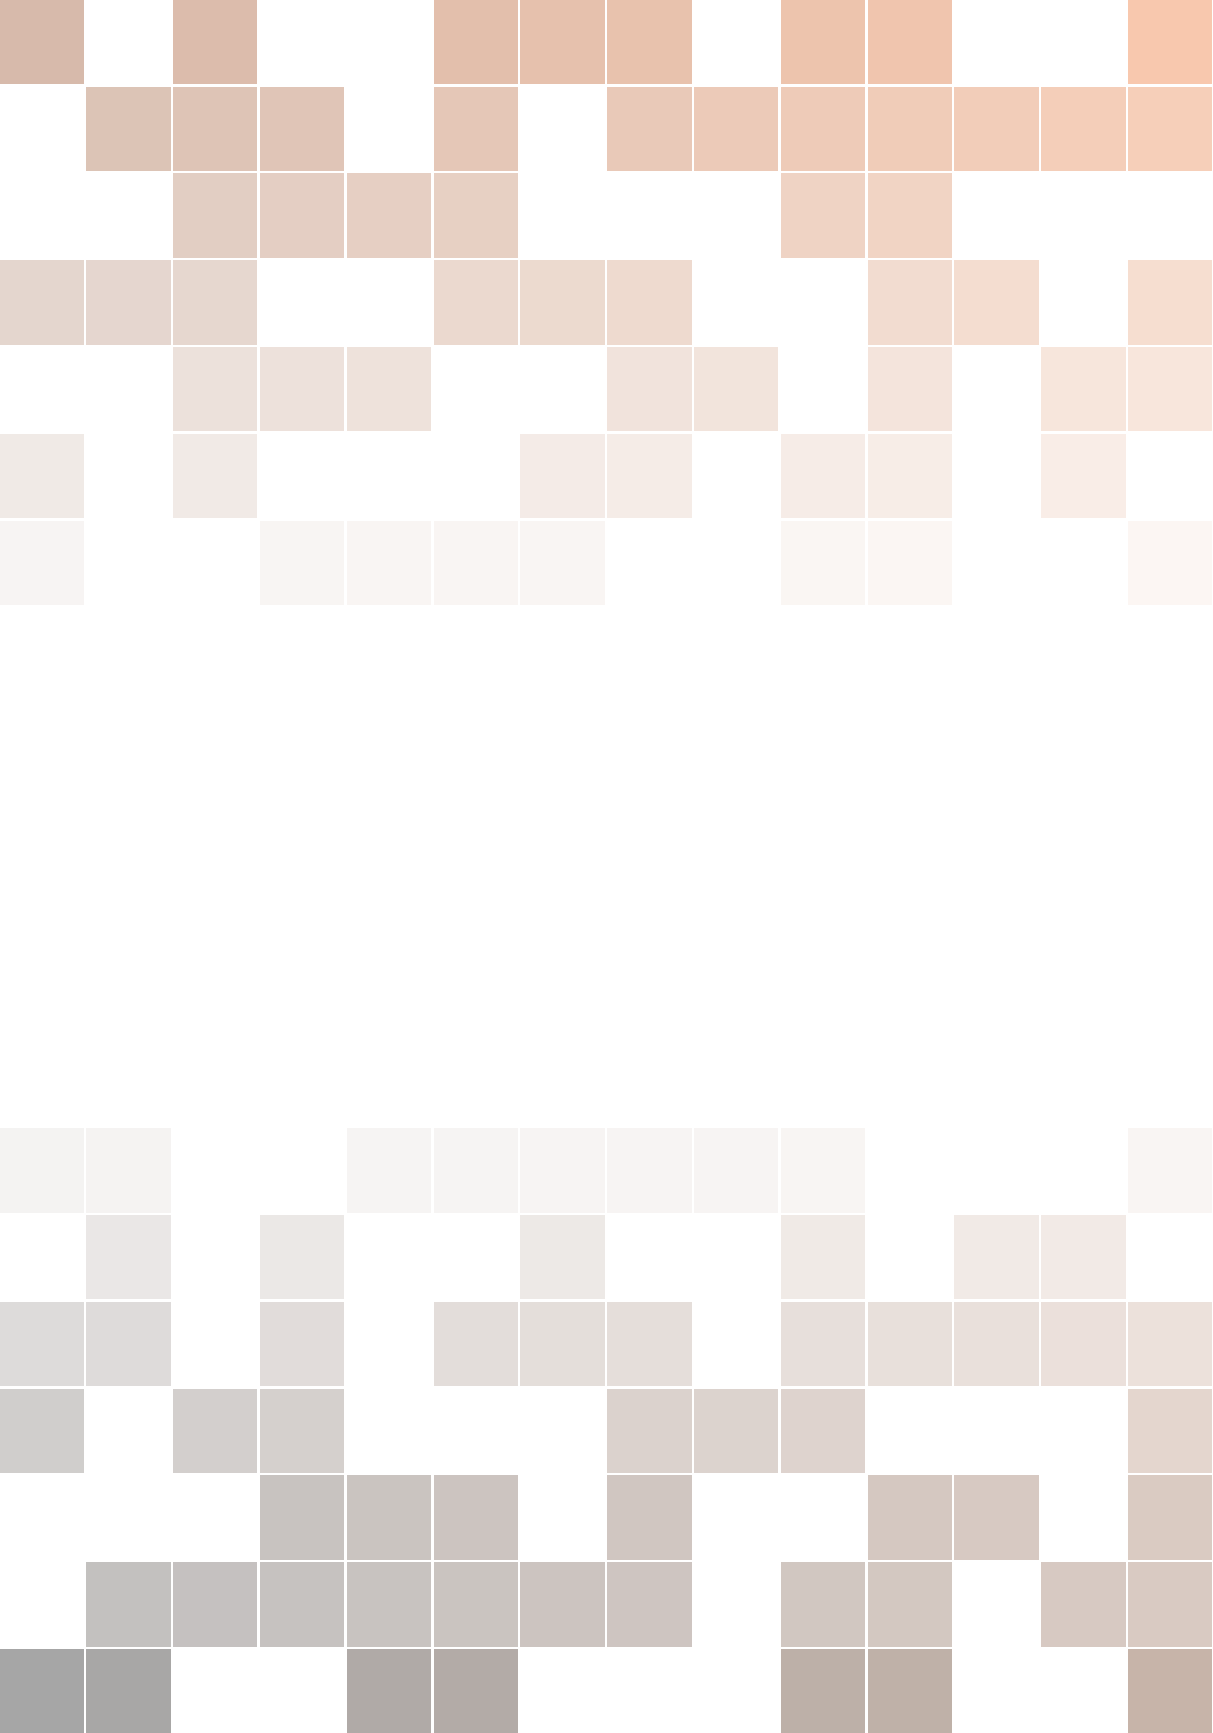
\includegraphics[width=\paperwidth]{poly/Pictures/background.pdf}};
\draw (current page.center) node [fill=ocre!30!white,fill opacity=0.6,text opacity=1,inner sep=1cm]{\Huge\centering\bfseries\sffamily\parbox[c][][t]{\paperwidth}{\centering Signal et Filtrage\\[15pt] % Book title
{\Large IMACS 2ème année}\\[20pt] % Subtitle
{\huge Alexandre Boyer \& Pascal Acco }}}; % Author name
\end{tikzpicture}
\vfill
\endgroup

%-------------------------------------------------------------------------
%	TABLE OF CONTENTS
%-------------------------------------------------------------------------
\usechapterimagefalse % If you don't want to include a chapter image, use this to toggle images off - it can be enabled later with \usechapterimagetrue
%\chapterimage{poly/Pictures/chapter_head_2.pdf} % Table of contents heading image
\pagestyle{empty} % Disable headers and footers for the following pages
\tableofcontents % Print the table of contents itself
\cleardoublepage % Forces the first chapter to start on an odd page so it's on the right side of the book
\pagestyle{fancy} % Enable headers and footers again

%-------------------------------------------------------------------------
%	CHAPITRES
%-------------------------------------------------------------------------
\chapter{Introduction}
	
	Ce cours est une introduction aux concepts et aux outils mathématiques de base de l'analyse des signaux et des systèmes linéaires. Nous préciserons aussi les conditions d'utilisation de ces outils. Même si ils sont centraux dans le traitement du signal, ils sont indispensables dans d'autres disciplines comme l'électronique, l'automatique, la mécanique, les télécommunications ... En effet, les concepts de systèmes et de signaux sont suffisamment généraux pour s'adapter à des domaines différents. La puissance des notions et des outils que nous présenterons dans ce cours est qu'ils peuvent s'appliquer à des domaines, des grandeurs et des objets physiques complètement différents. Ils constituent des outils largement répandus et utilisés non seulement en ingénierie, mais aussi en recherche.	Les concepts vus dans ce cours seront donc utilisés dans les autres enseignements de la 2e année IMACS, mais aussi des prochaines années, et certainement durant toute votre carrière !
	
	Dans ce premier chapitre, nous allons définir les notions de signal, de traitement de signal et de système dit linéaire à temps invariant. Nous terminerons par une présentation des objectifs pédagogiques du cours, de son organisation et des outils utilisés.
	
	

	
	\section{Le signal}
	
	Dans ce cours, on entend par signal tout phénomène physique qui transporte une information. Il indique l'évolution temporel, spatial, d'une ou plusieurs quantités associées à un phénomène physique. Par exemple, il peut s'agir du signal électrique transmis sur un câble réseau ou une onde électromagnétique associée à un réseau WiFi. Les vibrations mécaniques produits par un véhicule, une onde radar, la vitesse de rotation d'un moteur, la température d'une pièce mesurée par un capteur ou un flux de bits lus depuis une mémoire constituent aussi des signaux. Le signal est donc une notion générique provenant de sources physiques très différentes. Pour que ces signaux puissent être traitées et analysées, il faut qu'ils soient mesurés. Pour cette raison, ils sont souvent convertis en signaux électriques.
	
	
	
	
	
	\subsection{Classification des signaux}
	
	Selon sa nature, le phénomène physique, dont le signal constitue la
	signature, peut être exprimé par une fonction mathématique évoluant en
	fonction d'une ou plusieurs variables. Les plus courantes sont des
	variables spatio-temporelles. Dans ce cours, nous traiterons
	principalement de signaux temporels, c'est-à-dire que leur évolution ne
	dépend que du temps, que nous notons s(t). Nous pourrions traiter de la même manière des
	signaux dépendant d'une ou plusieurs variables spatiales, auxquelles on
	pourrait aussi ajouter le temps.
	Considérons que le signal dépend du temps. Nativement, il est exprimé
	dans le domaine temporel, c'est-à-dire que nous pouvons décrire son
	évolution par une fonction dépendante du temps. Nous verrons dans ce
	cours qu'il est possible, via des transformations mathématiques,
	l'exprimer dans un domaine dual, facilitant ainsi son étude ou l'étude
	du système qu'il attaque ou dont il est issu.
	
	Bien que le signal constitue une notion générique qui se ramène à une fonction mathématique, il présente plusieurs caractéristiques que nous allons rapidement présenter.
	
	\subsubsection{Signaux réels ou complexes}
	

	Les signaux physiques sont des signaux réels, c'est-à-dire que les valeurs prises par la fonction $s(t) \in \mathbb{R}$. Cependant, rien n'empêche de définir un signal complexe, dont les valeurs appartiennent à l'ensemble des complexes. L'utilisation des nombres complexes permet la résolution efficace de nombreux problèmes associés à des systèmes physiques. 
	
	\subsubsection{Signaux déterministes ou aléatoires}
	Un signal déterministe présente une évolution parfaitement prédictible. En d'autres termes, on dispose d'un modèle, d'une fonction mathématique permettant de prédire à coup sûr la valeur du signal à un instant donné. A contrario, un signal aléatoire n'est pas prédictible. On peut disposer d'un modèle mathématique décrivant l'évolution du signal, mais on ne peut pas prédire exactement la valeur prise à un instant donné. Il faut noter que la plupart des signaux sont aléatoires : il y a toujours une part d'incertitude dans les phénomènes physiques et les modèles que l'on bâtit pour les étudier sont parfois des approximations. En outre, un signal déterministe n'apporte pas d'informations puisqu'on sait le prédire. 
		
	Le signal déterministe est souvent une abstraction mathématique que l'on rencontre rarement. La figure ci-dessous présente la mesure d'un signal électrique produit par un oscillateur. Ce dispositif produit un signal électrique oscillant à une fréquence fixe. Il est donc parfaitement régulier et facilement modélisable par un signal déterministe. Cependant, la mesure montre une fluctuation aléatoire autour de ce signal, liée au bruit intrinsèque du système de mesure et aux perturbations électriques externes qui se superposent. Ainsi, le signal que l'on mesure devient un signal aléatoire.   
		
	Malgré la nature aléatoire des signaux, nous nous focaliserons uniquement sur des signaux déterministes dans ce cours. Ceux-ci constituent une abstraction mathématique efficace pour étudier les signaux lorsque la nature aléatoire est négligeable. De plus, cela évite l'introduction d'outils statistiques qui compliquerait inutilement ce cours. Les signaux aléatoires seront abordés en 3e année IMACS.


	Figure signal aléatoire

	\subsubsection{Temps continu ou discret}
	Les signaux physiques présentent une évolution continue en fonction du temps ou de l'espace. Avec l'avènement des systèmes de traitement numérique, l'acquisition de ces signaux requiert de ne prélever qu'un nombre fini d'"échantillons" de ce signal. Un échantillon correspond à une valeur prise par le signal à un instant donné. On parle d'échantillonnage. En d'autres termes, le temps est discrétisé. Cet échantillonnage est généralement effectué régulièrement, selon période dite d'échantillonnage.
	On parle alors de signaux à temps discret. En effet, un système de traitement numérique met un temps fini pour effectuer une opération. Pendant ce temps, le signal doit rester fixe, d'où la nécessité de ne traiter qu'un échantillon. De plus, le traitement numérique passe très souvent par la mémorisation. Or, une mémoire numérique présente un nombre fini de "cases mémoires". La différence entre signaux à temps continus et à temps discrets est illustrée à la figure \ref{Fig:Signal_tps_continu_discret}.
	
	\begin{figure}[h!]
		\centering
		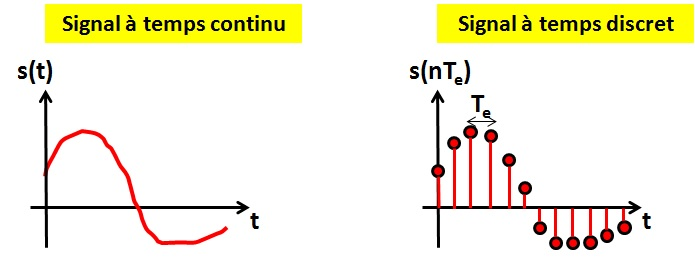
\includegraphics[scale=0.5]{images/Signal_tps_continu_discret.jpg} 
		\caption{Signal à temps continu et à temps discret}	
		\label{Fig:Signal_tps_continu_discret}
	\end{figure}
	
	
	Dans ce cours, nous ne traiterons que des signaux à temps continu. L'effet de l'échantillonnage sur les signaux sera abordé en 3e année IMACS.

	\subsubsection{Signaux à valeurs continues ou discrètes}
	
	La plupart des signaux physiques peuvent prendre une infinité de valeurs à l'intérieur d'un certaine intervalle. On parle alors de signaux à valeurs continues. Cependant, dès qu'un signal doit être traité par un système numérique, celui-ci doit d'abord être encodé sur un nombre fini de bits. Il en résulte un nombre fini d'états que peut prendre le signal. On parle de signal à valeurs discrètes.
	
	En électronique, on distingue ainsi les signaux analogiques, à valeurs et à temps continues, des signaux numériques, à valeurs et à temps discrets.
	
	\subsubsection{Signaux monodimensionnels ou multidimensionnels}
	Un signal peut apporter une information sur l'évolution d'une variable ou de plusieurs variables. Par exemple, le signal peut être l'évolution de la position dans l'espace d'un objet. Le signal contiendra trois variables. De même, un signal peut dépendre d'une ou de plusieurs variables caractérisant son évolution : le temps, l'espace. Dans ce cours et sans perte de généralités, nous ne considérerons que des signaux à une dimension.
	

	
	
	\section{Le traitement du signal}
	
	Le but du traitement de signal est l'analyse et la transformation des signaux en fonctions mathématiques ou paramètres afin d'en extraire l'information. Elle forme une discipline à part entière, et est largement employée dans d'autres domaines, tels que l'électronique, l'automatique, les télécommunications, la thermodynamique, …. Elle est en lien avec les mathématiques mais aussi avec le développement de nouveaux moyens de calcul et de traitements numériques.
	Ses finalités sont nombreuses, on peut citer, entre autres :
	
	\begin{itemize}
		\item l'analyse, c'est-à-dire l'extraction des composantes essentielles portant l'information utile
		\item la mesure, ou l'estimation de grandeurs caractéristiques
		\item la détection et la reconnaissance de signaux, d'informations enfouis
		\item le filtrage, c'est-à-dire l'élimination des composantes "parasites" d'un signal
		\item la restauration d'un signal, liée au processus de filtrage
		\item la synthèse de signaux
		\item le codage, la compression
	\end{itemize}
	
	
	
	Dans ce cours, nous aborderons les outils mathématiques de base d'analyse des signaux. Il s'agit de transformation permettant d'extraire des informations utiles d'un signal. Nous allons notamment aborder l'analyse fréquentielle du signal via la transformée de Fourier. Celle-ci vise à identifier les différentes composantes dites harmoniques qui constituent un signal. L'analyse directe du signal dans le domaine temporel ne permet pas de séparer facilement l'ensemble de ces composantes. L'analyse fréquentielle du signal est souvent l'opération préalable du filtrage, dont le but est l'élimination de signaux indésirables. Bien que son effet soit visible sur l'évolution temporel d'un signal, un filtre est dimensionné à partir de l'analyse fréquentielle de ce signal.
	
	C'est ce qu'illustre la figure \ref{Fig:analyse_spectrale_voix}. L'évolution temporelle montre un signal complexe, difficilement analysable. L'utilisation d'une transformation mathématique, telle que la transformée de Fourier, met en évidence la présence de plusieurs composantes spectrales, à des fréquences harmoniques, qui forment le signal.
	
	\begin{figure}[h!]
		\centering
		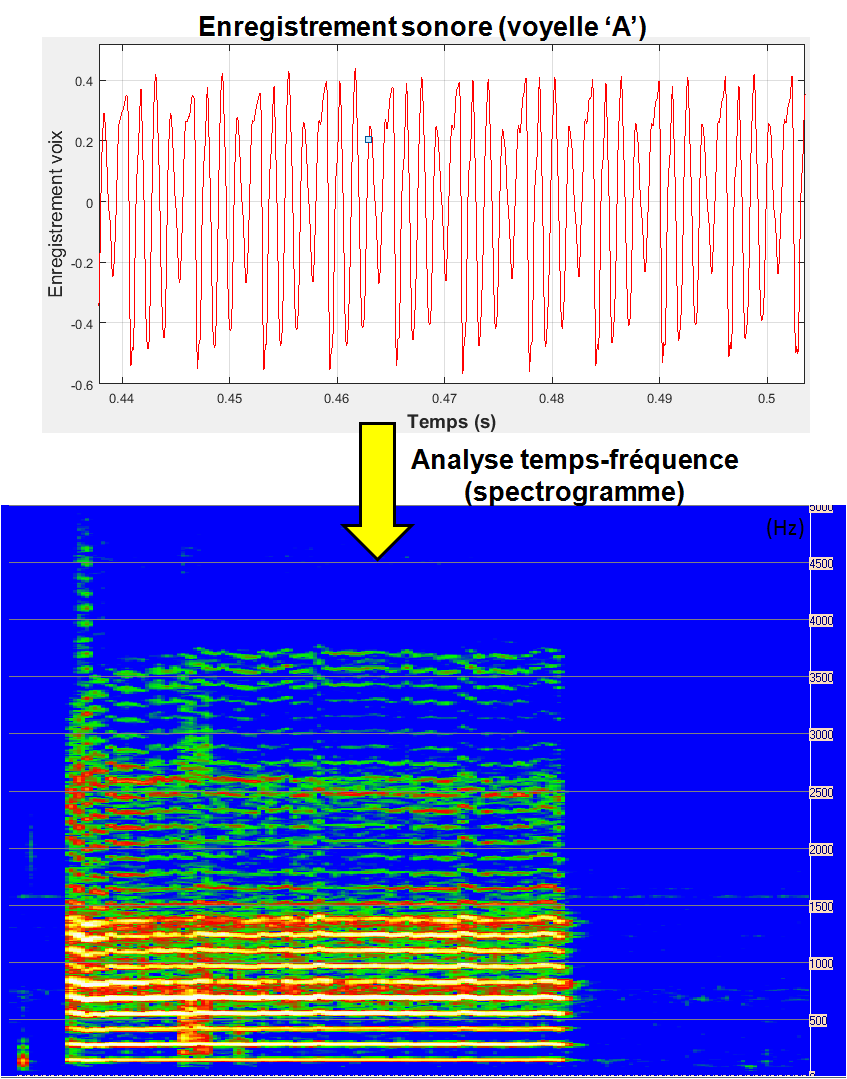
\includegraphics[scale=0.5]{images/spectrogramme_voix.png} 
		\caption{Analyse spectrale de la voix (Logiciel Vocalab, avec la permission d'Etienne Sicard)}	
		\label{Fig:analyse_spectrale_voix}
	\end{figure}
	
	Dans ce cours, la transformée de Fourier ne sera vue que pour des signaux à temps continus. L'impact de l'échantillonnage (ou discrétisation) du signal et sur la transformée de Fourier sera abordé en 3e année IMACS.

	
	\section{Les systèmes linéaires à temps invariant - Réponse d'un système à un signal}
	
	Ce cours a aussi pour but l'étude des systèmes, c'est-à-dire la manière dont ils répondent à un signal d'entrée. Un système est un concept très générique. Ici, nous ne nous intéressons pas à la nature du système et à la compréhension physique de son fonctionnement. Nous pourrons traiter de systèmes électriques, mécaniques, optiques, chimiques, ...	Nous entendons par système le modèle mathématique, abstrait, associé à un objet physique qui décrit son fonctionnement. Il peut être vu comme une "boite" excitée sur son ou ses entrées par un ou plusieurs signaux, comme le montre la figure \ref{Fig:LTI}. L'évolution de sa ou de ses sorties, que l'on appelle réponse, dépend non seulement du signal d'entrée mais aussi des propriétés du système. Ses signaux d'entrée et de sortie peuvent être représentés par des fonctions mathématiques x(t) et y(t). Du point de vue du traitement du signal, un système transforme les signaux. Son effet peut être modélisé par un opérateur mathématique L. Le but de ce cours est de présenter les outils mathématiques permettant de modéliser le système (comment extraire cet opérateur) et de prédire la réponse du système à une excitation donnée. L'objectif est de déterminer un outil mathématique général, fournissant une même méthode de calcul quelle que soit la nature physique du système.
	
	\begin{figure}[h!]
		\centering
		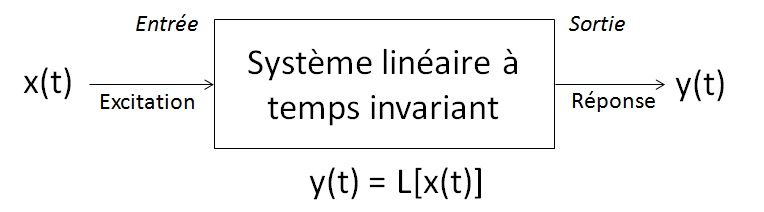
\includegraphics[scale=0.45]{images/LTI.jpg} 
		\caption{Représentation d'un système LTI comme une boîte noire reliant les signaux d'entrée et de sortie par un opérateur linéaire}	
		\label{Fig:LTI}
	\end{figure}


	Dans ce cours, nous traiterons d'une classe de systèmes particuliers, appelés systèmes linéaires à temps invariants (LTI). Les signaux d'entrée x(t) et de sortie y(t) sont reliés entre eux par un ou plusieurs opérateurs linéaires, dont les caractéristiques n'évoluent pas au cours du temps. Si elles sont connues, il devient alors possible de prédire la réponse en sortie du système quelle que soit l'excitation appliquée en entrée. Pour cela, il nous faut déterminer une représentation mathématique de l'effet de ce système, quelle que soit la nature réelle du système. Nous en présenterons deux : l'effet du système LTI sera modélisé par sa réponse impulsionnelle ou sa fonction de transfert. Les outils mathématiques permettant le calcul de sa réponse seront la transformée de Laplace et le produit de convolution.
	
	Comme pour l'analyse fréquentielle, nous ne considérerons que des systèmes à temps continu. Quasiment tous les systèmes ont une évolution continue dans le temps. Cependant, certains d'entre eux se modélisent efficacement en considérant une échelle de temps discrète. C'est notamment le cas pour les circuits électroniques numériques synchrones, dont le fonctionnement logique est cadencé par une horloge périodique. Les concepts présentés dans ce cours devront être adaptés à cette discrétisation du temps. Ces concepts seront abordés en 3e année IMACS. 
	
	

	
	
	
	\section{Les objectifs pédagogiques}
	L'objectif du cours est le suivant : présenter les concepts et les outils de base de l'analyse du signal, ainsi que ceux pour le calcul de la réponse des systèmes linéaires à temps invariant.
	
	A l'issue du cours, vous devrez : 
	\begin{itemize}
		\item (Re)Connaître les différents types de signaux
		\item Calculer le développement en série de Fourier d'un signal périodique et exprimer les coefficients sous ses différentes formes 
		\item Savoir tracer et interpréter une représentation graphique des coefficients de Fourier
		\item Calculer la transformée de Fourier (inverse) d'un signal
		\item Enoncer les principales propriétés de la transformée de Fourier 
		\item Calculer la puissance, l'énergie d'un signal
		\item Enoncer les propriétés d'un système linéaire à temps invariant
		\item Expliquer les notions de réponses naturelles, forcées et d'excitation d'un système naturel, de fréquence naturelle
		\item Connaître les principales familles d'excitation pour l'analyse des systèmes linéaires (exponentiel complexe, impulsionnelle)
		\item Calculer la réponse temporelle d'un système linéaire à partir de la transformée de Laplace (inverse)
		\item Enoncer les principales propriétés de la transformée de Laplace
		\item Déterminer la réponse harmonique d'un système linéaire à partir de sa fonction de transfert
		\item Mettre en œuvre le produit de convolution pour calculer la réponse temporelle d'un système
		\item Déterminer les caractéristiques des filtres linéaires (type, ordre, fréquences de coupure)
		\item Tracer les caractéristiques d'un filtre dans le diagramme de Bode
		\item Calculer la corrélation entre deux signaux
		\item Déterminer la densité spectrale de puissance d'un signal à partir de son autocorrélation
	\end{itemize}
	
	
	\section{Organisation du cours}
	Ce cours s'organise de la manière suivante :
	\begin{itemize}
		\item Nous commençons par l'étude des systèmes linéaires. Le chapitre 2 est dédié à la définition des propriétés des systèmes LTI, des concepts d'excitation et de réponse. Un préalable au calcul de la réponse d'un système est la recherche de type d'excitations qui facilite cette tache. Nous mettrons en évidence deux types de familles d'excitation : exponentielle complexe et impulsionnelle. Elles permettront de définir deux manières complémentaires de modéliser un système : dans le domaine temporel par la réponse impulsionnelle, et dans le domaine fréquentiel par la fonction de transfert.
		\item Le chapitre 3 est consacré à la transformée de Laplace. Cet outil, qui transforme toute fonction mathématique temporelle en une nouvelle fonction exprimée dans le domaine des fréquences complexes, fournit un moyen très efficace pour calculer la réponse transitoire des systèmes LTI, quelle que soit l'excitation appliquée en entrée.
		\item Le filtrage est abordé dans le chapitre 4. Les filtres sont des systèmes LTI comme les autres. La spécificité vient de leur utilisation : l'élimination de composantes fréquentielles indésirables contenues dans un signal. Le dimensionnement d'un filtre passe par une analyse de sa fonction de transfert. Le chapitre présente un outil graphique adapté à l'analyse d'un filtre : le diagramme de Bode, ainsi que le vocabulaire associé à la caractérisation des filtres.
		\item Le chapitre 5 présente la décomposition d'un signal périodique en une série de termes (co)sinusoïdaux, appelée série de Fourier. Celle-ci forme la base de l'analyse fréquentielle du signal. Après une description des différentes formes prises par la série, les principales propriétés des séries de Fourier sont présentées. Plusieurs exemples de décomposition de signaux en série de Fourier sont donnés. Une représentation du signal en spectre de raies est aussi introduite, fournissant un outil d'analyse graphique puissant.
		\item Les séries de Fourier constituent un formidable outil pour l'analyse des signaux, mais ils sont limités aux signaux périodiques. La transformée de Fourier constitue une extension pour tous les signaux. Le chapitre 6 est dédié à la présentation de la transformée de Fourier et son application. Le chapitre montre aussi que la transformée de Fourier est un cas particulier de la transformée de Laplace.
		\item Le chapitre 7 revient sur le calcul de la réponse temporelle des systèmes. Ce point abordé dans le chapitre 3 passait par la transformation du signal dans le domaine fréquentiel, via la transformée de Laplace. Dans ce chapitre, on montre comment ce calcul peut être fait directement dans le domaine temporel. Celui-ci nécessite la mise en œuvre du produit de convolution. 
		\item Dans le dernier chapitre, nous revenons sur les concepts de puissance et d'énergie des signaux. Nous présentons les méthodes de calcul dans les domaines temporels et fréquentiels. Nous introduisons un autre outil fondamental pour l'étude de la ressemblance des signaux : la corrélation. Elle présente aussi un autre intérêt majeur : sa connaissance permet de déterminer la densité spectrale de puissance d'un signal, donnant la répartition de la puissance du signal dans le domaine fréquentiel.
	\end{itemize}
	
	
	\section{Les outils}
	L'analyse des systèmes et le traitement du signal met en œuvre des calculs potentiellement complexes, ne pouvant pas être toujours résolus à la main. Des outils numériques sont donc requis.
	Dans les TD et TP associés à ce cours, nous travaillerons avec Matlab\textsuperscript{\textregistered}, outil de référence pour le calcul numérique et le traitement du signal notamment (fr.mathworks.com). Celui-ci est disponible dans toutes les salles d'informatique de l'INSA. Cependant, il fonctionne avec une licence payante. Un équivalent gratuit, quasiment entièrement compatible, est le logiciel Octave (www.gnu.org/software/octave/). Vous pourrez le télécharger et l'installer sur vos machines personnelles.
		
\cleardoublepage
\usechapterimagetrue
\chapterimage{poly/Pictures/linear_response.png} % Table of contents heading
\chapter{Systèmes linéaires invariants}
\label{chap:lti}
<<<<<<< HEAD
	Le but de ce chapitre est de présenter les concepts de base indispensables à l'étude des systèmes linéaires à temps invariants (LTI) et des signaux.
	Après une définition des critères qui caractérisent un système LTI, nous chercherons à répondre à la question suivante :
	comment déterminer efficacement la réponse d'un système linéaire lorsqu'il est soumis à une excitation quelconque ? Par efficacement, nous entendons :
	\begin{itemize}
		\item méthode mathématiquement "simple"~;
		\item méthode indépendante de l'excitation et des propriétés du système LTI.
	\end{itemize}

%	\vspace{1\baselineskip}
	
	Pour cela, nous commencerons par nous interroger sur la manière de représenter l'interaction entre l'entrée et la sortie d'un système, puis sur les notions d'excitation et de réponse. Nous distinguerons les notions de réponses naturelles et forcées, avant d'identifier deux familles d'excitation adaptées à l'étude des systèmes : exponentielle complexe et impulsionnelle. Nous introduirons ensuite la notion de fréquence (complexe), qui nous offrira la possibilité d'étudier les signaux temporels dans le domaine fréquentiel, ainsi que la notion de fonction de transfert qui facilitera l'étude des systèmes.
	
	
	\section{Définition d'un système linéaire à temps invariant}
=======
Le but de ce chapitre est de présenter les concepts de base
indispensables à l'étude des systèmes linéaires à temps invariants
LTI\footnote{ Linear Time Invariant} et des signaux.  Après une
définition des critères qui caractérisent un système LTI, nous
chercherons à répondre à la question suivante : comment déterminer
efficacement la réponse d'un système linéaire lorsqu'il est soumis à
une excitation quelconque ?  Par efficacement, nous entendons :
\begin{itemize}
\item méthode mathématiquement "simple"~;
\item méthode indépendante de l'excitation et des propriétés du
  système LTI.
\end{itemize}


Pour cela, nous commencerons par nous interroger sur la manière de
représenter l'interaction entre l'entrée et la sortie d'un système,
puis sur les notions d'excitation et de réponse. Nous distinguerons
les notions de réponses naturelles et forcées, avant d'identifier deux
familles d'excitation adaptées à l'étude des systèmes : exponentielle
complexe et impulsionnelle. Nous introduirons ensuite la notion de
fréquence (complexe), qui nous offrira la possibilité d'étudier les
signaux temporels dans le domaine fréquentiel, ainsi que la notion de
fonction de transfert qui facilitera l'étude des systèmes.
	
	
\section{Définition d'un système linéaire invariant}
>>>>>>> 32c0df24da5390795360e6583dca2c28be03f1cf

	\subsection{Linéarité} 
	Un système relie à chaque signal d'entrée $x$ un signal de
        sortie unique $y$. Les signaux $x$ et $y$ sont des fonctions
        de la variables réelle appartenant à un espace de fonction le
        plus général possible noté ici $L_E$. La relation
        entrée-sortie est donc modélisée par une application
        mathématique de $L_E$ dans $L_E$ notée $L$ et définie ainsi~:
	\begin{equation}
          L : \application{L_E}{L_E}{x : t\mapsto x(t)}{y : t\mapsto y(t)} 
          % DONE : correction TYPAGE et remarque notation
	\end{equation}
<<<<<<< HEAD
	\begin{remark}{}
	    Remarquons que l'application $L$ transforme une fonction en une fonction et que cela peut compliquer les notations, aussi il est courant de voir utiliser les crochets [] autour des fonctions arguments de l'application $L$ et les simples parenthèses autour de la variable réelle argument d'une fonction. Ce genre d'application est souvent désignée par le terme d'\emph{opérateur}
=======

	\begin{remarque}{}
          Remarquons que l'application $L$ transforme une fonction en
          une fonction et que cela peut compliquer les notations,
          aussi il est courant de voir utiliser les crochets [] autour
          des fonctions arguments de l'application $L$ et les simples
          parenthèses autour de la variable réelle argument d'une
          fonction. Ce genre d'application est souvent désignée par le
          terme d'\emph{opérateur}
>>>>>>> 32c0df24da5390795360e6583dca2c28be03f1cf
	    
          Beaucoup d'abus de notation figurent dans la littérature,
          gardons à l'esprit et tentons cette année encore de
          conserver une rigueur d'écriture irréprochable pour garder
          les idées claires. Parmi les écritures suivantes, une est
          parfaitement correcte et représente un réel~; une représente
          correctement une fontion mais ne respecte pas la convention
          des crochets~; une est incorrecte~; une est correcte mais
          lourde à écrire. À vous de les retrouver~:
          \begin{itemize}
          \item $y(t) = L[x(t)]$~;
          \item $y = L(x)$~;
          \item $y(t) = L[x](t)$~;
          \item $t\mapsto y(t) = L[t\mapsto x(t)]$
          \end{itemize}{}
	\end{remarque}
	
	Une classe de système fondamentale est la classe des systèmes
        linéaires car elle offre de nombreux outils et propriétés
        mathématiques.
	\begin{definition}{Système linéaire}
          \label{def:linearite}
          
          Une système est dit linéaire si et seulement si
          l'application $L$ associée est linéaire, soit pour tout
          $\p{x_1,x_2,\lambda} \in L_E^2 \times \R$~:
          \begin{eqnarray}
            \label{eq:def_linearite}
	    \forall t \in \R \qquad L\b{x_1 + \lambda\, x_2}(t) = L\b{x_1}(t) + \lambda\,L\b{y_2}(t) \nonumber\\
	    \text{ou bien } \qquad L\b{x_1 + \lambda\,x_2} = L\b{x_1} +\lambda L\b{x_2 }
          \end{eqnarray}
	\end{definition}
	

	Une des conséquences de la linéarité est la possibilité
        d'appliquer le principe de superposition.
	
	% TODO on va considérer d'autres systèmes ! j'enlèverai cette
	% partie qui n'amène pas grand chose...
	Les trois opérateurs linéaires de base que nous considérons
        dans l'étude des systèmes linéaires sont :
	\begin{itemize}
        \item proportionnel : $y = a x$ où a est une constante
        \item intégration : $y = a \int f(x) \deriv x $ où a est
          une constante
        \item dérivée : $y = a \frac{df(x)}{dx} $ où a est une
          constante
	\end{itemize}
	On peut aisément vérifier qu'il respecte la condition
        \ref{eq:def_linearite}.
	% Fin du dodo

        \begin{remarque}
          Pour résoudre les complexes équations différentielles des
          télégraphistes, \Heaviside{} utilise ces opérateurs de base
          et introduit le \emph{calcul symbolique}. Cela consiste à
          représenter l'application de l'opérateur dérivée sur une
          fonction $f$ comme une simple multiplication par un nombre
          $p$. Ainsi une équation différentielle
          $a\,y'' + 2y' -y = 3\int x$ est associée à l'équation
          symbolique $a\,p^2\,y + 2\,p\,y - y = \frac{3}{p}x$. Il est
          alors possible de résoudre algébriquement l'équation sous
          forme de fractions rationnelles ce qui donnerait avec notre
          exemple~: $y = \frac{3/p}{a\,p^2+2p+1} x$. Rappelons que $x$
          et $y$ sont des fonctions et non des réels et que dans ce
          cas les opérations ne sont pas de simple multiplication et
          addition de réels mais bien des multiplications et additions
          de fonctions. La variable symbolique $p$ est utilisée comme
          un nombre réel mais n'est en aucun cas un réel...
        \end{remarque}
	
	\subsection{Invariance temporelle}
	% DONE rédaction en définition
	Il est fréquent qu'un système réagisse de la même manière
        indépendemment de l'instant où est appliqué le signal
        d'entrée. Ce qui conduit à la définition suivante~:
	\begin{definition}{Système invariant dans le temps}
          
          Un système est dit invariant dans le temps si et seulement
          si son application associée $L$ vérifie~:
          \begin{equation}
            \forall x\in L_E, \forall (t,t_0)\in \R^2, \quads L[t\mapsto x(t-t_{0})] = L[x](t-t_{0}) 
          \end{equation}
	\end{definition}
	
	En d'autres termes, la réponse du système ne dépend pas de
        l'origine des temps choisie.
        
	\begin{exemple}
          % TODODONE typage !!!
          L'effet d'un système sur le signal d'entrée est d'écrit par
          l'application ~: $x \mapsto y=2\dDtDe{x}$.  Vérifions
          d'abord que cet opérateur est linéaire~:
          \begin{eqnarray*}
            L\b{x_1+\lambda x_2} &= t \mapsto 2\, \dDt\p{x_1+\lambda x_2}\\
                                 &= t \mapsto 2\,\dDtDe{x_{1}} + 2\lambda\,\dDtDe{x_{2}}\\
                                 &= L\b{x_{1}}+\lambda\,L\p{x_{2}}
          \end{eqnarray*}
          Le système est donc linéaire. Vérifions qu'il est
          invariant~:
          \begin{equation*}
            \forall t \quads L\b{t\mapsto x(t-t_{0})}(t) =2\,\dDe{x\p{t-t_0}}{\p{t-t_0}}\,.\,\underbrace{\dDe{\p{t-t_0}}{t}}_{=1}=2\dDtDe{x}\p{t-t_0}=L\b{x}\p{t-t_0}
          \end{equation*}
          ou bien exprimé par le biais des opérateurs en exprimant le
          retard d'un temps $t_0$ par le biais de l'application
          identité soit $\Id-t_0 : t \mapsto t - t_0$ ~:
          \begin{equation*}
            L\b{t\mapsto x(t-t_{0})} = L\b{x \circ \p{\Id-t_0}}=2\,\dDt\p{x\circ\p{\Id -t_{0}}}=2\,\dDtDe{x}\circ\p{\Id-t_0}\,.\,\underbrace{\dDt\de{\Id-t_0}}_{=1}=L\b{x}\circ\p{\Id-t_0}
          \end{equation*}
        \end{exemple}
	
        % TODODONE pas d'accord là ! Un simple gain de 2 est un
        % système qui n'est pas passif...
        % à discuter
        %	\subsection{Passivité}
        %	Dans ce cours, on considèrera aussi des systèmes
        % passifs, dans le sens où il n'y a pas d'énergie emmagasinée
        % ou fournie par une entrée autre que celle sur laquelle on
        % applique le signal d'entrée étudié.
      
	\subsection{Causalité}
	L'étude des systèmes linéaires passent par l'étude et la
        synthèse de fonctions mathématiques. Tous les systèmes
        linéaires physiquement réalisables peuvent être décrits par
        une fonction mathématique linéaire. Par contre, la réciproque
        n'est pas forcément vraie : un système décrit par une fonction
        linéaire n'est pas nécessairement physiquement réalisable. Une
        caractéristique importante qui différencie les systèmes
        physiquement réalisables de ceux qui ne le sont pas est la
        notion de causalité. On entend par physiquement réalisable un
        système pouvant traiter en temps réel les signaux d'entrée.
        Dans un système causal, l'effet ne peut pas précéder la cause,
        ce qui donne la définition suivante.
        \begin{definition}{Système causal}
          \label{def:causal}
          
          Un système est causal si, et seulement si, la propriété suivante est vérifiée pour tout $t_0 \in\R$~:
          \begin{equation}
            \label{eq:def_causal}
          \forall t<t_{0} ,\;  x(t) = 0 \quads\implies\quads \forall t<t_{0},\; y(t) = 0
	\end{equation}   
        \end{definition}

       	Les systèmes numériques peuvent être non causaux car ils sont
        capables de stocker les valeurs du signal d'entrée pour un
        traitement différé. On peut prendre l'exemple de l'application
        de floutage d'une image numérique. Celle-ci correspond à une
        matrice de données, représentant chaque pixel de l'image. Le
        floutage consiste à appliquer un filtre (par exemple gaussien)
        qui sera centré sur chaque pixel. Ce filtre effectue une somme
        pondérée du pixel central mais aussi des pixels voisins,
        situés avant et après le pixel central. L'effet du floutage
        d'un pixel dépend donc de pixels situés après dans l'ordre de
        rangement des pixels.

	
	
	\section{Equation générale d'un système linéaire}
        Un système linéaire invariant est gouverné par une équation
        différentielle à coefficient constant donnée dans sa forme
        générale par \ref{eq:generale_lti}. On l'appelle l'équation
        générale du système. Pour une excitation $x(t)$ donnée, sa
        résolution permettra de déterminer la réponse $y(t)$.	
	\begin{eqnarray}\label{eq:generale_lti}
          L : x \mapsto y \text{ telle que }\quads &\sum_{n=0}^N{a_{n}\,\dDtDeOrdre{y}{n}} = \sum_{m=0}^M b_{m}\, \dDtDeOrdre{x}{m}\\\nonumber
       \iff & a_0\,y + a_1\,\dDtDe{y} +\ldots + a_{N}\,\dDtDeOrdre{y}{N} = b_0\,x + b_1\,\dDtDe{x} +\ldots + b_{M}\,\dDtDeOrdre{x}{M} 
        \end{eqnarray}
	
	
	\section{Réponse d'un système}
	La réponse d'un système correspond au signal (ou aux signaux)
        de sortie lorsqu'il est excité par un (ou plusieurs) signal
        d'entrée. En reprenant l'équation générale
        \ref{eq:generale_lti}, on remarque que l'on peut
        distinguer :
	\begin{itemize}
        \item une réponse propre ou naturelle d'un système, notée
          $y_{H}(t)$, correspondant à une solution de l'équation
          différentielle homogène~: \cad{} pour une excitation nulle.
        \item la réponse forcée, notée $y_{f}(t)$ correspondant à la
          solution particulière de l'équation différentielle associée
          à une excitation particulière $x(t)$.
	\end{itemize}
	
	La réponse naturelle $y_h$ appartient à un espace des
        solutions homogènes noté $S_H$ et sera déterminée en fonction
        des conditions initiales. La réponse d'un système sera la
        superposition de ces deux réponses.
	\begin{equation}
          y(t) = \underbrace{y_{H}(t)}_{\in S_H} + y_{f}(t)          
	\end{equation}
	
	Dans la suite du cours, nous ne nous intéresserons qu'à des
        systèmes causaux, et nous considérerons, sans perte de
        généralité, que les excitations sont nulles pour $t < 0$.
	
	\section{Réponse naturelle d'un système LTI}
	Il s'agit de la partie de la réponse qui est indépendante de
        l'excitation, \cad{} la solution de l'équation homogène. Elle
        est donc intrinsèque aux caractéristiques du système. Elle se
        détermine en résolvant l'équation différentielle
        \ref{eq:generale_lti} dans le cas où l'excitation $x(t)$ est
        nulle.
	\begin{equation}\label{eq:reponse_naturelle}
          \sum_{n=0}^N a_{n}\, \dDtDeOrdre{y}{n} = 0
	\end{equation}

        % %%TODO petite erreur, je parlerai des conditions initiales ici
	% On pourrait s'interroger sur le sens de cette réponse. Si le
        % système n'avait pas emmagasiné d'énergie au départ, la réponse
        % serait nulle, ce qui ne présente pas d'intérêt pour l'étude
        % des systèmes. La réponse naturelle n'apparait que si le
        % système a été préalablement excité avant t = 0.
        % DONE je propose
        \begin{remarque}
          On peut s'interroger sur le sens physique de la recherche
          d'une solution non--nulle pour $t>0$ alors que le système
          n'est pas excité (un second membre nul correspondant à une
          entrée nulle). L'intuition physique nous laisse penser
          qu'une réponse non nulle n'apparaîtrait que si le système a
          été préalablement excité avant ou pendant $t = 0$, puis \og
          relâché \fg{} par une excitation nulle pour tout $t>0$.

          Lorsque l'on ne souhaite pas s'intéresser à ce qui précède
          l'instant $t_0=0$ et à ce qui a pu amener le système dans un
          état d'excitation (énergie emmagasinée dans les composants
          etc.), on considère alors une excitation et une réponse
          nulle pour tout $t<t_0$ et on ajoute des conditions
          initiales non nulles à l'instant $t_0$ représentant l'état
          du système (tensions et courant initiaux dans un système
          électrique par exemple) avant le lâché à l'instant $t_0$.
      \end{remarque}

        
        % %%TODO ben non ! elle apparait à t>0... peut être parler
        % %% des manières d'ammener un système à son état initial...
	% Comme l'excitation disparait pour t > 0, la réponse sera
        % forcément transitoire. Seule une fonction présentant la même
        % forme avant/après dérivation plusieurs fois peut être solution
        % de l'équation \ref{eq:reponse_naturelle}. Il n'existe
        % qu'une seule forme de fonction avec une telle propriété : la
        % forme exponentielle complexe donnée par (\ref{expo_complexe}).

        %% TODO le faire en annexe 
        %%TODO et si on disait qu'on s'intéresse aux solutions de formes
        %% exponentielle : on le justifie par l'expérience et en math par
        %% par un passage de l'équadiff à une forme matricielle compagne.
        % DONE je propose

      Rappelons que pour les équations différentielles d'ordre 1,
      l'espace des solutions homogènes est généré par toute
      combinaison linéaire d'une seule solution
      $y_0$ de forme exponentielle réelle~:
      \begin{equation}
        \label{eq:sol_homogene_ordre_1}
        S_H=\a{\lambda y_0|\lambda\in\R}=\vect{y_0},\quads \text{avec } L\b{y_0}=\nullDe{L_E},\quads \text{et } y_0: t\mapsto \expo{\alpha\,t},\;\alpha \in \R 
      \end{equation}

      Dans le cas d'équations d'ordre supérieur, la recherche de
      solutions de forme exponentielle non nulles
      $t\mapsto \expo{p\,t}$ vérifiant l'équation homogène donne en
      remplaçant dans \eqref{eq:reponse_naturelle}~:
      \begin{eqnarray} \label{solution_reponse_naturelle} \forall
        t\in\R,\quads \sum\limits_{n=0}^N a_{n}\,\dDtDeOrdre{\expo{p
            t}}{n} =
        \sum\limits_{n=0}^N a_{n}\,p^{n} \expo{p\,t} =\underbrace{\expo{p\,t}}_{\neq 0}\;\sum\limits_{n=0}^N a_{n}\,p^{n}  =0\\
        \implies D(p)= \sum_{n=0}^N a_{n} p^{n} = 0
      \end{eqnarray}

      Le polynôme $D(p)$ est appelée l'équation caractéristique du
      système d'équations différentielles. Pour un système d'ordre
      $N$, ce polynôme est scindé dans $\C$ et possède donc $N$
      racines réelles ou complexes conjuguées telle que
      $D(p)=a_N\,\prod\limits_{i=1}^{N-1}\p{p-p_i}$. Ces racines sont appelées
      pôles du système et notées $p_i$ (i de $1$ à $N$). Les
      caractéristiques de la réponse naturelle du système sont liées
      uniquement aux $N$ solutions, ou pôles $p_{i}$, de cette
      équation.

      % La réponse naturelle peut alors s'écrire sous la forme suivante~:
	% \begin{equation}\label{reponse_naturelle}
        %   y_{H}(t) = \sum_{i=1}^N A_{i} \expo{p_i\,t}
	% \end{equation}
	% où les termes $A_{i}$ dépendent des conditions initiales
        % connues en un temps $t_{0}$.	
	% Ce polynôme est appelée l'équation caractéristique du
        % système. En effet, les caractéristiques de la réponse
        % naturelle du système sont liées aux M solutions ou racines
        % $p_{i}$ de cette équation. La réponse naturelle peut alors
        % s'écrire sous la forme suivante :
	% \begin{equation}\label{reponse_naturelle}
        %   y_{0}(t) = \sum_{i=1}^M A_{i} \expo{p_i\,t}
	% \end{equation}
	% où les termes $A_{i}$ dépendent des conditions initiales
        % connues en un temps $t_{0}$.	
        
      On montre que les solutions homogènes des équations
      différentielles d'ordre $N$ à coefficients constants sont des
      combinaisons linéaires de $N$ exponentielles $y_i$ à
      coefficients réels et/ou paire de complexes conjuguées. L'espace
      des solutions homogènes est donc un espace de dimension $N$
      généré par la famille $\a{y_i}_{i=1\dots N}$ de $N$
      exponentielles complexes~:
	\begin{equation}\label{eq:sol_homogene_ordre_n}
          S_H=\vect{\a{y_i}_{i=1\dots N}},\quads \text{avec } L\b{y_i}=\nullDe{L_E}\quads\text{et }y_i : t\mapsto \expo{p_i\,t},\quads p_i\in\C     
	\end{equation}

        La réponse naturelle peut alors s'écrire sous la forme
        suivante~:
	\begin{equation}\label{eq:reponse_naturelle}
          \forall t\in\R,\quads y_{H}(t) = \sum_{i=1}^N \lambda_{i} \expo{p_i\,t}
	\end{equation}
	où les termes $\lambda_{i}$ dépendent des conditions initiales
        connues en un temps $t_{0}$.	
        
	\subsection{Fréquences naturelles d'un système LTI}
	Les $N$ racines de l'équation caractéristique du systèmes sont
        appelées les fréquences naturelles ou fréquences propres du
        système. Elles sont complexes et de la forme suivante :
	\begin{equation}\label{freq_propre}
          p_{i} = \sigma_{i} + j\omega_{i} 
	\end{equation}	
	En reprenant \ref{eq:reponse_naturelle}, la réponse naturelle
        pourra s'exprimer en fonction de ces fréquences naturelles :		
	\begin{equation}\label{eq:reponse_naturelle_freq}
          y_{0}(t) = \sum_{i=1}^M \lambda_{i}\expo{\sigma_{i}t}\,\expo{j\omega_{i}t}
	\end{equation}
	$\omega_{i}$ caractérise la pulsation de la réponse associée à
        cette racine, tandis que la partie réelle $\sigma_{i}$ indique
        l'atténuation ou l'amortissement de cette réponse. Leur
        connaissance est indispensable car ce sont elles qui
        caractérisent la forme temporelle de la réponse du système. La
        prédiction de l'évolution temporelle de la réponse du système
        va passer par l'analyse de ces racines.
	
	\subsection{Plan de \Laplace}
	Puisque les racines de l'équation caractéristique déterminent
        la réponse naturelle d'un système, il est intéressant
        d'établir un système de représentation graphique facilitant
        l'analyse du système. C'est le but de la représentation
        appelée plan complexe, plan de \Laplace{} ou plan P, illustré
        à la figure \ref{Fig:Plan_P}. Il s'agit d'un repère cartésien
        dans lequel les racines sont placées, permettant de visualiser
        leurs parties réelles et imaginaires. Selon le positionnement
        des racines dans le plan complexe, les caractéristiques du système
        seront différentes, notamment sa stabilité.
	\begin{figure}[htbp]
          \centering 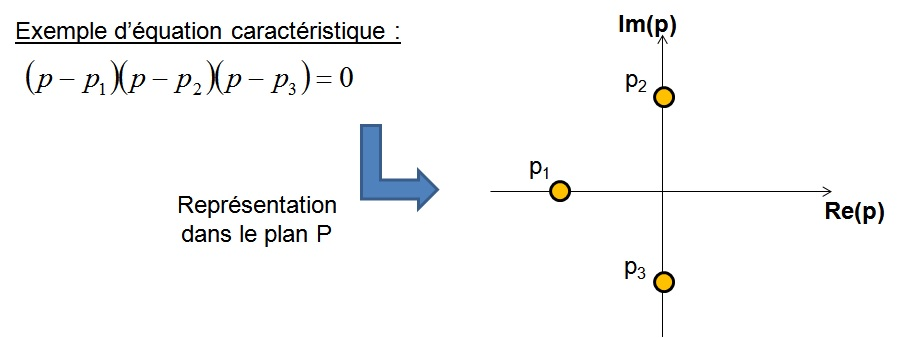
\includegraphics[scale=0.5]{images/Plan_P.jpg}
          \caption{Placement des racines de l'équation caractéristique
            dans le plan complexe. La racine $p_1$ est réelle
            négative~: apportant une exponentielle décroissante à la
            réponse. Tandis que $p_2$ et $p_3$ sont purement complexes
            conjuguées et apportent deux exponentielles complexes
            conjuguées, et donc par la formule d'\Euler{} une forme
            sinusoïdale pure, à la réponse.}
          \label{Fig:Plan_P}
	\end{figure}

	% \subsection{Analyse du plan complexe - Stabilité du système}
        % %%TODO def de strabilite fausse
	% La stabilité d'un système est une notion qui sera abordée plus
        % en détail dans les cours d'automatique. Dans ce cours, nous
        % utiliserons une définition au sens large : on entend par
        % stabilité le fait que la réponse d'un système converge vers
        % une valeur finie quelle que soit l'excitation appliquée (à
        % condition que cette excitation converge). Dès que l'on conçoit
        % un système, c'est une propriété indispensable qui doit être
        % vérifiée.  Un système est stable si et seulement si à toute
        % entrée bornée, il fait correspondre une sortie bornée :
        % DONE je preprend en proposant

        La stabilité d'un système est une notion qui sera abordée plus
        en détail dans les cours d'automatique, il s'agit en fait
        d'une propriété intrinsèque du système ne dépendant pas de
        l'excitation. Dans ce cours, nous utiliserons une définition
        au sens large~: on entend par stabilité le fait que la réponse
        naturelle ne diverge pas. Dès que l'on conçoit un système,
        c'est une propriété indispensable qui doit être vérifiée.

        \begin{definition}{stabilité d'un système}
          \label{def:stabilite}
          
          Un système est stable si, et seulement si, à toute entrée
          bornée, il fait correspondre une sortie bornée~:
	\begin{equation}
          \exists A\in\R,\;\forall t \in \mathbb{R},\quads \abs{x(t)} \leq A \quads\implies\quads \exists B\in\R,\; \forall t\in\R,\quads \abs{y(t)} \leq B
	\end{equation}
        \end{definition}

        Dans le cas des systèmes LTI, cette définition est équivalent
        à la définition suivante~: un système est stable si toute
        réponse naturelle tends vers 0 à l'infini. Dans ce cas là la
        notion de stabilité est clairement indépendante du type
        d'excitation.

        La position des racines de l'équation caractéristique
        détermine à la fois la stabilité du système linéaire, mais
        aussi la forme temporelle de réponse.

        La figure ci-dessous illustre les types de réponse naturelles
        associées à une fréquence naturelle, selon sa position dans le
        plan complexe.
	\begin{figure}[htbp]
          \centering
          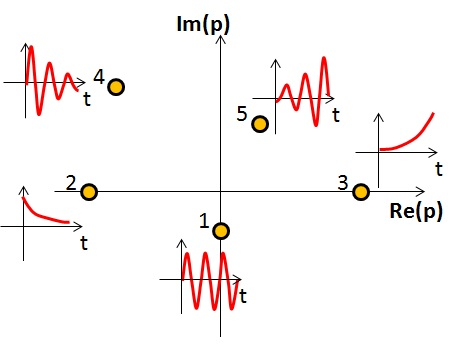
\includegraphics[scale=0.5]{images/reponse_vs_p.jpg}
          \caption{Types de réponse naturelle en fonction de la
            position d'une racine dans le plan complexe.}
          \label{Fig:reponse_vs_p}
	\end{figure}
        Considérons les cinq cas suivants, correspondant à cinq
        positions différentes d'une racine $p_{i}$ dans le plan
        complexe, et déterminons le type de réponse temporelle. On
        considère t > 0 :
	\begin{enumerate}
        \item $p_{i}$ est purement complexe ($\sigma_{i}$ = 0) : elle
          est située sur l'axe des ordonnées du plan complexe. La réponse
          naturelle sera donc un signal purement (co)sinusoïdale, dont
          l'oscillation aura une fréquence ou une pulsation déterminée
          par $\omega_{i}$. Le système est en limite de stabilité car
          sa réponse oscille en permanence autour d'une valeur.
        \item $p_{i}$ est purement réel et négatif ($ \sigma_i\leq 0$
          et $ \omega_i = 0$)~: la racine est située sur l'axe des
          abscisses à gauche de l'origine. La réponse est une fonction
          exponentielle décroissante, sans la moindre oscillation,
          indiquant un comportement amorti. Le système est stable
          asymptotique.
        \item $p_{i}$ est purement réel et positif ($ \sigma_i\geq 0$
          et $ \omega_i = 0$)~: la racine est située sur l'axe des
          abscisses à droite de l'origine. La réponse est une fonction
          exponentielle croissante, sans la moindre oscillation,
          indiquant un comportement divergeant. La réponse naturelle
          indique un système instable.
        \item $p_{i}$ est une valeur complexe quelconque dont la
          partie réelle est négative ($ \sigma_i< 0$ et
          $\sigma_{i} \neq 0 $) : la racine est située dans le demi
          plan à gauche de l'axe des ordonnées. La réponse va
          présenter une oscillation dont la fréquence est déterminée
          par $ \omega_{i}$, mais dont l'amplitude s'atténue
          exponentiellement plus ou moins rapidement au cours du temps
          selon la valeur $\sigma_{i}$. Cette réponse indique un
          système stable oscillatoire amortis.
        \item $p_{i}$ est une valeur complexe quelconque dont la
          partie réelle est positive ($\sigma_i > 0$ et
          $ \omega_{i} \neq 0 $) : la racine est située dans le demi
          plan à droite de l'axe des ordonnées. La réponse va présenter
          une oscillation dont la fréquence est déterminée par
          $ \omega_{i} $, mais dans l'amplitude s'accroît exponentiellement plus ou
          moins rapidement au cours du temps selon la valeur
          $\sigma_{i}$. Cette réponse indique un système oscillatoire instable.
	\end{enumerate}

        % %TODO comprend pas trop l'objectif final... me parait dangereux...
	% \textbf{\underline{Domaine fréquentiel}}	
	% On remarque que l'on est capable de représenter avec un point
        % dans le plan p une fonction temporelle de type exponentielle
        % complexe. Il s'agit de la même fonction, mais vue dans un
        % autre domaine, que l'on appelle domaine fréquentiel. Dans ce
        % domaine, la fonction n'est plus caractérisée par le temps,
        % mais par sa fréquence. De manière générale, les fréquences
        % sont des grandeurs complexes. Néanmoins, dans le cas de
        % l'analyse des signaux, on ne considère que des fréquences
        % réelles.
	
	
	\subsection{Ordre d'un système linéaire}
	Plus l'équation caractéristique présente de racines, plus sa
        réponse devient complexe, puisqu'elle résulte de la
        superposition de plusieurs fréquences comme le montre
        l'équation \ref{eq:reponse_naturelle}. On appelle l'ordre d'un
        système le nombre de racines que présente son équation
        caractéristique. Il s'agit aussi de l'ordre ou du degré de
        l'équation différentielle caractérisant le système. Pour
        illustrer la notion d'ordre, nous allons analyser la réponse
        naturelle de deux circuits électriques passifs, caractérisés
        par des équations caractéristiques d'ordre 1 et 2. Vous
        retrouverez une analyse plus détaillée dans le cours
        d'électronique.
	
        \begin{exemple}{circuit RC}
          \label{ex:circuit_rc}
          
          \begin{minipage}[l]{0.7\linewidth}
            On considère le circuit ci-contre, formé par une résistance
            R et un condensateur C. En t = 0, le condensateur est
            chargé, de sorte que la tension à ses bornes soit égale à
            $U_{C0}$. On note $U_{C}$ et $U_{R}$ les tensions aux bornes
            du condensateur et de la résistance.
          \end{minipage} \hfill
          \begin{minipage}[r]{0.4\linewidth}
            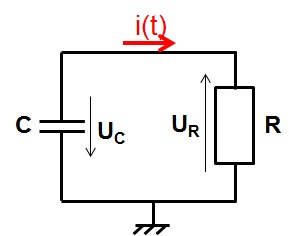
\includegraphics[scale=0.5]{images/circuit_RC_reponse_naturelle.jpg}
          \end{minipage}
          
          On souhaite déterminer la réponse naturelle de ce circuit pour
          $t > 0$, sous la forme du courant électrique $i(t)$ circulant au
          travers du circuit. On souhaite aussi déterminer la fréquence
          naturelle de ce circuit, caractérisant sa réponse transitoire.
          
          
          Commençons par appliquer la loi des mailles à ce circuit, qui
          permet d'écrire : $U_{R}(t)+U_{C}(t)=0.$ En prenant en compte
          les relations tension-courant pour la résistance et le
          condensateur, cette relation peut être mise sous la forme
          ci-dessous ne faisant apparaître que le courant. Après
          différenciation de l'équation, on fait apparaître une équation
          différentielle du premier ordre. On constate que le terme RC
          est homogène à un temps. On l'appelle la constante de temps du
          circuit RC, généralement notée $\tau$.
          \begin{equation*}
            R\,i(t)+\frac{1}{C}\int i(t) \deriv t=0~\implies ~\dDtDe{i}(t)+\frac{1}{RC}\,i(t) = 0
          \end{equation*}
          On retrouve une équation du même type que
          \ref{eq:reponse_naturelle}. La solution de cette
          équation peut donc s'écrire : $i(t) = A\expo{pt}$, où A est lié
          aux conditions initiales et p est l'unique fréquence naturelle
          du système. En intégrant cette solution dans l'équation
          différentielle, on en déduit l'équation caractéristique de ce
          circuit (\ref{equa_carac_RC}).
          \begin{eqnarray*}
            \label{equa_carac_RC}
            \forall t\in\R,\quads A\,p\,\expo{pt}+\frac{1}{RC} \expo{pt}=0 \nonumber\\
            \iff p+\frac{1}{RC}=0 \iff p-\underbrace{\frac{-1}{RC}}_{p_{0}}=0
          \end{eqnarray*}
          Cette équation présente une seule racine $p_{0} =
          -\frac{1}{RC}$. Ce circuit électrique est donc un système
          d'ordre 1. La racine est purement réelle et négative. Elle se
          situe donc à gauche de l'axe des imaginaires dans le plan complexe,
          traduisant le comportement stable et non oscillant du système
          (équivalent au point 2 de la figure
          \ref{Fig:reponse_vs_p}). La fréquence naturelle indique donc
          une réponse naturelle du type exponentielle décroissante. Cela
          est confirmé par l'expression de la réponse naturelle du
          circuit, qui s'écrit :
          \begin{equation}\label{Reponse_naturelle_RC}
            i(t)=A\expo{p_{0}t}=A\expo{-\frac{t}{RC}},\quads \forall t>0
          \end{equation}
          La valeur de A peut être déterminée à partir des conditions
          initiales en t = $0^{+}$. Le courant dans le circuit est alors
          donné par : $i(0)=\frac{U_{R}(0)}{R}=\frac{U_{C0}}{R}$. A
          partir de \ref{Reponse_naturelle_RC}, on en déduit
          $A=\frac{U_{C0}}{R}$.
        \end{exemple}
        
        \begin{exemple}{circuit RLC}
          \label{ex:circuit_rlc}
          
          \begin{minipage}[l]{0.7\linewidth}
            On considère le circuit ci-contre, formé par une résistance
            R, un condensateur C et une bobine L montées en parallèle
            (R, L et C $\geq$ 0). En $t= 0$, le condensateur est chargé,
            de sorte que la tension à ses bornes soit égale à
            $U_{C0}$. On note $i_{C}$, $i_{R}$ et $i_{L}$ les courants
            traversant ces trois composants.
          \end{minipage} \hfill
          \begin{minipage}[r]{0.4\linewidth}
            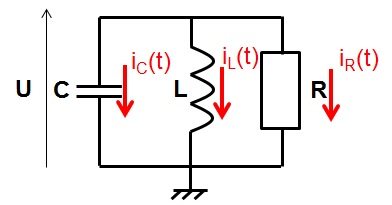
\includegraphics[scale=0.5]{images/circuit_RLC_reponse_naturelle.jpg}
          \end{minipage}
          
          On souhaite déterminer la réponse naturelle de ce circuit pour
          $t > 0$, sous la forme de la tension $u(t)$ mesurée aux bornes du
          circuit. On souhaite aussi déterminer la fréquence naturelle
          de ce circuit, caractérisant sa réponse transitoire.
          
          
          Commençons par appliquer la loi des
          nœuds à ce circuit, qui permet d'écrire :
          $i_{C}(t)+i_{R}(t)+i_{L}(t)=0$. En prenant en compte les
          relations tension-courant pour la résistance et le
          condensateur, cette relation peut être mise sous la forme
          ci-dessous, ne faisant apparaître que le courant. Après
          différenciation de l'équation, on fait apparaître une équation
          différentielle du second ordre. Pour simplifier les notations,
          on pose : $\alpha = \frac{1}{2RC} $ et
          $\omega^{2} = \frac{1}{LC}$.
          \begin{eqnarray*}
            C\dDtDe{u}+\frac{u(t)}{R}+\frac{1}{L}\int u(t) \deriv t=0 \quads\implies\quads \dDtDeOrdre{u}{2}+\frac{1}{RC}\dDtDe{u}+\frac{1}{LC}\,u(t) = 0\\
            \dDtDeOrdre{u}{2} + 2\alpha \dDtDe{u}+\omega^{2}u(t) = 0
          \end{eqnarray*}
          
          On retrouve une équation du même type que
          \ref{eq:reponse_naturelle}. Un vecteur solution de cette
          équation peut donc s'écrire : $u(t) = A\,\expo{pt}$. En intégrant
          cette solution dans l'équation différentielle, on en déduit
          l'équation caractéristique de ce circuit~:
          \begin{eqnarray}
            \label{eq:carac_RLC}
            \forall t\in\R\quads \p{p^{2}+2\alpha p+\omega^{2}}A\expo{pt}=0 \nonumber\\
            \iff  p^{2}+2\alpha p+\omega^{2}=(p-p_{1})(p-p_{2})=0
          \end{eqnarray}
          Cette équation présente deux racines $p_{1}$ et $p_{2}$. Ce
          circuit électrique est donc un système d'ordre 2, dont la
          réponse naturelle va s'écrire :
          \begin{equation}\label{key}
            u(t) = A_{1}\expo{p_{1}t}+A_{2}\expo{p_{2}t}
          \end{equation}
          
          où $A_{1}$ et $A_{2}$ dépendent des conditions
          initiales. Selon la valeur de R, L et C, la nature et la
          position de ces racines dans le plan complexe va changer, modifiant
          le comportement transitoire du circuit. Pour déterminer ces
          racines, il suffit de résoudre une équation d'ordre 2, dont le
          déterminant est donné par :
          $\Delta = 4(\alpha^{2}-\omega^{2})$. La nature des racines
          varie selon le signe du déterminant :
          \begin{equation}
            si~\alpha \geq \omega : \left \{
              \begin{array}{l}
                p_{1}=\frac{-2\alpha +\sqrt{\Delta}}{2}=-\alpha+\sqrt{\alpha^{2}-\omega^{2}} \\
                p_{2}=\frac{-2\alpha -\sqrt{\Delta}}{2}=-\alpha-\sqrt{\alpha^{2}-\omega^{2}} \\
              \end{array}
            \right.
          \end{equation}
          \begin{equation}
            si~\alpha < \omega : \left \{
              \begin{array}{l}
                p_{1}=\frac{-2\alpha +j\sqrt{-\Delta}}{2}=-\alpha+j\sqrt{\omega^{2}-\alpha^{2}} \\
                p_{2}=\frac{-2\alpha -j\sqrt{-\Delta}}{2}=-\alpha-j\sqrt{\omega^{2}-\alpha^{2}} \\
              \end{array}
          \right.
	\end{equation}
	On peut distinguer plusieurs types de comportement transitoire
        distincts selon les valeurs de $\alpha=\frac{1}{2RC}\geq 0$ et $\omega=\frac{1}{\sqrt{LC}\geq 0}$~:
	\begin{itemize}
        \item si $\alpha \neq 0$, alors les deux racines présentent
          une partie réelle négative. Le système présente donc un
          caractère stable.
        \item si $\alpha \geq \omega$, les deux racines sont purement
          réelles et négatives. Dans le plan complexe, elles sont situées sur
          l'axe des réels à gauche de l'axe des imaginaires. La
          réponse du circuit sera du type exponentiel décroissant sans
          oscillation (équivalent au point 2 de la figure
          \ref{Fig:reponse_vs_p}).
        \item si $\alpha < \omega$ et $\alpha \neq 0$, les deux
          racines sont conjuguées. Elles sont situées à gauche de
          l'axe des imaginaires dans le plan complexe. La réponse du circuit
          sera du type oscillation amortie de pulsation
          $\sqrt{\omega^{2}-\alpha^{2}}$ (équivalent au point 4 de la
          figure \ref{Fig:reponse_vs_p}).
        \item si $\alpha = 0$, les deux racines sont purement
          imaginaires et conjuguées. Elles sont placées sur l'axe
          imaginaire du plan complexe, symétriquement à l'axe de réels. La
          réponse du circuit sera une oscillation non amortie de
          pulsation $\omega$ (équivalent au point 1 de la figure
          \ref{Fig:reponse_vs_p}).  Cela correspond au cas 
           $R=0, C\neq 0$ d'une résistance nulle
          entretenant des oscillations perpétuelles (stabilité limite
          ou simple)
	\end{itemize}
      \end{exemple}
	
	\section{Réponse forcée}
	
	La réponse forcée est la solution de l'équation générale du
        système pour une excitation non nulle. La réponse va dépendre
        de la forme de l'excitation, mais aussi des propriétés du
        système. Puisque la réponse dépend de l'excitation, il est
        préférable de déterminer des excitations dont les propriétés
        faciliteront l'analyse de la réponse forcée d'un système. Pour
        cela, il faut chercher des familles d'excitation dont la forme
        n'est pas modifiée par l'effet du système LTI. Ainsi, en
        connaissant la forme de l'excitation, on déduira immédiatement
        la forme de la réponse. Seuls quelques coefficients que nous
        préciserons seront à calculer.
	
	Nous allons nous intéresser à deux familles d'excitations
        répondant à ce critère : l'excitation exponentielle complexe
        (que nous avons rencontré précédemment) et la famille
        d'excitation impulsionnelle.
	
	\subsection{Excitation exponentielle complexe}
	L'excitation exponentielle complexe présente la forme suivante~:
	\begin{equation}\label{eq:exc_expo_complexe}
          x =    \left \{
            \begin{array}{l l}
              \hat{X}  \expo{p_{x}t}  & si~t>0 \\
              0   & sinon \\
            \end{array}
          \right .
	\end{equation}
	
	où $ \hat{X} = |x| \expo{j \theta}$ est l'amplitude complexe,
        ou vecteur de Fresnel, ou le phaseur du signal. Et
        $p_{x} = \alpha +j\,\omega $ sa fréquence complexe. Dans le
        cas où l'on s'intéresse à des signaux réels (cas rencontré en
        pratique), cette forme reste valable à condition de ne
        conserver que la partie réelle. Elle s'écrit alors :
	\begin{equation}\label{eq:exc_expo_complexe_reel}
          x(t) =    \left \{
            \begin{array}{l l}
              \Reel{\hat{X}  \expo{p_{x}t}} = |X|  \expo{\alpha t}  cos(\omega t+\theta)  & si~t>0 \\
              0   & sinon \\
            \end{array}
          \right .
	\end{equation}
	Comme dans le cas de la fréquence naturelle, la fréquence
        complexe peut être représentée dans le plan complexe. Sa position
        indique qualitativement la forme temporelle de
        l'excitation. Si p\textsubscript{x} est purement réelle,
        l'excitation est une fonction exponentielle pure. Si
        p\textsubscript{x} est purement imaginaire, l'excitation est
        une fonction cosinusïdale pure. L'excitation est dite
        monochromatique. |X| représente son amplitude et $\theta$ sa
        phase.
	
        \begin{exemple} Récrivez les expressions des fonctions
          ci-dessous sous la forme de fonctions réelles :
          $y(t)=Re[(1+j)\expo{(-2+j)t}]$ et
          $z(t) = Re[2\expo{j\frac{\pi}{2}}\expo{j10t}]$.Les deux
          fonctions sont des exponentielles complexes. Elles
          représentent des signaux temporels réels puisqu'on ne
          conserve que la partie réelle.

          Le phaseur de la fonction
          $y(t)$ peut s'écrire
          $\hat{Y}=1+j=\sqrt{2}\expo{j\frac{\pi}{4}}$. La fréquence
          complexe est $p_y=-2+j$. Elle contient une partie réelle
          négative donnant un comportement d'exponentielle
          décroissante de constante de temps $2$ à l'amplitude, et une
          partie imaginaire donnant un comportement oscillant de
          pulsation égale à $1$. La fonction $y(t)$ peut donc s'écrire~:
          \[y(t)={\sqrt{2}}\expo{-2t}cos(t+\frac{\pi}{4})\]

          En procédant de même pour la fonction $z(t)$, on remarque
          que sa fréquence est purement complexe de pulsation 10, son
          phaseur est d'amplitude $2$ et de phase $\frac{\pi}{2}$. Il
          s'agit d'une fonction cosinusoïdale s'écrivant :
          $z(t)=2\,cos(10\,t+\frac{\pi}{2})$.
      \end{exemple}
	
	
      L'excitation exponentielle complexe a une propriété remarquable
      : l'action d'un opérateur linéaire (proportionnel, intégrateur
      ou différentiel) laisse sa forme inchangée. Seule son amplitude
      complexe (phaseur) sont modifiées. On peut donc en déduire une
      propriété des systèmes LTI~: lorsqu'un système linéaire est
      excité par un signal exponentiel complexe (en pratique, un
      signal sinusoïdal), la réponse sera aussi une fonction du même
      type et de même fréquence complexe. Seule l'amplitude et la
      phase changeront. Cette propriété en fait un signal d'analyse
      intéressant.
	
      \subsection{Famille d'excitations impulsionnelles}
	
	Nous parlons ici de familles car nous allons parler de
        plusieurs fonctions, reliées entre elles et associées à une
        excitation très importante dans l'analyse des systèmes et des
        signaux : l'impulsion de \Dirac.
	
	\subsubsection{Echelon unitaire ou fonction de Heaviside}

        L'échelon unitaire\footnote{Nommée \emph{step function}
          outre-manche} ou fonction de \Heaviside{} représente le
        signal que l'on obtiendrait derrière un interrupteur idéal que
        l'on fermerait à $t = 0$, et modélise le fait que l'on ne
        s'intéresse pas à ce qui c'est passé avant l'instant $t=0$.
        \begin{definition}{Échelon unité ou de \Heaviside{}}

          On note $u$ la \emph{fonction échelon}, ou \emph{fonction de
            \Heaviside{}}, la fonction définie par~:\newline
	\begin{minipage}[l]{0.4\linewidth}
          \begin{equation}
          \label{eq:heaviside}
          u : t \mapsto \left \{
            \begin{array}{l l}
              1  & \text{si }t>0 \\
              0   & \text{si }t<0 
            \end{array}
          \right .	 	
	\end{equation}
	\end{minipage}\hfill
	\begin{minipage}[r]{0.55\textwidth}
          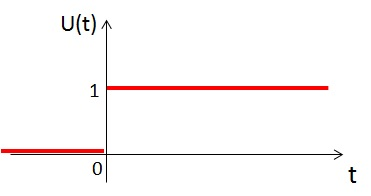
\includegraphics[width=0.9\linewidth]{images/Heaviside.jpg}
	\end{minipage}
      \end{definition}
      \begin{remarque}
        Selon l'utilisation voulue, cette fonction peut être définie
        en 0 par prolongement continu à gauche ($u(0)=0$) ou à droite
        ($u(0)=1$), ou de manière discontinue (par exemple
        $u(0)=\frac{1}{2}$ pour respecter le théorème de \Dirichlet{}
        avec les séries de \Fourier{}). On peut aussi simplement laisser
        cette fonction définie seulement sur $\R^{\star}$.
      \end{remarque}
        
      À l'aide de cette fonction, on peut définir la \emph{fonction
        porte}\footnote{On dit \emph{boxcar function} chez les saxons}, ou bien
      encore \emph{fenêtre naturelle} voire parfois \emph{fonction
        rectangle}, pour représenter le fait que l'on s'intéresse à un
      signal dans une fenêtre temporelle donnée.
        
      \begin{definition}{Fonction porte ou fenêtre naturelle}

        On note $\porteDe{a}{b}$ la fonction définie par:
        \begin{equation}
          \label{eq:porte}
          \porteDe{a}{b} \quads= t \mapsto u\de{t-a}-u\de{t-b} \quads= t\mapsto \pparMorceaux{1}{\text{si } a<t<b}{0}{\text{si } t<a \text{ ou } t>b} 
        \end{equation}

        On note $\porte$ la fonction porte unitaire définie par~:
\begin{equation}
          \label{eq:porte_unitaire}
          \Pi \quads= \porteDe{-\frac{1}{2}}{\frac{1}{2}} \quads= t\mapsto \pparMorceaux{1}{\text{si } t<\abs{1/2}}{0}{\text{si } t>\abs{1/2}} 
        \end{equation}   
      \end{definition}

      Cette fonction peut être utilisée pour approcher n'importe
      quelle autre fonction par une fonction en marches d'escalier de largeur $\Delta_\tau$ avec la forme~:
      \begin{equation}
        \label{eq:escalier}
        t\mapsto f(t)  \approx t\mapsto \sum_{k\in\Z} f\de{k\Delta_\tau}\,.\,\porteDe{0}{\Delta_\tau}\de{t-k\Delta_\tau}
      \end{equation}
      Ce type de fonction escalier est utilisé dans la définition de
      l'intégrale au sens de \grandPonte{Riemann} que l'on peut
      ré-écrire~:
      \begin{equation}
        \label{eq:integrale_escalier}
        \int\limits_{a}^{b}f(t)\,\deriv t = \lim_{\Delta\tau \to 0} \sum_{k\in\Z} \porteDe{a}{b}\de{k\Delta_\tau} \; f\de{k\Delta_\tau}\;\underbrace{\Delta_\tau}_{=\int\limits_\R\porteDe{0}{\Delta_\tau}\de{t-k\Delta_\tau}}
      \end{equation}
      où vous remarquez l'utilisation de la fonction porte $\porteDe{a}{b}$ pour annuler la fonction à intégrer en dehors des bornes fixées.

      \begin{exemple}
        Prenons une fonction en dent de scie définie par morceaux dont
        vous pouvez compléter le graphe sur la
        \figref{fig:approx_escalier} à partir de la définition
        suivante~:
        \begin{equation*}
         x : t \mapsto \ppparMorceaux
          {t+1}{\text{si } t\in\left[-1 ; 1\right[}
          {2}{\text{si }t\in\left[1 ; 2\right[}
          {0}{\text{sinon}}
          \iff x = \porteDe{-1}{1}.\p{\Id+\uniteDe{L_E}}+\porteDe{1}{2}.2\,\uniteDe{L_E}
        \end{equation*}
        comme $x$ est continue à droite, remarquez que la fonction
        porte $\porteDe{-1}{1}$ est considérée avec son prolongement à
        droite pour définir le support $\left[-1 ; 1\right[$ où la
        fonction $\Id+\uniteDe{L_E}=t\mapsto t+1$ doit être
        considérée. Une autre fonction porte est utilisée pour définir
        le support de la fonction constante
        $2\,\uniteDe{L_E}=t\mapsto 2$ et la fonction est donc laissée
        nulle ailleurs (y compris en $t=2$ puisque continue à droite).
        \begin{figure}[htbp]
          \centering
          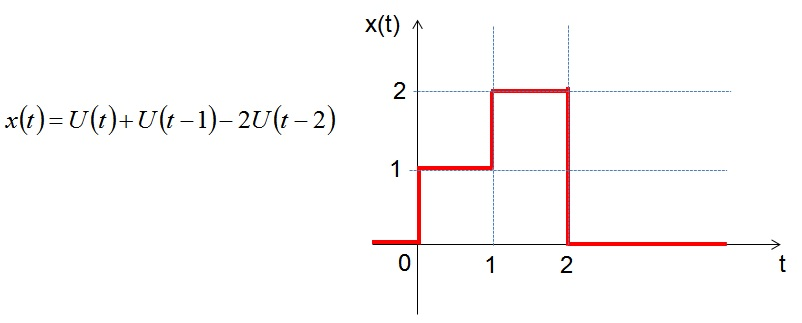
\includegraphics[scale=0.5]{images/Utilisation_Heaviside.jpg}
          \caption{Exemple d'utilisation de la fonction de Heaviside
            pour bâtir une fonction plus complexe}
          \label{fig:approx_escalier}
	\end{figure}

        Si nous approchons cette fonction en utilisant 
        \eqref{eq:escalier} avec un pas d'échantillonage
        $\Delta_\tau=1$, seuls les deux échantillons $x(0)=1$ et
        $x(1)=2$ sont non nuls et on obtient l'approximation en deux
        fonctions portes non nulles (en rouge sur
        la~\figref{fig:approx_escalier})~: ~:
        \begin{equation*}
          \forall t\in\R\quads x(t)\approx \porteDe{0}{1}\de{t}+2\porteDe{1}{2}\de{t} = \underbrace{\porte\de{t-\frac{1}{2}}}_{\text{vaut 1 autour de }0,5}+\underbrace{2\,\porte\de{t-\frac{3}{2}}}_{\text{vaut 2 autour de }1,5}
        \end{equation*}
        En remplaçant les fonctions portes par leur composition en
        fonctions de \Heaviside{}, on obtient une approximation en 3
        échelons dont l'amplitude représente le saut relatif à
        effectuer pour passer d'un escalier à un autre~:
        \begin{equation*}
          x(t) \approx \underbrace{u(t)}_{+1\text{ à }t=0} + \underbrace{u(t-1)}_{+1\text{ à }t=1} +\underbrace{ -2\,u(t)}_{-2\text{ à }t=2}
        \end{equation*}

        Cela permet d'approcher la valeur de l'intégrale de $x(t)$
        en utilisant \eqref{eq:integrale_escalier} pour avoir~:
        \begin{eqnarray*}
          &\intDt{\R}{}{x\de{t}}=\intDt{_1}{2}{x(t)}=\underbrace{\intDt{-1}{1}{t+1}}_{=2}+\underbrace{\intDt{1}{2}{2}}_{=1} = 3 \\
          \approx  &\somme{k\in\Z}{}{\porteDe{-1}{2}\p{k\Delta_\tau}x\p{k\Delta_\tau}}\Delta_\tau =  \somme{k=-1}{2}{x(k)} = \caCest{x(-1)}{=0} + \caCest{x(0)}{=1} + \caCest{x(1)}{=2} + \caCest{x(2)}{=0} = 3
        \end{eqnarray*} 
      \end{exemple}
      
      La fonction de \Heaviside{} peut servir de base pour générer
      d'autres fonctions de type causal, par intégration ou
      différenciation. Par exemple, en l'intégrant une fois, on
      obtient la \emph{fonction rampe}\footnote{appelée \emph{ramp
          function} de manière assez similaire dans les pays où l'on
        roule pourtant à gauche.} $t\mapsto t\,u(t)$. Si on l'intègre
      $n$ fois, on obtient la base des fonctions polynomiales
      causales, \cad{} nulles pour $t<0$.
	\begin{equation}\label{eq:integration_Heaviside}
          u^{(-n)}(t) = \frac{t^{n}}{!n}  u(t)	 	
	\end{equation}	où $u^{\p{n}}$ désigne la n\ieme{} dérivée et par extension $u^{\p{-n}}$ la n\ieme{} primitive qui s'annule en $0$.
        
	Le cas de la dérivation est plus complexe car elle entraîne
        l'apparition d'une discontinuité. En effet, la dérivée de la
        fonction de \Heaviside{} n'est pas définie en $0$ car non
        continue en $0$. Cet écueil ne peut se traiter qu'en utilisant
        la théorie des distributions, qui va permettre de définir
        l'impulsion de \Dirac.
	
	\subsubsection{Impulsion ou distribution de \Dirac}
	
	L'impulsion de \Dirac{} se trouve, par exemple, en
        différenciant l'échelon unitaire. On voit immédiatement
        apparaître un problème : la dérivée est nulle presque partout,
        sauf au point 0 où l'échelon présente une discontinuité et où
        sa dérivée est infinie. Au sens classique des fonctions la
        dérivée de l'échelon unité est la fonction nulle, car on ne
        peut que proposer un prolongement continu en $0$ qui vaut $0$
        pour pourvoir l'intégrer et l'intégrale devient alors nulle~!

        \begin{remarque}
          Dans l'espace des fonctions continues $\classeZero$, les
          applications (ou opérateurs puisque l'application transforme
          une fonction en une fonction) dérivée et intégrale
          sont réciproques. Ces applications sont bijectives et ont un
          noyau nul car seul la fonction nulle $\nullDe{\classeZero}$
          à pour dérivée la fonction nulle.

          En revanche dans l'espace des signaux physiques $L_E$
          considéré, pouvant donc être discontinus, on voit que au
          moins $u(t)$ et $\nullDe{L_E}$ ont pour dérivée la fonction
          nulle. Le noyau de l'application dérivée n'est plus réduit à
          $\{\nullDe{L_E}\}$ mais est au moins de dimension $1$
          puisque $\vect{u} \subset \ker{\dDtDe{}}$. Les opérateurs
          dérivée et intégrale ne sont plus réciproque.
        \end{remarque}
        
        Pourtant l'intuition physique nous pousse à penser qu'intégrer
        la dérivée d'un échelon doit redonner un échelon et qu'il
        existe bien un signal qui, donné en entrée d'un intégrateur,
        provoque un échelon en sortie. De même lorsque l'on considère
        une particule élémentaire comme une masse ponctuelle à travers
        une fonction de densité de masse, on introduit une fonction
        nulle partout sauf au point où se trouve la particule et dont
        la valeur de densité de masse est infinie, cependant sont
        l'intégrale vaut la masse de la particule. C'est pour cela que
        \Dirac{} introduit la \emph{fonction Delta} dans le
        développement de la théorie quantique des champs sans pour
        autant en donner une définition mathématique valable. Cette
        fonction apparaît aussi lorsque l'on considère la fonction de
        densité de probabilité $p(x)$ d'un événement discret tel qu'un
        jet de dé~: la densité de probabilité en dehors des nombres
        entier est nulle mais infinie pour chaque valeur de $1$ à
        $6$. Pourtant lorsque l'on veut la probabilité de tirer $1$
        sur un jet, on intègre cette densité autour de $1$ et l'on veut
        obtenir
        $\int\limits_{1-\epsilon}^{1+\epsilon}p(x) \deriv x=\frac{1}{6}$

        Il
        faudra, 30 ans plus tard, deux médailles Field et bâtir la
        théorie des \emph{Distributions} ou des \emph{fonctions
          généralisées} pour en donner une définition correcte et
        obtenir une généralisation de la notion de fonction permettant
        de dériver les fonctions non--continues en tout points~!

        Le but de cette partie n'est pas de faire une présentation
        exhaustive de la théorie des distributions, mais de donner du
        sens à cette impulsion de \Dirac, de décrire comment
        l'utiliser convenablement et de lui donner une place centrale
        dans l'études des systèmes et des signaux.

        Il est possible de donner une justification physique à
        l'impulsion de \Dirac{} par un passage à la limite, comme
        illustrée sur la figure ci-contre. On considère une fonction
        échelon avec un temps de transition finie $\tau$. En dérivant
        cette fonction, on obtient une fonction décrivant une
        impulsion brève de durée $\tau$. L'aire de cette fonction,
        associée à son intégrale sur $\R$, est égale à 1 quel que soit
        $\tau$. Par passage à la limite quand $\tau$ tends vers 0, on
        se rapproche d'une fonction nulle presque partout sauf en $0$
        où elle tend vars l'infini et dont l'intégrale vaut
        $1$. L'impulsion de \Dirac{} peut être présentée comme un
        algorithme de passage à la limite d'une impulsion, elle est
        donc décrite par \og{} son effet sous l'intégrale \fg{} et
        n'admet pas de définition classique même en tant que limite de
        fonction~:
	
        \begin{figure}[htbp]
          \begin{minipage}[l]{0.4\linewidth}
          \begin{equation}\label{Dirac_aire}
            \int_{\mathbb{R}}\delta (t)dt = 1 	
          \end{equation}
	\begin{equation}\label{Dirac_derive}
          \delta (t) = \frac{du(t)}{dt}	 	
	\end{equation}
	\end{minipage} \hfill
	\begin{minipage}[r]{0.6\linewidth}
          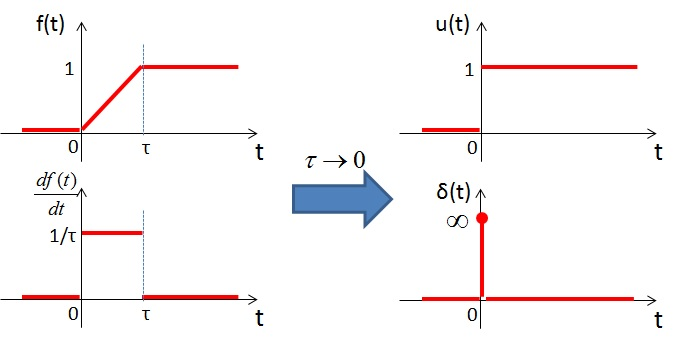
\includegraphics[scale=0.5]{images/generation_Dirac.jpg}
   	\end{minipage}
	\vspace{0.5\baselineskip}
        
        \caption{Le \Dirac{} vu par le passage à la limite d'une
          fonction continue. Attention la limite de l'impulsion
          continue lorsque $\tau\to 0$ est toujours la fonction
          nulle presque partout et non pas un \Dirac{}. Cependant son
          effet sous l'intégrale n'est pas celui de la fonction
          nulle.}
        \label{fig:dirac}
      \end{figure}
	L'impulsion de \Dirac{} est donc un objet mathématique qui
        n'est pas une fonction classique, on parle de fonction
        généralisée, qui est une dérivée non nulle de l'échelon et
        dont l'intégrale est la fonction échelon. 

        La position de cette impulsion n'est pas forcément centré en
        0. On notera $\delta_a$ la fonction généralisée dont
        l'intégrale est l'échelon centré en $a$ soit
        $u_a : t\mapsto u\p{t-a}$ et donc la fonction Delta est par
      défaut $\delta = \delta_0$. Il n'est pas rare de voir la
      fonction généralisé Delta utilisée et nommée comme une fonction
      classique, par exemple \og{} la fonction $\delta(t-a)$ \fg{} au
      lieu de la distribution $\delta_a$. Ce sont des abus de langage
      avec lesquels il faut être prudent car si certaines propriétés
      (comme ici le décalage dans le temps et donc la composition avec
      une fonction $t\mapsto t-a$ ) sont conservée par les
      distributions, d'autre ne le sont pas.
        
	% TODO ça c'est faux ! l'impulsion est infinie en 0 !
        % De manière générale, on peut écrire que la distribution ou
        %impulsion de \Dirac{} est définie par l'équation \ref{Dirac}.
	% \begin{equation}\label{Dirac}
        %   \delta (t-a) = \left \{
        %     \begin{array}{l}
        %       1~~~si~t = a \\
        %       0~~~sinon \\
        %     \end{array}
        %   \right . 	
	% \end{equation}

      %TODO pas compris pourquoi If(delta) et pas If(t0)...
	Quel peut être l'intérêt d'un tel objet mathématique, nul
        partout sauf en un point où il devient infini ? Il est certain
        qu'il ne peut être utilisé comme une fonction. Par contre, il
        peut servir à calculer une fonction indicatrice
        $I_{f}(t_0)$ pour mesurer une caractéristique d'une
        fonction f, définie en $\mathbb{R}$, autour de l'instant$t_0$.
        Comme le montre \eqref{eq:fonction_indicatrice}. La fonction $f$ est
        localement intégrable et $\delta(t)$ sert de fonction de mesure~:
	\begin{equation}\label{eq:fonction_indicatrice}
          I_{f}(t_0)=\int_{\mathbb{R}}\delta(t-t_0)f(t)dt
	\end{equation}
	
	À l'intérieur de l'intégrale, la distribution de \Dirac{}
        prend tout son sens, car elle est définie par son effet sous
        l'intégrale. Elle va permettre de mesurer la fonction f au
        point $t = t_0$. En effet, à l'intérieur de l'intégrale, en
        multipliant l'impulsion avec la fonction $f$ et en l'intégrant
        sur un intervalle infiniment court, on prélève la valeur de
        la fonction f au point $t = t_0$. On appelle cette propriété
        la propriété d'échantillonnage, donnée par
        \eqref{eq:dirac_echantillonage}. Celle-ci présente un très grand
        intérêt dans l'étude des signaux.
	
	 \begin{eqnarray}\label{eq:dirac_echantillonage}
           \int_{-\infty}^{+\infty} \delta\p{t}  f(t) \deriv t  = f(0)  \\ 
           \int_{-\infty}^{+\infty} \delta_{t_0}\, f(t) \deriv t  = f(t_0) \nonumber 
	 \end{eqnarray}
	
	Précisons-le à nouveau : l'utilisation de l'impulsion de
        \Dirac{} n'a de sens qu'à l'intérieur d'une intégrale. Ce n'est
        pas une fonction classique mais une distribution ou fonction
        généralisée. L'usage pratique montre qu'on trouve souvent
        l'impulsion de \Dirac{} utilisée à l'extérieur de toute
        intégrale, comme une fonction mathématique classique. C'est
        bien entendu une écriture abusive et potentiellement source
        d'erreur. Cependant, ce type d'écriture permet parfois une
        simplification de l'écriture des calculs, qui est toléré si
        l'impulsion de \Dirac{} est correctement employée dans une
        intégrale. Il est courant de représenter sur un graphique
        l'impulsion de \Dirac, au même titre qu'une
        fonction. Techniquement, c'est impossible car l'amplitude de
        l'impulsion de \Dirac{} devient infinie. Par convention, on la
        représente sous la forme d'un trait, terminé par une flèche,
        avec à proximité une valeur placée entre parenthèse indiquant
        l'aire du \Dirac, \cad{} l'amplitude de l'échelon obtenu par
        intégration. Cette aire est appelé \emph{poids} du \Dirac{} en
        référence à son utilisation dans les fonction densité de masse
        dont l'intégrale donne le poids de la particule.

        La figure \ref{fig:representation_dirac} illustre cette
        représentation, avec l'affichage de l'impulsion
        $2\delta_1$.
        \begin{figure}[htbp]
          \centering
          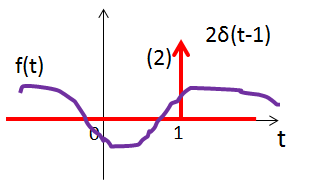
\includegraphics[scale=0.6]{images/representation_Dirac.png}
          \caption{Représentation graphique conventionnelle d'une
            impulsion de \Dirac de poids 2 et centrée en 1. Remarquez
            la notation abusive $\delta\p{t-1}$ au lieu de $\delta_1$}
          \label{fig:representation_dirac}
	\end{figure}
L'impulsion est centrée en t = 1 et son poids
        est égal à 2. Sur ce graphe, on a superposé l'impulsion de
        \Dirac{} avec le tracé d'une fonction $f$
        quelconque. L'utilisation de l'impulsion à l'intérieur de
        l'intégrale \ref{Dirac_echantillonage_2} permet d'extraire la
        valeur de f au point $t = 1$.


        Revenons au problème initial de sélection de familles
        d'excitation inchangées par l'effet d'un système LTI. On peut
        remarquer que cette propriété est aussi vérifiée avec la
        famille d'excitation impulsionnelle. L'action d'un opérateur
        proportionnel, intégrateur ou dérivée appliquée à une fonction
        de cette famille donnera une nouvelle fonction appartenant
        aussi à cette famille. De plus, on comprend intuitivement
        l'intérêt de l'impulsion de \Dirac{} pour déterminer la
        réponse temporelle d'un système à n'importe quelle
        excitation. De par sa propriété d'échantillonnage, chaque
        point d'une excitation peut être modélisée, à la limite, par
        une impulsion de \Dirac. L'excitation complète peut donc être
        modélisée comme la superposition d'un nombre infini
        d'impulsions de \Dirac. Si on sait comment le système réagit à
        une impulsion de \Dirac, la réponse à l'excitation sera la
        superposition des réponses à toutes les impulsions de \Dirac,
        puisque le système est linéaire.
	
	
	
	\section{Les différents types de réponse caractérisant les systèmes LTI}
	Maintenant que nous avons défini deux familles d'excitation
        adaptées à l'étude des systèmes LTI, nous pouvons définir
        plusieurs types de réponse qui nous aideront à analyser les
        propriétés de ces systèmes.
		
	
	\subsection{Réponse impulsionnelle}
	Elle correspond à la réponse d'un système excité par une
        impulsion de \Dirac, cette réponse est notée $h(t)$~:
        % TODODONE : faux pas son énergie, mais son poids et confusion
        % avec amplitude.
        % Même si l'amplitude de cette impulsion est infinie, son
        % énergie vaut 1.
        % Au lieu de
        % représenter cette valeur infinie, nous utiliserons la valeur
        % de 1. N'oublions pas qu'il ne s'agit pas d'une fonction mais
        % d'une distribution, qui n'a du sens qu'à l'intérieur d'une
        % intégrale.
	\begin{equation}
          h = L\b{\delta_0}
        \end{equation}
	Quel que soit le système LTI considéré, puisque l'excitation
        devient nulle pour t > 0, on retrouve le calcul de la réponse
        naturelle. L'application de l'impulsion en t=0 ne fait que
        changer les conditions initiales.
	
	\begin{equation}\label{}
          si~x(t)=\delta (t)~\rightarrow ~y_{f}(t) = y_{0}(t)	 	
	\end{equation}
	
	
	
	\vspace{1\baselineskip} La réponse impulsionnelle va nous
        fournir un moyen de calculer la réponse d'un système LTI à
        n'importe quelle excitation, en effectuant les calculs
        uniquement dans le domaine temporel. C'est ce que nous allons
        démontrer. Tout signal peut être vu comme la superposition
        d'un nombre infini de points, pouvant être modélisés par des
        impulsions de \Dirac, pondérées et décalées dans le
        temps. Comme le montre la figure
        \ref{Fig:Approx_excitation_Dirac}, une excitation quelconque
        x(t) peut être approximée par une suite de rectangles
        adjacents, de largeur $ \Delta_\tau $, que l'on peut remplacer
        par des impulsions de \Dirac{} équivalentes de même
        surface. Ainsi, elles transportent la même énergie. Si la
        largeur $ \Delta_\tau $ tend vers zéro, cette approximation
        devient de plus en plus juste. Dans l'exemple considéré, on
        suppose que x(t) = 0 pour t \textless{} 0 par souci de
        lisibilité. Le même raisonnement resterait juste avec x(t) non
        nul pour t \textless{} 0. L'excitation peut alors s'approximer
        par :
	
	
	\begin{equation*}\label{}
          \sum_{n=-\infty}^{+\infty}x(n\Delta_\tau) 	\Delta_\tau  \delta (t-n\Delta_\tau)	
	\end{equation*}
	
	\begin{figure}[htbp]
          \centering
          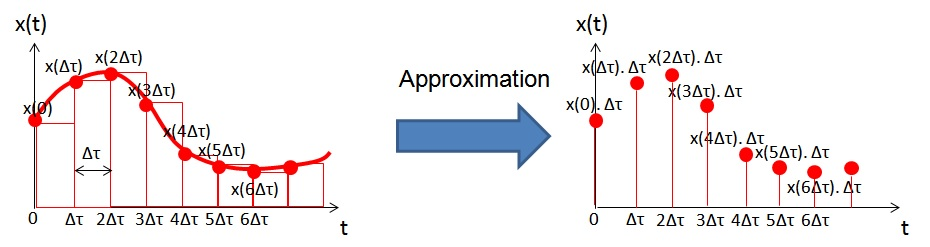
\includegraphics[scale=0.5]{images/Approx_excitation_Dirac.jpg}
          \caption{Excitation quelconque x(t) approximée par une suite
            d'impulsion de \Dirac}
          \label{Fig:Approx_excitation_Dirac}
	\end{figure}
	Supposons que cette excitation attaque l'entrée d'un système
        LTI dont la réponse impulsionnelle h(t) est connue
        (Fig. \ref{Fig:reponse_impuls_illustration}). Par souci de
        lisibilité, on suppose aussi que h(t) = 0 pour t < 0.
	\begin{figure}[htbp]
          \centering
          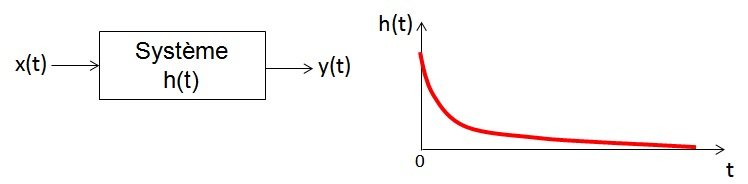
\includegraphics[scale=0.5]{images/reponse_impuls_illustration.jpg}
          \caption{Réponse impulsionnelle d'un système}
          \label{Fig:reponse_impuls_illustration}
	\end{figure}
	
	Chaque impulsion élémentaire composant x(t) et apparaissant à
        l'instant $ k \times \Delta_\tau $ contribue à la réponse en
        sortie, comme l'illustre la figure
        \ref{Fig:illustration_reponse_impuls_2}. Chacune d'entre elles
        produit une réponse égale à la réponse impulsionnelle du
        système, mais :
	
	\begin{itemize}
        \item pondérée par l'amplitude de l'excitation d'entrée à
          l'instant $ k \times \Delta_\tau $
	
        \item décalée dans le temps de $ k \times \Delta_\tau $~
	\end{itemize}
	\begin{figure}[htbp]
          \centering
          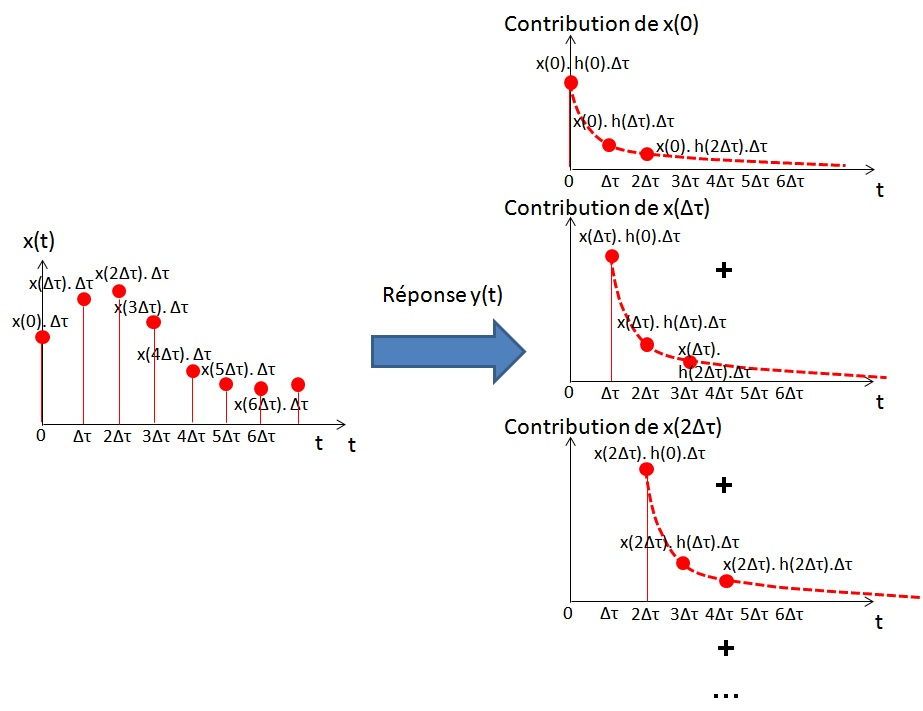
\includegraphics[scale=0.5]{images/illustration_reponse_impuls.jpg}
	\end{figure}
	\begin{figure}[htbp]
          \centering
          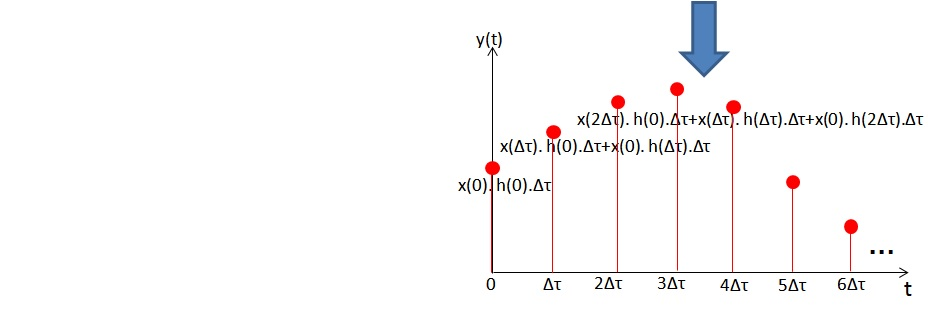
\includegraphics[scale=0.6]{images/illustration_reponse_impuls_2.jpg}
          \caption{Construction de la réponse impulsionnelle}
          \label{Fig:illustration_reponse_impuls_2}
	\end{figure}

	La réponse globale du système est obtenue en sommant
        l'ensemble des contributions de chaque impulsion élémentaire
        formant l'excitation. Elle peut alors s'approximer par :
	\begin{equation*}\label{key}
          \sum_{n=-\infty}^{+\infty} x\p{n\Delta_\tau}  \Delta_\tau  h(t-n\Delta_\tau)
	\end{equation*}
	
	En faisant tendre $ \Delta_\tau $ vers zéro, cette somme
        converge vers une intégrale donnée par la relation
        ci-dessous. Ce calcul intégral particulier, faisant intervenir
        le produit de deux fonctions dont les indices $\tau $ et
        $t-\tau $ sont balayés dans des directions opposées, porte un
        nom : le produit de convolution. Cette opération est
        symbolisée par le signe $*$.
	\begin{equation}\label{Demo_produit_convolution}
          y(t) = \lim_{\Delta_\tau \to 0} \somme{n=-\infty}{+\infty}{x\de{n\Delta_\tau}}  \;  h\de{t-n\Delta_\tau}\;\Delta_\tau = \intDt{-\infty}{+\infty}{x\de{\tau}\, h\de{t-\tau}} = x*h(t)
	\end{equation}
	
	Cette relation basée sur le produit de convolution fournit
        donc un outil de calcul de la réponse du système directement
        dans le domaine temporel. Cependant, c'est un calcul complexe,
        passant par une opération longue et fastidieuse si elle est
        effectuée à la main. Nous y reviendrons au chapitre 7, qui
        sera consacré au calcul des réponses des systèmes LTI
        directement dans le domaine temporel. Cependant, avant
        d'aborder ce point, nous allons d'abord considérer le cas
        d'une excitation exponentielle complexe pour dériver le
        concept de fonction de transfert défini dans le domaine
        fréquentiel. Nous verrons que dans ce domaine, le calcul de la
        réponse du système est beaucoup plus aisée !
	
	\subsubsection{Condition pour garantir la causalité}
	Un système est causal si sa réponse ne dépend que des états
        passés et présents. A partir de la réponse impulsionnelle, on
        peut en déduire une condition : il faut que h(t) = 0 pour t <
        0. Les systèmes causaux sont les seuls à être physiquement
        réalisables. Le calcul de la réponse d'un système causal à
        partir de sa réponse impulsionnelle peut s'écrire :
	\begin{equation}\label{}
          y(t) = \int_{0}^{+ \infty} x(\tau)  h(t-\tau)d\tau = x*h(t)
	\end{equation}
	\vspace{1\baselineskip}
	
	\subsection{Réponse indicielle}
	Elle correspond à la réponse d'un système excité par une
        fonction de Heavisde. On la note a(t).
	\begin{equation}\label{key}
          si~x(t)=u(t)~\rightarrow ~y_{f}(t)=a(t)
	\end{equation}

	\vspace{0.5\baselineskip}
	
	\textbf{\underline{Autre manière de déterminer la réponse
            impulsionnelle}}
	
	Sans démonstration, on peut affirmer que si on différencie
        l'excitation, on peut déterminer la nouvelle réponse en
        différenciant la réponse à l'excitation initiale : si
        $y(t) = L[x(t)]$ alors $\frac{dy}{dt} = L[\frac{dx}{dt}] $.
        Ainsi, puisque l'impulsion de \Dirac{} est la dérivée de
        l'échelon unitaire, si on connait la réponse indicielle, on
        peut retrouver la réponse impulsionnelle en dérivant la
        réponse indicielle.
	
	\begin{equation}\label{key}
          \delta(t)=\frac{da(t)}{dt}
	\end{equation}
	
	\vspace{0.5\baselineskip}
	
	
	\subsection{Réponse à une exponentielle complexe - Fonction de transfert}
	On considère une excitation exponentielle complexe. La réponse
        forcée a donc la même forme que l'excitation, et présente la
        même fréquence complexe. La seule inconnue est le phaseur
        $\hat{Y}$ de la réponse. Soit l'excitation
        $ x(t) = Re[\hat{X}  \expo{pt}]$ et la réponse
        $ y_{f}(t) = Re[\hat{Y}  \expo{pt}]$ pour t > 0. Si on
        reprend l'équation différentielle ordinaire générale d'un
        système LTI donnée par \ref{eq:generale_lti}, on peut
        écrire la relation suivante.
	
	\begin{equation*}\label{}
          \sum a_{i}  Re[p^{i}  \hat{Y}  \expo{pt}] = \sum b_{i}  Re[p^{j}  \hat{X}  \expo{pt}]
	\end{equation*}
	\begin{equation*}\label{}
          \sum a_{i}  Re[p^{i}  \hat{Y}] = \sum b_{i}  Re[p^{j}  \hat{X}]
	\end{equation*}
	\begin{equation*}\label{}
          \hat{Y}  \sum a_{i}  Re[p^{i}] = \hat{X}  \sum b_{i}  Re[p^{j}]
	\end{equation*}
	
	On peut donc facilement déterminer le phaseur $\hat{Y}$
        associée à la réponse, c'est-à-dire le module et le déphasage
        de la réponse.  On peut alors caractériser l'effet du système
        à une excitation exponentielle complexe quelconque sous une
        forme appelée fonction de transfert, définie comme le rapport
        entre les phaseurs de réponse et d'excitation, et défini pour
        toutes les fréquences complexes.
	\begin{equation}\label{Def_fonction_tranfert}
          H(p) = \frac{Y}{X} (p) = \frac{\hat Y}{\hat X} (p)= \frac{\sum a_{i}  Re[p^{i}]}{\sum b_{i}  Re[p^{j}]}=G\frac{\prod_{i=1}^{M} (p-p_{i})}{\prod_{j=1}^{N} (p-p_{j})}
	\end{equation}
	De manière générale, l'équation \ref{Def_fonction_tranfert} peut s'écrire comme une fraction rationnelle entre deux polynômes, où G est un terme constant. Les N racines du dénominateur sont les pôles de la fonction de transfert et les M racines du numérateur sont appelées les zéros de la fonction de transfert. Comme leur nom l'indique, ils annulent la fonction de transfert lorsque la fréquence $p=p_{j}$. Les pôles sont les mêmes que ceux identifiés dans la réponse naturelle ! Ils ont un rôle prépondérant sur la stabilité du système et la nature de la réponse. Les outils permettant d'étudier l'influence des pôles et des zéros sur la réponse d'un système sortent du cadre de ce cours et seront abordés dans les cours d'automatique.\\
	
	Avec une excitation exponentielle complexe, l'action du
        système LTI peut donc se résumer à la multiplication de
        l'excitation par la fonction de transfert.  On peut souligner
        la facilité de la méthode. Une fois la fonction de transfert
        connue à une fréquence complexe donnée, la réponse forcée à
        une exponentielle complexe de même fréquence est trouvée en
        multipliant le phaseur d'entrée par la fonction de transfert
        (\ref{Relation_Entree_Sortie_Fonction_Transfert}).
	\begin{equation}\label{Relation_Entree_Sortie_Fonction_Transfert}
          \hat{Y}(p) = H(p) \hat{X}(p)=|H(p)||X(p)|\expo{j(arg(H(p))+arg(\hat{X}(p)))}	
	\end{equation}
	
	\vspace{1\baselineskip}
	
	
	\textbf{\underline{Réponse en régime permanent :} }
	
	Dans le cas général, l'excitation est complexe. Le cas
        particulier où $\sigma$ = 0 correspond au cas d'une excitation
        dite monochromatique ou harmonique. On parlera alors de
        réponse en fréquence. Il correspond aussi au cas du régime
        permanent avec $\sigma$ < 0, c'est-à-dire que t devient
        suffisamment grand pour que l'influence du terme
        $\expo{\sigma t}$ devienne négligeable.  La réponse du système se
        trouve facilement en remplaçant la fréquence complexe p par
        $j\omega$. En considérant une excitation cosinusoïdale
        d'amplitude égale à X et de phase $\Phi_{x}$, la réponse du
        système est donnée par la relation suivante.
	
	\begin{equation}\label{calcul_reponse_fonction_transfert}
          y(t) = Re[|H(\omega)|X e^{j(\omega t+arg(H(p))+\Phi_{x})}] =|H(\omega)|X cos(\omega t+arg(H(p))+\Phi_{x})
	\end{equation}
	
	La réponse est une grandeur complexe. Le module de la réponse
        en fréquence est le gain en amplitude de la fonction de
        transfert du système ou du filtre. Le déphasage du signal en
        sortie du filtre par rapport au signal d'entrée est l'argument
        de la fonction de transfert. Le module et la phase sont des
        fonctions de la pulsation $\omega$.
	
	
	\subsubsection{Exemple}
	
	\begin{minipage}[l]{0.7\linewidth}
          On reprend l'exemple du circuit RC abordé dans la partie
          IV.4. On considère toujours que le condensateur est chargé
          initialement en t = 0, avec une tension à ses bornes notée
          $U_C0$. Le circuit est excité par un signal délivrant une
          excitation exponentielle complexe $U_{E}(t)=Xe^{pt}$ avec t
          > 0 et X l'amplitude complexe. La réponse du circuit
          correspond à la tension mesurée aux bornes de la résistance
          R ou tension de sortie. Déterminez la fonction de transfert
          de ce circuit. Indiquez quels sont les pôles et les
          zéros. Quelle est la réponse à un signal cosinuoïdal,
          d'amplitude unitaire et de phase nulle ?
	\end{minipage} \hfill
	\begin{minipage}[r]{0.4\linewidth}
          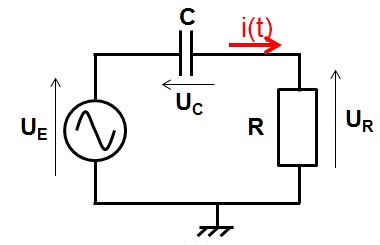
\includegraphics[scale=0.5]{images/circuit_RC_reponse_forcee.jpg}
	\end{minipage}
	\vspace{0.5\baselineskip}

	La réponse du circuit $U_{R}$ est la superposition de la
        réponse naturelle $U_{R0}$ et de la réponse forcée
        $U_{Rf}$. La réponse naturelle est liée à la présence d'une
        condition initiale : ici, le stockage d'une charge dans le
        condensateur à t=0. Sans charge initialement stockée, la
        réponse naturelle aurait été nulle. Nous avions établi la
        réponse naturelle de ce circuit en terme de courant. Nous
        pouvons aisément l'adapter pour la donner en terme de tension
        de sortie.
	\begin{equation*}\label{}
          U_{R0}(t)=Ri_{0}(t)=U_{C0}\expo{-\frac{t}{RC}}~,~~t>0
	\end{equation*}

        La réponse forcée est provoquée par l'excitation du circuit en
        t > 0, indépendamment de la présence d'une condition
        initiale. Commençons par établir une équation différentielle
        reliant la tension de sortie $U_{Rf}$ et l'excitation
        $U_{E}(t)$. On utilise la loi des mailles. Après une
        dérivation, on obtient l'équation
        \ref{equa_diff_reponse_forcee_RC}.
	\begin{equation*}\label{}
          U_{E}(t)=U_{C}(t)+U_{R}(t) ~ \Rightarrow ~ U_{E}(t)=\frac{1}{C}\int i(t) \deriv t+U_{R}(t)~ \Rightarrow ~U_{E}(t)=\frac{1}{RC}\int U_{R}(t) \deriv t+U_{R}(t)
	\end{equation*} 
	\begin{equation}\label{equa_diff_reponse_forcee_RC}
          \frac{dU_{E}}{dt}=\frac{U_{R}}{RC}+\frac{dU_{R}}{dt}
	\end{equation}

	L'excitation étant de type exponentielle complexe et le
        circuit linéaire, la réponse est aussi de type exponentielle
        complexe. Elle s'écrit : $U_{Rf}(t)=Y\expo{pt}$. Replaçons les
        termes $U_{E}$ et $U_{R}$ par leurs expressions respectives
        dans \ref{equa_diff_reponse_forcee_RC} et exprimons le rapport
        entre ces deux grandeurs pour obtenir la fonction de transfert
        H(p) de ce circuit (équation \ref{TF_RC_forcee}).
	\begin{equation*}
          pX\expo{pt}=\frac{1}{RC} Y\expo{pt}+pY\expo{pt} ~\Rightarrow~pU_{E}(t)=\frac{1}{RC}U_{Rf}(t)+pU_{Rf}(t)
	\end{equation*}
	\begin{equation}\label{TF_RC_forcee}
          H(p)=\frac{U_{Rf}}{U_{E}}(p)=\frac{p}{p+\frac{1}{RC}}=\frac{p}{p+\omega_{0}}~,~\omega_{0}=\frac{1}{RC}
	\end{equation}

	La fonction de transfert du système présente un zéro nul et un
        seul pôle $p_{0}$, qui est exactement le même que celui
        identifié dans l'analyse de la réponse naturelle. Ce n'est pas
        une surprise car les pôles agissent sur la stabilité, qui est
        une caractéristique intrinsèque du système indépendante de
        l'excitation. Le pôle étant purement réel et négatif, on peut
        conclure que le système sera stable.
		
	Calculons maintenant la réponse forcée à un signal
        cosinusoïdale, en utilisant
        \ref{calcul_reponse_fonction_transfert}. Le système n'agit que
        sur l'amplitude et la phase de l'excitation. Il est donc
        intéressant d'exprimer la fonction de transfert sous la forme
        de son module et son déphasage. En considérant $p=j\omega$,
        celles-ci sont :
	\begin{equation*}
          |H(\omega)|=\frac{\omega}{\sqrt{\omega^{2}+\omega_{0}^{2}}}~~~et~~Arg(H(\omega))=\frac{\pi}{2}-atan(\frac{\omega}{\omega_{0}})
	\end{equation*}
	\begin{equation*}
          \Rightarrow~U_{Rf}(t)=|H(\omega)|cos(\omega t+Arg(H(\omega)))
	\end{equation*}
	La réponse étant la superposition des réponses naturelles et
        forcées, celle-ci s'écrit :
	\begin{equation*}
          \Rightarrow~U_{R}(t)=U_{Rf}(t)+U_{R0}(t)=|H(\omega)|cos(\omega t+Arg(H(\omega)))+U_{C0}\expo{-\frac{t}{RC}}
	\end{equation*}
	
	\vspace{1\baselineskip}

	\subsection{Calcul de la réponse d'un système dans le domaine
          temporel ou fréquentiel ?}
	
	Nous venons de décrire deux manières de calculer l'effet d'un
        système LTI, selon que l'on considère une excitation
        impulsionnelle ou exponentielle complexe. Dans le premier cas,
        la réponse est déterminée directement dans le domaine temporel
        à l'aide de l'équation \ref{Demo_produit_convolution} et de la
        réponse impulsionnelle, à l'aide d'un produit de
        convolution. Dans le second cas, la réponse est déterminée
        dans le domaine fréquentiel à l'aide de l'équation
        \ref{calcul_reponse_fonction_transfert} et de la fonction de
        transfert.  Bien qu'il semble plus naturel de faire le calcul
        de la réponse directement dans le domaine temporel, nous avons
        montré que le calcul dans le domaine fréquentiel était
        beaucoup plus évident. Il se résume à une simple
        multiplication de l'excitation par la fonction de transfert.
        Cependant, comme il s'agit du même système, il y a
        nécessairement un lien entre la réponse impulsionnelle et la
        fonction de transfert. C'est ce que nous verrons dans les
        prochains chapitres, où nous aborderons les questions de
        transformée de Laplace, puis de Fourier. Nous allons ainsi
        mettre en évidence des transformations mathématiques,
        permettant le passage d'une fonction du domaine temporel au
        domaine fréquentiel, et inversement.
	
	\vspace{1\baselineskip}

	
	
	\section{Exercices}
	
	\subsubsection{Exercice 1} 
	Soient les systèmes dont le comportement temporel est défini
        par les équations suivantes. Indiquez si ces systèmes sont
        linéaires, à temps invariant et causaux ?
	
	a. $y(t) = x(t)+4\frac{dy}{dt}$
	
	b. $y(t) = 2x(t)+2$
	
	c. $y(t)=\expo{-t}x(t-2)^{2}$
	
	d. $y(t)=\frac{dx}{dt}+x(t+2)$
	
	\vspace{1\baselineskip}
	
	\subsubsection{Exercice 2} 
	1. On trace les réponses de deux systèmes LTI ((a) et
        (b)). Proposez une expression mathématique décrivant ces
        réponses.
	\begin{figure}[htbp]
          \centering 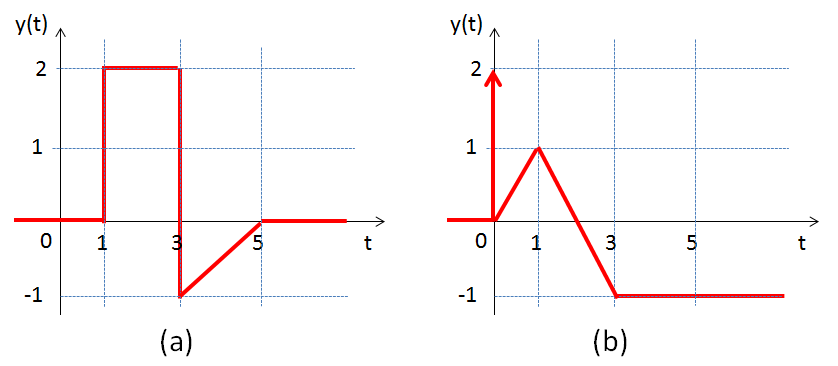
\includegraphics[scale=0.5]{images/Exo_2_2.jpg}
	\end{figure}

	
	2. Réécrivez sous la forme d'une fonction à valeurs réelles
        les fonctions suivantes et esquissez leur forme temporelle
        (pour t >0) :
	
	a. $x(t) = (1+j)\expo{j 10t}$
	
	b. $y(t) = \expo{(-2+j)t} u(t-2)$
	
	c. $z(t) = \expo{(-1+2j)t}+\expo{(-1-2j)t}$
	
	\vspace{1\baselineskip}
	
	
	
	\subsubsection{Exercice 3}
	
	On dispose de la réponse indicielle d'un système linéaire, qui est esquissée ci-dessous. Elle a une forme exponentielle croissante.\\
	
	\begin{figure}[htbp]
          \centering 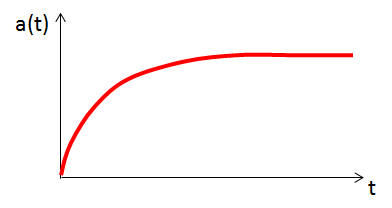
\includegraphics[scale=0.5]{images/Exo_2_3.png}
	\end{figure}
	
	Esquissez les réponses de ce système dans les cas suivants :\\
	
	a. l'excitation $e(t)=u(t)-u(t-1)$\\
	
	b. l'excitation $e(t)=t(u(t)-u(t-2))$\\
	
	c. l'excitation est la dérivée de celle utilisée pour obtenir la réponse indicielle.\\
	
	\subsubsection{Exercice 4}
	
	On excite un système linéaire à l'aide du signal suivant : $e(t)=\expo{j2\pi t}$. La réponse obtenue, notée y(t), est égale à $y(t)=\frac{1}{2}\expo{j(2\pi t+\frac{\pi}{3})}$.\\
	
	a. Réécrire la réponse sous la forme $y(t)=Acos(\omega t + \phi)$ et $y(t)=Bcos(\omega t)+Csin(\omega t)$, en précisant les valeurs de A, B, C et $\phi$.\\
	
	b. Donnez l'expression de la réponse du système lorsqu'il est
        excité par le signal ci-dessous.
	
	\begin{figure}[htbp]
          \centering 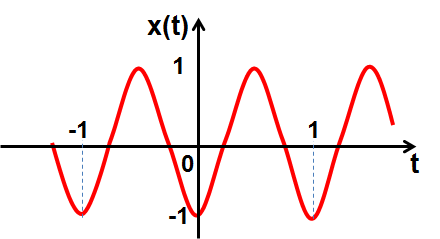
\includegraphics[scale=0.5]{images/Exo_2_4.png}
	\end{figure}
	
	c. Calculez la réponse du système à l'excitation suivante : $x(t)=\frac{3\sqrt{3}}{2}cos(2\pi t)+\frac{1}{2}sin(2\pi t)$.\\
	
	
	
	\subsubsection{Exercice 5 - Réponse indicielle d'un circuit
          RC}
	
	On reprend le circuit RC dont on a étudié la réponse dans la
        partie VI.3. On considère deux cas : celui où le condensateur
        est déchargé initialement, puis celui où il est chargé.
	
	a. Calculez la réponse naturelle du circuit lorsque le
        condensateur est initialement chargé.
	
	b. En déduire la réponse impulsionnelle du circuit.
	
	c. Calculez la réponse lorsque le circuit est soumis à un
        échelon de \Heaviside{} d'amplitude E, dans les deux cas (charge
        initiale absente ou présente).
	
	d. En déduire la réponse indicielle du circuit.
	
	\vspace{1\baselineskip}
	

	
	\subsubsection{Exercice 6}
	
	On considère les deux circuits électriques ci-dessous. Pour le
        circuit (a), la tension initiale (t=0) aux bornes du
        condensateur C est notée $U_{C0}$. Pour le circuit (b), un
        courant noté $I_L0$ traverse la bobine L. La sortie de ces
        deux circuits est la tension $U_{S}$.
	
	\begin{figure}[htbp]
          \centering 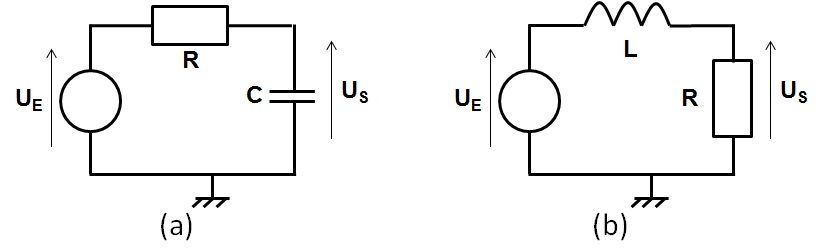
\includegraphics[scale=0.5]{images/Exo_2_4.jpg}
	\end{figure}
	
	a. Déterminez les fréquences et les réponses naturelles de ces
        deux circuits. Quels sont les ordres de ces deux systèmes ?
	
	b. On excite ces deux systèmes à l'aide d'un échelon de
        \Heaviside{} d'amplitude notée E. Déterminez la réponse
        indicielle de ces deux circuits.
	
	c. Déterminez les fonctions de transfert de ces deux circuits.
	
	\vspace{1\baselineskip}
	
	\subsubsection{Exercice 7 - Fonction de transfert d'un circuit
          résonant}
	
	On reprend le circuit RLC présenté dans la partie
        IV.4. Celui-ci est excité par un générateur de courant I,
        comme le montre la figure ci-dessous. On s'intéresse à la
        tension U aux bornes de ce circuit. On considère que la
        résistance R est grande et $R>>\sqrt{\frac{L}{C}}$.
 	 	
 	\begin{figure}[htbp]
          \centering 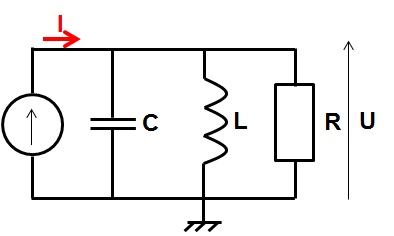
\includegraphics[scale=0.5]{images/Exo_2_5.jpg}
 	\end{figure}
 
 	a. Déterminez la fonction de transfert de ce circuit. La mettre sous la forme $\frac{Gp}{p^2+2\alpha p+\omega_{0}^{2}}$.\\
 	
 	b. Précisez l'unité de la fonction de transfert. \\
 	
 	c. Ce circuit est-il stable ?\\
 	
 	d. On considère maintenant que le terme $\alpha$ est négligeable et une excitation cosinusoïdale du circuit. Y a t-il une fréquence particulière où la réponse présente un maximum ? Si oui, laquelle ? \\
 	
 	e. Donnez l'expression de la réponse temporelle du circuit en régime permanent.\\
	
	\vspace{1\baselineskip}
	
	\subsubsection{Exercice 8}
	
	On considère le système dont le fonctionnement est décrit par
        le schéma-bloc ci-dessous. Celui-ci transforme un signal
        d'entrée e(t) et délivre en sortie un signal s(t).
	
	\begin{figure}[htbp]
          \centering 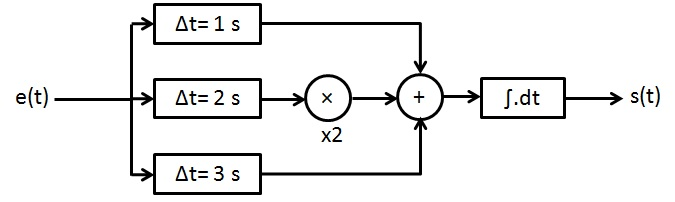
\includegraphics[scale=0.5]{images/Exo_2_6.jpg}
	\end{figure}
	
	a. Le système est-il linéaire, à temps invariant, causal ?
	
	b. Ecrire l'équation différentielle générale de ce système.
	
	c. Déterminez l'expression de la réponse impulsionnelle h(t)
        du système. Esquissez l'allure temporelle de la réponse
        impulsionnelle.
	
	d. Déterminez l'expression de la fonction de transfert H(p) du
        système. Précisez les pôles de la fonction de transfert. Que
        concluez-vous sur sa stabilité ?
	

	



        %%% Pour compiler avec emacs Local Variables: mode: latex
        %%% TeX-master: "main" End:

\cleardoublepage
\chapterimage{poly/Pictures/portrait_charge_bouilly_laplace.png} % Table of contents heading image
\chapter{Transformée de Laplace}	
\label{chap:laplace}	
	Dans le chapitre précédent, nous avons identifié deux manières de calculer la réponse transitoire d'un système :
	\begin{itemize}
		\item soit en considérant la réponse impulsionnelle et en calculant le produit de convolution dans le domaine temporel
		\item soit en considérant la fonction de transfert et en réalisant une simple multiplication dans le domaine fréquentiel, nécessitant une excitation exponentielle complexe.\\
	\end{itemize}

	Bien que cette deuxième méthode soit plus simple, elle suppose une excitation d'un type donné. La question posée et illustrée ci-dessous est : peut-on passer directement d'une fonction temporelle à sa forme dans le domaine fréquentiel complexe, même si celle-ci n'est pas une exponentielle complexe ? Nous allons voir que cela est possible, via une transformation mathématique appelée transformée de Laplace. En plus de nous offrir un moyen pratique pour déterminer les réponses des systèmes quel que soit le type d'excitation, nous verrons  qu'elle permet de résoudre d'une manière pratique les équations différentielles ordinaires, quel que soit leur ordre (on pourra remarquer qu'il s'agit en fait du même problème). 
	
	\begin{figure}[h!]
		\centering
		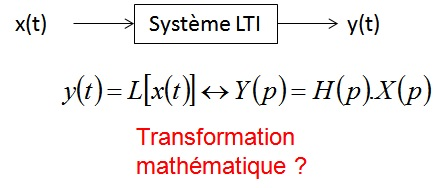
\includegraphics[scale=0.5]{images/Position_Pb_Laplace.jpg}
		\caption{Lien entre la réponse impulsionnelle et la fonction de transfert}	
		\label{Fig:Position_Pb_Laplace} 
	\end{figure}
	
	 La transformée de Laplace permet de passer du domaine temporel à son domaine dual, le domaine fréquentiel. Dans les chapitres suivants, nous présenterons un autre type de transformation dérivée de la transformée de Laplace : la transformée de Fourier, qui sera très utile pour l'analyse des signaux, ainsi que pour l'étude des systèmes en régime permanent.
	
	\vspace{0.5\baselineskip}
	\underline{Remarque :}
	Dans ce chapitre, on ne considère que des fonctions causales. L'instant d'apparition des signaux se fera en t = 0. Pour représenter cette condition, l'ensemble des signaux en entrée et en sortie que nous allons considérer seront multiplier par l'échelon de Heaviside u(t).
	\vspace{1\baselineskip}
	
	\section{Transformation d'une fonction temporelle au domaine fréquentiel}
	Dans le domaine temporel, l'entrée et la sortie du système sont reliées par la réponse impulsionnelle h(t) et le produit de convolution. Cela est vrai quel que soit le type d'excitation appliquée en entrée du système. Le passage dans le domaine fréquentiel suppose une excitation exponentielle complexe. Considérons ce cas dans le domaine temporel : la réponse sera donc égale au produit de convolution entre la réponse impulsionnelle et l'excitation exponentielle complexe. Nous considérons dans un premier temps un signal défini sur tout le domaine temporel. Elle peut être modifiée selon la forme donnée par l'équation \ref{Demo_Laplace}.
	
	\begin{equation}\label{}
	y(t) = h*x(t) = h * exp(pt) = \int_{-\infty}^{+\infty} h(\tau) \cdot exp(p(t-\tau))
 \deriv \tau 	
 	\end{equation}
	\begin{equation}\label{Demo_Laplace}
	y(t) = exp(pt) \int_{-\infty}^{+\infty} h(\tau) \cdot exp(-p\tau)
	\deriv \tau 	
	\end{equation}
	
	On remarque que la réponse du système est le produit entre l'excitation et un terme intégrale dépendant de la réponse impulsionnelle. On retrouve donc une forme très similaire à celle vue à l'équation \ref{Def_fonction_tranfert}, reliant réponse et excitation exponentielle complexe, via la fonction de transfert. Ce terme intégrale n'est donc rien d'autre que la réponse du système LTI dans le domaine fréquentiel complexe, c'est-à-dire sa fonction de transfert.
	\begin{figure}[h!]
		\centering
		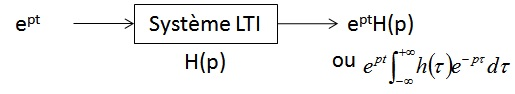
\includegraphics[scale=0.7]{images/LTI_Laplace.jpg}
		\caption{Lien via la transformée de Laplace entre l'excitation exponentielle complexe et la réponse d'un système LTI}	
		\label{Fig:LTI_Laplace} 
	\end{figure}
	
	Nous venons de mettre en évidence une transformation mathématique permettant de passer de la représentation temporelle d'une fonction à sa représentation fréquentielle complexe. Cette transformée s'appelle la transformée de Laplace. Elle est donnée par \ref{Fonction_Transfert_Laplace_non_causale} dans le cas général.
	\begin{equation}\label{Fonction_Transfert_Laplace_non_causale}
	H(p) = \int_{-\infty}^{+\infty} h(t) \cdot exp(-pt)	\deriv t~,~~p \in \mathbb{C}	
	\end{equation}	
	
	La démonstration précédente reste valable dans le cas d'un signal causal, défini pour t > 0. Dans ce cas, on peut écrire :
	\begin{equation}\label{Fonction_Transfert_Laplace_causale}
	H(p) = \int_{0}^{+\infty} h(t) \cdot exp(-pt)	\deriv t~,~~p \in \mathbb{C}	
	\end{equation}
	
	\textbf{\underline{Remarque :}}
	On vient aussi de montrer que la fonction de transfert, exprimée dans le domaine des fréquences complexes p, n'est rien d'autre que la transformée de Laplace de la réponse impulsionnelle.\\
	
	\section{Transformée de Laplace}
	\subsection{Définition}
	La transformée de Laplace est une transformation mathématique, transformant une fonction temporelle en une fonction définie dans le domaine des fréquences complexes p. Nous noterons $\mathcal{L}$ cette transformation. On distingue deux types de transformée de Laplace : bilatérale (\ref{Transfo_Laplace_non_causale}) et unilatérale (\ref{Transfo_Laplace_causale}). Cette dernière s'impose naturellement dès que l'on considère des systèmes causaux (h(t) = 0 pour t <0). Dans la suite, comme nous ne traiterons que de systèmes causaux, nous ne considérerons que la transformée de Laplace unilatérale.
	\begin{equation}\label{Transfo_Laplace_non_causale}
	F(p) = \mathcal{L}[f(t)] = \int_{-\infty}^{+\infty} f(t) \cdot exp(-pt)	\deriv t~,~~p=\sigma + j \omega	
	\end{equation}
	\begin{equation}\label{Transfo_Laplace_causale}
	F(p) = \mathcal{L}[f(t)] = \int_{0^{+}}^{+\infty} f(t) \cdot exp(-pt)	\deriv t~,~~p=\sigma + j \omega	
	\end{equation}
	
	\underline{\textbf{Opérateur de Heaviside s :}}\\
	Dans la littérature scientifique anglo-saxonne, lorsque la transformée de Laplace est utilisée, l'opérateur p, représentant les fréquences complexes, apparait rarement. Il est remplacé par un opérateur noté "s" et appelé opérateur de Heaviside en hommage à Oliver Heaviside. Il est l'inventeur des méthodes mathématiques de résolution des équations différentielles pour les circuits électroniques, équivalentes à la transformée de Laplace.\\
	
	

	
	\subsection{Conditions d'existence de la transformée de Laplace et stabilité des systèmes}
	Il est important de noter que la transformée de Laplace n'existe que si l'intégrale converge. Ceci n'est pas le cas pour toutes les valeurs de p.
	L'objectif de ce cours n'est pas de faire ce calcul intégrale, mais plutôt de l'utiliser comme outil pour l'étude des systèmes linéaires. Nous utiliserons la plupart du temps des tables contenant les transformées pour les fonctions les plus courantes. Néanmoins, nous allons mettre en œuvre ce calcul à travers un exemple et indiquer les conditions d'existence de la transformée de Laplace. Nous allons mettre en évidence ce que cela signifie du point de vue de la stabilité des systèmes LTI. Par souci de simplification, on dira qu'un système est stable s'il converge vers une valeur finie.
	Exemple : considérons un système LTI dont la réponse impulsionnelle est définie par la fonction : $h(t) = exp(\alpha t)u(t) $ où $\alpha$ est un réel quelconque.
	Calculons sa transformée de Laplace à l'aide de l'équation \ref{Transfo_Laplace_non_causale} :
	\begin{equation*}
	H(p) = \mathcal{L}[exp(\alpha t)u(t)] = \int_{-\infty}^{+\infty}exp(\alpha t)u(t) \cdot exp(-pt) \deriv t
	\end{equation*}
	\begin{equation*}
	H(p) = \int_{0}^{+\infty}exp(-(p-\alpha) t) \deriv t
	\end{equation*}
	\begin{equation*}
	H(p) = \lim_{T \to +\infty} \frac{1-exp(-(p-\alpha)T)}{p-\alpha} = \lim_{T \to +\infty} \frac{1-exp(-(\sigma-\alpha)T)exp(-j\omega T)}{p-\alpha}
	\end{equation*}
	La transformée de Laplace existera si cette intégrale converge. Cela dépend uniquement de la partie réelle $\sigma$ de la fréquence complexe :
	\begin{equation}\label{}
	F(p) = \left \{
	\begin{array}{l l}
	\frac{1}{p-\alpha}  & si~\sigma>\alpha \\
	\infty   & sinon \\
	\end{array}
	\right .	 	
	\end{equation}
	
	Si on représente l'excitation en fréquence dans le plan P, il existe un
	domaine d'existence de la transformée de Laplace appelé domaine de
	convergence. Il s'agit d'un plan où Re(p) = $\sigma $ \textgreater{} $\alpha $. Nous le
	représentons dans deux cas différents :  $\alpha $ \textless{} 0 et  $\alpha $
	\textgreater{} 0, et allons analyser sa signification concrète.
	\begin{figure}[h!]
		\centering
		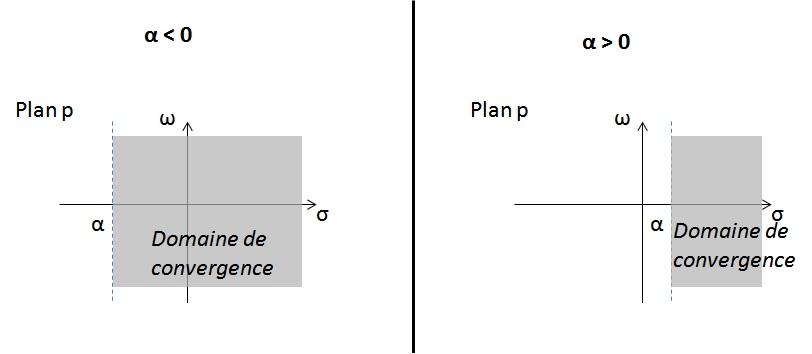
\includegraphics[scale=0.8]{images/Domaine_convergence_exp_at.jpg}
		\caption{Domaine de convergence de la fonction $exp(\alpha t)$}	
		\label{Fig:Domaine_convergence_exp_at} 
	\end{figure}
	Le domaine de convergence indique, dans le cas d'une excitation
	exponentielle complexe, l'ensemble des fréquences complexes pour lequel
	le système convergera. Pour s'en
	convaincre, considérons une excitation exponentielle, de fréquence
	complexe $p_{0} =  \beta +j \omega $. Reprenons la forme initiale dérivée de la réponse	impulsionnelle.
	\begin{equation*}
	y(t) = exp(p_{0}t)\int_{-\infty}^{+\infty}h(\tau)exp(-p_{0}\tau) \deriv \tau 
	\end{equation*}
	\begin{equation*}
	y(t) = exp((\beta+j\omega)t)\int_{-\infty}^{+\infty}exp(\alpha \tau)exp(-(\beta+j\omega)\tau) \deriv \tau 
	\end{equation*}
	\begin{equation*}
	y(t) = exp((\beta+j\omega)t)\int_{-\infty}^{+\infty}exp(-(\beta-\alpha+j\omega)\tau) \deriv \tau 
	\end{equation*}
	\begin{equation}
	y(t) = \lim_{T \to +\infty} \frac{exp((\beta+j\omega)t)(exp(-(\beta-\alpha+j\omega)T)-1)}{\beta-\alpha+j\omega} 
	\end{equation}
	Cette fonction converge si la partie réelle $\beta $ de la fréquence de
	l'excitation est supérieure à  $\alpha $, autrement dit si la fréquence complexe
	d'excitation appartient au domaine de convergence, mais aussi si $\beta $
	\textless{} 0. Dans le cas contraire, le signal d'entrée va diverger pour
	t \textgreater{} 0. Cette double condition sur $\beta $ n'est possible que si $\alpha $
	\textless{} 0, qui est donc une condition nécessaire pour garantir la stabilité du système.\\
	
	\textbf{\underline{Cas d'une excitation harmonique :}}
	
	Cette situation correspond au cas où $\beta $ = 0. Le système sera stable
	uniquement si, dans le plan p, l'axe des imaginaires appartient au
	domaine de convergence. Dans le chapitre consacré à la transformée de
	Fourier, nous verrons qu'elle est équivalente à une transformée de
	Laplace, mais pour une fréquence purement complexe $\beta $ = 0. Si l'axe des
	imaginaires appartient au domaine de convergence, alors la transformée
	de Fourier de la fonction pourra exister.\\
	
	\subsection{Pôles et zéros d'une fonction de transfert}
	
	Reprenons l'exemple précédent. Comme nous l'avions introduit dans le
	chapitre précédent, $\alpha $ correspond à un pôle de la réponse du système. Sa
	stabilité est liée à sa partie réelle.~
	
	Toutes les transformées de Laplace que l'on considère peuvent se mettre sous la forme d'une fonction rationnelle, où le numérateur N(p) et dénominateur D(p) sont
	des polynômes. Eux-mêmes peuvent être exprimés en fonction de leurs
	racines appelés zéros et pôles respectivement. Ceux-ci correspondent à
	des fréquences complexes particulières qui :
	\begin{itemize}
		\item annulent la fonction de transfert dans le cas des zéros p\textsubscript{zi}
	
		\item font tendre la fonction de transfert vers l'infini dans le cas des pôles p\textsubscript{pj}
	\end{itemize}
	
	\begin{equation}\label{key}
	F(p) = \frac{N(p)}{D(p)} = \frac{b_{m}p^{m}+...+b_{1}p+b_{0}}{a_{n}p^{n}+...+a_{1}p+a_{0}} ~\Rightarrow ~ F(p) = G \frac{\prod_{i=1}^{m}(p-p_{zi})}{\prod_{i=1}^{n}(p-p_{pj})}
	\end{equation}
	où G est le gain de la fonction de transfert.
	Comme nous l'avions déjà vu dans le chapitre 2, la position des pôles nous donne une indication sur l'allure temporelle de la fonction de transfert (réponse naturelle).
	Quel que soit le système linéaire considéré, la position de ces pôles va déterminer la stabilité du système. Vous approfondirez ces concepts dans le cours d'automatique.
	
	\section{Propriétés de la transformée de Laplace}
	Dans cette partie, nous allons passer en revue plusieurs des propriétés importantes de la transformée de Laplace, qui facilitent les calculs de la transformée de Laplace et les applications associées. Nous ne démontrerons pas l'ensemble de ces propriétés.
	\subsection{Linéarité}
	La transformée de Laplace est linéaire. La transformée de Laplace d'une somme pondérée de fonction est la somme des transformées de Laplace individuelle de ces fonctions, pondérées de la même manière. Elle vérifie donc la relation suivante :
	\begin{equation}\label{key}
	a \cdot f(t)+b \cdot g(t) \longleftrightarrow a \cdot F(p)+b \cdot G(p)~~,~avec~F(p)=\mathcal{L}[f(t)]~et~G(p)=\mathcal{L}[g(t)]
	\end{equation}
	
	\subsection{Théorème du retard}
	
	Supposons que l'on connaisse la transformée de Laplace F(p) de la
	fonction causale f(t), qui est nulle pour t \textless{} 0. Si on a
	retardé de t\textsubscript{0} cette fonction, elle devient
	f(t-t\textsubscript{0}) et s'annule pour tout t \textless{}
	t\textsubscript{0}. Calculons sa transformée de Laplace à partir de (\ref{Transfo_Laplace_causale})
	et appliquons le changement de variable w = t-t\textsubscript{0}. On
	montre que la transformée de Laplace de la fonction retardée est la
	transformée de Laplace non retardée multipliée par $e^{-pt_{0}}$.
	
	\begin{equation*}
	F_{t0}(p) = \mathcal{L}[f(t-t_{0})]=\int_{t_{0}}^{+\infty}f(t-t_{0})exp(-pt) \deriv t   
	\end{equation*}
	\begin{equation*}
	F_{t0}(p) = \int_{0}^{+\infty}f(w)exp(-p(w+t_{0})) \deriv w = \int_{0}^{+\infty}f(w)exp(-pw)exp(-pt_{0}) \deriv w  
	\end{equation*}
	\begin{equation}\label{}
	F_{t0}(p) = F(p)\cdot exp(-pt_{0})
	\end{equation}
	
	\subsection{Théorème du changement d'échelle}
	
	Supposons que l'on connaisse la transformée de Laplace F(p) de la
	fonction causale f(t). Dilatons l'échelle de temps de cette fonction par
	un facteur réel k. La fonction devient f(kt). Calculons la transformée
	de Laplace de cette version dilatée de f(t), en appliquant le changement
	de variable $w = kt$.
	\begin{equation*}
	F_{k}(p) = \mathcal{L}[f(kt)]=\int_{t_{0}}^{+\infty}f(kt)exp(-pt) \deriv t  =\int_{t_{0}}^{+\infty}\frac{1}{k}f(w)exp(-\frac{p}{k}w) \deriv w 
	\end{equation*}
	\begin{equation}\label{}
	F_{k}(p) = \frac{1}{k}\cdot F(\frac{p}{k})
	\end{equation}
	
	
	\subsection{Translation dans le domaine fréquentiel}
	Un décalage d'une valeur $p_{1}$ dans le domaine de Laplace conduit à une multiplication par $e^{p_{1}t}$ dans le domaine temporel.
	\begin{equation}\label{key}
		soit~F(p)=\mathcal{L}[f(t)]~alors~\mathcal{L}[e^{p_{1}t}f(t)] = F(p-p_{1})	
	\end{equation}
	
	Dans le domaine fréquentiel ($\alpha$ = 0), cela est équivalent à une translation du spectre. Ce procédé est bien connu en télécommunication, car il est utilisé pour moduler les signaux à transmettre.
	
	
	
	\subsection{Dérivation dans le domaine temporel}
	Considérons le cas d'une fonction f(t) continue non nulle pour t > 0. La transformée de Laplace de la dérivée de cette fonction est donnée par :
	
	\begin{equation}\label{key}
	\mathcal{L}[\frac{df}{dt}] = p\cdot F(p)-f(0^{+}) ~~~avec~f(0^{+})=\lim_{t\rightarrow0^{+}}f(t)
	\end{equation}

	On remarque que l'opérateur dérivée correspond à une multiplication de
	la transformée de Laplace par p. Cependant, il est nécessaire de tenir
	compte de la condition initiale f(0\textsuperscript{+}).
	
	Il est possible de généraliser cette relation au cas où l'on dérive N
	fois la fonction. L'expression devient :
	\begin{equation}\label{key}
	\mathcal{L}[\frac{d^{n}f}{dt^{n}}] = p^{n}\cdot F(p)-p^{n-1}\cdot f(0^{+})-p^{n-2}\cdot \frac{df}{dt}(0^{+})-...-p\frac{d^{n-2}f}{dt^{n-2}}(0^{+})-\frac{d^{n-1}f}{dt^{n-1}}(0^{+})
	\end{equation}
	Le calcul nécessite de connaître les conditions initiales non seulement sur la valeur de la fonction mais aussi pour ses (n-1) premières dérivées.
	
	\subsection{Dérivation dans le domaine des fréquences complexes p}
	Dériver une fonction dans le domaine de Laplace revient à multiplier cette fonction par -t dans le domaine temporel.
	\begin{equation}\label{key}
		soit~F(p)=\mathcal{L}[f(t)]~alors~\mathcal{L}[-t\cdot f(t)] = \frac{dF(p)}{dp})
	\end{equation}
	
	Cette propriété peut se généraliser au cas où l'on dérive N fois la fonction dans le domaine de Laplace, qui revient à multiplier la fonction temporelle par le terme $(-t)^{N}$.
	\begin{equation}\label{key}
	soit~F(p)=\mathcal{L}[f(t)]~alors~\mathcal{L}[-(t)^{n}\cdot f(t)] = \frac{dF^{n}(p)}{dp^{n}})
	\end{equation}
	
	
	\subsection{Intégration temporelle}
	Considérons le cas d'une fonction f(t) continue non nulle pour t > 0. La transformée de Laplace de son intégrale de 0 à t est donnée par :
	\begin{equation}\label{key}
		soit~F(p)=\mathcal{L}[f(t)]~alors~\mathcal{L}[\int_{0}^{t}f(\tau)d\tau]=\frac{F(p)}{p}	
	\end{equation}
	
	Cette propriété peut s'étendre au cas où on intègre N fois la fonction temporelle :
	
	\begin{equation}\label{key}
	soit~F(p)=\mathcal{L}[f(t)]~alors~\mathcal{L}[\int ... \int_{0}^{t}f(\tau)d\tau]=\frac{F(p)}{p^{n}}	
	\end{equation}
	

	\subsection{Théorème de la valeur initiale}
	
	On considère une fonction f(t) continue non nulle pour t > 0. On peut montrer que :
	\begin{equation}\label{key}
		\lim_{t \to 0^{+}}f(t) = \lim_{p \to +\infty}pF(p)
	\end{equation}
	
	
	\subsection{Théorème de la valeur finale}
	De la même manière, on peut montrer que la fonction f(t) tend de manière asymptotique vers la valeur suivante :
	\begin{equation}\label{key}
		\lim_{t \to +\infty}f(t) = \lim_{p \to 0}pF(p)
	\end{equation}
	
	Cette propriété, couplée à celle de l'intégration temporelle, permet aussi de calculer l'aire sous la courbe temporelle entre 0 et une valeur t > 0 :
	\begin{equation}\label{key}
		\int_{0^{-}}^{t}f(t)dt=F(0)
	\end{equation}
	
	\subsection{Multiplication et produit de convolution}
	Multiplication et produit de convolution (\ref{Demo_produit_convolution}) sont deux opérations complémentaires dans les domaines temporelles et de Laplace. On peut ainsi écrire les deux propriétés suivantes :
	\begin{equation}\label{key}
		\mathcal{L}[f(t)\cdot g(t)] = F*G(p)
	\end{equation}
	\begin{equation}\label{key}
	\mathcal{L}[f*g(t)] = F(p) \cdot G(p)
	\end{equation}
	
	Avec cette dernière propriété, on retrouve la relation vue entre la fonction de transfert et la réponse impulsionnelle. Dans le domaine temporel, la réponse d'un système correspond au produit de convolution entre l'excitation et la réponse impulsionnelle. Avec une excitation exponentielle complexe, cette relation est équivalente au produit entre l'excitation exprimée dans le domaine de Laplace et la fonction de transfert, soit la transformée de Laplace de la réponse impulsionnelle.
	
	\subsection{Fonctions causales avec N répétitions}
	On considère une fonction $f_{1}(t)$, dite génératrice, que l'on répète N fois de manière périodique pour former une nouvelle fonction causale f(t). La période est notée T. La fonction f(t) s'écrit :
	\begin{equation*}
	f(t)=\sum_{k=0}^{N-1}f_{1}(t-kT)
	\end{equation*}
	
	On note $F_{1}(p)$ la transformée de Laplace de la fonction génératrice. A partir du théorème du retard, on peut calculer la transformée de Laplace de la somme des N termes précédents.
	\begin{equation*}
	F(p)=\mathcal{L}[f(t)]=F_{1}(p)(1+e^{-Tp}+e^{-2Tp}+...+e^{-(N-1)Tp})
	\end{equation*}
	On retrouve une série de N termes exponentiels mis à la puissance k, qui peut se simplifier selon la relation ci-dessous. 
	\begin{equation}
	F(p)=\mathcal{L}[f(t)]=F_{1}(p)\frac{1-e^{-(N-1)Tp}}{1-e^{-Tp}}
	\end{equation}
	
	
	\subsection{Fonctions périodiques causales}
	La propriété précédente peut être réutilisée pour déterminer la transformée de Laplace d'une fonction causale périodique, de période T et générée à partir d'une fonction génératrice $f_{1}(t)$. La fonction périodique s'écrit : $f(t)=\sum_{k=0}^{+\infty}f_{1}(t-kT)$.
	
	On en déduit la transformée de Laplace de la fonction en remarquant que $|e^{-kTp}| < 1$ car la partie réelle de p est positive pour garantir la convergence.
	\begin{equation}
	F(p)=\mathcal{L}[f(t)]=\lim_{N \to +\infty}F_{1}(p)\frac{1-e^{-(N-1)Tp}}{1-e^{-Tp}}=F_{1}(p)\frac{1}{1-e^{-Tp}}
	\end{equation}
	
	Toute fonction exprimée dans le domaine de Laplace où apparaît le terme $\frac{1}{1-e^{-Tp}}$ correspond à la transformée de Laplace d'une fonction périodique de période T.
	
	\vspace{1\baselineskip}
		
	
	\section{Transformée de Laplace des fonctions courantes}
	Le tableau \ref{Tab:Transfo_Laplace_usuelle} donne la transformée de Laplace des fonctions causales les plus courantes, et pour lesquelles des formes mathématiques simples existent. Pour la plupart, aucune démonstration n'est donnée, mais les transformées peuvent être retrouvées. Nous nous limiterons à deux exemples de mise en forme de la transformée de Laplace pour deux formes temporelles courantes, sachant que nous avons déjà vu celle d'une fonction exponentielle.\\
	
	\underline{Exemple 1 :} échelon unitaire f(t) = u(t)
	\begin{equation*}
	F(p)=\mathcal{L}[u(t)] = \int_{-\infty}^{+\infty}u(t)exp(-pt) \deriv t =\int_{0}^{+\infty}exp(-pt) \deriv t = [-\frac{exp(pt)}{p}]_{0}^{+\infty}=\frac{1}{p}
	\end{equation*}
	
	\underline{Exemple 2 :} fonction cosinusoïdale
	\begin{equation*}
	f(t)=cos(\omega t)u(t)
	\end{equation*}
	\begin{equation*}
	F(p)=\mathcal{L}[f(t)]=\int_{-\infty}^{+\infty}cos(\omega t)u(t) \deriv t=\int_{0}^{+\infty}\frac{exp(j\omega t)+exp(-j\omega t)}{2} \deriv t
	\end{equation*}
	\begin{equation*}
	F(p)=\frac{1}{2}\int_{0}^{+\infty}(exp((j\omega-p) t)+exp(-(j\omega+p) t)) \deriv t=\frac{1}{2}([\frac{exp((j\omega-p) t)}{j\omega-p}]_{0}^{+\infty}-[\frac{exp((j\omega-p) t)}{j\omega-p}]_{0}^{+\infty})
	\end{equation*}
	\begin{equation}\label{}
	F(p)=\frac{1}{2}(-\frac{1}{j\omega-p}+\frac{1}{j\omega+p})=\frac{p}{p^{2}+\omega^{2}}
	\end{equation}
	
	\underline{Tableau récapitulatif des transformées de Laplace :}
	
	\begin{table}[h!]
		\centering
		\caption{\label{Tab:Transfo_Laplace_usuelle} Tableau récapitulatif des transformées de Laplace usuelles}
		\begin{tabular}{|l|c|}
			\hline
			\textbf{Fonctions temporelles f(t)} & \textbf{Transformée de Laplace F(p)} \\
			\hline
			Echelon unitaire u(t) & $\frac{1}{p}$ \\	
			\hline
			Fonction rampe $f(t)=t\cdot u(t)$ & $\frac{1}{p^{2}}$ \\	
			\hline
			Fonction rampe polynomiale $f(t)=\frac{t^{n-1}}{(n-1)!} u(t)$ & $\frac{1}{p^{n}}$ \\	
			\hline
			Fonction exponentielle $f(t)=e^{-\alpha t} u(t)$ & $\frac{1}{p+\alpha}$ \\	
			\hline
			$f(t)=te^{-\alpha t} u(t)$ & $\frac{1}{(p+\alpha)^{2}}$ \\
			\hline
			$f(t)=\frac{t^{n-1}}{(n-1)!}e^{-\alpha t} u(t)$ & $\frac{1}{(p+\alpha)^{n}}$ \\
			\hline
			Fonction cosinus $f(t)=cos(\omega t)u(t)$ & $\frac{p}{p^{2}+\omega^{2}}$ \\
			\hline
			Fonction sinus $f(t)=sin(\omega t)u(t)$ & $\frac{\omega}{p^{2}+\omega^{2}}$ \\
			\hline
			Fonction cosinus amorti $f(t)=e^{-\alpha t}cos(\omega t)u(t)$ &  $\frac{p+\alpha}{(p+\alpha)^{2}+\omega^{2}}$ \\
			\hline
			Fonction rampe limitée $f(t)= \left\{\begin{array}{l}
			A\frac{t}{\tau}u(t)~,~si~t \leq \tau \\
			A\cdot u(t) \\
			\end{array} 
			\right . $ & $A\frac{1-e^{-p\tau}}{p^{2}\tau}$ \\
			\hline
		\end{tabular}	
	\end{table}


	A partir de cette table, il est possible de dériver les transformées de Laplace pour d'autres fonctions temporelles. En effet, il suffit d'identifier des formes dont la transformée de Laplace est connue et utiliser les différentes propriétés de la transformée pour en déduire l'expression de la transformée de Laplace.
	
	\vspace{1\baselineskip}
	
	\textbf{\underline{Exemple : }}
	
	\begin{minipage}[l]{0.6\linewidth}
		Soit la fonction temporelle f(t) dont l'évolution temporelle est présentée ci-contre. Déterminez la transformée de Laplace de cette fonction.	
	\end{minipage} \hfill
	\begin{minipage}[r]{0.6\linewidth}
		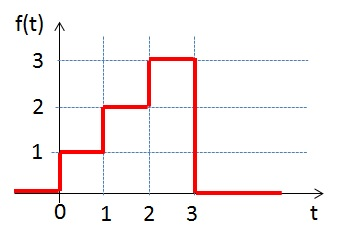
\includegraphics[scale=0.7]{images/Ex_Laplace_Fonction_marche_escalier.jpg} 	
	\end{minipage}
	\vspace{0.5\baselineskip}
	
	La fonction discontinue ci-dessus peut être exprimée sous la forme d'une somme de fonctions échelons. En repérant les instants de transition et les amplitudes des paliers, celle-ci s'écrit : $f(t)= u(t) + u(t-1) + u(t-2) - 3u(t-3)$.
	La transformée de Laplace étant linéaire, la transformée de Laplace de f(t) sera la somme des transformées de chaque terme de l'expression de f(t). En identifiant la transformée de Laplace de la fonction échelon et en appliquant le théorème du retard, on détermine l'expression de la transformée de Laplace de f(t) :
	\begin{equation*}
	F(p)=\mathcal{L}[f(t)]=\mathcal{L}[u(t)]+\mathcal{L}[u(t-1)]+\mathcal{L}[u(t-2)]-3\mathcal{L}[u(t-3)]
	\end{equation*}
	\begin{equation*}
	F(p)=\frac{1}{p}+\frac{e^{-p}}{p}+\frac{e^{-2p}}{p}-3\frac{e^{-3p}}{p}
	\end{equation*}
	\vspace{1\baselineskip}
		
	
	
	\section{Transformée de Laplace inverse}
	
	
	Du point de vue pratique, le but de la transformée de Laplace est de fournir un outil simple pour le calcul des réponses temporelles des systèmes linéaires. Elle permet de calculer la représentation fréquentielle d'une fonction à partir de sa représentation dans le domaine temporel. Dans le domaine fréquentiel, le calcul de la réponse du système est facilité en passant par la fonction de transfert. Cependant, si nous ne disposons pas d'une transformation mathématique permettant de réaliser le passage inverse, cette approche perd de son intérêt.  Fort heureusement, cet outil existe. Il s'agit de la transformée de Laplace inverse, que nous allons rapidement présenter. 
	 Elle permet de transformer une fonction définie dans le domaine des fréquences complexes p en une fonction définie dans le domaine temporel. Nous la noterons $\mathcal{L}^{-1}$. Comme la transformée de Laplace, la transformée de Laplace inverse est une fonction linéaire.
	
	
	\subsection{Méthode pratique d'utilisation}
	
	La transformée de Laplace inverse est donnée par la formule de Bromwich-Mellin , où $\sigma$ est choisi pour que l'intégrale converge.
	
	\begin{equation}\label{TL_inverse}
	f(t) = \mathcal{L}^{-1}[F(p)]=\frac{1}{2\pi j}\int_{\sigma - j\infty}^{\sigma + j\infty}F(p)exp(pt) \deriv p
	\end{equation}
	
	Dans la pratique, cette formule est difficile à mettre en œuvre car elle nécessite de calculer une intégrale dans le plan complexe. Ceci dépasse le cadre de ce cours et nous n'effectuerons pas de calcul de cette transformée. Dans ce cours, nous privilégierons la méthode utilisée en pratique, basée sur les tables reliant des fonctions courantes et leur transformée de Laplace, comme le tableau \ref{Tab:Transfo_Laplace_usuelle}. Il s'agit de rechercher des paires de transformées. A partir de la fonction F(p), on identifie des fonctions connues et on déduit la fonction temporelle correspondante. Dans le cas de fonctions compliquées, le calcul de la forme temporelle passe par des approches basées sur le calcul numérique, non détaillées ici. Dans de nombreux cas pratiques, les expressions des transformées de Laplace peuvent être données sous la forme d'une fraction rationnelle, pour laquelle on ne dispose pas directement de la fonction temporelle correspondante. Il est nécessaire de transformer d'abord l'expression de la transformée de Laplace avant d'identifier des formes courantes. On utilisera notamment une technique de décomposition en pôles et en résidus.
	 
	\subsection{Décomposition pôles-résidus}
	Comme nous l'avons dans la partie II.3, la plupart des transformées de Laplace peuvent être mises sous la forme d'une fonction rationnelle, rapport de deux polynômes faisant apparaitre leurs racines (pôles et zéros). Cependant, il n'existe sans doute pas une paire de transformées simples pour toutes les fonctions rationnelles. Pour appliquer la méthode précédente, il est nécessaire de décomposer cette fonction rationnelle en éléments plus simples, dont on connait la paire de transformées.
	Il est possible de montrer que toute fonction rationnelle de deux polynômes peut s'écrire sous la forme d'une somme d'éléments simples, appelées fractions partielles ne dépendant que des pôles et de constantes appelées résidus. Cette décomposition s'appelle la décomposition pôles-résidus, dont la forme est illustrée par \ref{Forme_decompo_pole_residu}. Cette décomposition ne fonctionne qu'avec des fractions dites "propres" pour lesquelles le nombre n de pôles est supérieur ou égal au nombre m de zéros. Dans ce cas, la fraction rationnelle peut se décomposer en n termes dont il faut déterminer les résidus $A_{n}$.
	
	\begin{equation}\label{Forme_decompo_pole_residu}
	F(p)=\frac{N(p)}{D(p)}=A\frac{(p-p_{zm})...(p-p_{z1})}{(p-p_{pn})...(p-p_{p1})}=\frac{A_{1}}{p-p_{p1}}+\frac{A_{2}}{p-p_{p2}}+...+\frac{A_{n}}{p-p_{pn}}
	\end{equation}
	
	On voit immédiatement l'intérêt de cette approche car on remarque qu'on identifie immédiatement la paire de transformée simple. En effet, la transformée de Laplace inverse de la fraction partielle est une fonction exponentielle, dépendante du pôle.
	
	\vspace{0.5\baselineskip}
	
	\textbf{\underline{Cas d'une fraction impropre (n < m) :}}
	
	Avant de voir comment réaliser cette décomposition pôles-résidus, traitons d'abord le cas des fractions impropres (plus de zéros que de pôles). La décomposition pôles-résidus n'est pas directe. Il est cependant possible d'exprimer cette fraction impropre comme la somme d'un terme (qui ne sera pas une fraction) et d'une fraction propre (\ref{reduction_fraction_impropre}). Il est indispensable que le premier terme ait une transformée de Laplace inverse connue.
	\begin{equation}\label{reduction_fraction_impropre}
	\frac{N(p)}{D(p)}=Q(p)+\frac{R(p)}{D(p)}~,~si~n<m
	\end{equation}
	
	 Q(p) n'est rien d'autre que le quotient de la division entre N(p) et D(p), tandis que R(p) est le reste. Cette décomposition consiste donc à faire une division entre deux polynômes. Illustrons-le par un exemple.
	 
	 \vspace{0.5\baselineskip}
	 \underline{Exemple :} décomposer la fonction $\frac{2p^{3}+p^{2}-4p}{p^{2}+p-2}$ pour faire apparaître une fraction propre.
	 
	 La division est décrite ci-dessous. Elle s'effectue comme suit : on identifie chaque terme du quotient afin d'éliminer le terme de plus haut degré du numérateur. Par exemple, le terme de plus haut degré de Q(p), 2p, est choisi de manière à éliminer $2p^{3}$ du numérateur. Comme il ne reste plus que $p^{2}$, le prochain terme de Q(p) est -1. Le calcul s'arrête ensuite. On a déterminé Q(p) et R(p).
	 
	 \begin{figure}[h!]
	 	\centering
	 	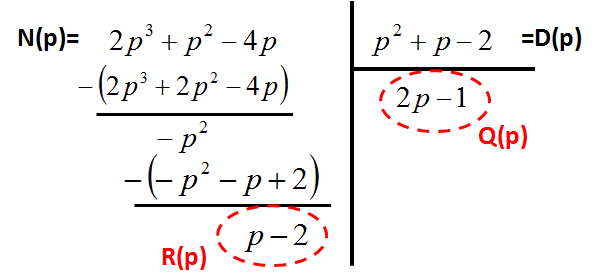
\includegraphics[scale=0.5]{images/ex_fraction_impropre.png} 
	 \end{figure}
 	
 	On peut donc écrire $\frac{2p^{3}+p^{2}-4p}{p^{2}+p-2}=(2p-1)+\frac{p-2}{p^{2}+p-2}=Q(p)+\frac{R(p)}{D(p)}$. Le terme $\frac{R(p)}{D(p)}$ est une fraction propre, tandis qu'on peut associer à Q(p) une transformée de Fourier simple, en l'occurence $2tu(t)-\delta(t)$ (voir tableau \ref{Tab:Transfo_Laplace_usuelle}). \\
	
	
	Nous considérons maintenant que nous disposons d'une fraction propre. Voyons comment effectuer facilement la décomposition pôles-résidus. Un préalable consiste à disposer des zéros et des pôles de la fonction rationnelle, afin de pouvoir écrire l'égalité de l'équation \ref{reduction_fraction_impropre}. Il existe plusieurs méthodes de décomposition pôles-résidus, nous n'en mentionnerons que deux. 
	
	\subsubsection{Association des fractions partielles}
	La première méthode consiste à partir de la forme en fractions partielles, puis de les associer pour revenir à la forme initiale de la fonction rationnelle, mais exprimée avec les résidus. On obtient ainsi n équations où les n inconnues sont les résidus. Prenons l'exemple suivant, où les pôles sont égaux à 1 et -2 :
	\begin{equation*}
	\frac{p-2}{p^{2}+p-2}=\frac{A}{p-1}+\frac{B}{p+2}
	\end{equation*}
	On cherche les résidus A et B. En les associant, on obtient $\frac{p-2}{p^{2}+p-2}=\frac{A(p+2)+B(p-1)}{p^{2}+p-2}=\frac{(A+B)p+(2A-B)}{p^{2}+p-2}$. On détermine les résidus en résolvant le système d'équations suivants :
	\begin{equation*}
	\left \{
	\begin{array}{l l}
	A+B=1 \\
	2A-B=-2 \\
	\end{array}
	\right .
	\end{equation*}
	On trouve les solutions suivantes : $A=-\frac{1}{3}$ et $B=\frac{4}{3}$. Cette approche simple peut devenir fastidieuse lorsque le nombre de pôles s'accroit. 
	
	\subsubsection{Méthode du cache}
	
	Une méthode alternative est la méthode du cache. Elle consiste à annuler un pôle pour déterminer le résidu associé, et répéter l'opération pour chaque pôle. Par exemple, supposons que l'on cherche le résidu $A_{i}$ associé au pôle $p_{pi}$. On multiplie la fraction par $(p-p_{pi})$. Dans la fraction rationnelle, l'effet du pôle va disparaitre. En prenant $p=p_{pi}$, on fera disparaitre les autres fractions partielles et on isolera ainsi le résidu $A_{i}$. Pour l'illustrer, reprenons l'exemple précédent :
	\begin{equation*}
	\frac{p-2}{p^{2}+p-2}=\frac{p-2}{(p-1)(p+2)}=\frac{A}{p-1}+\frac{B}{p+2}
	\end{equation*}
		
	Commençons par déterminer le résidu A associé au pôle p=1. On multiplie la fraction rationnelle par (p-1) et on obtient :
	\begin{equation*}
	\frac{p-2}{(p+2)}=A+\frac{B(p-1)}{p+2}
	\end{equation*}
	En fixant p = 1, on détermine $A=\frac{1-2}{(1+2)}=-\frac{1}{3}$. On répète l'opération pour déterminer l'autre résidu associé au pôle p=-2. On multiplie la fraction rationnelle par (p+2) et on obtient :
	\begin{equation*}
	\frac{p-2}{(p-1)}=\frac{A(p+2)}{p-1}+B
	\end{equation*}
	En fixant p = -2, on détermine $A=\frac{-2-2}{(-2-1)}=\frac{4}{3}$. La décomposition pôles-résidus s'écrit donc :
	\begin{equation*}
	\frac{p-2}{p^{2}+p-2}=\frac{-1}{3(p-1)}+\frac{4}{3(p+2)}
	\end{equation*}
	Sous cette forme, on identifie facilement la transformée de Laplace inverse, qui est égale à $(-\frac{1}{3}e^{t}+\frac{4}{3}e^{-2t})u(t)$.
	
	
	\vspace{1\baselineskip}
	

	
	\section{Applications} 
	Nous allons présenter deux applications où l'utilisation de la transformée de Laplace et de son inverse trouve tout leur intérêt : 
	\begin{itemize}
		\item la résolution d'équations différentielles
		\item le calcul de la réponse transitoire de systèmes linéaires
	\end{itemize}
	
	\subsection{Résolution d'équations différentielles ordinaires}
	La transformée de Laplace constitue un outil puissant de résolution des équations différentielles ordinaires, qui ne dépendent que d'une variable. De manière générale, elles peuvent s'écrire sous la forme suivante :
	\begin{equation}\label{key}
	L[t,x(t)]=f(t)
	\end{equation}
	
	où x(t) est l'inconnue, L un opérateur linéaire quelconque (superposition des effets d'opérateurs proportionnels, intégrateurs et différenciateurs) et f(t) une fonction quelconque. Dans le domaine des fréquences complexes, l'effet d'une dérivée et d'une intégration se résument à une multiplication et une division par la fréquence p. Ainsi, en passant dans le domaine fréquentiel, l'équation différentielle se transforme en une simple équation algébrique. En isolant le terme X(p) et en utilisant la transformée de Laplace inverse (à condition qu'elle existe), on pourra déterminer la solution x(t) de l'équation.
	
	\vspace{1\baselineskip}
	
	\textbf{\underline{Exemple :}} 
	
	soit l'équation différentielle suivante : $y"(t)+4y'(t)+4y(t)=0$, où y(t) est une fonction causale. On a les conditions initiales suivantes : $y(0^{+})=1$ et $y'(0^{+})=-2$. Résoudre l'équation différentielle.
	
	A l'aide du théorème de la dérivation, l'équation différentielle peut être exprimée dans le domaine de Laplace.
	\begin{equation*}
	p^{2}Y(p)-py(0^{+})-y'(0^{+})+4(pY(p)-y(0^{+}))+4Y(p)=0
	\end{equation*}
	En isolant Y(p) et en intégrant les valeurs des conditions initiales, on détermine l'expression de la solution Y(p) dans le domaine de Laplace.
	\begin{equation*}
	(p^{2}+4p+4)Y(p)=y'(0^{+})+(p+4)y(0^{+})
	\end{equation*}
	\begin{equation*}
	Y(p)=\frac{y'(0^{+})+(p+4)y(0^{+})}{p^{2}+4p+4}=\frac{p+2}{(p+2)^{2}}=\frac{1}{p+2}
	\end{equation*}
	On identifie sans difficulté la fonction temporelle associée à cette transformée de Laplace à l'aide du tableau \ref{Tab:Transfo_Laplace_usuelle}.
	\begin{equation*}
	y(t)=\mathcal{L}[Y(p)]=e^{-2t}u(t)
	\end{equation*}
	On vérifie que cette solution satisfait bien aux conditions initiales fixées et est une solution de l'équation différentielle.
	
	
	\vspace{1\baselineskip}
	
	\subsection{Calcul de la réponse transitoire d'un système linéaire}
	
	\begin{figure}[h!]
		\centering
		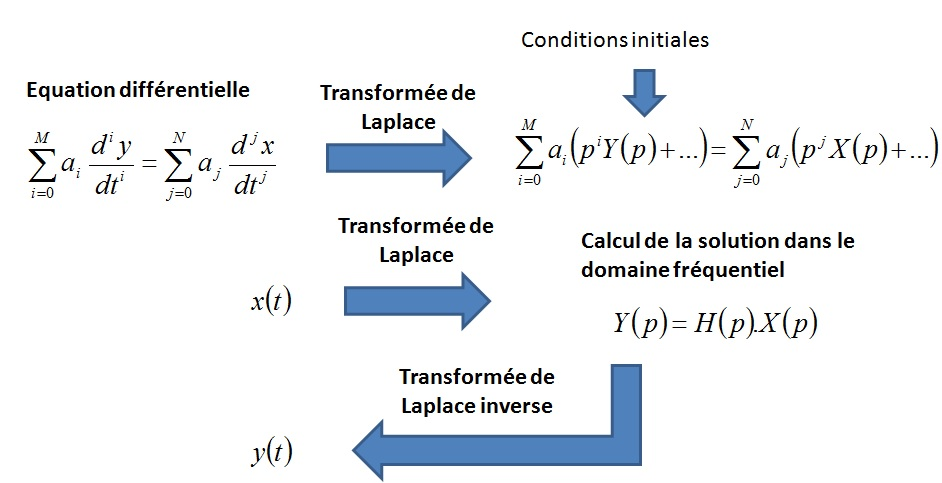
\includegraphics[scale=0.6]{images/Methodo_reso_equa_diff_Laplace.jpg}
		\caption{Méthodologie de résolution d'une équation différentielle ordinaire basée sur la transformée de Laplace}	
		\label{Fig:Methodo_reso_equa_diff_Laplace} 
	\end{figure}
	
	
	Comme nous l'avons vu avec l'équation générale du système linéaire (\ref{equation_generale_LTI}), le comportement transitoire d'un système est dicté par une équation différentielle. Déterminer la réponse temporelle à une excitation donnée revient à résoudre cette équation différentielle. Le problème est donc équivalent au précédent et la transformée de Laplace constitue encore un outil de résolution adapté à ce genre de problème. Supposons que nous disposions de la fonction de transfert H(p) du système et que l'on recherche la réponse y(t) à une excitation x(t) dont l'expression est donnée. La première étape consiste à déterminer la transformée de Laplace X(p) de l'excitation. La réponse du système dans le domaine fréquentiel Y(p) est directement le produit de la fonction de transfert et de l'excitation X(p). Ensuite, la transformée de Laplace inverse de Y(p) permet de retrouver l'expression de la réponse temporelle y(t).
	Il est bien entendu indispensable de prendre en compte les conditions initiales du système, qui vont intervenir dans la réponse naturelle du système. Si l'expression de la fonction de transfert ne les intègre pas, il est indispensable de repartir de l'équation différentielle décrivant le système et établir la fonction de transfert en intégrant l'effet des conditions initiales. La méthodologie de calcul est résumée à la figure \ref{Fig:Methodo_reso_equa_diff_Laplace}.
	
	\vspace{1\baselineskip}
	
	
	\textbf{\underline{Exemple : réponse d'un circuit RC à un échelon}}
	
	On reprend l'exemple du circuit RC (passe haut) vu dans le chapitre précédent, pour lequel nous avions calculé la réponse harmonique. Le circuit est présenté ci-dessous.
	On considère qu'il est excité par un échelon d'amplitude E en t = 0, et que le condensateur est initialement chargé (la tension initiale à ses bornes est notée $U_{C0}$). On souhaite déterminer la réponse du circuit, correspondant à la tension aux bornes de la résistance.

	\begin{figure}[h!]
	\centering
	\begin{minipage}[c]{0.4\linewidth}
		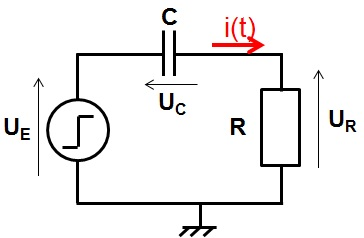
\includegraphics[scale=0.6]{images/circuit_RC_reponse_indicielle.jpg}
	\end{minipage} \hfill
	\begin{minipage}[c]{0.50\linewidth}
		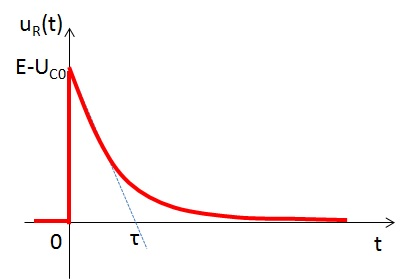
\includegraphics[scale=0.6]{images/reponse_RC_indicielle.jpg} 	
	\end{minipage}
	\caption{Circuit RC étudié (à gauche) et réponse à un échelon (à droite)}	
	\label{Fig:Circuit_RC_Laplace_inverse} 
	\end{figure}

	L'excitation du circuit s'écrit : $u_{E}(t)=Eu(t)$. Dans le domaine de Laplace, elle s'exprime : $U_{E}(p)=\frac{A}{p}$.
	Dans le chapitre précédent, nous avions déterminé l'équation différentielle liant l'excitation et la réponse du circuit. Nous allons la reprendre pour déterminer non seulement la fonction de transfert du circuit, mais aussi intégrer la condition initiale sur la charge du condensateur. On note $\tau=RC$ la constante de temps du circuit.
	\begin{equation}\label{}
	\frac{dU_{E}}{dt}=\frac{U_{R}}{RC}+\frac{dU_{R}}{dt}=\frac{U_{R}}{\tau}+\frac{dU_{R}}{dt}
	\end{equation}
	Le passage dans le domaine de Laplace de cette équation différentielle donne :
	\begin{equation*}
	pU_{E}(p)-U_{E}(0^{+})=\frac{U_{R}(t)}{\tau}+pU_{R}(p)-U_{R}(0^{+})
	\end{equation*}
	\begin{equation*}
	(p+\frac{1}{\tau})U_{R}(p)+U_{E}(0^{+})-U_{R}(0^{+})=pU_{E}(p)
	\end{equation*}
	En remarquant que $U_{E}(0^{+})-U_{R}(0^{+})$ est équivalent à la tension initiale $U_{C}(0^{+})=U_{C0}$ aux bornes du condensateur, l'équation s'écrit sous la forme ci-dessous. Le premier terme correspond à l'effet de l'excitation "filtré" par la fonction de transfert du circuit. Le second terme est lié à la présence d'une charge initiale aux bornes du condensateur.
	\begin{equation*}
	U_{R}(p) = \frac{p}{p+\frac{1}{\tau}}U_{E}(p)-\frac{1}{p+\frac{1}{\tau}}U_{C}(0^{+})=H(p)U_{E}(p)-\frac{1}{p+\frac{1}{\tau}}U_{C0}
	\end{equation*} 
	En intégrant l'expression de l'excitation, puis en effectuant la transformée de Laplace inverse, on détermine la réponse du circuit (\ref{reponse_RC_echelon}). Son tracée est présenté à la figure \ref{Fig:Circuit_RC_Laplace_inverse}.
	\begin{equation*}
	u_{R}(t)=\mathcal{L}^{-1}[H(p)U_{E}(p)]-\mathcal{L}^{-1}[\frac{1}{p+\frac{1}{\tau}}U_{C0}]
	\end{equation*}
	\begin{equation*}
	u_{R}(t)=E\mathcal{L}^{-1}[\frac{1}{p+\frac{1}{\tau}}]-U_{C0}\mathcal{L}^{-1}[\frac{1}{p+\frac{1}{\tau}}]
	\end{equation*}
	\begin{equation}\label{reponse_RC_echelon}
	u_{R}(t)=(E-U_{C0})e^{-\frac{t}{\tau}}u(t)=(E-U_{C0})e^{-\frac{t}{RC}}u(t)
	\end{equation}
	
	\vspace{1\baselineskip}
	

	
	\section{Exercices}
	
	\subsubsection{Exercice 1}
	
	Déterminez les transformées de Laplace des fonctions suivantes :
	
	a. $x(t)=e^{-2t}u(t-1)$
	
	b. $y(t)=e^{-2(t-1)}u(t-1)$
	
	c. $z(t) = \sqrt{2}cos(t+\frac{\pi}{4})$
	
	\begin{figure}[h!]
		\centering
		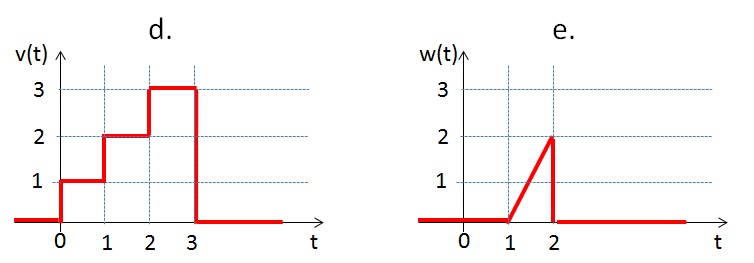
\includegraphics[scale=0.5]{images/Exo_2_1_a.jpg} 
	\end{figure} 
	
	\begin{figure}[h!]
		\centering
		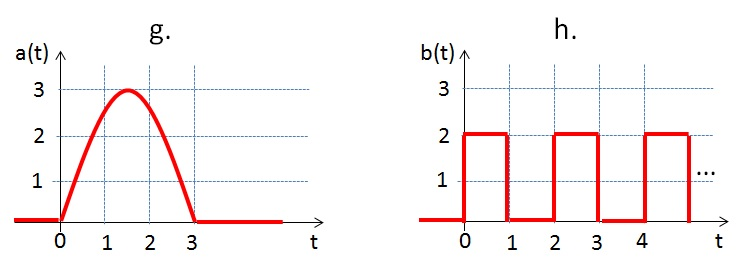
\includegraphics[scale=0.5]{images/Exo_2_1_b.jpg} 
	\end{figure}
	
	
	
	\vspace{1\baselineskip}
	
	\subsubsection{Exercice 2}
	
	Déterminez les expressions temporelles des fonctions suivantes :
	
	a. $X(p)=\frac{p-4}{p^{2}+16}$ 
	
	b. $Y(p) = \frac{p^{2}+3p+3-\frac{6}{p}}{p^{2}}$ 
	
	c. $Z(p) = \frac{p^{2}+4p+4}{p^{2}+2p+2}$
	
	d. $W(p) = \frac{p-1+e^{-p}}{p^{2}(1-e^{-p})}$. Tracez cette fonction.
	
	
	\vspace{1\baselineskip}
	
	\subsubsection{Exercice 3}
	
	Résoudre les équation différentielles suivantes :
	
	a. $x"+2x'+x=e^{-t}u(t)$, avec x(0) = 0 et x'(0) = 0. 
	
	b. $x"+6x'+8x=\delta(t)$ avec x(0)=1 et x'(0)=3. 
	
	\vspace{1\baselineskip}
	
	
	\subsubsection{Exercice 4}
	
	On reprend l'exercice 8 du chapitre 2.

	
	\begin{figure}[h!]
		\centering
		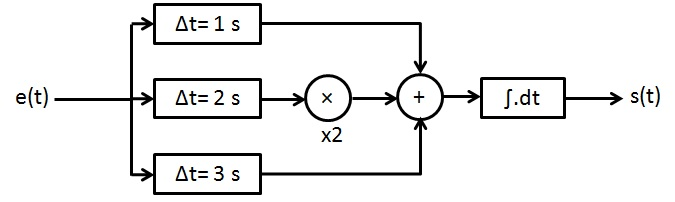
\includegraphics[scale=0.5]{images/Exo_2_6.jpg} 
	\end{figure}
	
	a. Ecrivez la fonction de transfert du système dans le domaine de Laplace.
	
	b. Calculez la réponse indicielle du système. On supposera que les conditions initiales de tous les nœuds internes du système sont nulles. 
	
	
	\vspace{1\baselineskip}
	
	\subsubsection{Exercice 5}
	
	On considère un circuit électrique, dont le courant i(t) est donné par l'équation ci-dessous.
	\begin{equation*}
	e(t)=\frac{d^{2}i}{dt^{2}}+7\frac{di}{dt}+10i(t)
	\end{equation*}
	On considère l'excitation suivante $e(t)=6e^{-3t}u(t)$. Les conditions initiales du circuit sont : $i(0) = 3~A$ et $\frac{di}{dt}(0)=3~A/s$.
	
	
	a. Etablir l'expression du courant dans le domaine de Laplace.
	
	b. En déduire l'expression temporelle du courant i(t).
	
	c. Vérifiez, en utilisant les expressions du courant dans le domaine de Laplace, puis dans le domaine temporel, que la condition initiale du courant est respectée. Déterminez ensuite les conditions finales. 
	
	\vspace{1\baselineskip}
	
	\subsubsection{Exercice 6 - Réponse d'un moteur à courant continu à aimants permanents}
	
	Le fonctionnement d'un moteur est gouverné par un modèle électromécanique, se présentant sous la forme de plusieurs équations différentielles reliant grandeurs électriques et mécaniques. Dans cet exercice, nous allons étudier le modèle simplifié d'un moteur à courant continu à aimants permanents. La figure ci-dessous présente le modèle électrique équivalent de l'induit. Celui-ci est modélisé par un circuit RL et est excité par une tension de commande notée $U_{C}$. Lorsque le moteur tourne, une force contre électromotrice (fcem) E est induite, qui est proportionnelle à la vitesse angulaire du moteur $\Omega$. 
	\begin{figure}[h!]
		\centering
		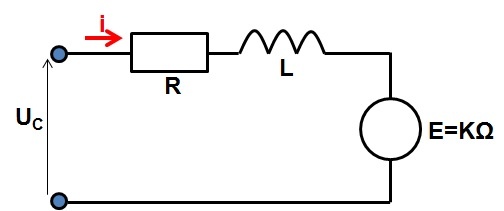
\includegraphics[scale=0.5]{images/Exo3_moteur.jpg} 
	\end{figure}	
	Le courant i circulant dans l'induit produit un couple moteur $C_{m}$, selon la même constante de proportionnalité K que celle liant la fcem et la vitesse de rotation du moteur. A ce couple moteur s'opposent plusieurs sources de couples résistants $C_{R}$ :
	\begin{itemize}
		\item l'inertie du moteur, donnée par le moment d'inertie J
		\item les frottements visqueux, caractérisés par le coefficient de frottement visqueux f
	\end{itemize}
	L'équation mécanique du moteur s'écrit alors :
	\begin{equation*}
	C_{m} = C_{R} = J\frac{d\Omega}{dt}+f\Omega
	\end{equation*}	
	Nous cherchons à déterminer la vitesse de rotation du moteur en fonction de l'excitation appliquée.
	Dans cet exercice, on considèrera les valeurs suivantes : r=0.2 $\Omega$, L = 0.2 mH, K = 0.057 N.m/A, J = $650.10^{-7}~kg.m^{2}$, f = $2.3.10^{-5}~N.m/rad.s^{-1}$. On suppose que le moteur est initialement à l'arrêt.\\
	
	a. Etablir l'équation différentielle reliant la vitesse de rotation et l'excitation $U_{C}$ du moteur.
	
	b. Déterminez la fonction de transfert du moteur dans le domaine de Laplace. Exprimez-la sous la forme $\frac{G}{p^{2}+2\alpha p+\omega_{0}^{2}}$.
	
	c. Calculez les pôles du système. Est-il stable ?
	
	d. En t = 0, on applique une commande de type échelon unitaire d'amplitude $Uc_{0}$ = 10 V. Déterminez l'expression du profil temporel de la vitesse angulaire.
	
	e. Esquissez le profil temporel de la vitesse angulaire. En régime permanent, quelle est la valeur de la vitesse ? 
	
		
	\newpage
	
\cleardoublepage
\chapter{Filtrage}

	Un filtre est un dispositif visant à modifier le contenu fréquentiel d'un signal. Une utilisation courante est de supprimer d'un signal des composantes fréquentielles indésirables (ou, inversement, d'extraire de ce signal certaines composantes utiles). La figure \ref{Fig:Effet_filtre_bruit} illustre ce type d'utilisation. Le graphique à gauche présente un signal digital corrompu par un bruit aléatoire important. La présence de ce bruit est indésirable, car il risque de corrompre l'interprétation de ce signal. Afin d'éviter toute erreur de décodage de ce signal, un filtre doit être synthétisé pour supprimer ce bruit, sans trop affecter le signal utile. L'utilisation d'un filtre est possible si le signal utile et le bruit occupent des bandes de fréquence différentes. Un outil d'analyse du signal, comme la transformée de Fourier que nous aborderons dans le prochain chapitre, permet de déterminer l'occupation fréquentielle des signaux.
	
	Dans l'exemple ci-dessous, le signal utile à une fréquence de 2.5 Hz. Le spectre du signal bruité est présenté à la figure \ref{Fig:Effet_filtre_bruit_spectre}. Le spectre du signal utile se situe principalement en dessous de 100 Hz. Le bruit est large bande, mais présente quatre composantes spectrales importantes au-dessus de 100 Hz. Pour éliminer ce bruit, on dimensionne un filtre passe-bas d'ordre 2 avec une fréquence de coupure de 100 Hz. L'effet de ce filtre sur le signal est présenté sur la partie droite de la figure \ref{Fig:Effet_filtre_bruit}. La présence du bruit n'est quasiment plus discernable. Comme le confirme le spectre du signal filtré (\ref{Fig:Effet_filtre_bruit_spectre}), le filtre a fortement atténué le spectre au-dessus de 100 Hz. On peut remarquer que le filtre affecte aussi la forme du signal utile, mais cet effet reste négligeable et ne contribuera pas à une erreur d'interprétation du signal.  
	
	\begin{figure}[h]
		\centering
		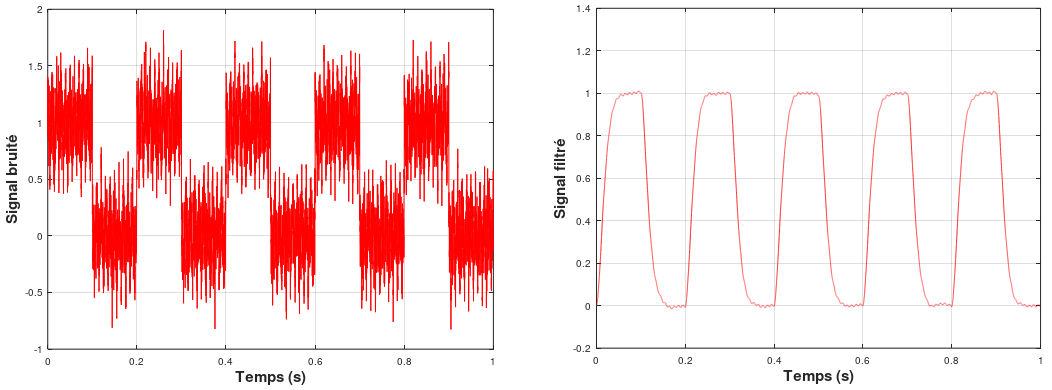
\includegraphics[scale=0.6]{images/Effet_filtre_bruit.png}
		\caption{Effet du filtre sur un signal bruité : signal bruite (à gauche) et filtré (à droite)}	
		\label{Fig:Effet_filtre_bruit} 
	\end{figure}

	\begin{figure}[h]
		\centering
		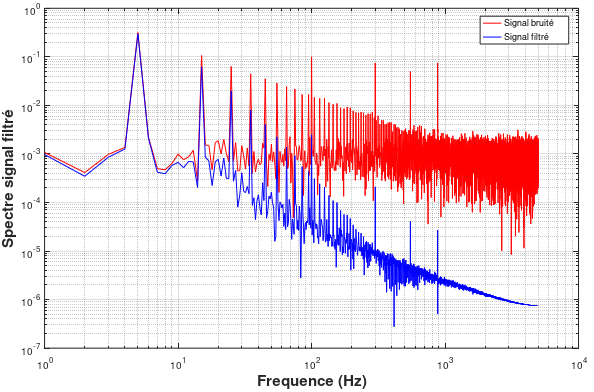
\includegraphics[scale=0.6]{images/Effet_filtre_bruit_spectre.png}
		\caption{Spectre du signal bruité et filtré}	
		\label{Fig:Effet_filtre_bruit_spectre} 
	\end{figure}
	
	
	Ce chapitre est dédié au filtre linéaire à temps invariant et leur analyse en régime harmonique. Les filtres n'ont aucune différence par rapport aux systèmes LTI vues précédemment. La différence vient de leur utilisation, qui nécessite une analyse dans le domaine fréquentiel. La connaissance de la fonction de transfert du filtre est donc centrale. En régime harmonique, nous la noterons H($\omega$) ou H(f).
	
	Dans ce chapitre, nous présenterons les outils et les termes usuels permettant de caractériser les filtres. Nous introduirons un outil d'analyse graphique : le diagramme de Bode et son tracé asymptotique.  
	

	
	\section{Définition d'un filtre}
	
	\subsection{Définition}
	
	Un filtre est un système, généralement passif, présentant une certaine sélectivité dans le domaine des fréquences. Il est utilisé pour atténuer (ou au contraire laisser passer) le signal sur une ou plusieurs bandes de fréquences.
	Il atténue ainsi certaines des composantes fréquentielles du signal d’entrée et en laisse passer d’autres, d’où son appellation de filtre ! C’est bien cette opération sélective d’atténuation ou d’amplification des fréquences que modélise la multiplication de l'excitation par la fonction de transfert.
	\begin{equation}\label{}
	Y(f) = H(f) \cdot X(f)
	\end{equation}

	Une manière pratique d'étudier un filtre est de l'analyser en régime harmonique, donc dans le domaine fréquentiel. Pour mettre en évidence l'effet du filtre, la fonction de transfert peut être écrite sous la forme module-argument :
	
	\begin{equation}\label{key}
	H(f) = |H(f)|exp(j~arg(H(f)))
	\end{equation}
	
	 Le module correspond au gain du filtre, c'est-à-dire le rapport entre les amplitudes de la réponse du filtre et de son excitation. Si le module est important, alors le signal d'entrée est faiblement atténué voire amplifié. Sinon, il est filtré.
	Si les signaux d'entrée et de sortie représentent le même type de grandeur (par exemple, une tension dans le cas de signaux électriques), le gain est sans unité.\\ 
	
	L'argument correspond au déphasage apporté par le filtre. Celui-ci traduit un retard $ \tau $ introduit par le filtre à la fréquence f, déterminé par l'équation \ref{retard}.	
	
	\begin{equation}\label{retard}
	\tau = \frac{d(Arg(H(f)))}{2\pi df}
	\end{equation}
	
	\vspace{1\baselineskip}
	
	\underline{\textbf{Filtre à phase linéaire}}
	
	On remarque une propriété intéressante : soit un signal constitué de la superposition de plusieurs signaux sinusoïdaux, traverante un filtre présentant un déphasage variable en fonction de la fréquence. Même si le gain est le même à ces différentes fréquences, si le retard introduit par le filtre varie avec la fréquence, alors le signal en sortie présentera une distorsion. Ceci démontre qu'il ne faut pas négliger l'information de phase d'un filtre.
	Pour éviter cette distorsion, il est nécessaire que le retard soit constant. D'après \ref{retard}, cela est vérifié uniquement si le déphasage varie linéairement avec la fréquence. On parle alors de filtres à phase linéaire.
	
	On peut aussi remarquer qu'un filtre présentant un déphasage constant quelle que soit la fréquence ne doit pas être réalisable en pratique. En effet, celui-ci ne présenterait aucun retard. La sortie changerait simultanément avec l'entrée, ce qui est physiquement impossible.
	
	\vspace{1\baselineskip}
	
	\subsection{Filtre à réponse impulsionnelle réelle}
	Considérons le cas particulier, mais pratique, où la réponse impulsionnelle est une fonction réelle : $ \forall t \in \mathbb{R},~h(t) \in \mathbb{R}$. Une réponse temporelle prenant des valeurs complexes n’aurait pas directement de sens physique ! On peut alors appliquer la propriété suivante de la Transformée de Fourier : la Transformée de Fourier d’une fonction réelle est une fonction en général complexe mais admettant une symétrie conjuguée : $\forall f \in \mathbb{R},~H^{*}(f) = H(-f)$, c'est-à-dire dont le module est une fonction paire tandis que l’argument est une fonction impaire, comme le montre l'équation ci-dessous. 
	
	\begin{equation}\label{key}
	\forall f \in \mathbb{R},~|H(f)| = |H(-f)| ~~et~~arg(H(f)) = -arg(H(-f))
	\end{equation}
	
	\begin{figure}[h]
		\centering
		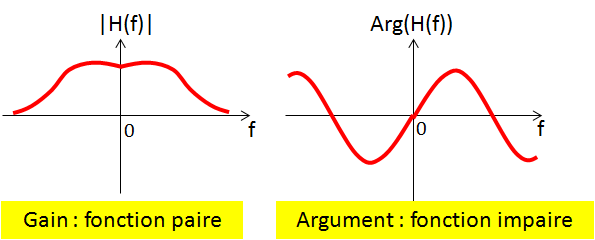
\includegraphics[scale=0.6]{images/symetrie_filtre_reel.png}
		\caption{Symétries du module et de l'argument d'un filtre réel}	
		\label{Fig:symetrie_filtre_reel} 
	\end{figure}
	 
	
	\subsection{Fréquence négative}
	
	Comme nous l'avons vu dans les chapitres précédents, la fréquence est une grandeur réelle pouvant être négative. En raison de propriétés de symétries introduites par la transformée de Fourier pour les fonctions réelles, les représentations que nous utiliserons dans ce chapitre ne font apparaître que les fréquences positives. Les fréquences négatives sont omises par convention parce qu'elles n'apportent pas d'informations supplémentaires : le gain est une fonction paire tandis que le déphasage est une fonction impaire.
	
	La notion de basse ou de haute fréquence ne s’attache qu’à la valeur absolue de la fréquence considérée : seules les fréquences positives f appartenant à $\mathbb{R}^{+}$ ont un sens physique ; les fréquences négatives f appartenant à $\mathbb{R}^{-}$ n’ont pas de signification physique directe, mais leur prise en compte assure une utilisation correcte de l’analyse harmonique comme outil d’étude des filtres.
	
	Ainsi, la convention pratique veut que le tracé des caractéristiques des gains et déphasage des filtres (diagramme de Bode), la définition des fréquences de coupure et des bandes passantes soient uniquement donnés dans le domaine des fréquences positives. Ils existent aussi pour les fréquences négatives, mais sont obtenus facilement par symétrie.
	
	\vspace{1\baselineskip}
	
	\section{Analyse harmonique}
	A partir de la connaissance du gain et du déphasage de la fonction de transfert, lorsque le filtre est attaqué par un signal (co)sinusïdal, il est très simple de déterminer l'expression de sa réponse. En considérant une notation complexe, la réponse temporelle du filtre en régime harmonique est donnée par :
	\begin{equation}\label{}
	x(t) = Re[X_{0}exp(j\Phi_{x})exp(j2\pi ft)] \Rightarrow y(t) = Re[X_{0}|H(f)exp(j(\Phi_{x}+arg(H(f))))exp(j2\pi ft)]
	\end{equation}
	Celle-ci peut aussi s'écrire sous la forme suivante :
	\begin{equation}\label{key}
	x(t) = X_{0}cos(2\pi ft+\Phi_{x}) \Rightarrow y(t) = X_{0}|H(f)+cos(2\pi ft+\Phi_{x}+arg(H(f)))
	\end{equation}
	
	\section{Représentation - Diagramme de Bode}
	\subsection{Diagramme de Bode}
	En régime harmonique, l'étude d'un filtre passe par une analyse de son gain et de son déphasage. Il faut donc chercher une représentation graphique adaptée à l'analyse du comportement fréquentiel du filtre. La méthode la plus courante est le tracé du diagramme de Bode. Il contient deux tracés graphiques décrivant :
	\begin{itemize}
		\item l'évolution du gain en fonction de la fréquence
		\item l'évolution du déphasage en fonction de la fréquence
	\end{itemize}

	\vspace{0.5\baselineskip}

	Bien qu'il n'existe pas une forme de représentation unique du diagramme de Bode, certains usages sont récurrents et il convient de les expliquer. Pour des raisons pratiques, l'axe fréquentiel est généralement tracé en échelle logarithmique. En général, on s'intéresse au comportement fréquentiel sur une large gamme de fréquence, couvrant plusieurs décades. Un tracé avec une échelle linéaire offre une résolution constante, qui cache les détails dans les basses fréquences. Avec un tracé en échelle logarithmique, la résolution varie en fonction de la fréquence et s'adapte à chaque décade. Le même niveau de détail peut être apprécié en basse ou en haute fréquence. C'est ce qu'illustre la figure \ref{Fig:Effet_Flin_log} : le filtre étudié est de type passe-bas, c'est-à-dire qu'il laisse passer les signaux basses fréquences. Le tracé est réalisé entre 100 Hz et 1 MHz. Avec l'échelle linéaire, le tracé ne permet pas d'évaluer précisément à partir de quelle fréquence le filtre commence à atténuer significativement le signal d'entrée. Avec l'échelle logarithmique, on peut mieux évaluer cette fréquence, appelée fréquence de coupure, qui se situe aux alentours de 1 kHz.
	\begin{figure}[h]
		\centering
		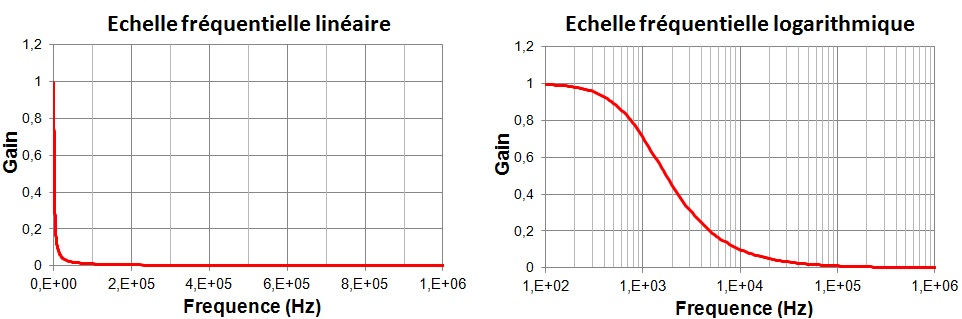
\includegraphics[scale=0.6]{images/Effet_Flin_log.jpg}
		\caption{Tracé du gain de la fonction de transfert d'un filtre passe-bas : échelle fréquentielle linéaire (à gauche) et logarithmique (à droite)}	
		\label{Fig:Effet_Flin_log} 
	\end{figure}
	
	\textbf{\underline{Conseil pratique : comment tracer une échelle logarithmique ?}}
	
	On définit tout d'abord le pas représentant une décade (par exemple 2 cm par décade). On considère que l'origine est placé en f=1 (log10(1) = 0). La position de toute valeur par rapport à cette origine sera donnée par pas $\times log_{10}(valeur)$. Ainsi, la valeur 10 (une décade de plus que 1) sera située à 2 cm à droite de l'origine, 100 (deux décades de plus) sera située à 4 cm à droite de l'origine, tandis que 0.1 (une décade de moins) sera située à 2 cm à gauche de l'origine. Par exemple, la valeur 50 sera située à $2\times log10(50)$ = 3.4 cm à droite de l'origine.\\
	
	Une autre convention consiste à exprimer les gains en décibels (\ref{dB}), qui n'est rien d'autre qu'une représentation des valeurs sur une échelle logarithmique. De part leur sélectivité en fréquence, les gains des filtres vont présenter des valeurs très variables en fonction de la fréquence. Pour les mêmes raisons que la représentation des fréquences, une échelle logarithmique pour le gain permettra d'apprécier avec la même résolution les faibles et les fortes valeurs de gain. La figure \ref{Fig:Effet_Ylin_dB} l'illustre, en reprenant l'exemple du tracé du gain du filtre précédent. Le tracé du gain sur une échelle linéaire ne permet pas de le mesurer précisément lorsqu'il atteint de faibles valeurs. A contrario, lorsqu'il est exprimé en dB, la mesure des faibles valeurs devient plus précise, mettant en évidence les tendances particulières du gain. Par exemple, le gain de ce filtre décroit avec une pente de -20 dB par décade au-dessus de la fréquence de coupure, ce qui est typique d'un filtre passe-bas d'ordre 1. 
	\begin{equation}\label{dB}
	G_{dB} = 20 \cdot log(|H(f)|)
	\end{equation}
	
	\begin{figure}[h!]
		\centering
		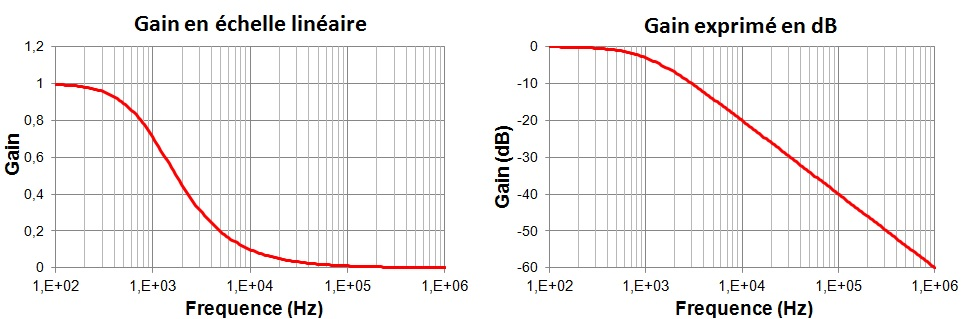
\includegraphics[scale=0.6]{images/Effet_Ylin_dB.jpg}
		\caption{Tracé du gain de la fonction de transfert d'un filtre passe-bas : échelle linéaire (à gauche) et en décibel (à droite)}	
		\label{Fig:Effet_Ylin_dB} 
	\end{figure}
	
	\begin{minipage}[l]{0.4\linewidth}
		Il n'y a pas de convention particulière pour le déphasage, qui peut être exprimé en radians ou en degrés. La figure ci-contre présente le diagramme de Bode du filtre précédent, montrant les tracés de l'évolution fréquentielle de son gain et de son déphasage. Le diagramme de Bode indique un déphasage dont la valeur diminue entre 0 et $-\frac{\pi}{2}$. Le déphasage étant négatif, le filtre introduit un retard.	
	\end{minipage} \hfill
	\begin{minipage}[c]{0.50\linewidth}
			%\centering
			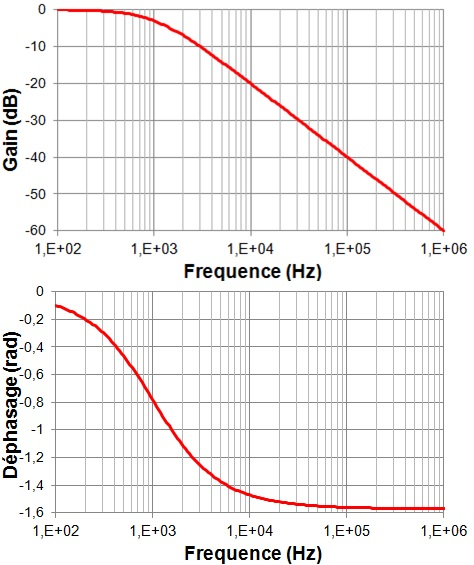
\includegraphics[scale=0.6]{images/Bode_passe-bas.jpg}
			%\caption{Diagramme de Bode d'un filtre passe-bas}	
			%\label{Fig:Bode_passe-bas} 	
	\end{minipage}

	\vspace{1\baselineskip}

		\textbf{\underline{Remarque : normalisation des fréquences :}}
	
	Un filtre de nature donnée présentera toujours la même tendance fréquentielle. Seule la ou les fréquences de coupure changeront selon les propriétés du filtre. Pour disposer d'une représentation indépendante de la fréquence de coupure, il est courant de représenter l'axe des fréquences sous la forme d'une fréquence normalisée. Cette normalisation se fait par rapport à une fréquence de référence, généralement la fréquence coupure du filtre. Ainsi, le même gabarit peut être utilisé pour plusieurs filtres présentant différentes fréquences de coupure. Si l'axe fréquentiel est exprimé en pulsation, la normalisation se fera de la même manière.
	\begin{equation}\label{key}
	f_{norm} = \frac{f}{f_{c}}
	\end{equation}
	\begin{equation}\label{key}
	\omega_{norm} = \frac{\omega}{\omega_{c}}
	\end{equation}
	
	\begin{figure}[h!]
		\centering
		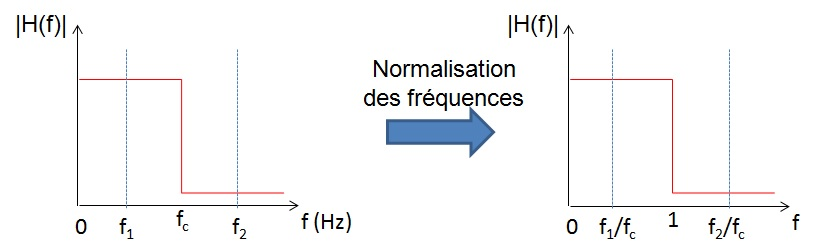
\includegraphics[scale=0.6]{images/freq_norm.jpg}
		\caption{Normalisation des fréquences}	
		\label{Fig:freq_norm} 
	\end{figure}
	

	
	
	\subsection{Tracé asymptotique du diagramme de Bode}
	
	Les fonctions de transfert des filtre linéaires peuvent souvent être écrites sous la forme d'un rapport de deux polynômes, comme le montre l'équation \ref{TF_usuelle_filtre}. Comme nous allons le voir, cette forme particulière facilite le tracé graphique du module de la fonction de transfert, sous une forme appelée tracé asymptotique. Celui-ci permet de visualiser ou représenter sans calculs compliqués l'évolution du module, les pentes, les points d'inflexion (fréquences de coupure) ou l'ordre du filtre. Il s'agit d'un outil d'ingénierie couramment utilisé, soit dans la synthèse de filtre comme moyen de définir le gabarit d'un filtre, ou bien de son analyse à partir de l'expression de sa fonction de transfert. 
	\begin{equation}\label{TF_usuelle_filtre}
	H(\omega)=G\frac{\prod_{i=1}^{m}(1+j\frac{\omega}{\omega_{i}})}{\prod_{j=1}^{n}(1+j\frac{\omega}{\omega_{j}})}
	\end{equation}
	
	Le tracé asymptotique est une représentation simplifiée du module, même s'il peut s'étendre à celui de la phase. Il consiste à représenter le comportement asymptotique de chacun des termes des produits au numérateur et au dénominateur de l'équation \ref{TF_usuelle_filtre}, où G est une constante réelle, $\omega_{i}$ représente les zéros et $\omega_{j}$ les pôles de la fonction de transfert. La représentation se fait systématiquement sur un graphique aux échelles log-log, avec l'utilisation de décibels sur l'axe des ordonnées. De cette manière, les termes de l'équation \ref{TF_usuelle_filtre} présenteront des décroissances linéaires en +/- 20 dB/dec. En outre, les produits et les divisions se transformeront en addition ou en soustraction, opérations plus simples (on rappelle que $log(a \cdot b)=log(a)+log(b)$ et log($\frac{a}{b})=log(a)-log(b)$).
	
	Nous allons illustrer le tracé asymptotique du module et de la phase d'une fonction de transfert quelconque. Mais avant, nous allons réaliser ceux des termes de base de l'équation \ref{TF_usuelle_filtre}. Dans les différents exemples, nous allons considérer une pulsation de coupure $\omega_{i} = 100~rad/s$. Commençons par le terme $j\omega$. C'est un cas particulier où la racine est nulle. Après passage en décibels, son module devient $20log(\omega)$. 
	
	
	\begin{minipage}[l]{0.5\linewidth}
		Dans un tracé log-log, comme celui présenté ci-contre, le module évolue linéairement avec une pente en 20 dB/décade.  Le terme inverse, $\frac{1}{j\omega}$, est très proche. Le passage en décibel conduit à : $20log(\frac{1}{j\omega})=20log(1)-(20log(\omega)=-20log(\omega)$. L'évolution se fait aussi linéairement, mais avec une croissance en -20 dB/dec. Dans ce cas, le tracé asymptotique est évident, puisqu'il consiste en une simple droite de pente égale à +/-20 dB/dec. Ces deux termes étant purement imaginaires, leur phase est de $+\frac{\pi}{2}$ pour le premier terme, $-\frac{\pi}{2}$ pour le second.
	\end{minipage} \hfill
	\begin{minipage}[c]{0.50\linewidth}
		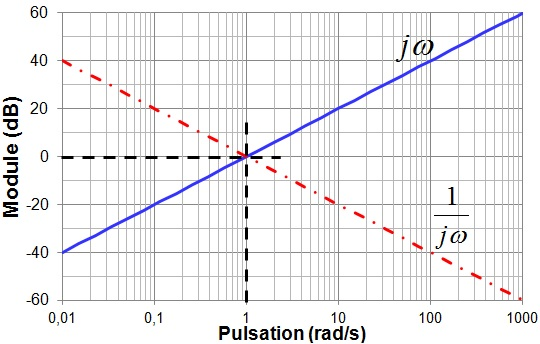
\includegraphics[scale=0.6]{images/Trace_asympt_jw.jpg}	
	\end{minipage}

	\vspace{1\baselineskip}
	
	\begin{minipage}[l]{0.5\linewidth}
		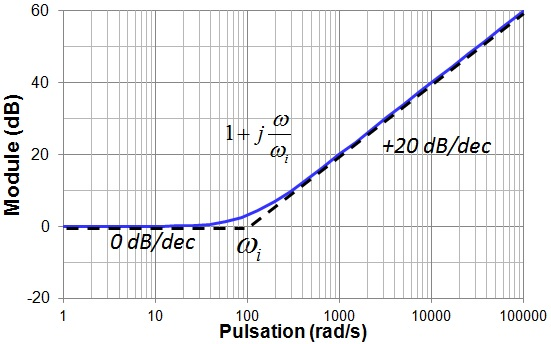
\includegraphics[scale=0.6]{images/Trace_asympt__1_plus_jw.jpg}
	\end{minipage} \hfill
	\begin{minipage}[c]{0.50\linewidth}
		Considérons maintenant le terme $1+j\frac{\omega}{\omega_{i}}$.	Tant que la pulsation est inférieure à $\omega_{i}$, le module reste constant, proche de 1 (soit 0 dB). Par contre, au-delà de $\omega_{i}$, le module augmente linéairement avec la fréquence, en +20 dB/dec. Entre ces deux comportements asymptotiques, l'évolution fréquentielle est plus compliquée à tracer précisément. Néanmoins, en ramenant le tracé à deux droites de pente 0 et +20 dB/dec se coupant en $\omega_{i}$, on obtient une représentation simplifiée mais montrant précisément la fréquence de coupure et les tendances asymptotiques de la fonction de transfert en dessous et au-dessus de la fréquence de coupure.	
	\end{minipage}

	\begin{minipage}[l]{0.5\linewidth}
		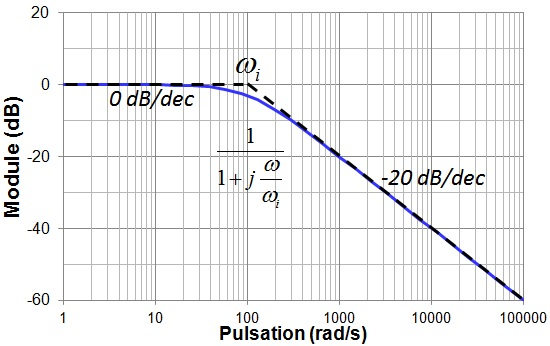
\includegraphics[scale=0.6]{images/Trace_asympt__1_moins_jw.jpg}
	\end{minipage} \hfill
	\begin{minipage}[c]{0.50\linewidth}
		De même, on peut représenter le tracé asymptotique du terme $\frac{1}{1+j\frac{\omega}{\omega_{i}}}$. Lors du passage en décibel, il devient : $20log(\frac{1}{1+j\frac{\omega}{\omega_{i}}}) = -20log(1+j\frac{\omega}{\omega_{i}})$. C'est donc le même terme que précédemment, mais au signe près. 	
	\end{minipage}
	
	\vspace{0.5\baselineskip}
	
	La phase de ces deux termes est égale à $+/-arctan(\frac{\omega}{\omega_{i}})$. On peut aussi en déduire deux comportements asymptotiques. Tant que la pulsation est largement inférieure à $\omega_{i}$, c'est la partie réelle qui domine donc la phase est proche de 0. Dès que la pulsation est bien plus grande que $\omega_{i}$, c'est la partie imaginaire et la phase tend vers $+/-\frac{\pi}{2}$. C'est ce qu'illustre la figure ci-dessous. On remarque le passage par $+/-\frac{\pi}{4}$ au passage par $\omega_{i}$.
	
	\begin{figure}[h!]
		\centering
		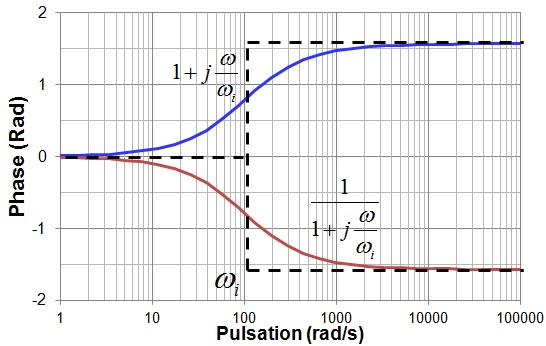
\includegraphics[scale=0.6]{images/Trace_asympt_phase_1_plus_jw.jpg}
	\end{figure}

	La multiplication des termes précédents par une constante réelle G, dans un diagramme de Bode en échelle log-log, introduit un simple décalage vertical du tracé égal à 20log(G) sans introduire de déphasage supplémentaire.
		
	\begin{minipage}[l]{0.5\linewidth}
		Il est possible qu'une racine soit multiple. Si elle apparait k fois, on verra un terme du type $(1+j\frac{\omega}{\omega_{i}})^{k}$ dans la fonction de transfert. Le passage en décibel de ce terme donne : $20log((1+j\frac{\omega}{\omega_{i}})^{k})=20k\cdot log(1+j\frac{\omega}{\omega_{i}})$. On retrouve donc le même genre de tracé asymptotique qu'au-dessus, mais le rythme de croissance (ou de décroissance) du module au-dessus de la fréquence de coupure est de +20xk dB/dec. Dans le cas d'une racine double, la pente sera de 40 dB/dec; 60 dB/dec pour une racine triple ... Dans l'exemple ci-contre, on considère une racine double. Ci-dessous, la phase de ce terme est tracé. Comme précédemment, on observe deux tendances asymptotiques : une phase tendant vers 0 en-dessous de $\omega_{i}$, puis une phase tendant vers $pi$ au-dessus de $\omega_{i}$. Dans le cas où la racine apparaît k fois, le déphasage tendra vers $k \cdot \frac{\pi}{2}$.	
	\end{minipage} \hfill
	\begin{minipage}[c]{0.50\linewidth}
		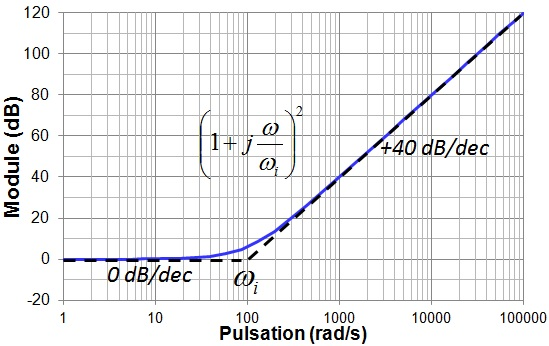
\includegraphics[scale=0.6]{images/Trace_asympt__1_plus_jw_carre.jpg}	
	\end{minipage}
	
	\vspace{1\baselineskip}
	
	\begin{figure}[h!]
		\centering
		\includegraphics[scale=0.6]{images/Trace_asympt_phase_1_plus_jw_carre.jpg}
	\end{figure}
	
	Nous n'avons considéré que des cas particuliers de fonctions de transfert relativement simple. Comment faire lorsque l'expression de la fonction de transfert présente plusieurs termes au numérateur et au dénominateur. Là encore, le tracé dans un graphe log-log simplifie grandement les choses. Pour le tracé du module, après un passage en décibel, l'équation \ref{TF_usuelle_filtre} peut s'écrire sous la forme suivante. On retrouve les termes élémentaires vus précédemment. Le tracé asymptotique de cette fonction de transfert ne sera que l'addition des tracés asymptotiques individuels de chaque terme élémentaire. Si sur une plage de fréquence, deux termes ont une pente donnée, le comportement asymptotique résultant sera la somme de ces pentes. 
	
	\begin{equation}\label{}
	20log(H(\omega))=20log(G\frac{\prod_{i=1}^{m}(1+j\frac{\omega}{\omega_{i}})}{\prod_{j=1}^{n}(1+j\frac{\omega}{\omega_{j}})})=20log(G)+\sum_{i=1}^{m}20log(1+j\frac{\omega}{\omega_{i}})-\sum_{j=1}^{n}20log(1+j\frac{\omega}{\omega_{j}})
	\end{equation}
	
	De la même manière, la phase de la fonction de transfert sera obtenue en additionnant les déphasages introduits par chacun des termes élémentaires, comme le montre l'équation ci-dessous.
	\begin{equation}\label{key}
	arctan(H(\omega))=\sum_{i=1}^{m}arctan(\frac{\omega}{\omega_{i}})-\sum_{j=1}^{n}arctan(\frac{\omega}{\omega_{j}})
	\end{equation}
	
	Nous allons illustrer comment réaliser cette opération à travers un exemple. Considérons la fonction de transfert suivante :
	\begin{equation*}
	H(\omega) = 2\frac{j\omega(1+j\frac{\omega}{1000})}{1+j\frac{\omega}{10}}
	\end{equation*}
	
	
	La fonction de transfert est déjà mise sous une forme équivalente à l'équation \ref{TF_usuelle_filtre}. On identifie trois termes :
	\begin{enumerate}
		\item $2j\omega$
		\item $1+j\frac{\omega}{1000}=1+j\frac{\omega}{\omega_{2}}$
		\item $1+j\frac{\omega}{10}=1+j\frac{\omega}{\omega_{1}}$\\
	\end{enumerate}
	
	 On trace individuellement le comportement asymptotique de chaque terme. On commence par le tracé du module. Sur la figure \ref{Fig:Construction_trace_asympt_module}, le comportement asymptotique des trois termes est représenté. On repère les deux fréquences de transition $\omega_{1}$ et $\omega_{2}$. Sur les trois plages de fréquence ainsi délimitées, on additionne les morceaux des tracés asymptotiques. Entre $\omega_{1}$ et $\omega_{2}$, l'augmentation en 20 dB/dec du module liée au terme 1 est compensée par la décroissance due au terme 2. Le coefficient multiplicateur 2 conduit à un décalage de +6 dB du module.
	 
	 De la même manière, on réalise le tracé asymptotique de la phase. Le terme 1 introduit un déphasage constant de $\frac{\pi}{2}$. Le déphasage du terme 2 tend vers $\frac{\pi}{2}$ à l'infini, tandis que celui du terme 3 tend vers $-\frac{\pi}{2}$. Le résultat de la construction est présenté sur la figure \ref{Fig:Construction_trace_asympt_phase}.
	 
	 \begin{figure}[h!]
	 	\centering
	 	\includegraphics[scale=0.5]{images/Constr_trace_asympt_Module.jpg}
	 	\caption{Construction du tracé asymptotique du module de la fonction de transfert exemple}	
	 	\label{Fig:Construction_trace_asympt_module} 
	 \end{figure}
 
 	\begin{figure}[h!]
 		\centering
 		\includegraphics[scale=0.5]{images/Constr_trace_asympt_Phase.jpg}
 		\caption{Construction du tracé asymptotique de la phase de la fonction de transfert exemple}	
 		\label{Fig:Construction_trace_asympt_phase} 
 	\end{figure}
 
 	A titre de comparaison, le module et la phase de cette fonction de transfert sont tracés sur un diagramme de Bode. On vérifie que les tracés asymptotiques reflètent correctement les tendances du module et de la phase de la fonction de transfert.
 	
 	\begin{figure}[h!]
 		\centering
 		\includegraphics[scale=0.7]{images/Diag_Bode_Exemple_Octave.jpg}
 		\caption{Diagramme de Bode de la fonction de transfert exemple}	
 		\label{Fig:Diag_Bode_TF_exemple} 
 	\end{figure}
 
 	
	\vspace{1\baselineskip}


	\section{Les principales caractéristiques d'un filtre}
	Lorsqu'on analyse un filtre ou lorsqu'on cherche à le dimensionner, plusieurs caractéristiques sont étudiées. Celles-ci définissent le comportement fréquentiel global. Nous allons les définir ici. 
	
	\subsection{Gain}
	
	Le gain est le module de la fonction de transfert et varie donc avec la fréquence. Néanmoins, on peut spécifier une valeur unique, qui correspond généralement à la valeur maximale du gain.
	
	\subsection{Fréquence(s) de coupure}
	
	Elles correspondent aux fréquences auxquelles le gain présente un changement de tendance. Dans la pratique, on considère un critère d'atténuation du gain de -3 dB (soit une division du gain par $\sqrt{2}$). On appelle fréquence de coupure (en toute rigueur fréquence de coupure à -3dB) d’un filtre toute fréquence positive ou nulle $f_{c}$ vérifiant :
	
	\begin{equation}\label{key}
	|H(f_{c})|=\frac{\underset{\forall f \in \mathbb{R}^{+}}{max}(|H(f)|)}{\sqrt{2}} \Rightarrow~G_{dB}(f_{c})=\underset{\forall f \in \mathbb{R}^{+}}{max}(G_{dB}(f))-3
	\end{equation}
	Tout filtre admet alors une ou plusieurs fréquences de coupures : un filtre de gabarit passe-bas ou de gabarit passe-haut n’a qu’une fréquence de coupure, tandis qu’un filtre passe-bande ou coupe-bande classique a deux fréquences de coupure.
	
	\subsection{Bande passante}
	
	La sélectivité du filtre est donnée par sa bande passante. Il s'agit de la plage de fréquence sur laquelle l'atténuation apportée par le filtre est faible. Elle est délimitée par deux fréquences, définies selon un critère d'atténuation par rapport au gain maximal obtenu dans la bande passante. Un critère courant consiste à considérer une atténuation de -3 dB. La bande passante est donc la bande de fréquence où le gain reste compris entre sa valeur maximale et sa valeur maximale atténuée de 3 dB. On définit la bande passante d’un filtre comme l’ensemble des fréquences f de $\mathbb{R}^{+}$ pour lesquelles le module de la fonction de transfert demeure au moins égal à $\frac{1}{\sqrt{2}}$ fois sa valeur maximale. 
	La bande passante spécifie donc le domaine de fréquences à l’intérieur duquel le gain du filtre demeure plus ou moins constant, ou du moins ne chute pas de plus de 3 dB. Elle donne ainsi la plage de fréquences que le filtre va laisser passer, d’où son nom de bande passante ! 
	
	La bande passante d’un filtre est constituée d’un ou plusieurs intervalles de $\mathbb{R}^{+}$, les bornes de ces intervalles étant données par les fréquences de coupure du filtre. Par exemple, la bande passante d’un filtre passe-bas est de la forme [0; fc] où fc est l’unique fréquence de coupure, tandis que la bande passante d’un filtre passe-haut est de la forme [fc;$+\infty$] ; la bande passante d’un filtre passe-bande classique (i.e. avec une seule bande passante) est de la forme $[f_{c1}; f_{c2}]$ où $f_{c1}$ et $f_{c2}$ sont les deux fréquences de coupure, tandis que la bande passante d’un filtre coupe-bande classique (i.e. avec une seule bande coupée) est de la forme $[0;f_{c1}]$ + $[f_{c2};+\infty]$.
	
	\subsection{Ordre du filtre}
	L'ordre du filtre est lié au nombre de pôles de sa fonction de transfert. Il conditionne la pente de la variation du gain en dehors de la bande passante. Si l'ordre du filtre est égal à n, la pente évolue en $+/-20\cdot n~dB/dec$.
	
	\subsection{Fréquences de résonance et d'antirésonance}
	Lorsque les filtres présentent des racines complexes, elles sont généralement doubles et conjuguées.	Prenons l'exemple d'un filtre présentant deux pôles complexes et conjuguées $p_{0}$ et $p_{0}^{*}$, où $p_{0}=\alpha+j\omega_{0}$.
	\begin{equation*}
	H(p)=\frac{1}{(p+p_{0})p+p_{0})^{*}}=\frac{1}{(p+\alpha)^{2}+(\omega_{0})^{2}}
	\end{equation*}
	
	Supposons que la partie réelle $\alpha$ des racines est faible et plaçons nous en régime harmonique. La fonction de transfert est donnée par :
	\begin{equation*}
	H(\omega)=\frac{1}{(j\omega+\alpha)^{2}+(\omega_{0})^{2}}
	\end{equation*}
	Si on excite le filtre à une pulsation proche de $\omega_{0}$, alors le dénominateur tend vers 0, faisant croître fortement le module de la fonction de transfert autour de $\omega_{0}$. On assiste à un phénomène de résonance. La fréquence $f_{0}=\frac{\omega_{0}}{2\pi}$ est appelée fréquence de résonance. Si on excite un filtre par un signal (co)sinusoïdal à cette fréquence, le signal de sortie sera affectée par une forte oscillation.
	
	Inversement, si la fonction de transfert présente deux zéros complexes et conjuguées, le module tendra vers 0 autour de $\omega_{0}$. On parlera de phénomène d'antirésonance, autour d'une fréquence dite d'antirésonance. Un filtre aura tendance à éliminer efficacement un signal (co)sinusoïdal à cette fréquence.
	
	\vspace{1\baselineskip}
	
	
	\section{Les différents types de filtres}
	On classifie les filtres en quatre types selon leur sélectivité fréquentielle : 
	\begin{itemize}
		\item un filtre passe-bas laisse passer les basses fréquences et atténue les hautes fréquences
		\item un filtre passe-haut laisse passer les hautes fréquences et atténue les basses fréquences
		\item un filtre passe-bande ne laisse passer que les fréquences contenues dans un intervalle donné
		\item un filtre coupe-bande n'atténue  que les fréquences contenues dans un intervalle donné
	\end{itemize}

	Dans cette partie, nous allons rapidement passer en revue les expressions et les caractéristiques de ces différents filtres, pour les ordres 1 et 2. Nous tracerons aussi leur diagramme de Bode.
	
	
	\subsection{Filtre passe-bas d'ordre 1}
	L'expression général de la fonction de transfert d'un filtre passe-bas d'ordre 1 est donnée par l'équation \ref{FT_passe_bas_1}, où $f_{c}$ est la fréquence de coupure. Au-dessus de cette fréquence, le filtre apporte une atténuation augmentant en 20 dB/dec. A la fréquence de coupure, le gain est égal à $\frac{1}{\sqrt{2}}$ d'où une atténuation de 3 dB. Le tracé dans le diagramme de Bode est présenté à la figure \ref{Fig:Bode_passe_bas_1}.
	
	\begin{equation}\label{FT_passe_bas_1}
	H(f) = \frac{1}{1+j\frac{f}{f_{c}}}
	\end{equation}
	
	\begin{figure}[h!]
		\centering
		\includegraphics[scale=0.7]{images/Bode_passe_bas_1.png}
		\caption{Diagramme de Bode d'un filtre passe-bas d'ordre 1 ($f_{c}=100 Hz$)}	
		\label{Fig:Bode_passe_bas_1} 
	\end{figure}


	\subsection{Filtre passe-haut d'ordre 1}
	L'expression générale de la fonction de transfert d'un filtre passe-haut d'ordre 1 est donnée par l'équation \ref{FT_passe_haut_1}, où $f_{c}$ est la fréquence de coupure. En dessous de cette fréquence, le filtre apporte une atténuation diminuant en 20 dB/dec. A la fréquence de coupure, le gain est égal à $\frac{1}{\sqrt{2}}$ d'où une atténuation de 3 dB. Le tracé dans le diagramme de Bode est présenté à la figure \ref{Fig:Bode_passe_haut_1}.
	
	\begin{equation}\label{FT_passe_haut_1}
	H(f) = \frac{j\frac{f}{f_{c}}}{1+j\frac{f}{f_{c}}}
	\end{equation}
	
	\begin{figure}[h!]
		\centering
		\includegraphics[scale=0.7]{images/Bode_passe_haut_1.png}
		\caption{Diagramme de Bode d'un filtre passe-haut d'ordre 1 ($f_{c}=100 Hz$)}	
		\label{Fig:Bode_passe_haut_1} 
	\end{figure}

	
	\subsection{Filtre passe-bas d'ordre 2}
	
	L'expression générale de la fonction de transfert d'un filtre passe-bas d'ordre 2 est donnée par l'équation \ref{FT_passe_bas_2}, où $f_{c}$ est la fréquence de coupure et $\zeta$ le coefficient d'amortissement. Au-dessus de cette fréquence, le filtre apporte une atténuation augmentant en 40 dB/dec. Selon la valeur du coefficient d'amortissement, on observe un accroissement du gain autour de la fréquence de coupure. Le tracé dans le diagramme de Bode est présenté à la figure \ref{Fig:Bode_passe_bas_1} pour deux valeurs du coefficient d'amortissement.
	
	
	\begin{equation}\label{FT_passe_bas_2}
	H(f) = \frac{1}{1+2\zeta j\frac{f}{f_{c}}+(j\frac{f}{f_{c}})^{2}}
	\end{equation}

	\begin{figure}[h!]
		\centering
		\includegraphics[scale=0.75]{images/Bode_passe_bas_2.png}
		\caption{Diagramme de Bode d'un filtre passe-bas d'ordre 2 ($f_{c}=100 Hz$)}	
		\label{Fig:Bode_passe_bas_2} 
	\end{figure}
	
	
	
	\subsection{Filtre passe-haut d'ordre 2}
	L'expression générale de la fonction de transfert d'un filtre passe-haut d'ordre 2 est donnée par l'équation \ref{FT_passe_haut_2}, où $f_{c}$ est la fréquence de coupure et $\zeta$ le coefficient d'amortissement. En dessous de cette fréquence, le filtre apporte une atténuation diminuant en 40 dB/dec. Selon la valeur du coefficient d'amortissement, on observe un accroissement du gain autour de la fréquence de coupure. Le tracé dans le diagramme de Bode est présenté à la figure \ref{Fig:Bode_passe_haut_2} pour deux valeurs du coefficient d'amortissement.
	
	\begin{equation}\label{FT_passe_haut_2}
	H(f) = \frac{(\frac{f}{f_{c}})^{2}}{1+2\zeta j\frac{f}{f_{c}}+(j\frac{f}{f_{c}})^{2}}
	\end{equation}
	
	\begin{figure}[h!]
		\centering
		\includegraphics[scale=0.75]{images/Bode_passe_haut_2.png}
		\caption{Diagramme de Bode d'un filtre passe-haut d'ordre 2 ($f_{c}=100 Hz$)}	
		\label{Fig:Bode_passe_haut_2} 
	\end{figure}
	
	\subsection{Filtre passe-bande d'ordre 2}
	L'expression générale de la fonction de transfert d'un filtre passe-bande d'ordre 2 est donnée par l'équation \ref{FT_passe_bande}, où $f_{c}$ est la fréquence de résonance ou fréquence centrale et $\zeta$ le coefficient d'amortissement. Il n'existe pas de filtre passe-bande d'ordre 1. Le filtre atténue toutes les fréquences de part et d'autre de la fréquence de résonance, avec une pente en 40 dB/dec. Selon la valeur du coefficient d'amortissement, le gain est plus ou moins important dans la bande passante. Cependant, plus l'amortissement est élevé, plus la bande passante s'élargit. Le tracé dans le diagramme de Bode est présenté à la figure \ref{Fig:Bode_passe_bande} pour deux valeurs du coefficient d'amortissement.
	
	\begin{equation}\label{FT_passe_bande}
	H(f) = \frac{(j\frac{f}{f_{c}})^{2}}{1+2\zeta j\frac{f}{f_{c}}+(j\frac{f}{f_{c}})^{2}}
	\end{equation}
	
	On appelle $Q = \frac{1}{2\zeta}$ le facteur de qualité. La bande passante de ce filtre est donnée par $\Delta f=\frac{f_{c}}{Q}$.
	
	\begin{figure}[h!]
		\centering
		\includegraphics[scale=0.75]{images/Bode_passe_bande.png}
		\caption{Diagramme de Bode d'un filtre passe-bande d'ordre 2 ($f_{c}=100 Hz$)}	
		\label{Fig:Bode_passe_bande} 
	\end{figure}
	
	\subsection{Filtre coupe-bande d'ordre 2}
	L'expression générale de la fonction de transfert d'un filtre coupe-bande d'ordre 2 est donnée par l'équation \ref{FT_coupe_bande}, où $f_{c}$ est la fréquence d'antirésonance ou fréquence centrale et $\zeta$ le coefficient d'amortissement. Il n'existe pas de filtre coupe-bande d'ordre 1. Le filtre laisse passer toutes les fréquences de part et d'autre de la fréquence centrale. La capacité du filtre à couper une bande de fréquence est liée au coefficient d'amortissementt.
	
	\begin{equation}\label{FT_coupe_bande}
	H(jf) = \frac{1+(j\frac{f}{f_{c}})^{2}}{1+2\zeta j\frac{f}{f_{c}}+(j\frac{f}{f_{c}})^{2}}
	\end{equation}
	
	\begin{figure}[h!]
		\centering
		\includegraphics[scale=0.75]{images/Bode_coupe_bande.png}
		\caption{Diagramme de Bode d'un filtre coupe-bande d'ordre 2 ($f_{c}=100 Hz$)}	
		\label{Fig:Bode_coupe_bande} 
	\end{figure}
	
	\subsection{Mise en cascade filtre}
	
	Pour augmenter la sélectivité des filtres, il est nécessaire d'accroître leur ordre. On se rend compte qu'on doit pouvoir créer des filtres d'ordre élevé à partir des filtres précédents en les chainant. Supposons que l'on mette en cascade N filtres comme le montre la figure \ref{Fig:Cascade_filtre}. En supposant que le chainage de ces filtres n'influe pas sur leurs caractéristiques, les signaux de sortie et d'entrée sont reliés entre eux par l'équation \ref{Cascade_filtre}.
	\begin{equation*}
	Y(f)=H_{N}(f)Y_{N-1}(f)=H_{N}(f)H_{N-1}(f)Y_{N-2}(f)=H_{N}(f)H_{N-1}(f)...H_{1}(f)X(f)
	\end{equation*}
	\begin{equation}\label{Cascade_filtre}
	Y(f)=X(f)\prod_{i=1}^{N}H_{i}(f)
	\end{equation}
	
	
	
	La condition précédente doit être vérifiée pour utiliser la relation \ref{Cascade_filtre}. Lorsqu'on réalise un filtre électronique, des conditions d'adaptation d'impédance sont requises pour garantir que le filtre en aval ne modifie pas la tension en sortie du filtre placée en amont. 
	
	
	\begin{figure}[h!]
		\centering
		\includegraphics[scale=0.6]{images/Cascade_filtre.png}
		\caption{Mise en cascade de filtre}	
		\label{Fig:Cascade_filtre} 
	\end{figure}

	
	

	
	
	\section{Exercices }
	
	\subsubsection{Exercice 1}
	Soit les fonctions de transfert suivantes. Esquissez le diagramme de Bode (asymptotique). 
	
	\vspace{1\baselineskip}
	
	\subsubsection{Exercice 2}
	Soit les 3 tracés asymptotiques dans le diagramme de Bode présentés ci-dessous. Proposez les fonctions de transfert possibles pour chacune d'elles. 
	
	\vspace{1\baselineskip}
	
	\subsubsection{Exercice 3}
	On considère le filtre ci-dessous (CRRC). On utilisera les valeurs suivantes
	
	1. Déterminez l'expression littérale de la fonction de transfert. Précisez les pôles et les zéros du filtre.
	
	2. On se place en régime harmonique. Quelles sont les fréquences de coupure ?
	
	3. Tracez le diagramme de Bode de ce filtre. Quelle est la nature du filtre ? Précisez son ordre.
	
	4. Parmi les trois signaux suivants (harmoniques), lesquelles sont transmis en sortie de filtre ?
	
	\vspace{1\baselineskip}
	
	\subsubsection{Exercice 4}
	On dispose d'un filtre dont la fonction de transfert est donnée par : (filtre passe-bas)
	On l'attaque avec les signaux suivants : impulsion de largeur tau, puis une impulsion avec une montée Tr.
	
	1. Tracez la réponse fréquentielle du filtre dans le diagramme de Bode. Quelle est la nature du filtre ?
	
	2. Pour les deux signaux d'excitation, déterminez l'expression théorique de la réponse du filtre.
	
	3. Déterminez l'amplitude du signal de sortie pour tau = xx puis yy. Même chos avec Tr = xx et yy. Conclure sur l'effet du filtre sur des signaux impulsionnels.
	
	On peut faire un exo similaire avec un filtre passe-haut.
	
	\vspace{1\baselineskip}
	
	\subsubsection{Exercice 5 - Calcul d'une impédance}
	
	Ce serait bien de faire un exo de filtrage avec comme entrée I et comme sortie V, ce qui donnerait une unité au filtre : impédance.
	
	\vspace{1\baselineskip}
	
	\subsubsection{Exercice 6 - Mise en cascade de filtres}
	On considère le filtre RC ci-dessous.
	
	\begin{figure}[h!]
		\centering
		\includegraphics[scale=0.5]{images/Filtre_RC_passe_bas.jpg} 
	\end{figure}
	
	1. Calculez la fonction de transfert de ce filtre H(f).
	
	2. Précisez sa nature, sa fréquence de coupure, son ordre.
	
	3. On cascade deux filtres de ce type. Calculez sa fonction de transfert $H_{2}(f)$.
	
	4. Vérifie t-on $H_{2}(f)=H(f)^{2}$ ? Pourquoi ?
	
	\vspace{1\baselineskip}
	
	
	
	
	Un exercice sur un filtre déphaseur pur (passe-tout). 
	
	
	Exo bêbête : on présente le contenu fréquentiel d'un signal bruité, en indiquant la bande passante du signal utile. Quel type de filtre faut-il mettre ? Quel ordre ?
	
	Filtre anti-glitch
	Soit une perturbation, que l'on considère d'abord comme une impulsion rectangulaire de largeur tau, puis d'impulsion double exponentielle.
	
	Dans chaque cas, calculez la transformée de Laplace des signaux.
	
	Exprimez l'amplitude maximale atteinte par ces signaux.
	
	On applique un filtre passe-bas d'ordre 1 d'expression … Calculez la réponse du filtre dans le domaine de Laplace pour les deux types d'excitation.
	
	Calculez les amplitudes maximales des signaux. Quelle est l'influence du paramètre Fc.
	
	Ce filtre est placée sur une ligne de signal électrique de fréquence … Proposez une valeur pour Fc.

\cleardoublepage
\usechapterimagetrue
\chapterimage{poly/Pictures/interpretation-musicale.png} % Table of contents heading 
\chapter{Séries de Fourier - Analyse fréquentielle des signaux périodiques}
\label{chap:series}
	Ce chapitre, ainsi que le suivant, s'intéresse à un outil fondamental de l'analyse des signaux : l'analyse fréquentielle ou spectrale. Elle vise à étudier un signal (temporel par exemple) dans un domaine dit dual : le domaine fréquentiel. En d'autres termes, cette analyse suppose que le signal peut être décomposé en une somme de fonctions périodiques, en l'occurrence (co)sinusoïdales. L'analyse fréquentielle consiste à analyser l'évolution de l'amplitude et la phase de ces termes en fonction de leur fréquence. Cette décomposition offre un autre "éclairage" du signal permettant de déceler des caractéristiques qui passent inaperçues dans le domaine temporel. La base de cette décomposition est appelée développement en série de Fourier. Cependant, il ne s'applique qu'aux fonctions périodiques. Dans le chapitre suivant, nous verrons que le développement en série de Fourier peut être modifié pour s'étendre à toutes les autres fonctions : on parlera alors de transformée de Fourier
	Le but de ces deux chapitres est de présenter les fondements théoriques de ces outils, leurs propriétés ainsi que leur mise en œuvre. L'analyse fréquentielle s'applique à toutes les fonctions, tous les signaux, réels ou complexes. Nous ne intéresserons ici qu'aux signaux à valeurs réels formant la majorité des cas d'étude en pratique.
	
	\section{Fonctions périodiques}
	On appelle une fonction périodique, de période $T_{0}$, se répète toutes les $T_{0}$ secondes. Cette période de répétition est appelée période fondamentale. L'inverse $F_{0}$, donnée par \ref{freq_fondamentale}, est appelée la fréquence fondamentale.
	
	\begin{equation}\label{freq_fondamentale}
	F_{0}=\frac{1}{T_{0}}
	\end{equation}
	
	Une fonction périodique f(t) vérifie donc la propriété suivante :
	\begin{equation}\label{Fonction_periodique}
	f(t)=f(t+kT_{0})~,~~\forall k\in \mathbb{Z}
	\end{equation}
	
	Cette fonction est nécessairement non bornée dans le temps. Seule la connaissance de la fonction pendant un intervalle est donc suffisant. Dans la suite, on se bornera à l'intervalle de temps $[0;T_{0}]$, voire $[-\frac{T_{0}}{2};+\frac{T_{0}}{2}]$.
	
	Parmi les fonctions périodiques, une famille particulière va nous intéresser : la famille des fonctions trigonométriques, intégrant les fonctions cosinusoïdales et sinusoïdales. Elles ont une propriété intéressante vis-à-vis de l'intégration. Dès qu'on intègre une fonction (co)sinusoïdale sur un intervalle de temps égal à la période fondamentale, alors celle-ci s'annule. De plus, si on considère des fonctions (co)sinusoïdales de fréquences multiples de la fréquence fondamentale et si on les intègre sur une période fondamentale, le résultat est encore une fois nul.
	\begin{equation}\label{key}
	\int_{T_{0}}cos(2\pi kF_{0}t)dt=\int_{T_{0}}sin(2\pi kF_{0}t)dt=0
	\end{equation}
	
	
	\section{Développement d'une fonction périodique sous la forme d'une série}
	
	\subsection{Principe}
	On peut montrer que toute fonction périodique x(t), de période $T_{0}$ peut être exprimée sous la forme d'une somme infinie ou série de termes $\Phi(k)$, comme le montre l'équation \ref{Decomposition_serie}, à condition que :
	\begin{itemize}
		\item ces termes forment un base de fonctions orthogonales
		\item elles sont des fonctions périodiques
	\end{itemize} 

	\begin{equation}\label{Decomposition_serie}
	x(t)=C_{0}\Phi_{0}(t)+C_{1}\Phi_{1}(t)+C_{2}\Phi_{2}(t)+...=\sum_{k=0}^{+\infty}C_{k}\Phi_{k}(t)
	\end{equation}

	
	Si les termes $\Phi_{k}$ peuvent être déterminés, on dit alors que la fonction peut être décomposée sous la forme d'une série de fonctions $\Phi_{k}$, liés avec x(t) par une série de coefficients $C_{k}$ qui sont les seuls inconnus à déterminer. k est appelé l'ordre de la fonction $\Phi_{k}$. L'orthogonalité est liée à l'opération de produit scalaire, définie par l'équation \ref{Produit_scalaire}, où T est la période commune à tous les termes $\Phi_{k}$. Si les fonctions sont complexes, le produit scalaire est donné par \ref{Produit_scalaire_complexe}, où le conjugué d'une des deux fonctions est requis.
	\begin{equation}\label{Produit_scalaire}
	\int_{T}\Phi_{m}(t)\Phi_{n}(t)dt
	\end{equation}
	\begin{equation}\label{Produit_scalaire_complexe}
	\int_{T}\Phi_{m}(t)\Phi_{n}^{*}(t)dt
	\end{equation}
	
	 Deux termes sont orthogonaux si leur produit scalaire est nul. Ainsi, la base de fonctions $\Phi_{k}$ forme une base orthogonale si les deux propriétés suivantes sont rencontrées :
	
	\begin{equation}\label{Def_base_fonctions_orthogonales}
	\int_{T}\Phi_{m}(t)\Phi_{n}(t)dt=\left \{
	\begin{array}{l l}
	K   & si~m=n \\
	0   & sinon \\
	\end{array}
	\right .
	\end{equation}
	
	Cette propriété se comprend aisément car elle permet de définir une relation permettant de calculer les coefficients $C_{k}$. En effet, si on réalise le produit scalaire entre x(t) et n'importe quelle fonction de la base $\Phi_{k}$, on isole le coefficient $C_{k}$, dont on peut calculer la valeur à l'aide de l'équation \ref{calcul_coef_decompo_serie}. Dans le cas où les fonctions $\Phi_{k}$ sont complexes, il faudra considérer son conjugué.
	\begin{equation*}
	\int_{T}x(t)\Phi_{k}(t)dt=C_{0}\int_{T}\Phi_{0}(t)\Phi_{k}(t)dt+C_{1}\int_{T}\Phi_{1}(t)\Phi_{k}(t)dt+...+C_{k}\int_{T}\Phi_{k}(t)\Phi_{k}(t)dt+...=0+0+...+C_{k}K+0...
	\end{equation*}
	\begin{equation*}
	\int_{T}x(t)\Phi_{k}(t)dt=C_{k}K
	\end{equation*}
	\begin{equation}\label{calcul_coef_decompo_serie}
	C_{k}=\frac{1}{K}\int_{T}x(t)\Phi_{k}(t)dt
	\end{equation}
	
	Cette décomposition en termes simples présente aussi un intérêt pour l'étude des systèmes linéaires. D'après le théorème de superposition, la réponse d'un système à une excitation x(t) se développant en une série de fonctions périodique $\Phi_{k}(t)$ peut être déterminée en additionnant les réponses individuelles aux fonctions $\Phi_{k}(t)$. Pour faciliter l'étude des systèmes linéaires, comme nous l'avons vu au chapitre 2, il est préférable de choisir des fonctions dont la forme générale n'est pas modifiée par l'effet du système linéaire, comme les fonctions de la famille exponentielle complexe.  

	
	
	\subsection{Série de fonctions trigonométriques}
	Les fonctions de la famille exponentielle complexe, qui s'écrivent $f(t)=Ae^{\sigma t}e^{j\omega t}$ ne sont pas périodiques sauf si $\sigma=0$. Dans ce cas, la fonction s'écrit : $f(t)=Acos(\omega t)+jAsin(\omega t)$ et représente une fonction trigonométrique complexe. En notant $T_{0}$ la période commune de tous les termes, la famille de fonctions $e^{jk\omega_{0} t}$, avec $\omega_{0}=\frac{2\pi}{T_{0}}$ et $k \in \mathbb{Z}$, forme une base de fonctions orthogonales. En effet, en posant $\Phi_{k}(t) = e^{jk\omega_{0}t}$, on peut montrer que : 
	\begin{equation*}
	\int_{0}^{T_{0}}\Phi_{m}(t)\Phi_{n}^{*}(t)dt=\int_{0}^{T_{0}}e^{jm\omega_{0}t}e^{-jn\omega_{0}t}dt=\int_{0}^{T_{0}}e^{j(m-n)\omega_{0}t}dt
	\end{equation*}
	\begin{itemize}
		\item si $m = n$, le produit scalaire est égal à : $\int_{0}^{T_{0}}\Phi_{n}(t)\Phi_{n}^{*}(t)dt=\int_{0}^{T_{0}}1dt=T_{0}$.
		\item si $m \neq n$, le produit scalaire s'annule (le calcul revient à intégrer des fonctions (co)sinusoïdales) multiples de la fréquence fondamentale sur une période fondamentale) :
	\end{itemize}
	\begin{equation*}
	\int_{0}^{T_{0}}e^{j(m-n)\omega_{0}t}dt=\int_{0}^{T_{0}}cos((m-n)\omega_{0}t)dt+j\int_{0}^{T_{0}}sin((m-n)\omega_{0}t)dt=0
	\end{equation*}
	
	En reprenant les équations \ref{Decomposition_serie} et \ref{calcul_coef_decompo_serie}, on en déduit que la fonction pourra se développer sous la forme de la série de fonctions exponentielles complexes suivantes :
	\begin{equation}\label{Dvpt_coef_Fourier_complexe}
	x(t)=\sum_{k=-\infty}^{+\infty}C_{k}e^{jk\omega_{0}t}
	\end{equation}
	
	où les coefficients $C_{k} \in \mathbb{C}$ seront calculés par :
	
	\begin{equation}\label{Calcul_coef_Fourier_complexe}
	C_{k}=\frac{1}{T_{0}}\int_{T_{0}}x(t)e^{-jk\omega_{0}t}dt~,~~\forall k \in \mathbb{Z}
	\end{equation}
	 

	Il aurait été possible de faire le même développement en faisant apparaitre coefficients réels. En repartant de l'équation \ref{Calcul_coef_Fourier_complexe}, on peut exprimer le coefficient complexe $C_{k}$ en fonction de deux coefficients réels, que nous notons $A_{k}^{'}$ et $B_{k}^{'}$.
	\begin{equation*}
	C_{k}=\frac{1}{T_{0}}\int_{T_{0}}x(t)(cos(k\omega_{0}t)-jsin(k\omega_{0}t))dt
	\end{equation*}
	\begin{equation*}
	C_{k}=\frac{1}{T_{0}}\int_{T_{0}}x(t)cos(k\omega_{0}t)dt-j\frac{1}{T_{0}}\int_{T_{0}}x(t)sin(k\omega_{0}t)dt
	\end{equation*}
	\begin{equation*}
	C_{k}=A_{k}^{'}-jB_{k}^{'}~,~~\forall k \in \mathbb{Z}
	\end{equation*}
	\begin{equation*}
	avec~~\left \{
	\begin{array}{l}
	A_{k}^{'}=\frac{1}{T_{0}}\int_{T_{0}}x(t)cos(k\omega_{0}t)dt\\
	B_{k}^{'}=\frac{1}{T_{0}}\int_{T_{0}}x(t)sin(k\omega_{0}t)dt \\
	\end{array}
	\right .
	\end{equation*}
	
	On remarque que le coefficient  $B_{k}^{'}=0$ pour k = 0. De plus, on observe des symétries entre les coefficients pour les valeurs positives et négatives de k : $A_{k}^{'}=A_{-k}^{'}$ et $B_{k}^{'}=-B_{-k}^{'}$.
	A partir de ces coefficients réels, on peut déterminer une nouvelle décomposition de la fonction x(t) en reprenant l'équation \ref{Dvpt_coef_Fourier_complexe}.
	\begin{equation*}
	x(t)=\sum_{k=-\infty}^{+\infty}C_{k}e^{jk\omega_{0}t}=\sum_{k=-\infty}^{+\infty}(A_{k}^{'}-jB_{k}^{'})e^{jk\omega_{0}t}
	\end{equation*}
	\begin{equation*}
	x(t)=(A_{0}^{'}-jB_{0}^{'})+\sum_{k=-\infty}^{-1}(A_{k}^{'}-jB_{k}^{'})e^{jk\omega_{0}t}+\sum_{k=1}^{+\infty}(A_{k}^{'}-jB_{k}^{'})e^{jk\omega_{0}t}
	\end{equation*}
	En utilisant les propriétés de symétries des coefficients, on peut exprimer la décomposition précédente en n'utilisant que des valeurs positives ou nulles pour k. En factorisant les coefficients, les termes exponentielles complexes peuvent être regroupés afin de faire apparaître des fonctions cosinus et sinus, donnant l'équation \ref{Dvpt_coef_Fourier_trigo}. 
	\begin{equation*}
	x(t)=A_{0}^{'}+\sum_{k=1}^{+\infty}(A_{k}^{'}-jB_{k}^{'})e^{jk\omega_{0}t}+\sum_{k=1}^{+\infty}(A_{k}^{'}-jB_{k}^{'})e^{jk\omega_{0}t}
	\end{equation*}
	\begin{equation*}
	x(t)=A_{0}^{'}+2\sum_{k=1}^{+\infty}A_{k}^{'}\frac{e^{jk\omega_{0}t}+e^{-jk\omega_{0}t}}{2}+2\sum_{k=1}^{+\infty}B_{k}^{'}\frac{e^{jk\omega_{0}t}-e^{-jk\omega_{0}t}}{2j}
	\end{equation*}
	\begin{equation*}
	x(t)=A_{0}^{'}+2\sum_{k=1}^{+\infty}A_{k}^{'}cos(k\omega_{0}t)+2\sum_{k=1}^{+\infty}B_{k}^{'}sin(k\omega_{0}t)
	\end{equation*}
	\begin{equation}\label{Dvpt_coef_Fourier_trigo}
	x(t)=A_{0}+\sum_{k=1}^{+\infty}A_{k}cos(k\omega_{0}t)+\sum_{k=1}^{+\infty}B_{k}sin(k\omega_{0}t)
	\end{equation}
	Le développement de la fonction x(t) se fait avec des fonctions trigonométriques $\Phi_{k}^{(1)}(t)=cos(k\omega_{0}t)$ et $\Phi_{k}^{(2)}(t)=sin(k\omega_{0}t)$, avec $k \in \mathbb{N}^{+}$ et des coefficients réels $A_{k}$ et $B_{k}$ donnés par \ref{Calcul_coef_Fourier_trigo_1} à \ref{Calcul_coef_Fourier_trigo_3}. 
	\begin{equation}\label{Calcul_coef_Fourier_trigo_1}
	A_{0}=A_{0}^{'}=C_{0}=\frac{1}{T_{0}}\int_{T_{0}}x(t)dt
	\end{equation}
	\begin{equation}\label{Calcul_coef_Fourier_trigo_2}
	A_{k}=2A_{k}^{'}=\frac{2}{T_{0}}\int_{T_{0}}x(t)cos(k\omega_{0}t)dt=2Re[C_{k}]~,~~~k \in \mathbb{N}^{+}
	\end{equation}
	\begin{equation}\label{Calcul_coef_Fourier_trigo_3}
	B_{k}=2B_{k}^{'}=\frac{2}{T_{0}}\int_{T_{0}}x(t)sin(k\omega_{0}t)dt=-2Im[C_{k}]~,~~~k \in \mathbb{N}^{+}
	\end{equation}
	On peut vérifier que la famille de fonctions composées de $\Phi_{k}^{(1)}(t)$ et $\Phi_{k}^{(2)}(t)$ forme une base de fonctions orthogonales, avec :
	\begin{equation}\label{}
	\int_{T}\Phi_{m}^{(k)}(t)\Phi_{n}^{(l)}(t)dt=\left \{
	\begin{array}{l l}
	\frac{T_{0}}{2}   & si~m=n~et~si~k=l \\
	0   & sinon \\
	\end{array}
	\right .
	\end{equation}
	
	
	

	
	On peut donc décomposer toute les fonctions périodiques x(t) de période $T_{0}$ sous la forme d'une série de fonctions trigonométriques, de périodes  $\frac{T_{0}}{k}$. Ce développement est appelé développement en série de Fourier, qui consiste à déterminer des coefficients appelés coefficients de Fourier. Il existe sous différentes formes, que nous allons récapituler dans la prochaine partie.

	
	
	\section{Calcul des coefficients d'une série de Fourier}	
	
	Nous passons en revue les différentes formes de décomposition en série de Fourier d'une fonction, que l'on suppose à valeurs réels.
	
	\subsection{Forme trigonométrique}
	Elle constitue une forme très courante de développement en série de Fourier. Elle est basée sur une décomposition en fonction cosinus et sinus, comme nous l'avons montré avec \ref{Dvpt_coef_Fourier_trigo}. Le développement d'une fonction périodique x(t), de période $T_{0}$ en série de Fourier sous la forme trigonométrique s'écrit :
	\begin{equation}\label{Serie_Fourier_Trigo}
	x(t)=A_{0}+\sum_{k=1}^{+\infty}A_{k}cos(k\omega_{0}t)+\sum_{k=1}^{+\infty}B_{k}sin(k\omega_{0}t)~,~~k \in \mathbb{N^{+}}
	\end{equation}
	
	avec les expressions suivantes pour les coefficients :
	\begin{equation}\label{Coef_Serie_Fourier_trigo_1}
	A_{0}=\frac{1}{T_{0}}\int_{T_{0}}x(t)dt
	\end{equation}
	\begin{equation}\label{Coef_Serie_Fourier_trigo_2}
	A_{k}=\frac{2}{T_{0}}\int_{T_{0}}x(t)cos(k\omega_{0}t)dt~,~~~k \in \mathbb{N}^{+}
	\end{equation}
	\begin{equation}\label{Coef_Serie_Fourier_trigo_3}
	B_{k}=\frac{2}{T_{0}}\int_{T_{0}}x(t)sin(k\omega_{0}t)dt~,~~~k \in \mathbb{N}^{+}
	\end{equation}
	
	On remarque que le terme $A_{0}$ représente la valeur moyenne ou composante continue de la fonction x(t). Le développement en série de Fourier est donc la superposition de la valeur moyenne et de fonctions cosinusoïdaux et sinusoïdaux de fréquences positives et multiples de la fréquence fondamentale. \\
	
	\underline{\textbf{Remarque : bornes de l'intégration pour le calcul des coefficients de Fourier :}}
	
	Comme le montre les équations \ref{Coef_Serie_Fourier_trigo_1} à \ref{Coef_Serie_Fourier_trigo_3}, le calcul se fait par une intégration du produit entre la fonction à développer et une fonction trigonométrique, sur une période fondamentale. Une question légitime est : où doit-on commencer l'intégration ? La réponse est peu importe. La fonction étant périodique et non bornée dans le temps, on peut faire démarrer une période n'importe où. On peut aussi bien fixer les bornes d'intégration entre 0 et $T_0$, qu'entre $-\frac{T_0}{2}$ et $+\frac{T_0}{2}$, le résultat du calcul des coefficients de Fourier restera le même. Le choix des bornes de l'intégration sera uniquement guidé par une simplification du calcul.\\ 
	
	
	
	\underline{\textbf{Exemple : Développement en série de Fourier d'un signal carré\\}}
	
	On se propose de développer en série de Fourier, sous leur forme trigonométrique, la fonction x(t) décrite par la figure ci-dessous et représentant un signal carré de période $T_{0}$ définie sur une période fondamentale par :
	\begin{equation*}
	x(t)=\left \{
	\begin{array}{l l}
	+A   & si~t \in [0;\frac{T_{0}}{2}] \\
	-A   & si~t \in [\frac{T_{0}}{2};T_{0}] \\
	\end{array}
	\right .
	\end{equation*}
	
	\begin{figure}[h!]
		\centering
		\includegraphics[scale=0.5]{images/signal_carre.png}
		\caption{Signal carré de période $T_{0}$}	
		\label{Fig:Signal_Carre} 
	\end{figure}
	
	On remarque que le signal a une valeur moyenne nulle donc la composante $A_{0}=0$, ce que confirme le calcul de ce coefficient de Fourier : $A_{0}=\frac{1}{T_{0}}\int_{0}^{T_{0}}x(t)dt=\frac{1}{T_{0}}(\int_{0}^{\frac{T_{0}}{2}}Adt+\int_{\frac{T_{0}}{2}}^{T_{0}}-Adt)=0$. Les coefficients de Fourier liés aux termes cosinusoïdaux se calcule à l'aide de \ref{Coef_Serie_Fourier_trigo_2}. La fonction sinus s'annulant pour tous les multiples entiers de $\pi$, les coefficients $A_{k}$ sont tous nuls.
	\begin{equation*}
	A_{k}=\frac{2}{T_{0}}\int_{T_{0}}x(t)cos(k\omega_{0}t)dt=\frac{2}{T_{0}}(\int_{0}^{\frac{T_{0}}{2}}Acos(k\omega_{0}t)dt+\int_{\frac{T_{0}}{2}}^{T_{0}}-Acos(k\omega_{0}t)dt)
	\end{equation*}
	\begin{equation*}
	A_{k}=\frac{2A}{k\omega_{0}T_{0}}([sin(k\omega_{0}t)]_{0}^{\frac{T_{0}}{2}}-[sin(k\omega_{0}t)]_{\frac{T_{0}}{2}}^{T_{0}})=\frac{A}{k\pi}(sin(k\pi)-0-sin(k2\pi)+sin(k\pi))
	\end{equation*}
	\begin{equation*}
	A_{k}=\frac{2A}{k\pi}sin(k\pi)=0~~\forall k \in \mathbb{N^{+}}
	\end{equation*}
	Les coefficients de Fourier liés aux termes sinusoïdaux se calcule à l'aide de \ref{Coef_Serie_Fourier_trigo_3}.
	\begin{equation*}
	B_{k}=\frac{2}{T_{0}}\int_{T_{0}}x(t)sin(k\omega_{0}t)dt=\frac{2}{T_{0}}(\int_{0}^{\frac{T_{0}}{2}}Asin(k\omega_{0}t)dt+\int_{\frac{T_{0}}{2}}^{T_{0}}-Asin(k\omega_{0}t)dt)
	\end{equation*}
	\begin{equation*}
	B_{k}=\frac{2A}{k\omega_{0}T_{0}}([-cos(k\omega_{0}t)]_{0}^{\frac{T_{0}}{2}}-[-cos(k\omega_{0}t)]_{\frac{T_{0}}{2}}^{T_{0}})=\frac{A}{k\pi}(cos(0)-cos(k\pi)-cos(k\pi)+cos(k2\pi))
	\end{equation*}
	\begin{equation*}
	B_{k}=\frac{2A}{k\pi}(1-cos(k\pi))~~\forall k \in \mathbb{N^{+}}
	\end{equation*}
	Selon la parité de l'ordre k, ce coefficient ne prend pas la même valeur :
	\begin{equation*}
	B_{k}=\left \{
	\begin{array}{l l}
	+0   & si~k~est~pair. \\
	\frac{4A}{k\pi}   & si~k~est~impair. \\
	\end{array}
	\right .
	\end{equation*}
	La fonction carrée x(t) peut donc se décomposer à l'aide de la série de Fourier suivante :
	\begin{equation*}
	x(t)=\frac{4A}{\pi}(sin(\omega_{0}t)+\frac{1}{3}sin(3\omega_{0}t)+\frac{1}{5}sin(5\omega_{0}t)+...)=\frac{4A}{\pi}\sum_{k=0}^{+\infty}\frac{1}{2k+1}sin((2k+1)\omega_{0}t)
	\end{equation*}
	
	
	
	On remarque que les coefficients de Fourier que l'on a déterminé sont indépendants de la valeur de la fréquence $f_{k}=\frac{k}{T_{0}}$, mais seulement de l'ordre du terme trigonométrique. Ainsi, quelle que soit sa fréquence fondamentale, un signal carré présentant la même forme d'onde que x(t) présentera la même décomposition en série de Fourier. Seule la pulsation fondamentale $\omega_{0}$ changera.
	
	
	\subsection{Forme polaire}
	
	La forme trigonométrique, faisant apparaitre des termes cosinusoïdaux et sinusoïdaux, peut être transformée pour ne faire apparaître que des termes cosinusoïdaux. En effet, on peut remarque la série de Fourier \ref{Serie_Fourier_Trigo} peut s'écrire :
	\begin{equation}\label{Serie_Fourier_Polaire}
	x(t)=A_{0}+\sum_{k=1}^{+\infty}A_{k}cos(k\omega_{0}t)+\sum_{k=1}^{+\infty}B_{k}sin(k\omega_{0}t)=A_{0}+\sum_{k=1}^{+\infty} \rho_{k}cos(k\omega_{0}t-\phi_{k})
	\end{equation}
	
	avec :
	\begin{equation}\label{Coef_Serie_Fourier_polaire}
	\left \{
	\begin{array}{l}
	\rho_{k}=\sqrt{A_{k}^{2}+B_{k}^{2}} \\
	\phi_{k}=-arctan(\frac{B_{k}}{A_{k}}) \\
	\end{array}
	\right . ~\Rightarrow~	\left \{
	\begin{array}{l}
	A_{k}=\rho_{k}cos\phi_{k} \\
	B_{k}=\rho_{k}sin\phi_{k} \\
	\end{array}
	\right .
	\end{equation}
	
	Les coefficients de Fourier définissent cette fois l'amplitude et la phase d'un terme cosinusoïdal. Ils constituent donc un vecteur de Fresnel ou phaseur, d'où la notion de forme polaire.\\
	
	\underline{\textbf{Exemple : Développement en série de Fourier d'un signal carré\\}}
	
	On reprend l'exemple précédent mais on cherche cette fois la représentation polaire des coefficients de Fourier. En repartant de la forme trigonométrique, on peut les déterminer :
	\begin{equation*}
	\rho_{k}=\sqrt{A_{k}^{2}+B_{k}^{2}}=B_{k}=\frac{4A}{k\pi}~,~k~entier~impaire
	\end{equation*}
	\begin{equation*}
	\phi_{k}=-arctan(\frac{B_{k}}{A_{k}})=-\frac{\pi}{2}
	\end{equation*}
	
	\subsection{Forme complexe}
	
	Il s'agit de la forme la plus compacte de développement en série de Fourier que l'on privilégie souvent en pratique. Elle est basée sur la décomposition en exponentielle complexe, comme nous l'avons montré avec \ref{Dvpt_coef_Fourier_complexe}. Le développement d'une fonction périodique x(t), de période $T_{0}$ en série de Fourier sous la forme complexe s'écrit :
	
	\begin{equation}\label{Serie_Fourier_Complexe}
	x(t)=\sum_{k=-\infty}^{+\infty}C_{k}e^{jk\omega_{0}t}
	\end{equation}
	
	avec les expressions pour les coefficients :
	
	\begin{equation}\label{Coef_Serie_Fourier_Complexe}
	C_{k}=\frac{1}{T_{0}}\int_{T_{0}}x(t)e^{-jk\omega_{0}t}dt~,~~\forall k \in \mathbb{Z}
	\end{equation}
	
	On remarque que le terme $C_{0}=\frac{1}{T_{0}}\int_{T_{0}}x(t)dt$ représente la valeur moyenne de x(t). On remarque aussi le lien entre cette forme et les formes trigonométriques et polaires :
	\begin{equation}\label{Lien_formes_coef_Fourier}
	2C_{k}=A_{|k|}-jB_{|k|}=\rho_{k}e^{j\phi_{k}}~~\forall k \in \mathbb{Z^{*}}
	\end{equation}
	
	Cependant, contrairement aux deux autres formes précédentes, les coefficients de Fourier sont définis pour des ordres positifs et négatifs. En d'autres termes, pour des fréquences positives et négatives. On peut vérifier une propriété de symétrie des coefficients complexes entre les fréquences positives et négatives : ils sont égaux en module, mais opposés en phase. En d'autres termes, les coefficients sont conjugués.\\
	\begin{equation}\label{key}
	C_k=C_{-k}^{*}~~\Rightarrow~|C_k|=|C_{-k}|~et~arg(C_k)=-arg(C_{-k})
	\end{equation}
	
	\underline{\textbf{Exemple : Développement en série de Fourier d'un signal carré\\}}
	
	On reprend l'exemple précédent mais on cherche cette fois la représentation complexe des coefficients de Fourier. En utilisant l'équation \ref{Coef_Serie_Fourier_Complexe}, on détermine :
	\begin{equation*}
	C_{k}=\frac{1}{T_{0}}\int_{0}^{T_{0}}x(t)e^{-jk\omega_{0}t}dt=\frac{1}{T_{0}}(\int_{0}^{\frac{T_{0}}{2}}Ae^{-jk\omega_{0}t}dt-\int_{\frac{T_{0}}{2}}^{T_{0}}Ae^{-jk\omega_{0}t}dt)
	\end{equation*} 
	\begin{equation*}
	C_{k}=\frac{A}{-jk\omega_{0}T_{0}}([e^{-jk\omega_{0}t}]_{0}^{\frac{T_{0}}{2}}-[e^{-jk\omega_{0}t}]_{\frac{T_{0}}{2}}^{T_{0}})=\frac{jA}{k2\pi}(e^{-jk_pi}-1-e^{-jk2\pi}+e^{-jk_pi})
	\end{equation*}
	\begin{equation*}
	\frac{jA}{k\pi}(e^{-jk\pi}-1)
	\end{equation*}
	Si k est pair, $e^{-jk\pi}=1~\Rightarrow~C_{k}=0$. Si k est impair,  $e^{-jk\pi}=-1~\Rightarrow~C_{k}=\frac{-2jA}{k\pi}$. En comparant les différentes formes des coefficients de Fourier, on vérifie bien l'équation \ref{Lien_formes_coef_Fourier}.
	
	
	\subsection{Somme partielle}
		
	Le développement en série de Fourier suppose la somme d'un nombre infini de termes trigonométriques ou exponentiels complexes. En pratique, si on cherche à calculer chacun des termes de la série de Fourier, on n'en calculera qu'un nombre fini N. On parle alors de somme partielle $S_{N}$, définie par :
	\begin{equation}\label{Somme_partielle}
	S_{n}=A_{0}+\sum_{k=1}^{N}A_{k}cos(k\omega_{0}t)+\sum_{k=1}^{N}B_{k}sin(k\omega_{0}t)=\sum_{k=-N}^{+N}C_{k}e^{jk\omega_{0}t}
	\end{equation}
	
	Dans les cas où la série de Fourier d'une fonction existe (nous discuterons de ce point dans la prochaine partie), alors la somme partielle converge vers la décomposition en série de Fourier au fur et à mesure qu'on augmente le nombre N de termes additionnés.
	L'exemple ci-dessous reprend le signal carré étudié précédemment pour illustrer la convergence de la somme partielle. On prend A = 1 et $T_{0} = 1 s$, d'où une fréquence fondamentale de 1 Hz. Le tableau ci-dessous donne les valeurs des coefficients de Fourier en fonction de l'ordre. Il montre clairement que plus l'ordre augmente, plus l'amplitude du terme décroit.
	
	\begin{table}[h!]
		\centering
		\begin{tabular}{|c|c|c|c|}
			\hline
			\textbf{Ordre n} & \textbf{$A_{n}$} & \textbf{$B_{n}$} & \textbf{$C_{n}$}\\
			\hline
			1 & 0 & $\frac{4}{\pi}$ & -j$\frac{2}{\pi}$ \\	
			\hline
			3 & 0 & $\frac{4}{3\pi}$ & -j$\frac{2}{3\pi}$ \\	
			\hline
			5 & 0 & $\frac{4}{5\pi}$ & -j$\frac{2}{5\pi}$ \\	
			\hline
			7 & 0 & $\frac{4}{7\pi}$ & -j$\frac{2}{7\pi}$ \\	
			\hline
			... & ... & ... & ... \\
			\hline
		\end{tabular}	
	\end{table}
	
	La figure \ref{Fig:somme_partielle} compare le signal carré et la somme partielle, pour différentes valeurs d'ordre de sommation N. Lorsque N est faible, on voit clairement l'effet de chacun des termes sinusoïdaux qui ajoute une oscillation de période $\frac{T_{0}}{k}$. Plus on augmente N, plus il est difficile de séparer leurs effets respectifs et la somme partielle reproduit de plus en plus fidèlement le signal carré. Cependant, même en augmentant fortement l'ordre N (par exemple, jusqu'à 99), on observe toujours des oscillations parasites notamment à proximité des transitions du signal. Ce phénomène s'appelle le phénomène de Gibbs. La somme partielle tronque la série de Fourier et supprime les termes sinusoïdaux de plus haute fréquence. Or, ce sont ceux-ci qui constituent les variations rapides d'une fonction. Dans un cas pratique, il est donc impossible de faire disparaître le phénomène de Gibbs. Au mieux, on peut le minimiser en augmentant très fortement l'ordre N. 
	
	 
	\begin{figure}[h!]
	 	\centering
	 	\includegraphics[scale=0.5]{images/convergence_somme_partielle.png}
	 	\caption{Convergence d'une somme partielle (signal carré) en fonction de l'ordre maximale}	
	 	\label{Fig:somme_partielle} 
	\end{figure}
	 

	
	
	\vspace{1\baselineskip}
	
	
	\section{Convergence des séries de Fourier - Théorème de Dirichlet}
	Avant de lister les propriétés des séries de Fourier, nous devons aborder une question fondamentale avant de réaliser le développement en série de Fourier : qu'est-ce qui nous garantit la série de Fourier va converger vers la fonction x(t) ? En effet, le calcul des coefficients repose sur celui de l'intégrale \ref{Coef_Serie_Fourier_Complexe}. Or, si cette intégrale diverge, alors la série de Fourier ne peut pas converger et le développement en série de Fourier devient impossible. Il est donc indispensable de déterminer les conditions qui garantissent cette convergence.
	
	Le but de cette partie n'est pas de démontrer rigoureusement ces conditions, mais simplement de les énoncer. Cette question sera traiter dans le cours d'Anayse et algèbre.\\
	
	
	Les conditions de convergence des séries de Fourier sont définies par le théorème de Dirichlet. Ces questions se posent naturellement dès que la fonction x(t) que l'on cherche à développer présente des discontinuités. Avant de l'énoncé, il est nécessaire de définir certains termes. 
	
	\subsection{Continuité par morceaux}
	
	Une fonction x(t) est dite continue par morceaux sur un intervalle I (par exemple $[0;T_{0}]$) si elle est continue sur I, sauf en un nombre fini de points qui sont des points de discontinuités de première espèce. En un point de discontinuité de première espèce apparaissant en $t_{i}$, la fonction a une limite à droite $x(t_{i}^{+})$ et une limite à gauche $x(t_{i}^{-})$.
	
	\subsection{Classe $C^{1}$}
	On dit qu'une fonction x(t) défini sur un intervalle I est de classe $C^{1}$ par morceaux sur I si elle est continue par morceaux sur I, mais aussi si elle est dérivable sur I sauf en un nombre fini de points, avec la dérivée x' continue par morceaux sur I.
	
	\subsection{Théorème de Dirichlet}
	Soit x une fonction périodique, de période $T_{0}$, de classe $C^{1}$ par morceaux
	alors la série de Fourier associée à x converge en tout point de discontinuité vers $\frac{x(t_{i}^{+})+x(t_{i}^{-})}{2}$. Dans le cas complexe, en ce point, la série de Fourier converge vers :
	\begin{equation}\label{key}
	\sum_{k=-\infty}^{+\infty}C_{k}e^{jk\omega_{0}t_{i}}=\frac{x(t_{i}^{+})+x(t_{i}^{-})}{2}
	\end{equation}
	Dans le cas d'une forme trigonométrique, elle converge vers :
	\begin{equation}\label{key}
	A_{0}+\sum_{k=1}^{+\infty}A_{k}cos(k\omega_{0}t_{i})+\sum_{k=1}^{+\infty}B_{k}sin(k\omega_{0}t_{i})=\frac{x(t_{i}^{+})+x(t_{i}^{-})}{2}
	\end{equation}
	
	Dans cette situation, la série de Fourier converge en tout point de l'intervalle I. On peut donc décomposer la fonction x(t) en une série de Fourier. Dans la majorité des cas pratiques, les signaux périodiques sont continus et dérivables sur toute leur période. Il respecte les conditions du théorème de Dirichlet et sont donc décomposables en série de Fourier.	\\
	
	
	\underline{\textbf{Exemple : signal périodique de forme exponentiel}}
	
	On considère une fonction périodique x, définie sur l'intervalle $[0;2\pi[$ par $x(t)=e^{t}$. Peut-on développer cette fonction en série de Fourier ?\\
	
	La fonction est continue sur tout l'intervalle, sauf en t = 0, puisque :
	\begin{equation*}
	\lim_{t \to 0^{-}}x(t)=e^{2\pi}~~~et~~~\lim_{t \to 0^{+}}x(t)=1
	\end{equation*}
	
	Il en est de même pour tous les points $t_{k}=k2\pi$, $k \in \mathbb{Z}$. La question de convergence de la série de Fourier se pose donc. Cependant, on vérifie que la fonction est continue par morceau sur l'intervalle fondamental, sauf en t=0. Mais cette discontinuité est de première espèce puisqu'elle admet une limite à droite et à gauche. Le même raisonnement s'applique à sa dérivée, donc il s'agit d'une fonction de classe $C^{1}$ par morceaux. Cela est vrai non seulement sur l'intervalle fondamental, mais aussi sur l'ensemble $\mathbb{R}$. Les hypothèses du théorème de Dirichlet
	sont satisfaites et on peut l'appliquer :
	\begin{itemize}
		\item si $t \neq 2k\pi~~\forall k \in \mathbb{Z}$, alors la série de Fourier en t converge vers x(t).
		\item si $ t = t_{k}= 2k\pi~~\forall k \in \mathbb{Z}$, alors la série de Fourier converge vers $\frac{x(t_{k}^{+})+x(t_{k}^{-})}{2}=\frac{1+e^{2\pi}}{2}$
	\end{itemize}

	On pourra vérifier que le développement en série de Fourier, sous forme complexe, de cette fonction donne :
	\begin{equation*}
	C_{k}=\frac{1}{2\pi(1-jk)}(e^{2\pi}e{-jk}-1)
	\end{equation*}
	
	\vspace{1\baselineskip}

	
	
	\section{Propriétés des séries de Fourier}
	Dans cette partie, nous passons en revue les propriétés des séries de Fourier. Certaines d'entre elles présentent un intérêt pratique certain car elles facilitent le calcul des coefficients de la série.
	
	\subsection{Linéarité}
	La décomposition en série de Fourier est une opération linéaire. Le principe de superposition s'applique donc. Soit deux fonctions périodiques x(t) et y(t) dont les développements en série de Fourier, dont les termes respectifs sont notés $\alpha_{k}$ et $\beta_{k}$. Soit la fonction $z(t)=ax(t)+by(t)$, avec a et b $\in \mathbb{R}$, alors la fonction z(t) est une fonction périodique qui peut aussi être développée en série de Fourier. Ces coefficients de Fourier sont $\gamma_{k}=a\cdot \alpha_{k}+b \cdot \beta_{k}$.
	
	\subsection{Changement de période}
	Soit une fonction x(t) possédant une forme donnée. Si sa fréquence fondamentale change, les coefficients de Fourier restent inchangés.
	
	\subsection{Théorème du retard}
	Lorsqu'une fonction temporelle est décalée (retardée ou avancée d'une durée $t_{0}$), l'amplitude de ses coefficients de Fourier n'est pas affectée. Seule la phase est modifiée (traduisant un décalage temporel de l'ensemble des termes trigonométriques). Soit la fonction x(t) dont les coefficients de Fourier complexes sont notés $\alpha_{k}$, et une fonction y(t) une version retardée d'une durée $t_{0}$, alors le développement en série de Fourier de la fonction y peut s'écrire :
	\begin{equation*}
	y(t)=x(t-t_0)=\sum_{k=-\infty}^{+\infty}\alpha_{k}^{jk\omega_{0}(t-t_0)}=\sum_{k=-\infty}^{+\infty}\alpha_{k}e^{-jk\omega_{0}t_0}e^{jk\omega_{0}t}
	\end{equation*}
	Les coefficients de Fourier complexes $\beta_{k}$ de la série représentant y(t) s'écrivent donc :
	\begin{equation}\label{Theoreme_retadr_serie_Fourier}
	\beta_{k}=\alpha_{k}e^{-jk\omega_{0}t_0}
	\end{equation}
	
	Un retard d'une durée $t_{0}$ se traduit donc comme une modification de phase égale à $e^{-jk\omega_{0}t_0}$ pour l'ensemble des termes de la série de Fourier.\\
	
	\underline{\textbf{Exemple : signal carré retardé}}
	On reprend l'exemple du signal carré précédemment étudié (figure \ref{Fig:Signal_Carre} ), mais on le retarde d'une demi période (on remarquera que cela est équivalent à une avance d'une demi période), comme le montre la figure ci-dessous. A partir des coefficients de Fourier $C_k$, $A_k$ et $B_k$ que nous avons déjà calculé pour le signal carré et du théorème du retard, nous pouvons aisément déduire ceux de cette version retardée. 
	\begin{figure}[h!]
		\centering
		\includegraphics[scale=0.5]{images/signal_carre_retard.png}
	\end{figure}
	Les termes $C_0$ et $A_0$, représentant la valeur moyenne ne sont pas modifiés. Les coefficients complexes deviennent :
	\begin{equation*}
	C_k^{'}=C_ke^{-jk\omega_{0}\frac{T_0}{2}}=C_ke^{-jk_pi}=\frac{jA}{k\pi}(1-e^{-jk\pi})
	\end{equation*}
	Seuls les coefficients d'ordre k impair sont non nuls et sont égaux à $C_k^{'}=+\frac{2jA}{k\pi}$. Sous la forme trigonométrique, tous les coefficients $A_k^{'}$ restent nuls. Les coefficients $B_k^{'}$ sont non nuls pour les coefficients d'ordre k impair et égaux à $B_k^{'}=-\frac{4A}{k\pi}$.\\
	
	
	
	\subsection{Dérivée}
	Soit une fonction périodique x(t) présentant un développement en série de Fourier complexe, dont les coefficient sont notés $\alpha_{k}$. La fonction $y(t)=\frac{dx}{dt}$ est aussi périodique et peut être développée en série de Fourier. Ses coefficients de Fourier $\beta_{k}$ sont donnés par :
	\begin{equation}\label{derivee_Serie_Fourier}
	\beta_{k}=(jk\omega_{0})\alpha_{k}
	\end{equation}
	De même si $y(t)=\frac{d^{m}x}{dt^{m}}$, alors les coefficients de Fourier sont reliés par :
	\begin{equation}\label{derivee_Serie_Fourier_multiple}
	\beta_{k}=(jk\omega_{0})^{m}\alpha_{k}
	\end{equation}
	
	\subsection{Intégration}
	On retrouve la propriété inverse de la propriété de dérivée. Si la fonction $y(t)=\int x(\tau)d\tau$, alors les coefficients de Fourier sont reliés par :
	\begin{equation}\label{integrale_Serie_Fourier}
	\beta_{k}=\frac{\alpha_{k}}{jk\omega_{0}}
	\end{equation}
	De même si la fonction y est une intégrale multiple d'ordre m de la fonctio x,  alors les coefficients de Fourier sont reliés par :
	\begin{equation}\label{integrale_Serie_Fourier_multiple}
	\beta_{k}=\frac{\alpha_{k}}{(jk\omega_{0})^{m}}
	\end{equation}
	
	\underline{\textbf{Exemple : signal triangulaire}}
	On considère la fonction y de période $T_{0}$ décrit à la figure ci-dessous. Développez en série de Fourier cette fonction. 
	
	\begin{figure}[h!]
		\centering
		\includegraphics[scale=0.5]{images/signal_triangulaire.png}	
	\end{figure}
	
	On peut utiliser les équations \ref{Coef_Serie_Fourier_Complexe} ou \ref{Coef_Serie_Fourier_trigo_1} pour déterminer l'expression théorique des coefficients de Fourier. Néanmoins, le calcul de l'intégrale va passer par une intégration par partie. Etant donné que nous avons déjà développé en série de Fourier le signal carré x(t) et en remarquant que $y(t)=\frac{4}{T_0}\int x(\tau)d\tau$, on peut facilement déterminer le développement en série de Fourier de la fonction y en appliquant la propriété d'intégration.  \\
	Soit $\alpha_{k}=\frac{jA}{k\pi}(e^{-jk\pi}-1)$ les coefficients de Fourier associés à x(t), ceux de y(t), notés $\beta_{k}$ seront donnés par :
	\begin{equation*}
	\beta_{k} = \frac{4}{T_0}\alpha_{k}\frac{1}{jk\omega_{0}}=\frac{2\alpha_{k}}{jk\pi}
	\end{equation*}
	\begin{equation*}
	\beta_{k} =\frac{2A}{(k\pi)^{2}}(e^{-jk\pi}-1)
	\end{equation*}
	
	On trouve que $\beta_{k} = 0$ si k est pair et $\beta_k=\frac{4A}{(k\pi)^{2}}$ si k est impair. En forme trigonométrique, ce coefficient s'écrira : $A_{k} = \frac{-8A}{(k\pi)^{2}}$ et $B_k = 0$. Le développement en série de Fourier de la fonction y(t) s'écrit donc :
	\begin{equation*}
	y(t)=\frac{-8A}{\pi^{2}}\sum_{k=1}^{+\infty}\frac{1}{(2k+1)^{2}}cos((2k+1)\omega_{0}t)
	\end{equation*}
	
	\subsection{Egalités entre coefficients de Fourier}
	Les coefficients de Fourier, selon la forme employée pour la décomposition de Fourier, sont reliés par les équations suivantes :
	\begin{equation}\label{key}
	C_0=A_0~~~~~C_k=\frac{A_k-jB_k}{2}~\forall~k \in \mathbb{N^{+}}~~~~~C_{-k}=\frac{A_k+jB_k}{2}~\forall~k \in \mathbb{N^{+}}
	\end{equation}
	\begin{equation}\label{key}
	A_k=C_k+C_{-k}~~~~~B_k=C_k-C_{-k}~\forall~k \in \mathbb{N^{+}}
	\end{equation}
	
	\subsection{Symétries temporelles}
	
	Le signal temporel peut présenter différents types de symétries qui peuvent être exploitées pour déterminer efficacement le développement en série de Fourier.
	
	\subsubsection{Fonction paire}
	Si x est une fonction paire, alors x(t)=x(-t). Or, ces deux notations peuvent se développer en série de Fourier :
	\begin{equation*}
	x(t)=A_0+\sum_{k=1}^{+\infty}A_{k}cos(k\omega_{0}t)+\sum_{k=1}^{+\infty}B_{k}sin(k\omega_{0}t)
	\end{equation*}
	\begin{equation*}
	x(-t)=A_0+\sum_{k=1}^{+\infty}A_{k}cos(k\omega_{0}t)-\sum_{k=1}^{+\infty}B_{k}sin(k\omega_{0}t)
	\end{equation*}
	Si x(t)=x(-t), il en résulte que tous les termes $B_k$ sont nuls $\forall k \in \mathbb{N^{+}}$. On peut aussi en déduire l'égalité suivante pour les coefficients complexes :
	\begin{equation*}
	C_k-C_{-k} = 0~~ \Rightarrow~C_k=C_{-k}~\forall~k \in \mathbb{N^{+}}
	\end{equation*}  
	Il y a donc aussi une symétrie entre les coefficients complexes positifs et négatifs.
	
	\subsubsection{Fonction impaire}
	Si x est une fonction impaire, alors x(t)=-x(-t). On en déduit donc que tous les termes $A_k$ sont nuls. Pour les coefficients complexes, on en déduit une symétrie inverse :
	\begin{equation*}
	C_k+C_{-k} = 0~~ \Rightarrow~C_k=-C_{-k}~\forall~k \in \mathbb{N^{+}}
	\end{equation*}
	
	\subsubsection{Symétrie demi-onde}
	Une fonction x présente une symétrie demi-onde si $x(t)=-x(t-\frac{T}{2})$. Il s'agit d'une fonction impaire, donc tous les coefficients $A_k$ sont nuls. Cependant, si on analyse le calcul des termes $B_k$, on trouve :
	\begin{equation*}
	B_k = \frac{2}{T_0}(\int_{0}^{\frac{T_0}{2}}x(t)sin(k\omega_{0}t)dt-\int_{\frac{T_0}{2}}^{T_0}x(t)sin(k\omega_{0}t)dt)
	\end{equation*}
	Si k est paire, alors il y a le même nombre d'alternances de la fonction sinus sur l'intervalle $[0;\frac{T_0}{2}]$ que sur l'intervalle $[\frac{T_0}{2};T_0]$. Le terme $B_k$ s'annule donc pour tous les ordres k pairs.
	On en déduit aussi que les coefficients $C_k$ s'annulent pour tous les ordres k pairs.\\
	 
	

	
	\subsection{Cas d'une suite d'impulsions de Dirac ou peigne de Dirac}
	
	Le peigne de Dirac $pgn(t)$ est une suite périodique d'impulsions de Dirac. Nous verrons dans le chapitre 7 qu'elle a des propriétés intéressantes d'un point de vue pratique. Ce n'est pas une fonction à proprement parler, mais une distribution. Néanmoins, on peut déterminer une décomposition en série de Fourier.
	\begin{equation}\label{exp_peigne_Dirac}
	pgn(t)=\sum_{m=-\infty}^{+\infty}\delta(t-mT_0)
	\end{equation}
	En forme complexe, les coefficients de Fourier sont donnés par :
	\begin{equation}\label{coef_Fourier_peigne_Dirac}
	C_k=\frac{1}{T_0}\int_{0}^{T_0}pgn(t)e^{-jk\omega_{0}t}dt=\frac{1}{T_0}e^{-jk\omega_{0}0}=\frac{1}{T_0}~~~\forall~k \in \mathbb{Z}
	\end{equation}
	
	Il apparait que les coefficients de Fourier d'un peigne de Dirac ont tous la même amplitude, quelle que soit la fréquence. La représentation fréquentiel d'un peigne de dirac est donc aussi un peigne de Dirac. \\
	
	
	
	\section{Représentation en spectre de raies}
	
	Le développement d'une fonction périodique en série de Fourier conduit en une somme de fonctions trigonométriques de fréquences différentes, toutes multiples de la fréquence fondamentale. On appelle l'harmonique de rang 1 l'harmonique ou composante fondamentale, car située à la fréquence fondamentale. Les autres sont appelés harmoniques, leur fréquences sont dites harmoniques car multiples de la fréquence fondamentale. Il suffit de connaitre le module et la phase de ces fonctions pour reconstituer la fonction initiale.
	
	On peut en déduire une représentation graphique du signal dans le domaine fréquentiel, nommé spectre de raies, illustrée à la figure \ref{Fig:Spectre_raies}. Il consiste à reporter graphique à deux dimensions, où l'axe des abscisses est l'axe fréquentiel, l'amplitude et/ou la phase (voire les parties réelles et imaginaires) des coefficients de Fourier associés à chacune des harmoniques. Le spectre n'est pas une fonction continue en fonction de la fréquence, mais discrète puisque les coefficients de Fourier n'existe que pour un ensemble discret de fréquences. La contribution de chaque harmonique apparait donc comme une raie dans le spectre.\\
	Habituellement, on parle de spectre lorsqu'on reporte l'amplitude (représentation la plus courante). Il est cependant préférable de distingue le spectre de raies d'amplitude, lorsqu'on reporte l'amplitude, du spectre de phase lorsqu'on reporte la phase. Si la fonction analysée porte une certaine unité, alors les raies tracées dans le spectre d'amplitude présentent la même unité.\\
	Les figures ci-dessous présentent un exemple de spectre de raies, en amplitude et en phase. Cette représentation suppose des coefficients de Fourier complexes, définis pour des fréquences positives et négatives. Comme nous l'avions vu dans la partie III.3, il y a une symétrie entre les modules des coefficients complexes entre les fréquences positives et négatives, mais une antisymétrie pour la phase. 
	
	\begin{figure}[h!]
		\centering
		\includegraphics[scale=0.5]{images/Exemple_spectre.png}
		\caption{Exemple de représentation du spectre de raies en amplitude (en haut) et en phase (en bas)}	
		\label{Fig:Spectre_raies} 
	\end{figure}
	 

	
	\subsection{Analyse spectrale d'un signal}
	
	Le développement en série de Fourier permet l'analyse spectrale d'un signal périodique, c'est-à-dire la richesse en composantes harmoniques. L'analyse du signal dans le domaine temporel ne le permet pas nécessairement.
	
	Lorsqu'un signal ne contient qu'une composante fondamentale, on parle de signal monochromatique. Par exemple, le signal sonore généré par un diapason, est caractérisé par une fréquence fondamentale égale à 44 0Hz. Ce type de signal est modélisé par une
	fonction exponentielle de la forme $Re[e^{j\omega_{0}t}]$ où $\omega_{0}=2\pi x440$. Pour un instrument de musique, cette fréquence fondamentale est accompagnée de fréquences 	harmoniques c'est-à-dire de composantes sonores dont les fréquences sont des multiples de la fréquence fondamentale. La richesse en harmoniques donne à l'instrument sa spécificité et son timbre pour chaque note. Si on s'intéresse maintenant au langage parlé, les voyelles sont des sons composés de la superposition de signaux dont les fréquences sont des multiples entiers 	d'une fréquence fondamentale appelée hauteur du son (\textit{pitch} en anglais). Le phénomène physique
	de génération du son d'une voyelle repose sur l'impact des cordes vocales qui obturent
	périodiquement l'écoulement continu de l'air provenant des poumons. En aval des cordes, on pourrait mesurer une succession d'impulsions de pression d'air. La fréquence fondamentale de	ces impulsions est d'environ 100 Hz pour les hommes et 200 Hz pour les femmes. Ces impulsions répétitives très brèves sont riches en harmoniques. Le son d'une voyelle différera de celui d'une autre voyelle par l'importance respective des différentes harmoniques.\\



	
	\section{Excitation d'un système linéaire par un signal périodique}
	Lorsqu'un signal périodique x(t) excite un système linéaire à temps invariant, sa réponse peut être facilement déterminée à partir de la décomposition en série de Fourier de l'excitation. C'est ce qu'illustre la figure \ref{Fig:Excitation d'un système linéaire par un signal périodique}. En effet, en raison des propriétés de linéarité du développement en série de Fourier, la réponse y(t) sera égale à la décomposition en série de Fourier de l'excitation x(t), mais dont les coefficients $C_k$ seront pondérés par la fonction de transfert du système H en chacune des fréquences harmoniques de l'excitation. Cette propriété offre un moyen alternatif à la transformée de Laplace pour calculer la réponse d'un système linéaire.
	\begin{equation}\label{key}
	y(t)=\sum_{k=-\infty}^{+\infty}H(k\omega_{0})C_ke^{jk\omega_{0}}
	\end{equation}
	 
	 \begin{figure}[h!]
	 	\centering
	 	\includegraphics[scale=0.6]{images/LTI_serie_Fourier.png}
	 	\caption{Exemple de représentation du spectre de raies en amplitude (en haut) et en phase (en bas)}	
	 	\label{Fig:Excitation d'un système linéaire par un signal périodique} 
	 \end{figure}
	 
	Une autre propriété des systèmes linéaires apparait ici : lorsqu'il est excité par un signal avec un contenu spectral donné, un système linéaire ne peut enrichir ce contenu spectrale. Autrement dit, de nouvelles composantes harmoniques ne peuvent pas apparaitre si le système est linéaire. Autrement, le système est non-linéaire.
	 
	 
	 
	
	\section{Egalité de Parseval}
	
	On considère un signal périodique x(t) de période $T_{0}$, décomposable  une série de Fourier. Chaque terme de la série de Fourier contribue à une partie de la puissance du signal. La puissance moyenne $P_{n}$ de chacun de ces membres peut être reliée au coefficient de Fourier, dans leur version complexe selon \ref{Parseval_complexe}. Chacun des coefficients au carré est homogène à une puissance.
	\begin{equation}\label{Parseval_complexe}
	P_{n}=\frac{1}{T_{0}}\int_{T_{0}}|x(t)|^{2}dt=\sum_{k=-\infty}^{+\infty}|C_k|^{2}
	\end{equation}
	La même égalité peut s'écrire avec la version trigonométrique : 
	\begin{equation}\label{Parseval_trigo}
	P_{n}=\frac{1}{T_{0}}\int_{T_{0}}|x(t)|^{2}dt=|A_0|^{2}+\frac{1}{2}\sum_{k=1}^{+\infty}(|A_k|^{2}+|B_k|^{2})
	\end{equation}

	
	Nous reviendrons sur les questions de puissance et d'énergie des signaux au chapitre 8.\\
	
	
	\section{Exercices}
	
\subsubsection{Exercice 1}
	Développez en série de Fourier la fonction $f(t)=|sin(\alpha t)|$ avec $\alpha \in \mathbb{R^{*}}$ donné.\\
	
	\subsubsection{Exercice 2}
	Soit f : $\mathbb{R} \rightarrow \mathbb{R}$ une fonction périodique de période 4, impaire, définie par :
	\begin{equation*}
	f(t)=\left \{
	\begin{array}{l}
	1-t~~si~t~\in[0;1[ \\
	0~~si~t~\in[1;2[ \\
	\end{array}
	\right .
	\end{equation*}
	
	1. Dessinez le graphe de f. Calculer f(7), f($\frac{9}{2})$ et $f(\frac{11}{2})$.\\
	
	2. Calculez les coefficients de Fourier de f.\\
	
	\subsubsection{Exercice 3}
	Cet exercice est en relation avec l'exemple d'un signal rectangulaire présenté dans le cours. On considère un signal de même nature, de moyenne nulle, de période $T_1$, de fréquence $f_1$ et	d'amplitude 2, représenté par la fonction périodique s. On s'intéresse au produit scalaire de la fonction s avec les fonctions de base $cos(n\omega_{1}t)$, n = 1, 2 et 3 où $\omega_{1} = \frac{2\pi}{T_1}$. La figure ci-dessous représente sur la première ligne, dans la colonne de gauche, le graphe de la fonction s superposé à celui de	la fonction $cos(\omega_{1}t)$ et dans la colonne de droite, le graphe du produit scalaire $s(t)cos(\omega_{1}t)$ sur
	une période $T_1$. Sur la deuxième ligne sont représentés, dans la colonne de gauche, le graphe de la fonction s superposé à celui de la fonction $cos(2\omega_{1}t)$ et dans la colonne de droite, le graphe	du produit scalaire $s(t)cos(2\omega_{1}t)$ sur une période $T_1$. Sur la troisième ligne sont représentés,
	dans la colonne de gauche, le graphe de la fonction s superposé à celui de la fonction  $cos(3\omega_{1}t)$	et dans la colonne de droite, le graphe du produit scalaire $s(t)cos(3\omega_{1}t)$ sur une période $T_1$. 
	
	\begin{figure}[h!]
		\centering
		\includegraphics[scale=0.8]{images/Exo_Fourier_Lea.png}
		\caption{Colonne de gauche : graphe de s et de $cos(\omega_{1}t)$, $cos(2\omega_{1}t)$, $cos(3\omega_{1}t)$ - Colonne de droite
			: graphes de $s(t)cos(\omega_{1}t)$, $s(t)cos(2\omega_{1}t)$ et $s(t)cos(3\omega_{1}t)$.}	
		\label{Fig:Exo_Fourier_signal_carré} 
	\end{figure}

	1. Définir la fonction s.\\
	2. Que représente le produit scalaire de s par une fonction de base $cos(n\omega_{1}t)$, n = 1, 2 ou 3 ?\\
	3. Interpréter qualitativement (sans calcul) les trois produits scalaires représentés sur la figure \ref{Fig:Exo_Fourier_signal_carré} en donnant leur signe et une indication de leur valeur algébrique.\\
	4. A quel résultat (sans calcul) peut-on s'attendre si on effectue le produit scalaire de s par les fonctions de bases $sin(n\omega_{1}t)$, n = 1, 2 ou 3 ? ?\\
	5. En considérant le signal s comme un signal retardé par rapport au signal étudié en
	cours et en utilisant les résultats établis dans le cours, calculer les coefficients de Fourier exponentiels de s. Donner la série de Fourier associée à s.\\
	
	
	\subsubsection{Exercice 4}
	Soit f une fonction définie sur l'intervalle [0;1] de $\mathbb{R}$ par f(t) = t.
	On considère f comme la restriction de fonctions $g_i$ avec i = 1, 23 3, périodiques et continues par morceaux sur $\mathbb{R}$. On se propose de déterminer plusieurs expressions de f sur ]0;1[ à partir du développement en séries de Fourier des fonctions $g_i$.\\
	
	1. On considère la fonction $g_1$, périodique, de période $T_1$ = 3, définie par $\forall t \in [0;3[~~ g_1(t) = t$.\\
		a. Représentez la fonction $g_1$ sur l'intervalle [-3;6].
		
		b. Calculez les coefficients de Fourier de $g_1$ et donnes la série de Fourier $S_1$ associée à $g_1$.
		
		
		c. Etudiez la convergence de $S_1$.
		
		d. En déduire le développement en série de Fourier de f sur ]0;1[.\\
		
	2. On considère la fonction $g_2$, impaire, périodique, de période $T_2$ = 2, définie par $\forall t \in [0;1[~~ g_2(t) = t$.\\
		a. Représentez la fonction $g_2$ sur l'intervalle [-3;3].
		
		b. Calculez les coefficients de Fourier de $g_2$ et donnes la série de Fourier $S_2$ associée à $g_2$.
		
		c. Etudiez la convergence de $S_2$.
		
		d. En déduire le développement en série de Fourier de f sur ]0;1[.\\
	
	3. On considère la fonction $g_3$, paire, périodique, de période $T_3$ = 2, définie par $\forall t \in [0;1[~~ g_3(t) = t$.\\
		a. Représentez la fonction $g_3$ sur l'intervalle [-4;4].
	
		b. Calculez les coefficients de Fourier de $g_3$ et donnes la série de Fourier $S_3$ associée à $g_3$.
	
		c. Etudiez la convergence de $S_3$.
	
		d. En déduire le développement en série de Fourier de f sur ]0;1[.\\
	
	
	\subsubsection{Exercice 5}
	
	Donnez la définition, la période et la parité des fonctions représentées par les séries de Fourier suivantes et tracez leur graphe :\\
	
	1. $	\frac{2}{\pi}-\frac{4}{\pi}\sum_{n=1}^{+\infty}cos(2nt)=sin(t)~~avec~t~\in[0;\pi]$\\
	
	2. $	2\sum_{n=1}^{+\infty}\frac{1-(-1)^{n}}{n \pi}sin(n \pi t)=1~~avec~t~\in[0;1]$ \\
	
	3. $	\pi-\sum_{n=1}^{+\infty}\frac{2}{n}sin(nt)=t~~avec~t~\in[0;2\pi]$ \\
	
	
	\subsubsection{Exercice 6 - Signal de forme exponentielle}
	On considère la fonction x définie sur $\mathbb{R}$ à valeurs dans $\mathbb{R}$, de période $T=2\pi$, par $x(t)=e^{t}$ pour $t\in [0;+2\pi[$.\\
	
	1. Tracez la fonction x(t) sur l'intervalle $[-2\pi;+2\pi[$.\\
	
	2. Cette fonction admet-elle un développement en série de Fourier ?\\
	
	3. Montrez que les coefficients de Fourier sous la forme exponentielle sont égaux à $c_{n}=\frac{1+jn}{2\pi(1+n^{2})}(e^{2\pi}-1)~~\forall n \in \mathbb{Z}$.\\
	
	4. En déduire les expressions des coefficients de Fourier sous leur forme trigonométriqque.\\
	
	5. Calculez la puissance moyenne des harmoniques, quelle que soit leur rang.\\
	
	6. Calculez la puissance moyenne du signal.\\
	

	
	
	\subsubsection{Exercice 7 - Modulation à largeur d'impulsion}
	La modulation à largeur d'impulsion (MLI) (Pulse Width Modulation PWM en anglais) est une technique couramment utilisée en électronique pour générer un signal analogique à partir d'un signal discret à deux états. Le signal MLI $s_p(t)$ est constitué d'une suite périodique, de période T, d'impulsions $s_i(t)$ définie par :
	\begin{equation*}
	s_i(t)=\left \{
	\begin{array}{l}
	A~~si~t~\in[0;\alpha T] \\
	0~~sinon \\
	\end{array}
	\right .
	\end{equation*}   
	où $\alpha \in [0;1]$ est appelé le rapport cyclique du signal (duty ratio en anglais). Le principe est illustré à la figure \ref{Fig:signal_MLI}. A partir d'un signal analogique de valeurs comprises entre 0 et A, un modulateur MLI va produire le signal MLI à partir de deux niveaux de tension seulement.\\
	
	\begin{figure}[h!]
		\centering
		\includegraphics[scale=0.6]{images/signal_MLI.png}
		\caption{Illustration modulation MLI}	
		\label{Fig:signal_MLI} 
	\end{figure}
	
	1. Vérifiez si on peut développer $s_i(t)$ et $s_p(t)$ en séries de Fourier. \\
	
	2. Calculez les coefficients de Fourier exponentiels du signal MLI $s_p(t)$ et vérifiez la relation avec les coefficients de Fourier réels.\\
	
	3. Que deviennent ces coefficients si l'on considère le signal $s_p(t)$ de même période mais retardé d'un temps $\tau \in \mathbb{R^{*}}$.\\
	
	4. Calculez la puissance moyenne du signal, ainsi que celles de la somme de tous les termes de la série de Fourier. Sont-elles égales ?\\
	
	5. Quelle est la puissance moyenne transportée par le premier harmonique ?\\
	
	6. Une manière économique de reconstituer un signal analogique à partir du signal MLI est de le filtrer, à l'aide d'un filtre passe-bas que l'on supposera idéal. Sa fréquence de coupure est notée $f_c$. Quelle est la forme du signal selon $f_c$ ? Quelle fréquence de coupure choisiriez-vous pour que le signal en sortie du filtre soit constant et proportionnel au rapport cyclique ? Est-ce un bon choix pour reconstituer le signal analogique ?\\
	
	7. Quelle est l'énergie du signal en sortie du filtre ? En déduire le rendement du système de conversion ?\\
	


	
	
	

\cleardoublepage
\chapterimage{poly/Pictures/Legendre_and_Fourier_recadre.png} % Table of contents heading image
\chapter{Transformée de Fourier}

	La décomposition en série de Fourier est un formidable outil d'analyse des signaux, mais aussi un moyen d'étude de la réponse des systèmes linéaires. Cependant, il est limité aux signaux périodiques, non bornés dans le temps. La transformée de Fourier constitue une extension de la décomposition en série de Fourier à toutes les fonctions dites apériodiques, bornées dans le temps. Dans ce chapitre, nous allons présenter de manière simple le passage de la décomposition en série de Fourier vers la transformée de Fourier, dont nous préciserons l'expression. Elle permet le passage du domaine temporel vers le domaine fréquentiel. Une transformée inverse est donc requise pour assurer le passage du domaine fréquentiel au domaine temporel : c'est le rôle de la transformée de Fourier.
	Nous préciserons les propriétés de la transformée de Fourier. Nous verrons qu'elles sont similaires non seulement à celles des séries de Fourier, mais aussi à celles de la transformée de Laplace. 
	
	\section{De la série de Fourier à la transformée de Fourier}
	Le développement en série de Fourier suppose un signal périodique. Le raisonnement que nous proposons dans cette partie va nous permettre d'étendre ce développement aux signaux apériodiques. Un signal apériodique peut être vu comme un signal périodique de période infinie. Analysons les conséquences de ce passage à l'infini sur le développement en série de Fourier et le calcul des coefficients de Fourier.
	
	Prenons le signal périodique x(t) illustré ci-dessous. Le signal est constitué d'une impulsion à durée $\Delta$ limitée, répétée tous les $n\cdot T_0$. Un développement en série de Fourier peut être réalisé pour déterminer le contenu spectral du signal. Le spectre est discret, avec une infinité d'harmoniques de la composante fondamentale à la fréquence $f_0=\frac{1}{T_0}$. L'amplitude des coefficients décroit avec la fréquence selon une enveloppe donnée.
	
	\begin{figure}[h!]
		\centering
		\includegraphics[scale=0.5]{images/Serie_To_Transfo_Fourier_1.png}
		\caption{Signal périodique (à gauche) et spectre (à droite)}	
		\label{Fig:Serie_To_Transfo_Fourier_1} 
	\end{figure}

	Supposons qu'on élargisse la période sans toucher à la durée $\Delta$ de l'impulsion, comme le montre la figure \ref{Fig:Serie_To_Transfo_Fourier_2}. Dans le domaine fréquentiel, les raies se rapprochent puisque la fréquence fondamentale $f_0$ a diminué. Leurs amplitudes suivent toujours la même enveloppe. Que se passe t-il si on poursuit l'augmentation de la période, en faisant tendre $T_0$ vers l'infini ? Le signal x(t) devient un signal apériodique, borné dans le temps. Dans le domaine fréquentiel, l'écart entre chaque raie s'annule et le spectre devient continu. Le spectre est donc défini à toutes les fréquences $f,~\forall~f \in \mathbb{R}$.
	
	\begin{figure}[h!]
		\centering
		\includegraphics[scale=0.5]{images/Serie_To_Transfo_Fourier_2.png}
		\caption{Augmentation de la période du signal (à gauche) et effet sur le spectre (à droite)}	
		\label{Fig:Serie_To_Transfo_Fourier_2} 
	\end{figure}

	Un premier problème se pose : la décomposition du signal comme une somme discrète de composantes harmoniques n'est plus adaptée puisque le spectre est continu. Ce problème est facilement résolu : en faisant tendre $T_0$ vers l'infini, la somme devient une intégration. Le second problème dans le calcul des coefficients de Fourier vient du terme $\frac{1}{T_0}$, qui annule l'ensemble des coefficients de Fourier $C_k$. Une solution consiste à multiplier les coefficients de Fourier par la période $T_0$ permettant de revenir à une valeur finie. 
	En considérant ces deux modifications, et en notant $f_0 = df$ tel que $\lim_{T_0 \to +\infty}df=0$ et $kxdf=f$, on peut écrire une nouvelle formule pour calculer le spectre (\ref{Deriv_Transfo_Fourier}) en repartant de la formule de calcul des coefficients de Fourier. Comme celui-ci est continu, on le note X(f) (figure \ref{Fig:Serie_To_Transfo_Fourier_3}).
	\begin{equation}\label{Deriv_Transfo_Fourier}
	\lim_{T_0 \to +\infty}T_0\cdot C_k=\lim_{T_0 \to +\infty}T_0\cdot \int_{-\frac{T_0}{2}}^{+\frac{T_0}{2}}x(t)e^{-j2\pi kf_0 t}dt=\int_{-\infty}^{+\infty}x(t)e^{-j2\pi f t}dt=X(f)
	\end{equation}
	
	De même, on peut modifier la formule de décomposition en série de Fourier et déterminer une relation entre le signal x(t) et son spectre X(f).
	\begin{equation*}
	x(t)=\sum_{k=-\infty}^{+\infty}C_ke^{jk2\pi ft}=\sum_{k=-\infty}^{+\infty}C_k T_0 f_0 e^{jk2\pi ft}
	\end{equation*}
	\begin{equation}\label{Deriv_Transfo_Fourier_inverse}
	\lim_{T_0 \to +\infty}x(t)=\int_{-\infty}^{+\infty}X(f)e^{j2\pi f t}dt
	\end{equation}
	
	\begin{figure}[h!]
		\centering
		\includegraphics[scale=0.5]{images/Serie_To_Transfo_Fourier_3.png}
		\caption{Signal apériodique (à gauche) et spectre continu (à droite)}	
		\label{Fig:Serie_To_Transfo_Fourier_3} 
	\end{figure}
	
	Ces deux nouvelles relations constituent la transformée de Fourier directe (du domaine temporel au domaine fréquentiel) et inverse (du domaine fréquentiel au domaine temporel).\\ 
	
	
	
	\section{Transformées de Fourier}
	
	La transformation de Fourier constitue donc une généralisation du développement en série de Fourier pour les signaux apériodiques à support temporel borné. Elle dispose des mêmes propriétés que les séries de Fourier. On peut aussi étendre la transformée de Fourier aux signaux périodiques.
	
	L'équation \ref{Transfo_Fourier} donne l'expression de la transformée de Fourier, que l'on qualifie parfois de directe. Elle peut être vue comme un opérateur noté $\mathcal{F}$. Elle permet de calculer le spectre X(f) d'un signal temporel x(t), $\forall f \in \mathbb{R}$ et $\forall t \in \mathbb{R}$. La transformée de Fourier s'applique sur des signaux temporels à valeurs réels ou complexes. Dans ce chapitre, nous ne considérerons que des signaux temporels à valeurs réels. Par contre, le spectre X(f) est à valeurs complexes. 
	\begin{equation}\label{Transfo_Fourier}
	X(f)=\mathcal{F}[x(t)]=\int_{-\infty}^{+\infty}x(t)e^{-j2\pi f t}dt
	\end{equation}
	
	L'équation donne l'expression de la transformée de Fourier inverse, permettant de retrouver le signal temporel x(t) à partir de son spectre. Elle peut aussi être vue comme un opérateur noté $\mathcal{F}^{-1}$.
	\begin{equation}\label{Transfo_Fourier_inverse}
	x(t)=\mathcal{F}^{-1}[X(f)]=\int_{-\infty}^{+\infty}X(f)e^{+j2\pi f t}df
	\end{equation}
	
	La transformation de Fourier est bijective et unique : la transformée de Fourier de deux signaux temporels différents donnent deux spectres différents. Inversement, la transformée de Fourier inverse de deux spectres différents donne deux signaux temporels différents. 
	
	Les transformées de Fourier directe et inverse peuvent être réécrites en remplaçant la fréquences par la pulsation $\omega=2\pi f$, donnant des relations plus compactes.
	\begin{equation}\label{Transfo_Fourier_pulsation}
	X(\omega)=\int_{-\infty}^{+\infty}x(t)e^{-j\omega t}dt
	\end{equation}
	\begin{equation}\label{Transfo_Fourier_inverse_pulsation}
	x(t)=\int_{-\infty}^{+\infty}X(\omega)e^{+j\omega t}df
	\end{equation}
	 \\
	
	\underline{\textbf{Lien avec la transformée de Laplace :}}
	Lorsqu'on compare les expressions des transformées de Fourier et de Laplace bilatérale (équation \ref{Transfo_Laplace_non_causale}), on remarque que les expressions sont quasi identiques. En prenant le cas particulier où $p=j\omega$, on retrouve l'expression de la transformée de Fourier à partir de celle de Laplace. Même chose pour leur transformées inverses. 
	
	La transformation de Laplace constitue donc une généralisation de la transformation de Fourier. Les propriétés de la transformée de Laplace, vues dans le chapitre 3, se retrouveront donc lorsqu'on étudiera celles de la transformée de Fourier.\\
	
	
	
	\section{Représentation du spectre}
	
	Comme pour le développement en série de Fourier, le résultat de la transformée de Fourier peut être visualisé sous la forme d'un spectre tracé dans le domaine fréquentiel. A la différence du spectre d'un signal périodique, le spectre d'un signal apériodique est continu, donc défini pour toutes les fréquences $f \in \mathbb{R}$.
	
	Le résultat de la transformée de Fourier étant une grandeur complexe, le module et la phase sont représentées, comme l'illustre la figure \ref{Fig:Representation_spectre_Fourier}. Une représentation des parties réelles et imaginaires est aussi envisageable. Le mot spectre est généralement réservé pour la représentation de l'amplitude. En effet, il s'agit de la représentation la plus courante, car elle permet de visualiser très rapidement la distribution de l'énergie d'un signal dans le domaine fréquentiel. Cela est à l'origine d'une erreur courante. En ne représentant que l'amplitude du spectre, on omet la phase faisant du spectre une valeur réelle. Si on cherche à retrouver la forme temporelle du signal en omettant la phase, le résultat est bien entendu faussé.\\
	
	Lorsqu'on trace le spectre d'un signal x(t) périodique, l'unité de chaque raie du spectre d'amplitude est la même que le signal x(t), puisque chaque raie symbolise un terme de la décomposition en série de Fourier. Par exemple, si le signal x(t) représente l'évolution temporelle d'une tension exprimée en V, chaque raie représente une tension exprimée en V. L'unité du spectre de raies en amplitude est donc le volt dans cet exemple. Mais est-ce toujours le cas pour le spectre continu d'un signal périodique x(t) ? Est-ce que l'amplitude de son spectre $|X(f_0)|$ à une fréquence $f_0$ porte la même unité que le signal temporel ?
	
	En repartant de l'équation de la transformée de Fourier inverse (\ref{Transfo_Fourier_inverse}), on se rend compte que ça n'est pas le cas. En effet, on retrouve le signal temporel en l'intégrant sur un le domaine fréquentiel. En d'autres termes, on le retrouve en multipliant le spectre à chaque fréquence par un intervalle élémentaire de fréquence, et en sommant ces produits élémentaires. On en déduit que le spectre n'est pas homogène à l'amplitude, mais à une densité spectrale d'amplitude, soit un rapport entre l'amplitude et un intervalle de fréquence. Ainsi, lorsqu'on trace l'amplitude du spectre, on trace en fait sa densité spectrale d'amplitude. Pour alléger la tournure, on préfère parler abusivement d'amplitude. En reprenant l'exemple du signal électrique exprimé en V, la représentation de la densité spectrale d'amplitude est exprimée en V/Hz (ou en $V/rad.s^{-1}$). 
	
	\begin{figure}[h!]
		\centering
		\includegraphics[scale=0.5]{images/Representation_spectre_Fourier.png}
		\caption{Représentation du spectre : symétrique (à gauche) et asymétrique (à droite)}	
		\label{Fig:Representation_spectre_Fourier} 
	\end{figure}
	
	
	On retrouve les mêmes propriétés de symétries du spectre entre les fréquences positives et négatives qu'avec la décomposition en série de Fourier. Le module est symétrique par rapport à f = 0, tandis que la phase est antisymétrique. Autrement dit, le spectre à la fréquence -f est le conjugué du spectre à la fréquence f. Leurs parties réelles sont égales, mais leurs parties imaginaires sont opposées.
	\begin{equation}\label{Symétrie_TF_module_phase}
	|X(f)|=|X(-f)|~~~~Arg(X(f))=-Arg(X(-f))
	\end{equation}
	\begin{equation}\label{Symétrie_TF_module_RI}
	X(f)=X(-f)^{*}~\Rightarrow~Re(X(f))=Re(X(-f))~~et~~Im(X(f))=-Im(X(-f))
	\end{equation}

	
	Dans le cas dx'un signal temporel à valeurs réels, la représentation que nous avons présenté est dite symétrique car elle présente le spectre sur les fréquences positives et négatives. Afin d'alléger cette représentation, il est courant de tracer une représentation asymétrique, c'est-à-dire ne représentant le spectre que pour les fréquences positives ou nulles. Elle est illustrée à la figure \ref{Fig:Representation_spectre_Fourier}.Cependant, si on conserve inchangé la densité spectrale d'amplitude et si on n'exploite que le spectre sur le domaine fréquentiel positif, on risque de diviser par deux l'amplitude du signal. Afin d'éviter toute ambiguïté, cette représentation asymétrique nécessite de doubler la densité spectrale d'amplitude (sauf en f = 0). Ainsi, en intégrant sur tout le domaine fréquentiel les densités spectrales d'amplitude des deux représentations, on retrouve la même amplitude. Pour retrouver la représentation spectrale symétrique, il faudra :
	\begin{itemize}
		\item on divise par deux le module et on le duplique du côté des fréquences négatives
		\item on duplique la phase que l'on inverse du côté des fréquences négatives.
	\end{itemize}
	Il est à noter que le même procédé aurait pu être utilisé pour une représentation spectrale asymétrique de la décomposition en série de Fourier.\\
	
	\section{Exemples de calcul de transformée de Fourier}
	
	Dans cette partie, le calcul de la transformée de Fourier est illustré à travers trois exemples de fonctions courantes.
	
	\subsection{Fonctions porte et sinus cardinal}
	La fonction porte $\pi_{\tau}(t)$, illustrée ci-dessous, est une impulsion rectangulaire de durée $\tau$ centrée en t = 0. Nous normalisons son amplitude à 1. Nous cherchons la transformée de Fourier de cette fonction, en appliquant l'équation \ref{Transfo_Fourier}.
	
	\begin{figure}[h!]
		\centering
		\includegraphics[scale=0.5]{images/Porte_temporel.png}
		\caption{Fonction porte}	
		\label{Fig:Porte_temporel} 
	\end{figure}

	\begin{equation*}
	\Pi_{\tau}(f)=\int_{-\infty}^{+\infty}\pi_{\tau}(t)e^{-j2\pi ft}dt=\int_{-\frac{\tau}{2}}^{+\frac{\tau}{2}}1e^{-j2\pi ft}dt=\frac{1}{-j2\pi f}[e^{-j2\pi ft}]_{-\frac{\tau}{2}}^{+\frac{\tau}{2}}
	\end{equation*}
	\begin{equation*}
	\Pi_{\tau}(f)=\frac{1}{-j2\pi f}(e^{+j2\pi f\frac{\tau}{2}}-e^{-j2\pi f\frac{\tau}{2}})=\frac{sin(\pi f\tau)}{\pi f}
	\end{equation*}
	Le résultat fait apparaitre une fonction particulière appelée sinus cardinal $sinc(x)=\frac{sin(x)}{x}$, qui s'annule à chaque fois que $x=k\pi~,~k \in \mathbb{Z^{*}}$. Cette fonction est maximale en x = 0 et devient égale à 1. Le résultat de la transformée de Fourier d'une fonction porte est donc une fonction sinus cardinal tel que :
	\begin{equation}\label{TF_porte}
	\Pi_{\tau}(f)=\tau\frac{sin(\pi f\tau)}{\pi f \tau}=\tau sinc(\pi f \tau)
	\end{equation}
	Le résultat est illustré sur la figure \ref{Fig:sinc_freq}. Le spectre est purement réel. Il est maximal en f = 0 (composante continue). Il s'annule à chaque fois que  $\pi f \tau=k\pi~,~k \in \mathbb{Z^{*}}$, donc pour $f=\frac{k}{\tau}$.\\
	
	\begin{figure}[h!]
		\centering
		\includegraphics[scale=0.5]{images/sinc_freq.png}
		\caption{Transformée de Fourier d'une fonction porte : sinus cardinal}	
		\label{Fig:sinc_freq} 
	\end{figure}

	Ces deux fonctions sont fortement liées par la transformée de Fourier. Pour l'illustrer, considérons le spectre X(f) d'un signal qui serait borné dans le domaine fréquentiel. En notant $\frac{1}{\tau}$ la plage fréquentielle occupée par le spectre, celui-ci peut être modélisé par une fonction porte $\Pi_{\frac{1}{\tau}}(f)$. On cherche à déterminer le signal temporel x(t) qui possède un tel spectre, en calculant la transformée de Fourier inverse.
	\begin{equation*}
	x(t)=\int_{-\infty}^{+\infty}\Pi_{\frac{1}{\tau}}(f)e^{+j2\pi ft}df=\int_{-\frac{\tau}{2}}^{+\frac{\tau}{2}}e^{+j2\pi ft}df
	\end{equation*}
	\begin{equation*}
	x(t)=\frac{1}{j2\pi t \tau}[e^{+j2\pi ft}]_{-\frac{\tau}{2}}^{+\frac{\tau}{2}}=\frac{1}{\pi t \tau}\frac{e^{j\pi\frac{t}{\tau}}-e^{-j\pi\frac{t}{\tau}}}{2j}=\frac{sin(\pi\frac{t}{\tau})}{\pi t \tau}=\frac{1}{\tau}sinc(\pi\frac{t}{\tau})
	\end{equation*}
	
	Le résultat indique que la transformée de Fourier d'une fonction sinus cardinal est une fonction porte ! Il est intéressant de noter une dualité entre les domaines temporels et fréquentiels : le spectre d'un signal borné dans le temps est non borné dans le domaine fréquentiel. Inversement, un signal borné en fréquence n'est pas borné dans le domaine temporel. 
	
	\begin{figure}[h!]
			\centering
			\includegraphics[scale=0.5]{images/TF_sinc.png}
			\caption{Transformée de Fourier d'une fonction sinus cardinal : une fonction porte}	
			\label{Fig:TF_sinc} 
	\end{figure}
	
	
	
	\subsection{Impulsion de Dirac}
	L'impulsion de Dirac n'est certes pas une fonction (c'est une distribution), mais on peut calculer sa transformée de Fourier. 
	\begin{equation}\label{key}
	\mathcal{F}(\delta(t))=\int_{-\infty}^{+\infty}\delta(t) e^{-j2\pi ft}dt = e^{-j2\pi f0}=1
	\end{equation}
	La transformée de Fourier d'une impulsion de Dirac est constant et égal à 1. Le spectre est donc uniforme quelle que soit la fréquence, correspondant à un signal "blanc". Il rejoint la remarque faite précédemment sur la dualité entre des signaux bornés dans le temps et bornés en fréquence. La durée de l'impulsion de Dirac est infiniment brève. Il en résulte un spectre infiniment large !\\
	Ce résultat est conforme à la définition de l'impulsion de Dirac, dont l'amplitude est infinie. La valeur '1' correspond à une densité spectrale d'amplitude. Pour revenir à l'amplitude du signal, il faudrait intégrer cette valeur sur tout le domaine fréquentiel, conduisant à une amplitude infinie.\\
	
	On peut aussi s'intéresser à la transformée de Fourier inverse d'une impulsion de Dirac, centrée sur une fréquence $f_0$. Une telle distribution se note $\delta(f-f_0)$. Elle indique un spectre dont toute la densité spectrale d'amplitude est concentrée en un point de fréquence $f_0$. L'amplitude du signal temporel associé sera donc finie et il pourra être représentée par une fonction. On peut cependant remarquer qu'un tel spectre ne peut être celui d'un signal réel, puisque le spectre n'est pas symétrique. Le résultat, indiqué ci-dessous, le confirme : la transformée de Fourier inverse d'une impulsion de Dirac est une exponentielle complexe. Dans le cas où l'impulsion de Dirac est centrée en f=0, le spectre redevient symétrique et correspond à celui d'un signal continu égal à 1.
	\begin{equation}\label{key}
	\mathcal{F}(\delta(f-f_0))=\int_{-\infty}^{+\infty}\delta(f-f_0) e^{+j2\pi ft}df=e^{+j2\pi f_0 t}
	\end{equation}
	
	
	
	
	\subsection{Fonctions cosinus et sinus}
	
	De prime abord, la transformée de Fourier d'une fonction sinusoïdal ou cosinusoïdal ne semble pas une question compliquée. Comme il s'agit de fonctions périodiques, on peut les développer en séries de Fourier. Celles-ci ne sont constitués que de la composante harmonique fondamentale. On s'attend donc à ce que la transformée de Fourier de ces fonctions puissent être représentée par deux impulsions de dirac, centrées en $f_0$ et en $-f_0$.
	
	Cependant, si on applique la transformée de Fourier à une fonction (co)sinusoïdale, on arrive à une difficulté de calcul sérieuse. Prenons l'exemple d'une fonction cosinusoïdale et appliquons l'opérateur transformée de Fourier. Le cosinus peut être développé sous la forme de deux exponentielles complexes :
	\begin{equation*}
	\mathcal{F}[cos(\omega_{0}t)]=\int_{-\infty}^{+\infty}cos(\omega_{0}t)e^{-j\omega t}dt=\int_{-\infty}^{+\infty}\frac{e^{j\omega_{0}t}+e^{-j\omega_{0}t}}{2}e^{-j\omega t}dt
	\end{equation*}
	\begin{equation*}
	\mathcal{F}[cos(\omega_{0}t)]=\int_{-\infty}^{+\infty}\frac{e^{j(\omega_{0}-\omega)t}+e^{-j(\omega_{0}+\omega)t}}{2}dt
	\end{equation*}
	
	Il nous faut intégrer deux termes exponentiels complexes sur l'ensemble des réels, sachant que ces fonctions ne convergent pas vers une valeurs finie lorsque t tend vers l'infini. La résolution de ces intégrales n'est pas triviale et nécessite la mise en œuvre de concepts mathématiques qui dépassent le cadre de ce cours.
	
	Une solution, plus simple, consiste à utiliser le résultat de la partie précédente, qui nous à montrer que la transformée de Fourier d'une exponentielle complexe, de fréquence $f_0$, est l'impulsion de Dirac $\delta(f-f_0)$. Puisque la fonction cosinus est la superposition de deux exponentielles complexes, de fréquence $f_0$ et $-f_0$, on peut facilement en déduire la transformée de Fourier d'une fonction cosinusoïdale :
	\begin{equation}\label{key}
	\mathcal{F}[cos(2\pi f_0 t)]=	\mathcal{F}[\frac{e^{j2\pi f_0 t}+e^{-j2\pi f_0 t}}{2}]=\frac{1}{2}	\mathcal{F}[e^{j2\pi f_0 t}]+\frac{1}{2}\mathcal{F}[e^{-j2\pi f_0 t}]=\frac{\delta(f-f_0)}{2}+\frac{\delta(f+f_0)}{2}
	\end{equation}  
	
	De même, on peut en déduire celle d'une fonction sinusoïdale :
	\begin{equation}\label{key}
	\mathcal{F}[sin(2\pi f_0 t)]=	\mathcal{F}[\frac{e^{j2\pi f_0 t}-e^{-j2\pi f_0 t}}{2j}]=\frac{1}{2j}	\mathcal{F}[e^{j2\pi f_0 t}]-\frac{1}{2j}\mathcal{F}[e^{-j2\pi f_0 t}]=\frac{\delta(f-f_0)}{2j}-\frac{\delta(f+f_0)}{2j}
	\end{equation}  
	
	Le spectre de ces deux fonctions est représenté sur la figure \ref{Fig:TF_cos_sin} .
	
	\begin{figure}[h!]
		\centering
		\includegraphics[scale=0.4]{images/TF_cos_sin.png}
		\caption{Transformée de Fourier des fonctions cosinus et sinus}	
		\label{Fig:TF_cos_sin} 
	\end{figure}
	
	
	
	
	
	\section{Propriétés de la transformée de Fourier}
	On retrouve les même propriétés que pour la décomposition en série de Fourier et la transformée de Laplace. Le tableau \ref{Tab:Propriétés_Transfo_Fourier} récapitule les propriétés principales.
	
	\begin{table}[h!]
		\centering
		\caption{\label{Tab:Propriétés_Transfo_Fourier} Tableau récapitulatif des propriétés de la transformée de Fourier}
		\begin{tabular}{|l|c|}
			\hline
			Linéarité & $ax(t)+by(t)~\Leftrightarrow~aX(f)+bY(f)$ \\	
			\hline
			Théorème du retard & $x(t-t_0)~\Leftrightarrow~X(f)e^{-j2\pi f t_0}$ \\	
			\hline
			Théorème du changement d'échelle $y(t)=x(at)$ & $Y(f)=\frac{1}{|a|}X(\frac{f}{|a|})$ \\	
			\hline
			Dérivée temporelle & $y(t)=\frac{d^{k}x(t)}{dt^{k}}~\Leftrightarrow~Y(f)=(j2\pi f)^{k}X(f)$ \\
			\hline
			Dérivée fréquentielle & $Y(f)=\frac{d^{k}X(f)}{df^{k}}~\Leftrightarrow~y(t)=(-j2\pi t)^{k}x(t)$ \\
			\hline
			Intégration temporelle & $y(t)=\int_{-\infty}^{t}x(\tau)d\tau~\Leftrightarrow~Y(f)=\frac{1}{2}X(0)\delta(f)+\frac{X(f)}{j2\pi f}$ \\
			\hline
			Produit de convolution dans le domaine temporel & $y(t)=x_1*x_2 (t)~\Leftrightarrow~Y(f)=X_1(f)\cdot X_2(f)$ \\
			\hline
			Dualité & si $x(t)~\Leftrightarrow~X(f)$ alors $ X(t)~\Leftrightarrow~x(-f)$ \\
			\hline
			Produit de convolution dans le domaine fréquentiel & $y(t)=x_1 \cdot x_2 (t)~\Leftrightarrow~Y(f)=X_1* X_2(f)$ \\
			\hline
		\end{tabular}	
	\end{table}
	
	\section{Table de transformée de Fourier courante}
	Le tableau \ref{Tab:Transfo_Fourier_usuelles} récapitule les transformées de Fourier de fonctions courantes.
	
	\begin{table}[h!]
		\centering
		\caption{\label{Tab:Transfo_Fourier_usuelles} Tableau récapitulatif des propriétés de la transformée de Fourier}
		\begin{tabular}{|l|c|}
			\hline
			\textbf{Domaine temporel} & \textbf{Domaine fréquentiel} \\
			\hline
			Fonction porte $x(t)=\pi_{\tau}(t)$ & $X(f)=\tau sinc(\pi f \tau)$ \\	
			\hline
			Sinus cardinal $x(t)=\frac{1}{\tau} sinc(\pi \frac{t}{\tau})$  & $X(f)=\Pi_{\frac{1}{\tau}}(f)$ \\	
			\hline
			Fonction triangle $x(t)=	\left \{
			\begin{array}{l}
			1-\frac{|t|}{\tau}~si~|t|<\tau \\
			0~sinon \\
			\end{array}
			\right .$  & $X(f)=sinc(\pi \frac{t}{\tau})^{2}$ \\	
			\hline
			Impulsion de Dirac $\delta(t)$ & 1 \\	
			\hline
			Cosinus $\cos(2\pi f_0 t)$ & $\frac{e^{j2\pi f_0 t}+e^{-j2\pi f_0 t}}{2}$ \\	
			\hline
			Sinus $\sin(2\pi f_0 t)$ & $\frac{e^{j2\pi f_0 t}-e^{-j2\pi f_0 t}}{2j}$ \\	
			\hline
			Fonction signe $x(t)=sgn(t)=\frac{t}{|t|}$ & $X(f)=\frac{1}{j\pi f}$ \\	
			\hline
			Echelon de Heaviside $x(t)=u(t)$ & $X(f)=\frac{1}{j2\pi f} + \frac{\delta(f)}{2}$ \\	
			\hline
			$x(t)=\alpha e^{-\alpha t}u(t)$ & $X(f)=\frac{\alpha}{\alpha+j2\pi f}$ \\	
			\hline
			$x(t)=\frac{\alpha}{2} e^{-\alpha |t|}$ & $X(f)=\frac{\alpha^{2}}{\alpha^{2}+(2\pi f)^{2}}$ \\	
			\hline
			$x(t)=\alpha{2}te^{-\alpha |t|}u(t)$ & $X(f)=\frac{\alpha^{2}}{(\alpha+j2\pi f)^{2}}$ \\	
			\hline
			$x(t)=e^{-\alpha t}cos(2 \pi f_0 t)u(t)$ & $X(f)=\frac{\alpha+j2\pi f}{(\alpha+j2\pi f)^{2}+(2\pi f_0)^{2}}$ \\	
			\hline
			$x(t)=e^{-\alpha t}sin(2 \pi f_0 t)u(t)$ & $X(f)=\frac{2\pi f_0}{(\alpha+j2\pi f)^{2}+(2\pi f_0)^{2}}$ \\	
			\hline
		\end{tabular}	
	\end{table}
	
	
	\section{Excitation d'un système linéaire par un signal périodique}
	Lorsqu'un signal x(t) excite un système linéaire à temps invariant, sa réponse peut être facilement déterminée à partir de sa transformée de Fourier de l'excitation. C'est ce qu'illustre la figure \ref{Fig:Excitation d'un système linéaire par un signal apériodique}. En effet, en raison des propriétés de linéarité de la transformée de Fourier, la réponse y(t) sera égale à celle-ci, mais pondérée par la fonction de transfert du système H. Cette propriété offre un moyen alternatif à la transformée de Laplace pour calculer la réponse d'un système linéaire.
	\begin{equation}\label{key}
	y(t)=\mathcal{F}^{-1}[Y(f)]=\mathcal{F}^{-1}[H(f)X(f)]
	\end{equation}
	
	\begin{figure}[h!]
		\centering
		\includegraphics[scale=0.6]{images/LTI_TF.png}
		\caption{Exemple de représentation du spectre de raies en amplitude (en haut) et en phase (en bas)}	
		\label{Fig:Excitation d'un système linéaire par un signal apériodique} 
	\end{figure}
	
	
	
	\section{Exercices}
	
	\subsubsection{Exercice 1}
	
	On considère le signal $s_1$ défini pour tout réel t par :
	\begin{equation*}
	s_1(t)=e^{-at}u(t)
	\end{equation*}
	où u(t) est la fonction échelon de Heaviside et $a \in \mathbb{R_{+}^{*}}$. Tracez le graphe de $s_1$. Déterminez sa transformée de Fourier $S_1$.\\
	
	2. En utilisant les propriétés de la transformée de Fourier, déterminer après avoir tracé le graphe des signaux $s_2$ et $s_3$ :
	
	a. la transformée de Fourier $S_2$ du signal $s_2$ défini pour tout réel t par $s_2(t)=e^{at}u(-t)$.\\
	
	b.la transformée de Fourier $S_3$ du signal $s_3$ défini pour tout réel t par $s_2(t)=e^{-a|t|}$.\\
	
	c. la transformée de Fourier $S_4$ du signal $s_4$ défini pour tout réel t par $s_4(t)=-e^{at}u(-t)+e^{-at}u(t)$.\\
	
	\subsubsection{Exercice 2}
	
	Calculez les transformées de Fourier de signaux suivants :\\
	
	a. $v(t) = cos(2\pi f_0 t)\pi_{T_0}(t)$\\
	
	b. $w(t) = \delta(t-T_e)+\delta(t)+\delta(t+T_e)$\\
	
	c. $x(t) = \delta(t-2T_e)+\delta(t)+\delta(t+2T_e)$\\
	
	d. $x(t) = te^{-at}u(t)~,~~a>0$\\
	
	e. La fonction y(t) décrite sur la figure \ref{Fig:Exo_TF_2}.
	
	\begin{figure}[h!]
		\centering
		\includegraphics[scale=0.6]{images/exo_2_TF.png}
		\label{Fig:Exo_TF_2} 
	\end{figure}
	
	
	\subsubsection{Exercice 3}
	On considère l'impulsion de forme trapézoïdale présentée sur la figure \ref{Fig:Exo_TF_3}. Celle-ci constitue un modèle simplifié des signaux électriques numériques.
	
	\begin{figure}[h!]
		\centering
		\includegraphics[scale=0.6]{images/exo_3_TF.png}
		\label{Fig:Exo_TF_3} 
	\end{figure}

	1. Calculez la transformée de Fourier du signal.\\
	
	2. Esquissez l'allure de son spectre (module seulement). Précisez l'unité.\\
	
	3. Calculez l'énergie de ce signal.\\
	
	4. Le spectre est-il à bande limitée ? Quelle(s) paramètre(s) affectent l'occupation spectrale du signal ?\\
	

	
	\subsubsection{Exercice 4}
	Soit un filtre passe-bas RC, avec R = 1 k$\Omega$ et C = 1 $\mu$F. On envoie en entrée un signal $x(t)=e^{-10^{3}t}u(t)$.\\
	
	1. Etablir la fonction de transfert du filtre en fonction de la fréquence.\\
	
	2. Calculez la transformée de Fourier X(f) du signal x(t).\\
	
	3. Déterminez le spectre de la réponse du filtre.\\
	
	4. Calculez la réponse du filtre dans le domaine temporel.\\
%\cleardoublepage
\chapter{Analyse des systèmes et des signaux dans le domaine temporel}
	
	Jusque-là, nous avons principalement calculé la réponse de systèmes LTI en passant par le domaine fréquentiel, en utilisant les notions de fonctions de transfert, de transformée de Fourier et de Laplace. Cette approche permettait de calculer facilement cette réponse.
	Tous les calculs auraient pu être effectué en restant dans le domaine temporel à partir de la réponse impulsionnelle du système, que nous avions introduite au chapitre 2. Nous l'avions laissé de côté momentanément car son utilisation passait par un calcul relativement complexe, appelé produit de convolution. Nous allons le détailler dans ce chapitre.
	Nous pourrions croire que nous sommes en train de présenter un nouvel outil pour analyser l'effet d'un même système LTI. Nous allons voir au contraire que les concepts de fonction de transfert et de réponse impulsionnelle sont intimement liées.
	
	
	\section{Réponse impulsionnelle}
	
	\subsection{Définition}
	
	Comme nous l'avons vu dans le chapitre 2, il s'agit de la réponse d'un système LTI à une excitation impulsionnelle élémentaire, modélisée par une impulsion de Dirac. Sa connaissance permet de déterminer la réponse du système quelle que soit l'excitation appliquée à l'aide de la relation suivante, présentée au chapitre 2.
	\begin{equation}\label{Calcul_reponse_temporel_causal}
	y(t) = \int_{0}^{+ \infty} x(\tau) \cdot h(t-\tau)d\tau = x*h(t)
	\end{equation}
	\vspace{1\baselineskip}
	
	La réponse impulsionnelle et la fonction de transfert d'un système sont reliées par la transformée de Laplace. Plusieurs moyens permettent de le démontrer. Le plus simple consiste à exploiter le lien entre la multiplication et le produit de convolution : un produit de convolution dans le domaine temporel est équivalent à une multiplication dans le domaine fréquentiel.
	\begin{equation}\label{}
	y(t) =  h*x(t) ~\longleftrightarrow~Y(p)=H(p)\cdot X(p)
	\end{equation}
	
	Dans la prochaine partie, nous allons détailler les propriétés du produit de convolution et voir comment le mettre en œuvre pour résoudre l'équation \ref{Calcul_reponse_temporel_causal}.
	
	\subsection{Extraction de la réponse impulsionnelle}
	
	La réponse impulsionnelle d'un système peut s'obtenir de différentes manières. Expérimentalement, elle peut s'extraire en excitant le système par une impulsion élémentaire (tout du moins une forme s'en approchant). La réponse impulsionnelle sera directement la réponse du système. Une manière alternative est d'utiliser échelon unitaire a(t), parfois plus simple à générer qu'une impulsion. La réponse impulsionnelle est ensuite déduite en dérivant de la réponse indicielle.
	\begin{equation}\label{key}
	h(t)=\frac{da}{dt}
	\end{equation}
	
	La réponse impulsionnelle peut aussi être déterminée à partir de la fonction de transfert. Dans le domaine de Laplace, nous avons vu que la réponse impulsionnelle est égale à la transformée de Laplace inverse de la fonction de transfert. De même, dans l'espace des fréquences, la réponse impulsionnelle est la transformée de Fourier inverse de la fonction de transfert. Si l'expression de la fonction de transfert est disponible, on peut en déduire celle de la réponse impulsionnelle, à condition de savoir calculer sa transformée de Laplace ou Fourier inverse. Nous allons l'illustrer avec l'exemple suivant.
	
	
	
	\begin{minipage}[l]{0.6\linewidth}
		On reprend l'exemple du circuit RC (filtre passe-haut d'ordre 1) dans le chapitre 3, dont nous avions déterminé la fonction de transfert (H(p) et la réponse $u_{R}(t)$ à un échelon. On considère qu'initialement le condensateur C n'est pas chargé. Nous allons vérifier qu'on retombe sur la même réponse impulsionnelle à partir de ces deux informations. La fonction de transfert du circuit est donnée par :
	\end{minipage} \hfill
	\begin{minipage}[c]{0.50\linewidth}
		\includegraphics[scale=0.7]{images/circuit_RC_reponse_indicielle.jpg}	
	\end{minipage}

	\begin{equation*}
	H(p)=\frac{p}{p+\frac{1}{\tau}}~,~avec~\tau=RC
	\end{equation*}
	
	On obtient la réponse impulsionnelle h(t) du circuit à partir de la transformée de Laplace inverse de la fonction de transfert. On remarquera que le "p" au numérateur introduit un effet dérivateur. La transformée de Laplace de la dérivée d'une fonction nécessite de connaître la condition initiale. En $t=0^{+}$, comme le condensateur est initialement déchargé, la tension aux bornes de la résistance est égale à l'excitation : $u_{R}(0^{+})=\delta(t)$. 
	\begin{equation*}
	h(t)= \mathcal{L}^{-1}[p\frac{1}{p+\frac{1}{\tau}}]~\Longrightarrow~h(t)=u_{R}(0^{+})+\frac{d}{dt}(e^{-\frac{t}{\tau}})
	\end{equation*}
	\begin{equation*}
	h(t)=\delta(t)-\frac{1}{\tau}e^{-\frac{t}{\tau}}
	\end{equation*}
	
	
	A partir de la réponse à un échelon, en considérant un échelon unitaire qui démarre en t = 0, la réponse indicielle du circuit est donnée par : $a(t)=e^{-\frac{t}{\tau}} u(t)$. On en déduit la réponse impulsionnelle en dérivant la réponse indicielle. 
	\begin{equation*}
	h(t)=\frac{da(t)}{dt}=\frac{d}{dt}(e^{-\frac{t}{\tau}}\cdot u(t))
	\end{equation*}
	\begin{equation*}
	h(t)=e^{-\frac{t}{\tau}}\frac{du(t)}{dt}+\frac{d}{dt}(e^{-\frac{t}{\tau}})u(t)
	\end{equation*}
	\begin{equation*}
	h(t)=\delta(t)-\frac{1}{\tau}e^{-\frac{t}{\tau}}u(t)
	\end{equation*}
	
		
	
	Les deux approches nous donnent bien la même réponse.
	
	
	\section{Produit de convolution}
	\subsection{Définition}
	Soient deux fonctions x(t) et y(t) définis sur l'ensemble $L^{1}(\mathbb{R})$. Leur produit de convolution est donné par l'équation \ref{Convolution}.
	\begin{equation}\label{Convolution}
	x*y(t) = \int_{-\infty}^{+ \infty} x(\tau) \cdot y(t-\tau)d\tau 
	\end{equation}
	
	\subsection{Propriétés}
	Le tableau ci-dessous résume les principales propriétés du produit de convolution.
	
	\begin{table}[h!]
		\centering
		\caption{\label{Tab:Propriétés_convolution} Propriétés du produit de convolution}
		\begin{tabular}{|l|l|}
			\hline
			Commutativité & $x*y(t) = y*x(t) $ \\	
			\hline
			Distributivité & $z*(x+y)(t) = z*x(t)+z*y(t)$ \\	
			\hline
			Associativité & $z*(x*y)(t)=(z*x)*y(t)$ \\	
			\hline
			Retournement temporel & $z(t)=x*y(t)~\Rightarrow~z(-t)=x*y(-t)$ \\	
			\hline
			Point de départ & Si x(t)=0 pour $t<t_{x0}$ et y(t)=0 pour $t<t_{y0}$, alors $z(t)=x*y(t)=0$ \\ & pour $t<t_{x0}+t_{y0}$ \\
			\hline
			Point final & Si x(t)=0 pour $t>t_{x1}$ et y(t)=0 pour $t>t_{y1}$, alors $z(t)=x*y(t)=0$ \\ & pour $t>t_{x1}+t_{y1}$ \\
			\hline
			Durée & Soit x(t) et y(t) de durées finies $T_{x}$ et $T_{y}$. Si			 $z(t)=x*y(t)$,\\ &  la durée du signal z(t) est égale à $T_{z}=T_{x}+T_{y}$. \\
			\hline
		\end{tabular}	
	\end{table}
	
	Une propriété importante est l'équivalence entre le produit de convolution dans le domaine temporelle et la multiplication dans le domaine fréquentiel. Soient x(t) et y(t) deux signaux temporels, dont les transformées de Fourier sont X(f) et Y(f). La propriété précédente est donnée par (\ref{equiv_produit_conv_multiplication}). C'est cette propriété qui rend l'analyse fréquentielle intéressante dans l'étude des systèmes, puisque l'effet d'un système sur une excitation peut être déterminé par une simple multiplication, si les signaux sont exprimés dans le domaine fréquentiel. 
	\begin{equation}\label{equiv_produit_conv_multiplication}
	x*y(t)~\Longleftrightarrow~X(f)\cdot Y(f)
	\end{equation}
	
	La réciproque existe : la multiplication entre deux signaux dans le domaine temporel est équivalente à un produit de convolution dans le domaine fréquentiel (\ref{equiv_produit_conv_multiplication2}).
	\begin{equation}\label{equiv_produit_conv_multiplication2}
	x \cdot y(t)~\Longleftrightarrow~X*Y(f)
	\end{equation}

	Une dernière propriété importante est liée à l'impulsion de Dirac. Celle-ci correspond à l'élément neutre du produit de convolution (l'équivalent d'une multiplication par 1), comme le montre \ref{prod_convo_Dirac}. Cependant, si l'impulsion est décalée de $t_{0}$, alors le résultat du produit de convolution sera aussi décalée de $t_{0}$ (\ref{prod_convo_Dirac2}).
	\begin{equation}\label{prod_convo_Dirac}
	x(t)\cdot \delta(t)=x(t)
	\end{equation}
	\begin{equation}\label{prod_convo_Dirac2}
	x(t)\cdot \delta(t-t_{0})=x(t-t_{0})
	\end{equation}
	
	\textbf{\underline{Exemple :}}
	
	Soit un filtre caractérisé par une réponse impulsionnelle h(t). Il est excité en entrée par le signal $x(t) = 2\delta(t)+3\delta(t-1)-4\delta(t-2)$. Déterminez la réponse y(t) de ce filtre.\\
	
	En utilisant la propriété de distributivité du produit de convolution, on trouve facilement que la réponse du filtre est donnée par :
	\begin{equation*}
	y(t)=2h(t)+3h(t-1)-4h(t-2)
	\end{equation*}
	
	\vspace{1\baselineskip}
	
	
	
	\subsection{Mise en œuvre du produit de convolution}
	Dans cette partie, nous allons décrire une démarche permettant de calculer manuellement  le résultat d'un produit de convolution. Nous considérons un système causal dont on connait la réponse impulsionnelle h(t) ainsi que l'excitation x(t). On appelle y(t) le résultat du produit de convolution. L'opération considérée s'écrit donc :
	\begin{equation*}
	y(t)=h*x(t)=\int_{-\infty}^{+ \infty} h(\tau) \cdot x(t-\tau)d\tau 
	\end{equation*} 
	
	Pour déterminer chaque point en un temps $t_{0}$ donné de la fonction y(t), les différentes étapes à suivre sont les suivantes et sont illustrées à la figure \ref{Fig:Mise_oeuvre_prod_convo} :
	
	\begin{enumerate}
		\item Changement de variable : on remplace t par $\tau$.
		\item On trace $h(\tau)$.
		\item Pliage de la fonction $x(\tau)$ c'est-à-dire qu'on inverse l'axe temporel. On trace donc $x(-\tau)$.
		\item Décalage de la fonction pliée : on décale de $t_{0}$ la fonction $x(-\tau)$ pour tracer la fonction $x(t_{0}-\tau)$. Si $t_{0} > 0$, alors la fonction $x(t_{0}-\tau)$ est décalée vers la droite.
		\item Multiplication terme à terme de $h(\tau)$ et $x(t_{0}-\tau)$.
		\item Intégration du produit sur $\mathbb{R}$. L'aire sous la courbe donne $y(t_{0})$.
	\end{enumerate}

	Cette suite d'opérations est répétée pour obtenir les valeurs de tous les points de y(t).  
	
	\begin{figure}[h!]
		\centering
		\includegraphics[scale=0.5]{images/Convolution_procedure_1}
	\end{figure}
	\begin{figure}[h!]
		\centering
		\includegraphics[scale=0.5]{images/Convolution_procedure_2}
	\end{figure}
	\begin{figure}[h!]
		\centering
		\includegraphics[scale=0.5]{images/Convolution_procedure_3.jpg}
		\caption{Illustration de la mise en oeuvre d'un produit de convolution}	
		\label{Fig:Mise_oeuvre_prod_convo} 
	\end{figure}
	
	
	\subsection{Durée du produit de convolution}
	
	Dans l'exemple graphique ci-dessous, les signaux h(t) et x(t) sont de durées finies, respectivement égales à 2 et 1. On remarque que celle du résultat du produit de convolution l'est aussi, et sa durée est égale à 3.
	Ce résultat se comprend à partir de la formule du produit de convolution, mais aussi par l'analyse graphique du calcul. De manière générale, si on réalise le produit de convolution de deux signaux x(t) et h(t) de durées $T_{x}$ et $T_{h}$, la durée $T_{y}$ du résultat y(t) du produit de convolution est donnée par \ref{Durée_prod_conv}. Si le signal x(t) démarre en $T_{x_{min}}$ et s'arrête en $T_{x_{max}}$ et si le signal h(t) démarre en $T_{h_{min}}$ et s'arrête en $T_{h_{max}}$, alors les bornes $T_{y_{min}}$ et  $T_{y_{max}}$ du signal y(t) sont données par \ref{Bornes_prod_conv}.  
	\begin{equation}\label{Durée_prod_conv}
	T_{y}=T_{h}+T_{x}
	\end{equation} 
	\begin{equation}\label{Bornes_prod_conv}
	T_{y_{min}}=T_{h_{min}}+T_{x_{min}}~~~~~~T_{y_{max}}=T_{h_{max}}+T_{x_{max}}
	\end{equation}
	
	\vspace{1\baselineskip}
	
	

	
	
	\section{Exemple : calcul de la réponse d'un filtre à partir de sa réponse impulsionnelle}
	
	On considère le filtre passe-bas ci-dessous (Fig. \ref{Fig:Circuit_passe_bas_convo}). La constante de temps RC du circuit est supposée être égale à 1, afin de simplifier les calculs. On suppose que le condensateur est initialement déchargé. On cherche la réponse temporelle y(t) du circuit lorsqu'il est excité par le signal x(t), présenté à la figure \ref{Fig:Excitation_passe_bas_convo}. Pour cela, nous allons mettre en œuvre le calcul du produit de convolution. Dans un premier temps, nous utiliserons la méthode graphique présentée ci-dessus. Dans un second temps, nous résoudrons directement l'intégrale \ref{Convolution}.
	
	\begin{figure}[h!]
		\centering
		\includegraphics[scale=0.5]{images/Ex_passe_bas_convolution.jpg}
		\caption{Filtre passe-bas étudié}	
		\label{Fig:Circuit_passe_bas_convo} 
	\end{figure}

	\begin{figure}[h!]
		\centering
		\includegraphics[scale=0.5]{images/Ex_excitation_passe_bas_convo.jpg}
		\caption{Réponse impulsionnelle du circuit (à gauche) et excitation (à droite)}	
		\label{Fig:Excitation_passe_bas_convo} 
	\end{figure}

	Il est d'abord nécessaire de calculer la réponse impulsionnelle h(t) du circuit. Elle peut facilement être déduite de sa fonction de transfert H(p).
	\begin{equation}\label{key}
	H(p)=\frac{1}{RC}\frac{1}{p+\frac{1}{RC}}~\Longrightarrow~h(t)=\mathcal{L}^{-1}[H(p)]=e^{-t}u(t)
	\end{equation}
	
	La réponse du filtre est obtenue en résolvant l'intégrale du produit de convolution ci-dessous. 
	\begin{equation}\label{convo_filtre_exemple}
	y(t)=h*x(t)=\int_{-\infty}^{+\infty}h(\tau)x(t-\tau)d\tau~~avec~t \in \mathbb{R}
	\end{equation}
	
	\vspace{1\baselineskip}
	\textbf{\underline{Méthode graphique :}}
	
	Commençons par utiliser la méthode graphique présentée dans la partie précédente pour déterminer l'allure et l'expression de la réponse du circuit. Sur la figure \ref{Fig:Ex_methode_graph_convo}, on a tracé la réponse impulsionnelle en fonction de $\tau$, ainsi qu'une version pliée et décalée de t de l'excitation ($x(t-\tau))$.  
	
	\begin{figure}[h!]
		\centering
		\includegraphics[scale=0.5]{images/Ex_methode_graph_prod_conv.jpg}
		\caption{Mise en œuvre graphique du produit de convolution pour le filtre passe-bas}	
		\label{Fig:Ex_methode_graph_convo} 
	\end{figure}
	
	Selon la valeur de t, l'intégrale du produit $h(\tau)x(t-\tau)$ prend des valeurs différentes. On distingue trois situations différentes :
	\begin{enumerate}
		\item si t < 0, alors $h(\tau)$ et $x(t-\tau)$ ne se recouvrent pas, donc $\int_{-\infty}^{+\infty}h(\tau)x(t-\tau)d\tau=0~~si~t<0$.
		\item si $0\leq t < 2$, seule une partie de $x(t-\tau)$ est recouvert par le début de $h(\tau)$. Le résultat du produit de convolution croit selon une exponentielle au fur et à mesure que t augmente. On a alors $\int_{-\infty}^{+\infty}h(\tau)x(t-\tau)d\tau=\int_{0}^{t}h(\tau)x(t-\tau)d\tau=1-e^{-t}$.
		\item si $t \geq 2$, alors $x(t-\tau)$ est complètement recouvert par $h(\tau)$. Le résultat du produit de convolution décroit exponentiellement quand t augmente. On a alors $\int_{-\infty}^{+\infty}h(\tau)x(t-\tau)d\tau=\int_{t-2}^{t}h(\tau)x(t-\tau)d\tau=e^{-(t-2)}-e^{-t}$.
	\end{enumerate}
	
	L'allure de la réponse du circuit est tracée sur la figure \ref{Fig:Ex_reponse_convo}. Puisque la réponse impulsionnelle est à durée infinie, c'est aussi le cas pour la réponse du filtre. Comme la réponse impulsionnelle et l'excitation démarre en t=0, c'est encore le cas pour la réponse y(t). Une expression peut aussi être déduite des résultats précédents :
	\begin{equation}\label{key}
	y(t)=(1-e^{-t})(u(t)-u(t-2))+(e^{-(t-2)}-e^{-t})u(t-2)=(1-e^{-t})u(t)-(1-e^{-(t-2)})u(t-2)
	\end{equation}
	
	\begin{figure}[h!]
		\centering
		\includegraphics[scale=0.5]{images/Ex_reponse_prod_conv.jpg}
		\caption{Réponse du filtre passe-bas étudié}	
		\label{Fig:Ex_reponse_convo} 
	\end{figure}

	\vspace{1\baselineskip}
	\textbf{\underline{Calcul intégrale :}}
	
	Dans un second temps, nous essayons de résoudre directement l'intégrale \ref{convo_filtre_exemple}. En remplaçant $h(\tau)$ et $x(t-\tau)$ par leurs expressions respectives, on obtient :
	\begin{equation*}
	y(t)=\int_{-\infty}^{+\infty}e^{-\tau}u(\tau)\cdot(u(t-\tau)-u(t-(\tau-2)))d\tau~,~t\in \mathbb{R}
	\end{equation*}
	\begin{equation}\label{calcul_integrale_convo}
	y(t)=\int_{-\infty}^{+\infty}[e^{-\tau}u(\tau)u(t-\tau)-e^{-\tau}u(\tau)u(t-(\tau-2))]d\tau
	\end{equation}
	
	Dans l'intégrale \ref{calcul_integrale_convo}, on identifie deux termes. Calculons-les séparément.
	
	\begin{minipage}[l]{0.7\linewidth}
		Concernant le premier terme, on trouve :
		\begin{itemize}
			\item Si t < 0, alors $\int_{-\infty}^{+\infty}e^{-\tau}u(\tau)u(t-\tau)d\tau = 0$.
			\item Si $t \geq 0$, alors $\int_{-\infty}^{+\infty}e^{-\tau}u(\tau)u(t-\tau)d\tau = \int_{0}^{t}e^{-\tau}u(\tau)u(t-\tau)d\tau= 1-e^{-t}$.
		\end{itemize}
		On peut donc déduire l'expression suivante : $\int_{-\infty}^{+\infty}e^{-\tau}u(\tau)u(t-\tau)d\tau =(1-e^{-t})u(t)$
	\end{minipage} \hfill
	\begin{minipage}[c]{0.30\linewidth}
		\includegraphics[scale=0.5]{images/Ex_integrale_prod_conv1.jpg}	
	\end{minipage}


	\begin{minipage}[l]{0.3\linewidth}
		\includegraphics[scale=0.5]{images/Ex_integrale_prod_conv2.jpg}		
	\end{minipage} \hfill
	\begin{minipage}[c]{0.70\linewidth}
		Pour le second terme, on trouve :
		\begin{itemize}
			\item Si t < 2, alors $\int_{-\infty}^{+\infty}e^{-\tau}u(\tau)u(t-(\tau-2))d\tau = 0$.
			\item Si $t \geq 2$, alors $\int_{-\infty}^{+\infty}e^{-\tau}u(\tau)u(t-(\tau-2))d\tau = \int_{0}^{t-2}e^{-\tau}u(\tau)u(t-(\tau-2))d\tau= 1-e^{-(t-2)}$.
		\end{itemize}
		On peut donc déduire l'expression suivante : $\int_{-\infty}^{+\infty}e^{-\tau}u(\tau)u(t-(\tau-2))d\tau =(1-e^{-(t-2)})u(t-2)$
	\end{minipage}
	
	\vspace{1\baselineskip}
	
	En combinant les deux résultats, on en déduit l'expression de la réponse, qui correspond à celle déterminée avec la méthode graphique.
	\begin{equation}\label{key}
	y(t)=(1-e^{-t})(u(t)-u(t-2))+(e^{-(t-2)}-e^{-t})u(t-2)=(1-e^{-t})u(t)-(1-e^{-(t-2)})u(t-2)
	\end{equation}
	
	\vspace{1\baselineskip}
	
	On peut vérifier la validité de ce résultat en calculant la réponse à partir de la transformée de Laplace. On commence par calculer celles de la réponse impulsionnelle (càd la fonction de transfert) et de l'excitation.
	\begin{equation}\label{key}
	H(p)=\mathcal{L}[h(t)]=\frac{1}{p+1}
	\end{equation}
	\begin{equation}\label{key}
	X(p)=\mathcal{L}[x(t)]=\frac{1}{p}-\frac{e^{-2p}}{p}
	\end{equation}
	
	La réponse est ensuite obtenue en multipliant la fonction de transfert et l'excitation dans le domaine des fréquences complexes.
	\begin{equation*}
	Y(p)=H(p)\cdot X(p)=\frac{1}{p(p+1)}-\frac{e^{-2p}}{p(p+1)}=(\frac{1}{p}-\frac{1}{p+1})(1-e^{2p})
	\end{equation*}
	\begin{equation*}
	y(t)=\mathcal{L}^{-1}[Y(p)]=(1-e^{-t})u(t)-(1-e^{-(t-2)})u(t-2)
	\end{equation*}
	
	\vspace{1\baselineskip}
	
	
	
	\section{Exercices}
	
		\subsubsection{Exercice 1}
	
	Déduire les réponses impulsionnelles de système à partir de transformée de Fourier, Laplace et de réponse indicielle
	
	\subsubsection{Exercice 2}
	
	On considère les fonctions h(t) et x(t) dont le profil est représenté ci-dessous.
	\begin{figure}[h!]
		\centering
		\includegraphics[scale=0.5]{images/Courbes_TD_Convolution_2.jpg} 
	\end{figure}
	
	1. Proposez une expression mathématique pour ces deux fonctions.
	
	2. On note y(t) le résultat du produit de convolution de x(t) et h(t). Déterminez l'expression de y(t) en calculant directement le produit de convolution. Tracez l'allure de cette fonction.
	
	3. En utilisant la transformée de Laplace, vérifiez la validité du résultat précédent.
	
	4. Même chose en utilisant la transformée de Fourier.

	
	\vspace{1\baselineskip}
	
	\subsubsection{Exercice 3 - Convolution de spectre}
	
	On considère deux signaux, définis par les fonctions $f_{1}(t) = cos(\omega_{1}t) et f_{2} = cos(\omega_{2}t)$. 
	
	1. Déterminez l'expression du spectre du signal $f(t)=f_{1}(t)\cdot f_{2}(t)$ (on prendra $\omega_{1} > \omega_{2}$). Représentez le graphiquement.
	
	2. Même chose avec $f_{2}(t) = sin(\omega_{2}t)$.
	
	3. Même chose avec $f_{2}(t) = sinc(t)$.
	
	4. Conclure sur l'effet de la multiplication par un signal sinusoïdal.
	
	\vspace{1\baselineskip}
	
	
	\subsubsection{Exercice 4}
	
	On considère la fonction porte $\pi_{[-a;a]}(t)=\pi(t)$ avec $a \in \mathbb{R^{*}}$.
	
	1. Calculez le produit de convolution $s(t)=\pi(t)*\pi(t)$.
	
	2. Calculez la transformée de Fourier $\Pi(f)$ de la fonction $\pi(t)$. En déduire l'expression de la transformée de Fourier S(f) de la fonction s(t).
	
	3. Soit le signal $l(t)=\pi(t) \cdot \pi(t)$. Calculez la transformée de Fourier L(f) de la fonction l(t).
	
	On pose a = 0.5. On considère $t \in \mathbb(R)$.
	
	4. Calculez le produit de convolution $p(t)=\pi(t)*\pi(\frac{t}{2})$.
	
	5. On considère les fonctions définies par $s_{1}(t)=\pi(\frac{t-1}{2})$ et $s_{2}(t)=s_{1}(t)-s_{1}(t-2)$. Tracez $s_{1}(t)$ et $s_{2}(t)$. Calculez le produit de convolution entre $s_{1}$ et $s_{2}$.
	
	\vspace{1\baselineskip}
	
	\subsubsection{Exercice 5 - Échantillonnage}
	
	On considère le circuit de principe ci-dessous, formé d'un interrupteur idéal et appelé échantillonneur. x(t) est le signal d'entrée, h(t) le signal de commande d'ouverture/fermeture de l'interrupteur, et y(t) le signal de sortie. L'interrupteur est ouvert lorsque la commande est nulle. Il se ferme lorsque la commande h(t) = 1.
	Dans cet exercice, on considère que la commande est formée par un peigne de Dirac de période T. Dans un premier temps, le signal d'entrée est une fonction sinus cardinal (expression ..., largeur $\tau$)
	
	1. Donnez la relation entre les signaux de sortie, d'entrée et de commande.
	
	2. Tracez l'allure du signal de sortie. Le nom d'échantillonneur donné au circuit est-il justifié ? Sa présence est-il nécessaire dans les circuits de traitement de signal ?
	
	3. Donnez les transformées de Fourier des signaux x(t) et h(t) ? Esquissez leur spectre (en amplitude).
	
	4. Déterminez la transformée de Fourier du signal y(t). Esquissez son spectre dans le cas où T << $\tau$, puis dans le cas où T > $\tau$.
	
	5. Est-il possible de retrouver le signal x(t) à partir de l'acquisition du signal y(t). Comment et sous quelles conditions ?
	
	
	
	
	
\cleardoublepage
\chapter{Aspects énergétiques et corrélation}
	
	Jusqu'ici, nous avons négligé les notions de puissance et l'énergie, qui sont des caractéristiques essentielles dans l'analyse des signaux. Elles ont un intérêt pratique dans de nombreux domaines d'ingénierie car elles quantifient le travail effectué par un système physique (que ce soit dans les systèmes électriques, mécaniques, de télécommunications ...).	  
	En traitement du signal, elles ont un intérêt supplémentaire. Dans de nombreux cas pratiques, on ne dispose pas de l'expression exacte de la transformée de Fourier d'un signal. Par contre on connait la répartition de l'énergie ou de la puissance en fonction de la fréquence. Ces termes sont appelés densité spectrale en puissance ou en énergie.
	Dans ce chapitre, nous allons voir qu'à partir de l'expression temporelle du signal, on peut toujours remonter à ces densités. Pour cela, nous allons introduire une nouvelle notion : la corrélation. Elle présente un autre intérêt pratique : la mesure du degré de ressemblance entre deux signaux. 
	
	Dans certains cas, que vous rencontrerez dans les cours de signaux aléatoires, les expressions exactes des signaux ne sont pas disponibles. Nous allons voir dans ce chapitre que la corrélation va nous permettre de déterminer la manière dont la puissance ou l'énergie est répartie dans le domaine fréquentiel. Ces notions nous permettront aussi de déterminer l'impact du système sur le transfert d'énergie ou de puissance. 
	
	\section{Définitions de la puissance et de l'énergie d'un signal}
	Selon leur nature, les signaux transportent une énergie, que l'on peut quantifier soit sous la forme de puissance, soit sous la forme d'énergie. Nous allons préciser ici les définitions de ces grandeurs.
	
	\subsection{Puissance}
	La puissance correspond à la quantité d'énergie transportée par un signal pendant une unité de temps donnée. Celle-ci peut varier au cours du temps. On parle alors de puissance instantanée. Avant de préciser sa définition, considérons l'exemple d'un signal électrique, caractérisé par un courant ou par une tension. Soit une résistance R traversée par un courant i(t), avec une tension u(t) à ses bornes. La puissance instantanée p(t) du signal, et fournie à la résistance, est donnée par \ref{puissance_elec_resistance}.
	\begin{equation}\label{puissance_elec_resistance}
	p(t)=\frac{u(t)^{2}}{R}=Ri(t)^{2}
	\end{equation}
	
	On remarque que la puissance est obtenue en élevant au carré la grandeur physique formant le signal (ici, la tension ou le courant). La puissance est donc une grandeur quadratique. Dans le cas précédent, la puissance électrique dépend de la résistance électrique R. On pourrait s'affranchir de cette dernière en considérant une résistance unitaire, normalisant ainsi la puissance.
	
	De manière générale, la puissance instantanée p(t) d'un signal temporel quelconque défini par une fonction f(t) est le carré de cette fonction (\ref{Def_puissance_instantanée}). La puissance est définie en Joules/s ou, de manière plus courante, en Watts (W). Dans le cas d'un signal complexe, on doit considérer le module.
	\begin{equation}\label{Def_puissance_instantanée}
	p(t)=f(t)^{2}
	\end{equation}
	\begin{equation}\label{Def_puissance_instantanée_complexe}
	p(t)=|f(t)|^{2}
	\end{equation}
	
	La puissance instantanée étant fluctuante dans le temps, d'autres manières de mesurer cette puissance sont souvent requises en pratique. On peut par exemple définir la puissance moyenne d'un signal $\overline{P}$ à l'aide de \ref{Def_puissance_moy}. Ce n'est rien d'autre que la moyenne temporelle de la puissance instantanée.
	\begin{equation}\label{Def_puissance_moy}
	\overline{P}=\lim_{T \to +\infty}\frac{1}{2T}\int_{-T}^{+T}|f(t)|^{2}dt
	\end{equation}
	

	\subsection{Energie}
	D'après la définition de la puissance, l'énergie transportée par un signal est liée à la puissance instantanée. L'énergie E transportée par un signal pendant une période délimitée par $t_{1}$ et $t_{2}$ est donnée par \ref{Def_energie}. Son unité est le Joule (J).
	\begin{equation}\label{Def_energie}
	E=\int_{t_{1}}^{t_{2}}p(t)dt=\int_{t_{1}}^{t_{2}}|f(t)|^{2}dt
	\end{equation} 
	
	L'énergie totale du signal se calcule donc à l'aide de la relation \ref{Def_energie}, en l'intégrant sur tout le domaine de définition du signal.
	\begin{equation}\label{Def_energie_tot}
	E_{tot}=\int_{-\infty}^{+\infty}p(t)dt=\int_{-\infty}^{+\infty}|f(t)|^{2}dt
	\end{equation}
	
	On peut aussi relier l'énergie totale à la puissance moyenne à l'aide de la relation suivante.
	\begin{equation}\label{key}
	E_{tot}= \lim_{T \to +\infty}\overline{P} \cdot 2T=\lim_{T \to +\infty}\int_{-T}^{+T}|f(t)|^{2}dt
	\end{equation}
	
	
	\subsection{Signaux à énergie/puissance finie}
	Les signaux peuvent être classés en deux catégories en prenant comme critère leur énergie. Si l'équation \ref{Def_energie_tot} donnant l'énergie totale du signal converge, alors le signal est dit à énergie finie. C'est notamment le cas des signaux apériodiques et à supports temporels bornés. Ces signaux ont cependant une puissance moyenne qui tend vers zéro. Ils ne peuvent donc pas être caractérisés par leur puissance moyenne.
	
	Si l'équation \ref{Def_energie_tot} ne converge pas, on ne peut pas caractériser le signal par son énergie totale. On utilise alors la puissance moyenne, qui sera toujours finie. On parle alors de signaux à puissance finie. C'est notamment le cas des signaux périodiques ou de signaux apériodiques à support temporel non borné (signaux aléatoires). Comme ils sont à support infini, leur énergie l'est aussi. Par contre, on retrouve la puissance moyenne sur une période T du signal, donnée par \ref{Pmoy_signal_periodique}. 
	\begin{equation}\label{Pmoy_signal_periodique}
	\overline{P}=\frac{1}{T}\int_{-\frac{T}{2}}^{+\frac{T}{2}}f(t)^{2}dt
	\end{equation}
	
	

	
	\section{Calcul de la puissance dans le domaine fréquentiel}
	
	Dans la partie précédente, nous avons défini la puissance d'un signal directement à partir de son expression dans le domaine temporel. Dans cette partie, nous allons voir comment les calculer à partir de l'expression du signal dans le domaine fréquentiel. 
	
	\subsection{Densité spectrale d'amplitude}
	
	Revenons sur l'unité de l'amplitude de l'amplitude ou module de la transformée de Fourier (ou spectre) d'un signal non périodique. S'il est périodique, le résultats de la transformée de Fourier est un spectre de raies; l'unité de l'amplitude du spectre est la même que le signal. Le spectre indique alors directement la distribution de l'amplitude dans le domaine fréquentiel.
	
	Ce n'est pas le cas pour un signal non périodique. Pour un signal f(t), sa transformée de Fourier F(f) lui est reliée par la transformée de Fourier inverse :
	
	\begin{equation}\label{key}
	f(t)=\int_{-\infty}^{+\infty}F(f)e^{j2\pi ft}df
	\end{equation}
	
	Pour assurer l'homogénéité des unités, F(f) ne peut pas avoir la même unité que f(t), puisque f(t) est le résultat de l'intégration du spectre sur un intervalle de fréquence. Le le module de F(f) est une densité spectrale en amplitude. Par exemple, si le signal f(t) est une tension exprimée en V, le module de sa transformée de Fourier |F(f)| représente une densité spectrale de tension exprimée en V/Hz (ou $V/rad.s^{-1}$ si on considère une pulsation au lieu d'une fréquence). Cette notion de densité spectrale d'amplitude se comprend : le spectre permet d'analyser la répartition de l'amplitude du signal dans le domaine fréquentiel. Déterminer l'amplitude du signal sur une plage de fréquence donnée revient à intégrer la transformée de Fourier du signal sur cet intervalle de fréquence. C'est ce qu'illustre la figure \ref{Fig:Densite_spectrale_amplitude}.
	
	\begin{figure}[h!]
		\centering
		\includegraphics[scale=0.6]{images/Densite_spectrale_amplitude.jpg}
		\caption{Densité spectrale d'amplitude}	
		\label{Fig:Densite_spectrale_amplitude} 
	\end{figure}
	 
	
	
	\subsection{Cas des signaux périodiques - Egalité de Parseval}
	On considère un signal périodique f(t) de période $T_{0}$ avec $f_{0}=\frac{1}{T_{0}}$. Ce signal peut être décomposé en une série de Fourier, selon \ref{decompo_serie_Fourier}. L'ensemble des coefficients de Fourier F(n) peuvent être représentés sous la forme d'un spectre de raies d'amplitude, comme le montre la figure \ref{Fig:spectre_raies_ampl_puissance}.
	\begin{equation}\label{decompo_serie_Fourier}
	f(t)=\sum_{n=-\infty}^{+\infty}f_{n}(t)=\sum_{n=-\infty}^{+\infty}F(n)e^{jn2\pi f_{0}t}
	\end{equation}
	Chaque membre $f_{n}(t)$ de la série de Fourier transporte une partie de la puissance du signal. La puissance moyenne $P_{n}$ de chacun de ces membres peut être reliée au coefficient de Fourier selon \ref{Pmoy_term_fourier}.
	\begin{equation}\label{Pmoy_term_fourier}
	P_{n}=\frac{1}{T_{0}}\int_{T_{0}}|f_{n}(t)|^{2}dt=\frac{1}{T_{0}}\int_{T_{0}}|F(n)|^{2}dt
	\end{equation}
	
	A partir de cette définition, une nouvelle représentation du spectre est possible : un spectre de puissance où chaque raie porte une puissance $P_{n}$. Celui-ci permet d'indiquer la répartition de la puissance dans le domaine spectral (figure \ref{Fig:spectre_raies_ampl_puissance}).
	
	\begin{figure}[h!]
		\centering
		\includegraphics[scale=0.6]{images/spectre_raies_ampl_puissance.jpg}
		\caption{Spectre de raies d'amplitude et de puissance pour un signal périodique}	
		\label{Fig:spectre_raies_ampl_puissance} 
	\end{figure}

	La puissance moyenne du signal peut aussi être exprimée en fonction des coefficients de Fourier : il s'agit de l'égalité de Parseval (pour un signal périodique), donnée par \ref{Parseval_periodique}. La puissance moyenne est donc égale à la somme du module au carré de chaque coefficient du spectre. En d'autres termes, la puissance moyenne est la somme des différentes raies de puissance.
	\begin{equation*}
	\overline{P}=\frac{1}{T}\int_{T_{0}}|f(t)|^{2}dt=\frac{1}{T}\int_{T_{0}}|\sum_{n=-\infty}^{+\infty}f_{n}(t)|^{2}dt=\frac{1}{T}\int_{T_{0}}\sum_{n=-\infty}^{+\infty}|F(n)|^{2}dt
	\end{equation*}
	\begin{equation}\label{Parseval_periodique}
	\overline{P}=\sum_{n=-\infty}^{+\infty}|F(n)|^{2}
	\end{equation}
	
 	
	\subsection{Cas des signaux non périodiques - Densité spectrale de puissance}
	
	Considérons un signal f(t) quelconque. Le module de sa transformée de Fourier |F(f)| représente une densité spectrale d'amplitude. Chaque portion du spectre transporte une partie de la puissance du signal. Pour caractériser la répartition de la puissance du signal dans le domaine fréquentiel, on introduit la notion de densité spectrale de puissance du signal, notée $S_{F}(f)$, qui est le carré du module de la transformée de Fourier du signal (\ref{dsp}). La densité spectrale de puissance est exprimée en W/Hz (ou en $W/rad.s^{-1}$).
	\begin{equation}\label{dsp}
	S_{F}(f)=|F(f)|^{2}=F(f)\cdot F(f)^{*}
	\end{equation}
	
	A partir de cette définition, on remarque qu'intégrer la densité spectrale de puissance sur un intervalle de fréquence revient à calculer une puissance.
	Cependant, la notion de densité spectrale de puissance n'a de sens que pour les signaux à puissance finie, comme les fonctions périodiques ou à support temporel non borné. Pour les signaux à énergie finie, il est préférable d'utiliser une répartition fréquentielle donnée en densité spectrale d'énergie.
	
	\vspace{0.5\baselineskip}
	
	Le théorème de Parseval peut être étendu au cas des signaux non périodiques. Dans le cas où le signal est à énergie finie, il permet de calculer l'énergie totale du signal à partir de sa densité spectrale d'énergie (\ref{Parseval_non_periodique_Efinie}). En l'intégrant sur tout l'espace des fréquences, on détermine l'énergie totale du signal. Si le signal est à puissance finie, la puissance moyenne peut être calculée à partir de sa densité spectrale de puissance (\ref{Parseval_non_periodique_Pfinie}).
	
	\begin{equation}\label{Parseval_non_periodique_Efinie}
	E_{tot}= \lim_{T \to +\infty}\int_{-T}^{+T}|f(t)|^{2}dt=\int_{-\infty}^{+\infty}|F(f)|^{2}df
	\end{equation}
	
	\begin{equation}\label{Parseval_non_periodique_Pfinie}
	\overline{P}= \lim_{T \to +\infty}\frac{1}{2T}\int_{-T}^{+T}|f(t)|^{2}dt=\int_{-\infty}^{+\infty}|F(f)|^{2}df
	\end{equation}

	
	
	\section{Corrélation}

	
	\subsection{Définition}
	Comment comparer deux signaux ? Comment mesurer leur ressemblance ?  
	
	Une première tentative de définition d'une telle grandeur consiste à utiliser les outils dont nous disposons, par exemple le produit scalaire. Dans un premier temps, nous considérons des signaux bornés dans le temps sur un intervalle $[t_{1};t_{2}]$. Ce produit correspond à la moyenne temporelle de la multiplication des deux signaux à comparer $s_{1}$ et $s_{2}$, définie par la relation ci-dessous.
	
	\begin{equation*}
	\frac{1}{t_{2}-t_{1}}\int_{t_{1}}^{t_{2}}s_{1}(t)s_{2}(t)dt
	\end{equation*}
	
	La figure \ref{Fig:ressemblance_via_produit_scalaire} présente deux exemples permettant d'estimer l'intérêt de cette définition. A gauche, deux fonctions portes de même largeur apparaissent en même temps. La définition précédente renvoie une valeur maximale, indiquant une très grande ressemblance entre les deux signaux. A droite, on a décalé le signal $s_{2}$ par rapport $s_{1}$. Ils se ressemblent autant que dans le cas précédent, seul un délai a été ajouté entre eux. Pourtant, l'indicateur de ressemblance utilisé renvoie une valeur nulle que nous interprétons comme une faible corrélation.
	\begin{figure}[h!]
		\centering
		\includegraphics[scale=0.5]{images/ressemblance_via_produit_scalaire.jpg}
		\caption{Mesure du degré de "ressemblance" entre deux signaux par le produit scalaire}	
		\label{Fig:ressemblance_via_produit_scalaire} 
	\end{figure}
	
	La définition choisie n'est pas satisfaisante car elle prend en compte la position relative des deux signaux. Une astuce consiste à refaire le même calcul, mais pour différentes positions relatives entre les deux signaux, que nous noterons $\tau$. L'expression est donnée par \ref{Prod_conv_support_fini}. L'indicateur calculé correspond à la corrélation $R(\tau)$ entre ces deux signaux. Il n'est pas à valeur unique puisqu'il dépend de $\tau$. De manière générale, lorsqu'on travaille avec des signaux complexes, il est nécessaire de prendre le conjugué du signal $s_{2}$. Dans le cas où le signal est à support temporel infini (signal à puissance finie), la relation prend la forme \ref{Prod_conv_support_infini}.
	
	\begin{equation}\label{Prod_conv_support_fini}
	R(\tau)=\frac{1}{t_{2}-t_{1}}\int_{t_{1}}^{t_{2}}s_{1}(t)s^{*}_{2}(t-\tau)dt
	\end{equation}
	\begin{equation}\label{Prod_conv_support_infini}
	R(\tau)=\lim_{T \to \infty}\frac{1}{T}\int_{-\frac{T}{2}}^{+\frac{T}{2}}s_{1}(t)s^{*}_{2}(t-\tau)dt
	\end{equation}
	
	Dans le cas où les fonctions sont périodiques et de même période $T_{0}$, le calcul de la corrélation est donné par la relation ci-dessous.
	\begin{equation}\label{Prod_conv_periodique}
	R(\tau)=\frac{1}{T_{0}}\int_{t_{1}}^{t_{1}+T_{0}}s_{1}(t)s^{*}_{2}(t-\tau)dt
	\end{equation}
	
	Lorsque les signaux sont à énergie finie, la division par T n'est pas indispensable, sinon la corrélation risque de tendre vers 0. La définition (\ref{Correlation_E_fini}) est préférable.
	\begin{equation}\label{Correlation_E_fini}
	R(\tau)=\lim_{T \to \infty}\int_{-\frac{T}{2}}^{+\frac{T}{2}}s_{1}(t)s^{*}_{2}(t-\tau)dt
	\end{equation}
	 
	
	Reprenons l'exemple précédent et calculons la corrélation entre deux signaux pour vérifier la pertinence de cet indicateur. On décale la position respective du signal $s_{2}$ par rapport au signal $s_{1}$. Pour chaque position, on calcule la corrélation. Le résultat est présenté sur la figure \ref{Fig:ressemblance_via_convolution}. La corrélation est maximale lorsque $\tau = 0$, c'est-à-dire lorsque l'on superpose $s_{1}$ et $s_{2}$. Dès que l'on décale $s_{2}$ vers la droite ou vers la gauche, la corrélation décroit jusqu'à devenir minimale lorsque les deux signaux ne se recouvrent plus. L'indicateur définit fournit une meilleure mesure du degré de ressemblance entre deux signaux.  
	
	\begin{figure}[h!]
		\centering
		\includegraphics[scale=0.6]{images/ressemblance_via_convolution.jpg}
		\caption{Corrélation entre deux signaux}	
		\label{Fig:ressemblance_via_convolution} 
	\end{figure}

	On remarque que le calcul de la corrélation est assez proche de celui du produit de convolution. En effet, dans les deux cas, il s'agit d'un calcul d'une intégrale appliqué à un produit de deux signaux que l'on décale. La seule différence est qu'on ne "retourne" pas un des deux signaux, comme le montre le rappel des deux formules ci-dessous.
	\begin{figure}[h!]
		\centering
		\includegraphics[scale=0.6]{images/convo_vs_correlation.jpg} 
	\end{figure}
	
	Si on analyse ce que représente la corrélation, on remarque qu'elle est équivalente à une puissance. En effet, il s'agit d'une grandeur quadratique. Nous verrons plus loin qu'elle est intimement liée à la puissance des signaux.
	
	
	\subsection{Autocorrélation et intercorrélation}
	
	Selon les signaux considérés dans le calcul de corrélation, on distinguera deux cas :
	\begin{itemize}
		\item si le calcul s'effectue sur le même signal ($s_{1} = s_{2}$), on parlera d'autocorrélation que l'on notera $R_{11}(\tau)$
		\item si le calcul s'effectue sur deux signaux différents, on parlera d'intercorrélation que l'on notera $R_{12}(\tau)$.
	\end{itemize}
	
	
	\subsection{Propriétés de la corrélation}
	
	\subsubsection{Changement de variable}
	
	On démontre que :
	\begin{equation}\label{key}
	R_{11}(\tau)=\frac{1}{T}\int_{-\infty}^{+\infty}f(t)f^{*}(t-\tau)dt=\frac{1}{T}\int_{-\infty}^{+\infty}f(t+\tau)f^{*}(t)dt
	\end{equation}
	En effet, retarder la première fonction revient à avancer la seconde. Cette même propriété se retrouve pour la fonction d'intercorrélation.
	\begin{equation}\label{key}
	R_{12}(\tau)=\frac{1}{T}\int_{-\infty}^{+\infty}f_{1}(t)f^{*}_{2}(t-\tau)dt=\frac{1}{T}\int_{-\infty}^{+\infty}f_{1}(t+\tau)f^{*}_{2}(t)dt
	\end{equation}
	
	\subsubsection{Parité}
	La fonction d'autocorrélation est une fonction paire. En effet, on peut montrer que :
	\begin{equation}\label{key}
	R^{*}_{11}(-\tau)=\frac{1}{T}\int_{-\infty}^{+\infty}f^{*}(t)f(t+\tau)dt=\frac{1}{T}\int_{-\infty}^{+\infty}f^{*}(t-\tau)f(t)dt=\frac{1}{T}\int_{-\infty}^{+\infty}f(t)f^{*}(t-\tau)dt=R_{11}(\tau)
	\end{equation}
	
	Par contre, ce n'est pas nécessairement le cas pour la fonction d'intercorrélation.
	
	\subsubsection{Valeur à l'origine}
	Lorsqu'on analyse la formule de l'autocorrélation à l'origine ($\tau=0$), on retrouve la formule de la puissance moyenne pour les signaux à puissance finie(\ref{Def_puissance_moy}) ou celle de l'énergie totale pour les signaux à énergie finie (\ref{Def_energie_tot}). A partir du théorème de Parseval, on peut donner les valeurs à l'origine de la fonction d'autocorrélation :
	
	\begin{itemize}
		\item signal périodique : $R_{11}(0)=\overline{P}=\frac{1}{T}\int_{T}|f(t)|^{2}dt=\sum_{n=-\infty}^{+\infty}|F(n)|^{2}$
		\item  signal non périodique à puissance finie : $R_{11}(0)=\overline{P}=\lim_{T \to +\infty}\frac{1}{2T}\int_{-T}^{+T}|f(t)|^{2}dt=\int_{-\infty}^{+\infty}|F(f)|^{2}df$
		\item signal à énergie finie : $R_{11}(0)= E_{tot}=\lim_{T \to +\infty}\int_{-T}^{+T}|f(t)|^{2}dt=\int_{-\infty}^{+\infty}|F(f)|^{2}df$		
	\end{itemize}


	\subsubsection{Valeur(s) maximale(s)}
	
	L'autocorrélation présente toujours un maximum à l'origine, pour $\tau = 0$, égale soit à la puissance moyenne, soit à l'énergie totale du signal.  On en déduit donc la propriété suivante :
	\begin{equation}\label{key}
	R_{11}(0) \geq R_{11}(\tau)
	\end{equation}
	
	Ce n'est pas forcément le cas pour la fonction d'intercorrélation.
	 
	La fonction d'autocorrélation peut présenter des maxima en d'autres points d'abscisse, notamment lorsque le signal est périodique. Pour un signal de période $T_{0}$, alors la fonction d'autocorrélation présente des maxima pour toutes les valeurs d'abscisse $\tau = k\cdot T_{0}$ où k est un nombre entier. Cette propriété fournit un des intérêt pratique de la fonction d'autocorrélation et de son tracé : elle permet de repérer des composantes périodiques dans un signal complexe. 
	
	Cet outil d'analyse du signal est illustré dans l'exemple présenté à la figure \ref{Fig:Mesure_autocorr_1}. Un signal est relevé. Ce signal aléatoire semble contenir une composante périodique, de période proche de 20 ms. Sa présence est clairement révélée par le tracé de la fonction d'autocorrélation du signal. On observe un fort pic à l'origine, lié à la présence d'un bruit aléatoire important, et des maxima locaux se répétant périodiquement, tous les $\tau=k \cdot 0.02$ avec $k \in \mathbb{Z}$. Ce résultat confirme la présence d'une composante périodique de 20 ms cachée dans le signal.
	
	\begin{figure}[h!]
		\centering
		\includegraphics[scale=0.6]{images/Mesure_autocorr_1.jpg}
	\end{figure}

	\begin{figure}[h!]
		\centering
		\includegraphics[scale=0.6]{images/Mesure_autocorr_2.jpg}
		\caption{Signal bruité (en haut) et analyse par son autocorrélation (en bas)}	
		\label{Fig:Mesure_autocorr_1} 
	\end{figure}
	
	
	
	\subsection{Exemples}
	
	\subsubsection{Exemple 1 : autocorrélation d'une fonction cosinusoïdale}
	
	On considère le signal périodique $s(t)=Acos(2\pi f_{0}t+\theta_{0})$, où $f_{0}$ est la fréquence du signal et $\theta_{0}$ sa phase initiale. Déterminez la fonction d'autocorrélation de ce signal et tracez son allure.
	
	La fonction d'autocorrélation est obtenue en calculant l'intégrale \ref{Prod_conv_periodique}. Celle-ci peut être résolue en utilisant la relation trigonométrique suivante : $cos(a)cos(b)=\frac{1}{2}[cos(a-b)+cos(a+b)]$.
	\begin{equation*}
	R_{11}(\tau)=\frac{1}{T_{0}}\int_{0}^{T_{0}}A^{2}cos(2\pi f_{0}t+\theta_{0})cos(2\pi f_{0}(t-\tau)+\theta_{0})dt~,~avec~T_{0}=\frac{1}{f_{0}}
	\end{equation*}
	\begin{equation*}
	R_{11}(\tau)=\frac{A^{2}}{2T_{0}}[\int_{0}^{T_{0}}cos(2\pi f_{0}\tau)dt+\int_{0}^{T_{0}}cos(2\pi f_{0}(2t-\tau)+2\theta_{0})dt]
	\end{equation*}
	Le second terme de l'équation étant une fonction périodique de t, son intégration sur une période renvoie une valeur nulle. La relation précédente se simplifie :
	\begin{equation*}
	R_{11}(\tau)=\frac{A^{2}}{2T_{0}}cos(2\pi f_{0}\tau)\int_{0}^{T_{0}}dt=\frac{A^{2}}{2}cos(2\pi f_{0}\tau)
	\end{equation*}
	
	L'allure de la fonction d'autocorrélation est présentée ci-dessous. La fonction est paire et présente plusieurs maxima : un pour $\tau=0$, mais aussi pour tous les multiples de la période $T_{0}$ du signal. Cela se comprend intuitivement : si on créé une réplique du signal que l'on décale d'un multiple de la période, lorsqu'on superpose le signal original et sa réplique, ceux-ci sont confondus. 
	\begin{figure}[h!]
		\centering
		\includegraphics[scale=0.6]{images/autocorr_cosinus.jpg}
	\end{figure}
	
	La puissance moyenne du signal est donnée par : $\overline{P}=\frac{1}{T_{0}}\int_{0}^{T_{0}}A^{2}cos^{2}(2\pi f_{0}t+\theta_{0})dt=\frac{A^{2}}{2T_{0}}\int_{0}^{T_{0}}(1+cos(4\pi f_{0}t+\theta_{0}))dt=\frac{A^{2}}{2}$. On vérifie ainsi que la valeur maximale prise par la fonction d'autocorrélation à l'origine est égale à la puissance moyenne du signal.

	On peut aussi remarquer que l'effet de la phase du signal $\theta_{0}$ a disparu dans la fonction d'autocorrélation. En effet, la fonction d'autocorrélation de ce signal est indépendante de la position initiale du signal (en d'autres termes, de l'origine des temps). Cet effet a une conséquence majeure : l'irréversibilité de la corrélation. A partir de la fonction d'autocorrélation, il est impossible de remonter au signal puisqu'à une fonction d'autocorrélation donnée, il n'y a pas un signal unique.
	
	\vspace{0.5\baselineskip}
		
	
	\subsubsection{Exemple 2 : calcul d'intercorrélation}
	
	On considère les signaux $f_{1}(t)$ et $f_{2}(t)$ présentées ci-dessous. Déterminez la fonction d'intercorrélation de ces deux signaux.
	
	\begin{figure}[h!]
		\centering
		\includegraphics[scale=0.6]{images/Ex_intercorrelation.jpg}
	\end{figure}
	
	Les expressions des deux signaux sont : $f_{1}(t)=\frac{At}{d}(u(t)-u(t-d))$ et $f_{1}(t)=(u(t+d)-u(t))$. Leur produit d'intercorrélation est donné par :
	
	\begin{equation*}
	R_{12}(\tau)=\int_{-\infty}^{+\infty}f_{1}(t)f_{2}(t-\tau)dt
	\end{equation*}
	
	On peut distinguer les quatre intervalles suivants :
	\begin{itemize}
		\item si $\tau < 0$ ou $\tau > 2d$, alors les deux fonctions ne se recouvrent pas et $R_{12}(\tau)=0$.
		\item si $0 \leq \tau < d$, $R_{12}(\tau)=\int_{0}^{\tau}\frac{AB}{d}tdt=\frac{AB}{2d}\tau ^{2}$ 
		\item si $d \leq \tau < 2d$, $R_{12}(\tau)=\int_{\tau-d}^{d}\frac{AB}{d}tdt=\frac{AB}{2d}(d^{2}-(\tau-d)^{2})$
	\end{itemize}
	
	L'allure de la fonction d'intercorrélation est présentée sur la figure ci-dessous. Contrairement à la fonction d'autocorrélation, la fonction d'intercorrélation n'est pas paire et ne passe pas par un maximum à l'origine. Son maximum est atteint lorsqu'on décale le signal $f_{2}$ de +d par rapport à $f_{1}$.


	\begin{figure}[h!]
		\centering
		\includegraphics[scale=0.6]{images/Ex_intercorrelation2.jpg}
	\end{figure}
	
	
	\vspace{1\baselineskip}
	
	
	\section{Théorème de Wiener-Khintchine}
	
	Le théorème de Wiener-Khintchine relie la corrélation d'un signal avec sa densité spectrale de puissance. Il fait donc le lien entre une grandeur définie dans le domaine temporel et une autre dans le domaine fréquentiel. Celui-ci peut facilement être démontré en repartant de la formule de la corrélation. Considérons un signal f(t) quelconque, dont l'autocorrélation est donnée par :
	\begin{equation*}
	R_{11}(\tau)=\frac{1}{T}\int_{-\infty}^{+\infty}f(t)f^{*}(t-\tau)dt
	\end{equation*}
	
	On peut exprimer les signaux $f(t)$ et $f(t-\tau)^{*}$ à partir de leur spectre. En utilisant la définition de la transformée de Fourier inverse, on peut montrer que : 
	\begin{equation*}
	f(t)=\int_{-\infty}^{+\infty}F(f)e^{j2\pi ft}df
	\end{equation*}
	\begin{equation*}
	f(t-\tau)^{*}=\int_{-\infty}^{+\infty}F(f)^{*}e^{j2\pi f(t-\tau)^{*}}df=\int_{-\infty}^{+\infty}F(f)^{*}e^{-j2\pi f(t-\tau)}df
	\end{equation*}
	
	En combinant ces différentes équations, on trouve : 
	\begin{equation*}
	R_{11}(\tau)=\frac{1}{T}\int_{-\infty}^{+\infty}[\int_{-\infty}^{+\infty}F(f)e^{j2\pi ft}df][\int_{-\infty}^{+\infty}F(f)^{*}e^{-j2\pi f(t-\tau)}df]dt
	\end{equation*}
	\begin{equation*}
	R_{11}(\tau)=\frac{1}{T}\int_{-\infty}^{+\infty}[\int_{-\infty}^{+\infty}F(f)F(f)^{*}e^{j2\pi f\tau}df]dt
	\end{equation*}
	\begin{equation*}
	R_{11}(\tau)=\int_{-\infty}^{+\infty}F(f)F(f)^{*}e^{j2\pi f\tau}df \cdot \frac{1}{T}\int_{-\infty}^{+\infty}dt
	\end{equation*}
	
	Dans cette dernière expression, on peut remplacer le produit des spectres par la densité spectrale de puissance du signal f(t). La relation \ref{Wiener_Khintchine} correspond au théorème de Wiener-Khintchine.
	
	\begin{equation}\label{Wiener_Khintchine}
		R_{11}(\tau)=\int_{-\infty}^{+\infty}F(f)F(f)^{*}e^{j2\pi f\tau}df=	R_{11}(\tau)=\int_{-\infty}^{+\infty}S_{F}(f)e^{j2\pi f\tau}df
	\end{equation}
	
	L'autocorrélation du signal f(t) n'est rien d'autre que la transformée de Fourier inverse de sa densité spectrale de puissance $S_{F}$. Inversement, on peut affirmer que la densité spectrale de puissance du signal f(t) est la transformée de Fourier de son autocorrélation, comme le montre l'équation \ref{Wiener_Khintchine2}.
	
	\begin{equation}\label{Wiener_Khintchine2}
	S_{F}(f)=	\int_{-\infty}^{+\infty}R_{11}(\tau)e^{-j2\pi f\tau}d\tau
	\end{equation}
	
	
	\vspace{1\baselineskip}
	\textbf{\underline{Cas d'un signal périodique}}
	
	Si le signal est périodique de période $T_{0}$ et de fréquence $F_{0}=\frac{1}{T_{0}}$, le théorème de Wiener-Khintchine est toujours exacte. On peut la réécrire en remplaçant la transformée de Fourier par la série de Fourier. Dans le cas d'une fonction périodique, la notion de densité spectrale de puissance n'a plus de raison d'être, puisque le spectre est constitué de raies portant chacune une partie de la puissance du signal. Le théorème de Wiener-Khintchine relie alors la fonction d'autocorrélation et le spectre de puissance $S_{F}(n)$ du signal. Ces grandeurs sont reliées par les équations \ref{Wiener_Khintchine_periodique} et \ref{Wiener_Khintchine_periodique2}, où n est l'indice d'une raie du spectre.
	\begin{equation}\label{Wiener_Khintchine_periodique}
		R_{11}(\tau) = \sum_{n=-\infty}^{+\infty}S_{F}(n)e^{jn2\pi F_{0}\tau}~,n\in \mathbb{Z}
	\end{equation}
	\begin{equation}\label{Wiener_Khintchine_periodique2}
	S_{F}(n) = \frac{1}{T_{0}}\int_{T_{0}}R_{11}(\tau)e^{jn2\pi F_{0}\tau}d\tau	~,n\in \mathbb{Z}
	\end{equation}
	  
	
	\vspace{1\baselineskip}
	
	Le théorème de Wiener-Khintchine présente un intérêt pratique fort dans la situation suivante. Si on ne dispose pas de l'expression exacte de l'évolution temporelle d'un signal x(t), il est impossible de déterminer celle de sa transformée de Fourier X(f). C'est notamment le cas lorsque l'on traite des signaux aléatoires.	Cependant, si on dispose de l'expression de son autocorrélation, même si on ne peut déterminer la transformée de Fourier du signal, on peut déduire l'expression de la densité spectrale de puissance $S_{X}(f)$ qui est reliée à l'amplitude du spectre du signal $|X(f)|$. L'information de phase du spectre est perdue donc il est impossible de reconstituer le signal temporel. Néanmoins, la densité spectrale de puissance peut être suffisante pour analyser le signal dans le domaine fréquentiel, en montrant comment l'énergie est répartie en fonction de la fréquence. A partir de cette information, un filtre peut être dimensionné pour modifier ou supprimer une partie du contenu fréquentiel du signal, jugée gênante.
	
	\vspace{1\baselineskip}
	
	
	\textbf{\underline{Exemple :}} 
	Reprenons l'exemple du signal cosinusoïdale $s(t)=Acos(2\pi f_{0}t+\theta_{0})$ dont on a calculé l'autocorrélation précédemment. Calculez sa transformée de Fourier puis son spectre de puissance. En déduire la fonction d'autocorrélation.
	
	La transformée de Fourier de la fonction s(t) donne :
	\begin{equation*}
	S(f) = \frac{A}{2}e^{j\theta_{0}}\delta(f-f_{0})+\frac{A}{2}e^{-j\theta_{0}}\delta(f+f_{0})
	\end{equation*}
	Son spectre de puissance est donc égale à :
	\begin{equation*}
	S_{F}(f)=|S(f)|^{2}=S(f) \cdot S(f)^{*}=\frac{A^{2}}{4}\delta(f-f_{0})+\frac{A^{2}}{4}\delta(f+f_{0})
	\end{equation*}
	
	On peut remarquer que la puissance moyenne du signal est bien égale à $\frac{A^{2}}{2}$.
	
	L'autocorrélation du signal s(t) peut être déduite du théorème de Wiener-Khitchine, à partir de la transformée de Fourier inverse du spectre de puissance :
	\begin{equation*}
	R_{11}(\tau)=\int_{-\infty}^{+\infty}S_{F}(f)e^{j2\pi f\tau}df=\frac{A^{2}}{2}cos(2\pi f_{0}\tau)
	\end{equation*}
	
	On retrouve l'expression de la fonction d'autocorrélation déterminée dans la partie III.4. 
	
	\vspace{1\baselineskip}
	
	
	\section{Relations entre le signal, la densité spectrale de puissance et l'autocorrélation}
	
	Les différentes relations que nous avons vu entre le signal f(t), son spectre F(f), sa densité spectrale de puissance $S_{F}(f$) et son autocorrélation $R_{11}(\tau)$, peuvent être résumées sur la figure \ref{Fig:Relations_f_F_R_S.jpg}. Les flèches à double sens indiquent qu'à partir du spectre du signal, on peut retrouver l'expression du signal et inversement. Même chose pour l'autocorrélation et la densité spectrale de puissance. Cependant, on observe deux flèches à sens unique. La première, entre le signal et son autocorrélation, indique qu'un signal présente une fonction d'autocorrélation unique mais l'inverse n'est pas vraie. La seconde indique qu'on ne peut pas retrouver le spectre d'un signal à partir de sa densité spectrale de puissance. En effet, l'information de phase a été perdue.
	
	\begin{figure}[h!]
		\centering
		\includegraphics[scale=0.7]{images/Relations_f_F_R_S.jpg}
		\caption{Vue d'ensemble des relations entre le signal, son spectre, sa densité spectrale de puissance et son autocorrélation}	
		\label{Fig:Relations_f_F_R_S.jpg} 
	\end{figure}
	
	


	\section{Transfert d'énergie à travers un système linéaire}
	Avant de terminer ce chapitre, on cherche à savoir comment un système linéaire modifie la densité spectrale de puissance (ou d'énergie) d'un signal apportée sur son entrée. A partir du théorème de Wiener-Khintchine, on pourra aussi déterminer comme le système affecte sa fonction d'autocorrélation.
	
	Prenons le système décrit sur la figure \ref{Fig:Syst_LTI_dsp}. On connait sa réponse impulsionnelle h(t) ou sa fonction de transfert H(f). Un signal x(t) est appliqué sur son entrée, dont on connait la densité spectrale de puissance $S_{X}(f)$. On cherche à déterminer la densité spectrale de puissance $S_{Y}(t)$ du signal de sortie y(t). 
	\begin{figure}[h!]
		\centering
		\includegraphics[scale=0.7]{images/Syst_LTI_dsp.jpg}
		\caption{Effet d'un système linéaire sur la densité spectrale de puissance appliquée sur son entrée}	
		\label{Fig:Syst_LTI_dsp} 
	\end{figure}
	
	Le système étant linéaire, les spectres des signaux d'entrée et de sortie sont reliés par l'intermédiaire de la fonction de transfert. A partir de cette relation, on peut exprimer la densité spectrale de puissance de y(t) à partir de celle de y(t). On obtient la relation \ref{dsp_in_out_LTI}. Les densités spectrales de puissance en entrée et en sortie du système sont reliées par de carré du module de sa fonction de transfert.
	\begin{equation*}
	Y(f)=H(f)X(f)
	\end{equation*} 
	\begin{equation}\label{dsp_in_out_LTI}
	S_{Y}(f)=H(f)\cdot H^{*}(f) \cdot |X(f)|^{2}=|H(f)|^{2}S_{X}(f)
	\end{equation}
	
	Cette relation peut être utilisée pour déterminer la fonction d'autocorrélation du signal de sortie $R_{YY}(\tau)$, connaissant celle du signal d'entrée $R_{XX}(\tau)$. Pour cela, on utilise le théorème de Wiener-Khintchine. En notant que la transformée de Fourier inverse d'un produit est un produit de convolution et que $H^{*}(f)=H(-f)$, on obtient la relation \ref{corr_out_dsp}.  
	\begin{equation*}
	R_{YY}(\tau)=\mathcal{F}^{-1}(S_{Y}(f))=\mathcal{F}^{-1}(H(f)H^{*}(f)S_{X}(f))
	\end{equation*}
	\begin{equation*}
	R_{YY}(\tau)=\mathcal{F}^{-1}(H(f))*\mathcal{F}^{-1}(H^{*}(f))*\mathcal{F}^{-1}(S_{X}(f))
	\end{equation*}
	\begin{equation}\label{corr_out_dsp}
	R_{YY}(\tau)=h(\tau)*h(-\tau)*R_{XX}(\tau)
	\end{equation}
	
	\vspace{1\baselineskip}
	
	\section{Exercices}
	
	\subsubsection{Exercice 1}
	
	Calculez la puissance moyenne ou l'énergie totale des signaux suivants ...
	
	\vspace{1\baselineskip}
	
		\subsubsection{Exercice 2}
	
	On dispose d'un spectre d'amplitude de raies après un système. Le signal est à support non borné.
	
	1. quelle est la nature du signal ? Précisez les caractéristiques du signal.
	
	2. quelle est la puissance moyenne du signal ?
	
	3. Ce signal traverse un système. On relève le spectre en amplitude en sortie de ce système (figure ci-dessous). Le système est-il linéaire ?
	
	4. Calculez la puissance moyenne du signal en sortie du système.
	
	5. On définit le taux de distorsion harmonique total (\textit{Total Harmonic Distortion} (THD) en anglais) du signal par rapport au fondamental à l'aide de l'équation suivante :
	\begin{equation*}
	THD_{F}=\frac{\sqrt{\sum_{i=2}^{+\infty}A_{i}^{2}}}{A_{1}}
	\end{equation*}
	
	avec  $A_{i}$ l'amplitude de l'harmonique de rang i. Calculez ce taux sur les signaux d'entrée et de sortie du système.
	
	\vspace{1\baselineskip}
	
	
	\subsubsection{Exercice 3}
	
	1. Soit le signal porte $x(t)=A\cdot \Pi_{\frac{b}{2}(t)}$, $b\in \mathbb{R^{*}}$.
	
	a. Calculez l'énergie totale et la puissance moyenne du signal.
	
	b. Calculez la fonction d'autocorrélation du signal.
	
	c. Calculez la densité spectrale de puissance ou d'énergie
	
	\vspace{0.5\baselineskip}
	
	2. La fonction x(t) est répétée avec une période T pour former le signal f(t). On prendra $b<\frac{T}{2}$.
	
	a. Calculez l'énergie totale et la puissance moyenne du signal.
	
	b. Calculez la fonction d'autocorrélation du signal.
	
	c. Calculez la densité spectrale de puissance ou d'énergie
	
	\vspace{1\baselineskip}
	
	\subsubsection{Exercice 4}
	
	Un signal noté $x(t)=cos(2\pi f_{0}t)$ excite un filtre passe-bas d'ordre 1, dont la fréquence de coupure est $f_{0}$. Le signal en sortie du filtre est noté y(t).
	
	\vspace{0.5\baselineskip}	
	
	1. Donnez l'expression de la transformée de Fourier X(f) du signal x(t). Tracez son module et son argument.
	
	\vspace{0.5\baselineskip}
	
	2. Donnez l'expression de la fonction de transfert H(f) du filtre. Tracez son module et son argument dans le diagramme de Bode. Quel est son gain et son déphasage en $f_{0}$ ?
	
	\vspace{0.5\baselineskip}
	
	3. A partir de X(f) et H(f), déterminez la transformée de Fourier Y(f) du signal y(t).
	
	\vspace{0.5\baselineskip}
	
	4. Déterminez l'expression du signal y(t) à partir de Y(f).
	
	\vspace{0.5\baselineskip}
	
	5. Calculez la puissance moyenne du signal d'entrée. En déduire celle du signal de sortie.
	
	\vspace{1\baselineskip}	
	
	
	

%-------------------------------------------------------------------------
%	ANNEXES
%-------------------------------------------------------------------------
%\chapter*{Annexe - complexe}
	Vecteur de Fresnel.
	
	\underline{Phaseur :}
	Considérons le cas d'une excitation sinusoïdale pure. La grandeur
	complexe $ \hat{X} =|X| \cdot exp(j \theta(t)) $ représente un vecteur, appelé vecteur de Fresnel, amplitude complexe ou phaseur. Il
	s'agit d'un vecteur tournant dans le plan complexe à la fréquence $\omega$. La
	projection de ce phaseur sur l'axe réel donne la valeur instantanée
	prise par le signal.
	
	

\end{document}
